% ─────────────────────────────────────────────────────────────────────────
% TWIN-LOCATION NOTICE. This file is one of the shared homes for the same
% results; edit every listed home or the drift checker fails.
%   Standalone paper : docs/harbor-research/tex/paper4.tex (S1-S9)
%   Chapter          : book/sealed-harbor.tex (this
%                       file; the four-pillar assurance argument -- Pillars
%                       I, III, IV; Pillar II restates swk's R5)
%   Index ids        : R9, R10, R11
%   Check            : python3 scripts/harbor-research/check_library_index.py
%                      python3 scripts/harbor-research/check_propagated_corrections.py
%                      python3 scripts/harbor-research/check_citations.py
%   System document  : docs/harbor-research/LIBRARY-SYSTEM.md
% ─────────────────────────────────────────────────────────────────────────
\documentclass[11pt,a4paper]{article}

% ─── Packages ──────────────────────────────────────────────────────────────────
\usepackage[utf8]{inputenc}
\usepackage[T1]{fontenc}
\usepackage{lmodern}
\usepackage{microtype}
\usepackage{geometry}
\usepackage{amsmath,amssymb,amsthm}
\usepackage{listings}
\usepackage{xcolor}
\usepackage{booktabs}
\usepackage{tabularx}
\usepackage{xltabular}
\usepackage{graphicx}
\usepackage{fancyhdr}
\usepackage{tikz}
\usetikzlibrary{arrows.meta,positioning,fit,backgrounds,calc,shapes.geometric,shapes.symbols,decorations.pathmorphing,decorations.pathreplacing}
\usepackage{pgfplots}
\pgfplotsset{compat=1.18}
\usepackage{float}
\usepackage{placeins}
\usepackage{caption}
\usepackage{enumitem}
\usepackage[backref=page]{hyperref}
\captionsetup{font=small,labelfont=bf}

% ─── Geometry ──────────────────────────────────────────────────────────────────
\geometry{margin=2.5cm}

% ─── Colors ───────────────────────────────────────────────────────────────────
\definecolor{codebg}{RGB}{248,248,248}
\definecolor{codeframe}{RGB}{200,200,200}
\definecolor{darkgreen}{HTML}{00564C}
\definecolor{darkblue}{HTML}{003FB8}
\definecolor{accent}{HTML}{00564C}
\definecolor{hhsand}{HTML}{E9DCC4}
\definecolor{hhsanddeep}{HTML}{D8C7A6}
\definecolor{hhebony}{HTML}{121212}
\definecolor{hhink}{HTML}{1B1712}
\definecolor{hhcobalt}{HTML}{003FB8}
\definecolor{hhamber}{HTML}{6B4500}
\definecolor{hhteal}{HTML}{00564C}
\definecolor{hhpaper}{HTML}{FBF7EF}
\definecolor{hhgray}{HTML}{5C5650}
% The Book's semantic color system: palette v2, light values. One hue, one meaning.
% Source of record for every hex: website-v2/src/styles/tokens.semantic.css (light
% theme); website-v2/scripts/check-figure-palette.mjs fails the build if this file
% and the tokens disagree. Twin copy under book/figures/ (byte-identical).
%
% Separation: contrast says an ink is READABLE on the cream; it says nothing about
% whether two inks are TELLABLE APART, and until now only the first was checked.
% check-figure-palette-separation.mjs measures all 21 pairs in OKLab with protanopia
% and deuteranopia simulated. indigo and violet are re-stepped (deeper, on their own
% hues, both gaining contrast) because they were the pairs with room: cobalt/indigo
% was dE 9.1 and is 15.1; cobalt/violet collapsed to 4.8 under protanopia and is 8.6.
% Three pairs CANNOT be fixed -- teal/health, gold/health and teal/gold have ceilings
% of 12.2, 13.9 and 14.3 against a floor of 15, because sRGB has no chroma to spend
% on the 112-182 degree arc this dark. Only ONE of gold, health and teal may carry a
% series by colour alone; the others need a label, a gap, or a texture.
%
% Discipline: story colors are accents (rules, fills, marks, display text); body
% pages stay cream and ink. Amber is stripes, dots, and display only, never small
% text (3.71:1 on cream). Violet and gold are AA as text; use them at display size
% or on rules and fills. Line weights: 1px texture, 1.5px linework, 2px enclosure.
\definecolor{pdcobalt}{HTML}{003FB8}      % kernel / truth            --brand-primary
\definecolor{pdteal}{HTML}{006B5F}        % legibility                --brand-accent
\definecolor{pdhealth}{HTML}{1F7A4D}      % ready / coordinated       --story-health
\definecolor{pdindigo}{HTML}{312865}      % protocol / federation     --story-indigo
\definecolor{pdviolet}{HTML}{822586}      % identity / continuity     --story-violet
\definecolor{pdrust}{HTML}{7A4514}        % reputation / trust earned --story-rust
\definecolor{pdgold}{HTML}{666A00}        % economy / value           --story-gold
\definecolor{pdslate}{HTML}{384856}       % foundation / bedrock      --story-slate
\definecolor{pderror}{HTML}{BF2F2F}       % breach / correction       --status-error
\definecolor{pdamber}{HTML}{A66F00}       % warning (display only)    --status-warning
\definecolor{pdlime}{HTML}{CAD900}        % highlight fill, ink text  --chart-yellow
\definecolor{pdink}{HTML}{121212}         % ink                       --text-primary
\definecolor{pdinkmuted}{HTML}{403B34}    % links, secondary text     --text-secondary
\definecolor{pdcream}{HTML}{F2EEE6}       % page ground               --surface-base
\definecolor{pdcreamraised}{HTML}{F7F3EB} % panels                    --surface-raised
\definecolor{pdcreamstrong}{HTML}{E9E2D5} % inset wells               --surface-strong
% Print inks for the Swiss edition of the Book (SWISS-BRIEF, B); print only.
\definecolor{pdswissblue}{HTML}{001489}
\definecolor{pdswissviolet}{HTML}{582C83}
\definecolor{pdswissred}{HTML}{DA291C}
% And the maritime edition's fourth ink: antique gold, the trim of the engraved
% plates carried onto the page (opener rules, part-title ornament, fillets round
% framed matter). Flat stand-in for a metallic pass; print only.
\definecolor{pdmaritimegold}{HTML}{805A14}

\newcommand{\pdchapterprefix}{sealed}% this chapter's key in book/textbook.json
% GENERATED FILE. Do not edit by hand.
% Source of record: book/textbook.json (chapter order, numbers, parts, edition).
% Regenerate canonical map and site data: node scripts/generate-mega-whitepaper.mjs --sync-shared
% Drift check (CI): node --test scripts/generate-mega-whitepaper.test.mjs
% Canonical map: book/figures/pd-textbook-map.tex.
%
% Every standalone chapter preamble defines \pdchapterprefix before inputting
% this file; the Book redefines it at every \pdchapter. Everything else derives.

\providecommand{\pdeditiontitle}{Governing AI Agents: The Harbor, the Person, and the Economy}
\providecommand{\pdeditionsubtitle}{A Textbook of Concurrency, Identity, and Accountable Autonomous Work}
\providecommand{\pdeditionversion}{4.0 (Textbook Edition)}
\providecommand{\pdeditiondate}{5 November 2026}
\providecommand{\pdeditionclaim}{For autonomous work to remain accountable, each action needs an authority, a record, and someone responsible for its consequences.}
\providecommand{\pdbooktitle}{\emph{\pdeditiontitle}}
\providecommand{\pdchaptercount}{8}
\providecommand{\pdchaptercountword}{eight}
\providecommand{\pdpartcount}{4}
\providecommand{\pdchapterprefix}{none}
\expandafter\providecommand\csname pdchapternumberofnone\endcsname{0}
\expandafter\providecommand\csname pdchaptertitleofnone\endcsname{\pdeditiontitle}
\expandafter\providecommand\csname pdchaptercolorofnone\endcsname{pdcobalt}
\expandafter\providecommand\csname pdchapternumberofswk\endcsname{1}
\expandafter\providecommand\csname pdchaptertitleofswk\endcsname{The Single-Writer Kernel}
\expandafter\providecommand\csname pdchaptercolorofswk\endcsname{pdcobalt}
\expandafter\providecommand\csname pdchapterformerofswk\endcsname{II}
\expandafter\providecommand\csname pdchapterpartindexofswk\endcsname{1}
\expandafter\providecommand\csname pdchapterpartlabelofswk\endcsname{Part I \textperiodcentered\ Ground Truth}
\expandafter\providecommand\csname pdchapterquestionofswk\endcsname{Where can a rule be made real?}
\expandafter\providecommand\csname pdchapteronelineofswk\endcsname{A single program makes every change to a local database, one at a time; the chapter states which failures that record survives.}
\expandafter\providecommand\csname pdchapterepigraphofswk\endcsname{A transaction commits at the instant its commit record appears on disk.}
\expandafter\providecommand\csname pdchapterepigraphsourceofswk\endcsname{Jim Gray et al., The Recovery Manager of the System R Database Manager, 1981, p. 232}
\expandafter\providecommand\csname pdchapternumberofanchor\endcsname{2}
\expandafter\providecommand\csname pdchaptertitleofanchor\endcsname{The Anchor Protocol}
\expandafter\providecommand\csname pdchaptercolorofanchor\endcsname{pdcobalt}
\expandafter\providecommand\csname pdchapterformerofanchor\endcsname{V}
\expandafter\providecommand\csname pdchapterpartindexofanchor\endcsname{1}
\expandafter\providecommand\csname pdchapterpartlabelofanchor\endcsname{Part I \textperiodcentered\ Ground Truth}
\expandafter\providecommand\csname pdchapterquestionofanchor\endcsname{How may authority travel without silently growing?}
\expandafter\providecommand\csname pdchapteronelineofanchor\endcsname{When an agent passes a permission on, the new permission can only be narrower than the one it came from, at every step, and the checker verifies the whole chain.}
\expandafter\providecommand\csname pdchapterepigraphofanchor\endcsname{Every program and every user of the system should operate using the least set of privileges necessary to complete the job.}
\expandafter\providecommand\csname pdchapterepigraphsourceofanchor\endcsname{Jerome Saltzer and Michael Schroeder, The Protection of Information in Computer Systems, 1975}
\expandafter\providecommand\csname pdchapternumberofsealed\endcsname{3}
\expandafter\providecommand\csname pdchaptertitleofsealed\endcsname{The Sealed Harbor}
\expandafter\providecommand\csname pdchaptercolorofsealed\endcsname{pdcobalt}
\expandafter\providecommand\csname pdchapterformerofsealed\endcsname{}
\expandafter\providecommand\csname pdchapterpartindexofsealed\endcsname{1}
\expandafter\providecommand\csname pdchapterpartlabelofsealed\endcsname{Part I \textperiodcentered\ Ground Truth}
\expandafter\providecommand\csname pdchapterquestionofsealed\endcsname{What can a sealed agent leak, and how would we know?}
\expandafter\providecommand\csname pdchapteronelineofsealed\endcsname{A job run in a sealed environment can release results only through named checks, and all its releases together may disclose only a fixed amount of information, under the model's stated assumptions about channels.}
\expandafter\providecommand\csname pdchapterepigraphofsealed\endcsname{This note explores the problem of confining a program during its execution so that it cannot transmit information to any other program except its caller.}
\expandafter\providecommand\csname pdchapterepigraphsourceofsealed\endcsname{Butler W. Lampson, A Note on the Confinement Problem, 1973}
\expandafter\providecommand\csname pdchapternumberofls\endcsname{4}
\expandafter\providecommand\csname pdchaptertitleofls\endcsname{The Legible Swarm}
\expandafter\providecommand\csname pdchaptercolorofls\endcsname{pdteal}
\expandafter\providecommand\csname pdchapterformerofls\endcsname{I}
\expandafter\providecommand\csname pdchapterpartindexofls\endcsname{2}
\expandafter\providecommand\csname pdchapterpartlabelofls\endcsname{Part II \textperiodcentered\ The Cost of Seeing}
\expandafter\providecommand\csname pdchapterquestionofls\endcsname{What must remain visible, and what does seeing cost?}
\expandafter\providecommand\csname pdchapteronelineofls\endcsname{Useful supervision needs summaries that keep what the operator must decide on and link back to evidence the operator can inspect.}
\expandafter\providecommand\csname pdchapterepigraphofls\endcsname{In an information-rich world, the wealth of information means a dearth of something else: a scarcity of whatever it is that information consumes. What information consumes is rather obvious: it consumes the attention of its recipients.}
\expandafter\providecommand\csname pdchapterepigraphsourceofls\endcsname{Herbert A. Simon, Designing Organizations for an Information-Rich World, 1971}
\expandafter\providecommand\csname pdchapternumberofstp\endcsname{5}
\expandafter\providecommand\csname pdchaptertitleofstp\endcsname{From Spawn to Person}
\expandafter\providecommand\csname pdchaptercolorofstp\endcsname{pdviolet}
\expandafter\providecommand\csname pdchapterformerofstp\endcsname{III}
\expandafter\providecommand\csname pdchapterpartindexofstp\endcsname{3}
\expandafter\providecommand\csname pdchapterpartlabelofstp\endcsname{Part III \textperiodcentered\ What Survives the Restart}
\expandafter\providecommand\csname pdchapterquestionofstp\endcsname{What remains long enough to owe anything?}
\expandafter\providecommand\csname pdchapteronelineofstp\endcsname{An AI worker process starts, does a job and exits. Continuity links each replacement process, through a checked succession record, to one continuing account in a shared ledger, which shows what the worker owes, what it may do, which of its results an independent checker confirmed and which earlier processes it descends from. Reputation is what that record of confirmed results is worth to the next buyer.}
\expandafter\providecommand\csname pdchapterepigraphofstp\endcsname{We are but whirlpools in a river of ever-flowing water. We are not stuff that abides, but patterns that perpetuate themselves.}
\expandafter\providecommand\csname pdchapterepigraphsourceofstp\endcsname{Norbert Wiener, The Human Use of Human Beings: Cybernetics and Society, revised edition, 1954}
\expandafter\providecommand\csname pdchapternumberofhe\endcsname{6}
\expandafter\providecommand\csname pdchaptertitleofhe\endcsname{The Harbor Economy}
\expandafter\providecommand\csname pdchaptercolorofhe\endcsname{pdgold}
\expandafter\providecommand\csname pdchapterformerofhe\endcsname{IV}
\expandafter\providecommand\csname pdchapterpartindexofhe\endcsname{4}
\expandafter\providecommand\csname pdchapterpartlabelofhe\endcsname{Part IV \textperiodcentered\ Trade Between Strangers}
\expandafter\providecommand\csname pdchapterquestionofhe\endcsname{What makes cooperation rational without making loss unbounded?}
\expandafter\providecommand\csname pdchapteronelineofhe\endcsname{Labor, rented assets and licensed skills carry different risks, but all of them settle through one shared ledger in which no transfer creates or destroys any unit of payment.}
\expandafter\providecommand\csname pdchapterepigraphofhe\endcsname{The main reason why it is profitable to establish a firm would seem to be that there is a cost of using the price mechanism.}
\expandafter\providecommand\csname pdchapterepigraphsourceofhe\endcsname{Ronald H. Coase, The Nature of the Firm, 1937}
\expandafter\providecommand\csname pdchapternumberofbonded\endcsname{7}
\expandafter\providecommand\csname pdchaptertitleofbonded\endcsname{The Bonded Commons}
\expandafter\providecommand\csname pdchaptercolorofbonded\endcsname{pdgold}
\expandafter\providecommand\csname pdchapterformerofbonded\endcsname{VI}
\expandafter\providecommand\csname pdchapterpartindexofbonded\endcsname{4}
\expandafter\providecommand\csname pdchapterpartlabelofbonded\endcsname{Part IV \textperiodcentered\ Trade Between Strangers}
\expandafter\providecommand\csname pdchapterquestionofbonded\endcsname{Who may decide, on what evidence, with what consequence?}
\expandafter\providecommand\csname pdchapteronelineofbonded\endcsname{Some doubt about an agent's work remains even after access checks. The chapter handles it with shared rules: providers post deposits (bonds), signed records show who did what, audits sample the results, and either side can appeal a verdict. A model checker confirms, on a bounded model, that the deposit ledger never creates or loses money.}
\expandafter\providecommand\csname pdchapterepigraphofbonded\endcsname{The power to constrain an adversary may depend on the power to bind oneself.}
\expandafter\providecommand\csname pdchapterepigraphsourceofbonded\endcsname{Thomas C. Schelling, The Strategy of Conflict, 1960}
\expandafter\providecommand\csname pdchapternumberoffh\endcsname{8}
\expandafter\providecommand\csname pdchaptertitleoffh\endcsname{The Federated Harbor}
\expandafter\providecommand\csname pdchaptercoloroffh\endcsname{pdgold}
\expandafter\providecommand\csname pdchapterformeroffh\endcsname{VII}
\expandafter\providecommand\csname pdchapterpartindexoffh\endcsname{4}
\expandafter\providecommand\csname pdchapterpartlabeloffh\endcsname{Part IV \textperiodcentered\ Trade Between Strangers}
\expandafter\providecommand\csname pdchapterquestionoffh\endcsname{What can cross a trust boundary without moving the authority itself?}
\expandafter\providecommand\csname pdchapteronelineoffh\endcsname{Machines run by owners who do not trust each other can pass each other signed records, but not the power to approve actions on each other's systems. The chapter works out which information can spread from machine to machine, which decisions still need one designated approver, and why the receiving machine must issue its own permission for its own resources instead of narrowing the sender's.}
\expandafter\providecommand\csname pdchapterepigraphoffh\endcsname{We reject: kings, presidents and voting. We believe in: rough consensus and running code.}
\expandafter\providecommand\csname pdchapterepigraphsourceoffh\endcsname{David D. Clark, A Cloudy Crystal Ball: Visions of the Future, 1992}
\providecommand{\pdchapternumber}{\csname pdchapternumberof\pdchapterprefix\endcsname}
\providecommand{\pdchaptertitle}{\csname pdchaptertitleof\pdchapterprefix\endcsname}
\providecommand{\pdchaptercolor}{\csname pdchaptercolorof\pdchapterprefix\endcsname}
\providecommand{\pdchapterpartindex}{\csname pdchapterpartindexof\pdchapterprefix\endcsname}
\providecommand{\pdchapterpartlabel}{\csname pdchapterpartlabelof\pdchapterprefix\endcsname}
\providecommand{\pdchapterquestion}{\csname pdchapterquestionof\pdchapterprefix\endcsname}
\providecommand{\pdchapteroneline}{\csname pdchapteronelineof\pdchapterprefix\endcsname}
\providecommand{\pdchapterepigraph}{\csname pdchapterepigraphof\pdchapterprefix\endcsname}
\providecommand{\pdchapterepigraphsource}{\csname pdchapterepigraphsourceof\pdchapterprefix\endcsname}

% Parts, for the weighted four-hue rule: numeral, hue, the label that ends the
% part (the next part, or the appendices), and the chapter count used as the
% weight until page references exist. \pdweightrule (Book preamble) consumes it.
\providecommand{\pdfirstpartnumeral}{I}
\providecommand{\pdweightsegmentslist}{%
  \pdweightsegment{I}{pdcobalt}{part:II}{3}%
  \pdweightsegment{II}{pdteal}{part:III}{1}%
  \pdweightsegment{III}{pdviolet}{part:IV}{1}%
  \pdweightsegment{IV}{pdgold}{book:appendices}{3}%
}
\expandafter\providecommand\csname pdpartindexofI\endcsname{1}
\expandafter\providecommand\csname pdpartindexofII\endcsname{2}
\expandafter\providecommand\csname pdpartindexofIII\endcsname{3}
\expandafter\providecommand\csname pdpartindexofIV\endcsname{4}
\expandafter\providecommand\csname pdparttitleofI\endcsname{Ground Truth}
\expandafter\providecommand\csname pdparttitleofII\endcsname{The Cost of Seeing}
\expandafter\providecommand\csname pdparttitleofIII\endcsname{What Survives the Restart}
\expandafter\providecommand\csname pdparttitleofIV\endcsname{Trade Between Strangers}

% Locator map: every part and chapter of the Book, the current chapter marked.
% \pdchaplink is provided by figures/pd-hyperlinks.tex (a live link inside the
% Book, plain text in a standalone chapter).
\providecommand{\pdmapchapter}[3]{%
  \ifnum#1=\pdchapternumber\relax
    \textbf{\pdchaplink{#2}{#1.~#3}}~\textnormal{(this chapter)}%
  \else
    \pdchaplink{#2}{#1.~#3}%
  \fi}
\providecommand{\pdtextbookmap}{%
  \begin{tabular}{@{}l@{\quad}p{\dimexpr\linewidth-12em\relax}@{}}
  \textsc{\textbf{Part I}}\ Ground Truth & \raggedright \pdmapchapter{1}{swk}{The Single-Writer Kernel} \textperiodcentered\ \pdmapchapter{2}{anchor}{The Anchor Protocol} \textperiodcentered\ \pdmapchapter{3}{sealed}{The Sealed Harbor}\tabularnewline[2pt]
  \textsc{\textbf{Part II}}\ The Cost of Seeing & \raggedright \pdmapchapter{4}{ls}{The Legible Swarm}\tabularnewline[2pt]
  \textsc{\textbf{Part III}}\ What Survives the Restart & \raggedright \pdmapchapter{5}{stp}{From Spawn to Person}\tabularnewline[2pt]
  \textsc{\textbf{Part IV}}\ Trade Between Strangers & \raggedright \pdmapchapter{6}{he}{The Harbor Economy} \textperiodcentered\ \pdmapchapter{7}{bonded}{The Bonded Commons} \textperiodcentered\ \pdmapchapter{8}{fh}{The Federated Harbor}\tabularnewline[2pt]
  \end{tabular}}

% Shared pedagogic apparatus for the Book and every standalone chapter: boxed
% claims, honest boundaries, worked examples, retrieval prompts, numbered
% exercises, and their deferred solutions.
% Twin copy under book/figures/ (byte-identical; checked by
% scripts/generate-mega-whitepaper.test.mjs).
%
% \input this immediately after figures/pd-textbook-map (so \pdchapterprefix
% and \pdchapternumber already resolve) and before figures/pd-hyperlinks.
%
% Page grammar (Wave 12): a content kind is signalled by typography and the
% margin, never by a tinted rectangle. Claims: a hairline above, a small-caps
% run-in head, a short hairline below. Worked examples: two hairlines and an
% italic head. Boundaries: a plain ink bar at the left, no fill. Recitation:
% margin prompts in the Book, a compact list in a standalone chapter.
% Exercises: a numbered hanging paragraph with kind and stars in small caps,
% the solution page in the margin. Nothing here paints a background.
%
% \ifpdmargincolumn is false by default (standalone A4 chapters have no margin
% column); the Book's preamble sets \pdmargincolumntrue after its geometry.
% mdframed is used only for the bars (leftline) and hairlines (top/bottom),
% with the DEFAULT frame method -- never framemethod=tikz.
%
% Key-value parsing for \pdexercise uses pgfkeys: pgf ships as part of tikz,
% which every preamble already loads, so this adds no new dependency (keyval
% would have meant one). The closed kind/rating vocabularies are enforced with
% the LaTeX kernel's own \in@/\ifin@ comma-list test -- always available,
% no package of its own -- wrapped in an \edef that expands both sides first:
% \in@ does not expand its own arguments, so hunting for a *macro* (rather
% than literal text) requires pre-expanding it, or every kind reads as absent.
\makeatletter
\@ifpackageloaded{mdframed}{}{\usepackage{mdframed}}
\@ifpackageloaded{answers}{}{\usepackage{answers}}
\@ifpackageloaded{marginnote}{}{\usepackage{marginnote}}
\@ifpackageloaded{environ}{}{\usepackage{environ}}
\@ifpackageloaded{etoolbox}{}{\usepackage{etoolbox}}
\@ifpackageloaded{listings}{}{\usepackage{listings}}
\@ifpackageloaded{caption}{}{\usepackage{caption}}
\@ifpackageloaded{tcolorbox}{}{\usepackage[skins,breakable,listings]{tcolorbox}}

% ---------------------------------------------------------------------------
% Shared helpers: the margin-column switch, the margin head, the margin glyph.
% ---------------------------------------------------------------------------
% The Book defines \pdcurrentchaptercolor (per part) AFTER this file; a
% standalone chapter never does. Resolve it lazily, falling back to cobalt.
\newcommand{\pd@chaptercolor}{\ifdefined\pdcurrentchaptercolor\pdcurrentchaptercolor\else pdcobalt\fi}
% The eight standalone chapter PDFs this false branch exists for are retired
% as of this change (the chapters no longer build or publish an A4 edition of
% themselves). Every \ifpdmargincolumn false branch below is now dead weight
% kept alive only by the chapters' .tex sources still being independently
% compilable; do NOT delete it in this change -- the margin apparatus work is
% in flight on another branch and this would collide with it. Removing the
% false branch (and, eventually, the conditional itself) is that wave's job.
\newif\ifpdmargincolumn
\pdmargincolumnfalse
% The Book overrides this with an unnumbered, baseline-aligned margin aside.
% Keep chapter sources independently compilable without duplicating prose.
\providecommand{\pdsourceaside}[1]{\footnote{#1}}
% An intentional body boundary: flush pending figures before a new margin
% discussion. The generator strips legacy literal chapter-opening breaks,
% but preserves this explicit editorial instruction. Never use it in frames.
\newcommand{\pdmarginpagebreak}{\clearpage}
\renewcommand*{\marginfont}{\footnotesize\raggedright\color{pdinkmuted}}
% A small-caps head: set in the margin when the Book has a margin column,
% otherwise run in at the start of the paragraph.
% A head stays a \marginnote, and the reason is worth keeping. It was set as
% a \marginpar for one build (2026-09-08), so the page builder would keep the
% Recall block clear of it, and the build died with "Float(s) lost" at the end
% of chapter 1. \ifinner is true inside a minipage or mdframed only BETWEEN
% paragraphs; the moment a paragraph starts it is ordinary horizontal mode,
% \ifinner is false, and a \marginpar issued there -- a \keyidea inside a
% pdexample -- has no page to be shipped to. The heads are one line each and
% are never what runs into something; the Recall block was, and it is now a
% \marginpar issued in vertical mode, where the test is honest.
% Each head records the page and the page-height at which it was issued, so a
% Recall block raised later on the same page can stop short of it. A head is
% issued at the start of its paragraph, where \pagetotal is the page above the
% paragraph -- the head's own position, to within a line.
% Margin occupancy is tracked both ways. A head records where it was issued
% so a Recall block raised later on the page stops short of it; a Recall block
% records where its foot came to rest so a head issued later on the same page
% (the next section's first Key idea) steps down below it instead of printing
% inside it. \pagetotal at a head lags by the current paragraph, which puts
% every error on the safe side: the block is capped a little low, the head
% steps a little far.
\def\pd@lastheadpage{0}\newlength{\pd@lastheadbottom}
\def\pd@blockpage{0}\newlength{\pd@blockbottom}\newlength{\pd@headshift}
\newsavebox{\pd@headbox}\newsavebox{\pd@ptrbox}\newsavebox{\pd@sidebox}
% Run the page builder so \pagetotal counts the paragraph that just ended.
% Without it \pagetotal is the page above the LAST paragraph the builder saw,
% which under-reads by however much prose has since been set -- and every
% device here decides where it may sit from that number. A Boundary head read
% a stale \pagetotal and recorded its foot a paragraph too high, and the Recall
% block that followed cleared that phantom and printed on the head itself
% (0.1 pt apart on p. 253 of the technical edition). \penalty\@M contributes
% without opening a breakpoint. Outer vertical mode only: inside a box the
% penalty lands on the box's own list and settles nothing.
\newcommand{\pd@settle}{\ifvmode\ifinner\else\penalty\@M\vskip\z@\fi\fi}
% ---------------------------------------------------------------------------
% Figure-band tracking, for vertical CENTERING of a margin device against the
% main-column figure it accompanies (2026-09). \pd@figtop/\pd@figbot/\pd@figpage
% are declared here but SET in the Book preamble's \pgfsys@typesetpicturebox
% hook (coordination-papers-mega-volume-preamble.tex), not by an
% \AtBeginEnvironment{figure}/\AtEndEnvironment{figure} pair on \pagetotal --
% that was the first attempt and it does not work: for a \begin{figure}[H]
% float, the `float' package defers inserting the box into the main vertical
% list past \end{figure} itself, so \pagetotal read there under-reads by the
% whole figure and \pd@figbot always came out equal to \pd@figtop (measured:
% every firing in the built Book). The pgf hook that already intercepts every
% TikZ picture on its way into the page knows the box's own \ht+\dp directly,
% which is exact regardless of page-builder timing, so that is where the span
% is recorded now. \pd@figpage guards against reading a stale span left over
% from a figure several pages back: \pd@placemargin only trusts the span when
% \pd@figpage still equals the numeric page counter. Only one span is kept -- the most
% recently drawn picture on this page -- which is deliberately the figure a
% margin device issued shortly afterward is almost always about; a page with
% two unrelated figures and one margin device between them is not a case this
% file has seen.
\newlength{\pd@figtop}\newlength{\pd@figbot}\def\pd@figpage{0}
% Does OFFSET (already sitting in \pd@blockoff) sit inside the room this page
% actually has for it, without moving? \pd@reqmin/\pd@reqmax are computed by
% \pd@marginbounds below, from exactly the three collision facts \pd@placemargin
% already knew about (page top, the last margin head, the last margin block) --
% this is a read of the same facts, not a new rule. A candidate that fits
% clean is preferred over one merely clamped INTO range, because a clamped
% value is a collision this page already had; a candidate the bounds do not
% touch is one that was never in anyone's way.
\newlength{\pd@reqmin}\newlength{\pd@reqmax}\newif\ifpd@havemax\newif\ifpd@fits
\newcommand{\pd@marginbounds}[1]{%
  \setlength{\pd@reqmin}{-\pagetotal}%
  \ifnum\pd@lastheadpage=\value{page}\relax
    \ifdim\pd@reqmin<\dimexpr\pd@lastheadbottom-\pagetotal\relax
      \setlength{\pd@reqmin}{\dimexpr\pd@lastheadbottom-\pagetotal\relax}\fi\fi
  \ifnum\pd@blockpage=\value{page}\relax
    \ifdim\pd@reqmin<\dimexpr\pd@blockbottom-\pagetotal+2pt\relax
      \setlength{\pd@reqmin}{\dimexpr\pd@blockbottom-\pagetotal+2pt\relax}\fi\fi
  \ifdim\pagegoal<\maxdimen
    \pd@havemaxtrue
    \setlength{\pd@reqmax}{\dimexpr\pagegoal-\pagetotal-\ht#1-\dp#1\relax}%
  \else\pd@havemaxfalse\fi}
\newcommand{\pd@tryoffset}{%
  \pd@fitstrue
  \ifdim\pd@blockoff<\pd@reqmin\pd@fitsfalse\fi
  \ifpd@fits\ifpd@havemax\ifdim\pd@blockoff>\pd@reqmax\pd@fitsfalse\fi\fi\fi}
\newcommand{\pd@marginhead}[1]{%
  \ifpdmargincolumn
    % Settle before the first \pagetotal read, unlike this macro's earlier
    % form. Every OTHER margin device in this file settles first (the
    % comment two macros up even says why: "\pagetotal is the page above
    % the LAST paragraph the builder saw"), but this one read \pagetotal
    % raw at the head's own issuing point and called the resulting slop
    % "to within a line" -- acceptable when a block follows a head closely,
    % not when many lines of prose come between them and a margin block
    % later clamps to \pd@lastheadbottom expecting it exact. Measured: a
    % \pdboundary head ("Where this stops") 14 lines above its section's
    % \end{pdrecitation}, recorded 2.35 pt short, so the Recall block's
    % clamp (aimed at a 3 pt gap under the head) landed 2.35 pt INSIDE it
    % instead -- built and measured overlapping, PDF p. 244.
    \pd@settle
    \setlength{\pd@headshift}{0pt}%
    \ifnum\pd@blockpage=\value{page}\relax
      \ifdim\pagetotal<\pd@blockbottom
        \setlength{\pd@headshift}{\dimexpr\pd@blockbottom-\pagetotal+3pt\relax}\fi
    \fi
    % And around the last HEAD on this page, which this macro recorded below
    % and then never read. Blocks stepped around heads, heads stepped around
    % blocks, and two heads walked straight through each other: a Pitfall head
    % printed 1.0 pt from a Recall head at the top of p. 306 of the maritime
    % edition, inside the 10.4 pt leading the collision check measures. The
    % rule is the same one \pd@placemargin already obeys three lines at a
    % time -- never above what is already in the column -- so it is applied
    % here in the same shape, after the block cap so whichever foot sits
    % lower wins.
    \ifnum\pd@lastheadpage=\value{page}\relax
      \ifdim\dimexpr\pagetotal+\pd@headshift\relax<\pd@lastheadbottom
        \setlength{\pd@headshift}{\dimexpr\pd@lastheadbottom-\pagetotal+3pt\relax}\fi
    \fi
    % A twin of the head, set at the margin's width and font, measured but
    % never shipped: a head of three or four words wraps to two lines there,
    % and a block raised later on the page has to clear the head's real foot.
    % Assuming one line put "RECALL" 0.1 pt under "WHERE THIS STOPS" in the
    % Swiss and technical editions, whose pagination differs from the
    % maritime edition's by a page.
    \sbox{\pd@headbox}{\begin{minipage}{\marginparwidth}\marginfont\scshape #1\end{minipage}}%
    \marginnote{\scshape #1}[\pd@headshift]%
    \xdef\pd@lastheadpage{\number\value{page}}%
    % +8pt, not +3pt: \pd@headbox measures the head's own text, but the
    % marginnote package sets every note's content behind a \strut (its
    % \marginfont\raggedrightmarginnote\strut...) whose height+depth come
    % from \marginfont's normal font metrics, not from \scshape "Where this
    % stops" alone -- the strut is measurably taller, so \ht+\dp here
    % under-reads the head's true rendered bottom. +3pt covered one 0.1pt
    % case (comment above); it did not cover this one -- built and measured
    % a Recall block clamped to +3pt still overlapping "Where this stops" by
    % 2.35 pt (PDF p. 244, pdboundary fourteen lines above its section's
    % \end{pdrecitation}). +8pt re-measured clear on that page and does not
    % reopen the "1.3 pt under" case the \newpage reservation above already
    % handles (a different mechanism -- a migrated page, not a short strut).
    \global\pd@lastheadbottom=\dimexpr\pagetotal+\pd@headshift
      +\ht\pd@headbox+\dp\pd@headbox+8pt\relax
  \else{\scshape #1.}\enspace\fi}
% A small square in the chapter's hue, in the margin, marking a worked example
% so a reader flipping through finds every one.
\newlength{\pd@blockoff}
% Place a measured margin block so its LAST line sits on the line that issues
% it -- the block occupies the page above its anchor rather than hanging below
% it, which is what keeps a note issued near the foot on the paper at all.
% Three caps, in order: never above the page top; never above the last margin
% head on this page (measured to that head's own foot); never above the last
% block on this page. Then the block records where its foot came to rest, so a
% head issued later steps down below it. \pagetotal is the shared clock for all
% of this, which is why every device that can settles the page builder first.
% Every margin device goes through here, including the three the margin
% apparatus added (\pdcite, \pdprov, \pdprovedon): a device that places its
% own note without asking what is already in the column is how the Book got
% seven collisions and a portrait below the paper, and there are now several
% hundred short notes in the column where there were dozens.
% Place a margin block with its TOP on the issuing line rather than its foot.
% Same occupancy bookkeeping as \pd@placemargin -- it must, or a later block
% would be told the column is free where this one sits -- but it never raises,
% so it cannot leave the page above. Clamped both ways: the offset is never
% negative (nothing above the text block) and, where \pagegoal is a real
% dimension, never so large that the block's foot passes the bottom of the
% text block. \pagegoal is \maxdimen on an empty page, which is room for
% anything; a block already taller than its page is left alone rather than
% shoved, because moving it cannot make it fit.
\newlength{\pd@blockfloor}
\newcommand{\pd@placemargintop}[1]{%
  \setlength{\pd@blockoff}{0pt}%
  \ifnum\pd@lastheadpage=\value{page}\relax
    \ifdim\pd@blockoff<\dimexpr\pd@lastheadbottom-\pagetotal\relax
      \setlength{\pd@blockoff}{\dimexpr\pd@lastheadbottom-\pagetotal\relax}\fi
  \fi
  \ifnum\pd@blockpage=\value{page}\relax
    \ifdim\pd@blockoff<\dimexpr\pd@blockbottom-\pagetotal+2pt\relax
      \setlength{\pd@blockoff}{\dimexpr\pd@blockbottom-\pagetotal+2pt\relax}\fi
  \fi
  \ifdim\pd@blockoff<0pt \setlength{\pd@blockoff}{0pt}\fi
  % The floor the two caps above just established: whatever is already in the
  % column on this page ends here, and nothing may be placed above it.
  \setlength{\pd@blockfloor}{\pd@blockoff}%
  % Pull the block up if its foot would pass the bottom of the text block --
  % but never above that floor. Reducing the offset past it is how the
  % foot-anchored placement used to undo its own downward pushes: a clamp
  % applied last re-collides the block with the head or the note it was just
  % moved clear of, which is the defect this file's other comment records as
  % 132 collisions on one merge. A block too tall to satisfy both is left at
  % the floor and overruns the foot, where page_overflow.py's foot-intrusion
  % and off-the-paper checks will report it -- a visible, measured overrun is
  % worth more than a silent overlap.
  \ifdim\pagegoal<\maxdimen
    \ifdim\dimexpr\pagetotal+\pd@blockoff+\ht#1+\dp#1\relax>\pagegoal
      \setlength{\pd@blockoff}{\dimexpr\pagegoal-\pagetotal-\ht#1-\dp#1\relax}%
      \ifdim\pd@blockoff<\pd@blockfloor \setlength{\pd@blockoff}{\pd@blockfloor}\fi
    \fi
  \fi
  \marginnote{\usebox#1}[\pd@blockoff]%
  \xdef\pd@blockpage{\number\value{page}}%
  \global\pd@blockbottom=\dimexpr\pagetotal+\pd@blockoff+\ht#1+\dp#1\relax}

% Default placement is now CENTERED on the vertical span of the most recently
% closed figure on this page, not anchored to the line that issues the note --
% a Recall block or a gloss discussing a figure reads naturally beside its
% middle, not hanging off one edge. Center only WHEN IT FITS CLEAN: tried
% against \pd@marginbounds's read of the same three collision facts the old
% single anchor already obeyed (page top, the last margin head, the last
% margin block), with no clamping. A center that does not fit clean is not
% clamped into place -- clamping a center is neither center nor top nor
% bottom, it is just wherever the clamp landed, and the point of asking for an
% aligned center was to get one honestly or not at all. Top-of-figure is tried
% next, then bottom-of-figure; the first of the three that needs no clamp
% wins. If none does, this falls through unchanged to the pre-existing
% issuing-line anchor and its own clamps below -- the same fallback this file
% always had, now reached only when no figure-relative placement clears.
\newif\ifpd@figcentered
\newcommand{\pd@placemargin}[1]{%
  \pd@figcenteredfalse
  \ifnum\pd@figpage=\value{page}\relax\ifdim\pd@figbot>\z@
    \pd@marginbounds{#1}%
    \setlength{\pd@blockoff}{\dimexpr(\pd@figtop+\pd@figbot)/2-\pagetotal-(\ht#1+\dp#1)/2\relax}%
    \pd@tryoffset
    \ifpd@fits\pd@figcenteredtrue\else
      \setlength{\pd@blockoff}{\dimexpr\pd@figtop-\pagetotal\relax}%
      \pd@tryoffset
      \ifpd@fits\pd@figcenteredtrue\else
        \setlength{\pd@blockoff}{\dimexpr\pd@figbot-\pagetotal-\ht#1-\dp#1\relax}%
        \pd@tryoffset
        \ifpd@fits\pd@figcenteredtrue\fi
      \fi
    \fi
  \fi\fi
  \ifpd@figcentered
    \marginnote{\usebox#1}[\pd@blockoff]%
    \xdef\pd@blockpage{\number\value{page}}%
    \global\pd@blockbottom=\dimexpr\pagetotal+\pd@blockoff+\ht#1+\dp#1\relax
  \else
  \setlength{\pd@blockoff}{\dimexpr\baselineskip-\ht#1-\dp#1\relax}%
  % A note never starts below the line that issues it -- clamped here, BEFORE
  % the occupancy caps, not after. Clamping last undid every downward push:
  % two \pdcite calls in one paragraph read the same \pagetotal, so the second
  % was told to start below the first's foot and then clamped straight back
  % onto it (132 collisions on the merge, all of them pairs of citations on
  % one line). Below the anchor is exactly where a second note belongs.
  \ifdim\pd@blockoff>0pt \setlength{\pd@blockoff}{0pt}\fi
  \ifdim\pd@blockoff<-\pagetotal
    \setlength{\pd@blockoff}{-\pagetotal}%
    % Headroom at the column top, and the reason is the one hole left in the
    % occupancy model. Every cap below is keyed on the numeric page counter, which is the
    % page the device was ISSUED on -- and a head issued in the last line of
    % a page whose paragraph then breaks prints at the top of the NEXT page
    % while having recorded the page before. That is exactly the Recall-on-
    % Pitfall collision at the top of p. 306 of the maritime edition: the
    % Pitfall head began its paragraph at the foot of p. 305, migrated with
    % the break, and the Recall block clamped flush to p. 306's column top
    % and landed 1.0 pt from a head no cap could see. TeX cannot tell us the
    % shipout page here, so the fix is not a better cap but a reservation:
    % when the top clamp binds, leave two lines for whatever may have come
    % over the break. Two, not one, because a head of three or four words
    % wraps to two lines at the margin's width. Only when there is room --
    % \pagegoal is \maxdimen on an empty page, which is room enough for
    % anything, and a block already too tall for its page is left where the
    % clamp put it rather than pushed off the paper.
    \ifdim\dimexpr\pagetotal+\pd@blockoff+2\baselineskip+\ht#1+\dp#1\relax>\pagegoal
      \ifdim\dimexpr\pagetotal+\pd@blockoff+\baselineskip+\ht#1+\dp#1\relax>\pagegoal
      \else\setlength{\pd@blockoff}{\dimexpr\pd@blockoff+\baselineskip\relax}\fi
    \else\setlength{\pd@blockoff}{\dimexpr\pd@blockoff+2\baselineskip\relax}\fi
  \fi
  \ifnum\pd@lastheadpage=\value{page}\relax
    \ifdim\pd@blockoff<\dimexpr\pd@lastheadbottom-\pagetotal\relax
      \setlength{\pd@blockoff}{\dimexpr\pd@lastheadbottom-\pagetotal\relax}\fi
  \fi
  \ifnum\pd@blockpage=\value{page}\relax
    \ifdim\pd@blockoff<\dimexpr\pd@blockbottom-\pagetotal+2pt\relax
      \setlength{\pd@blockoff}{\dimexpr\pd@blockbottom-\pagetotal+2pt\relax}\fi
  \fi
  \marginnote{\usebox#1}[\pd@blockoff]%
  \xdef\pd@blockpage{\number\value{page}}%
  \global\pd@blockbottom=\dimexpr\pagetotal+\pd@blockoff+\ht#1+\dp#1\relax
  \fi}
% The same placement for a note the page can do without. A Recall block, a
% margin figure and a gloss carry content that is nowhere else, so they are
% always placed. A short-form citation, a provenance note and a discharge
% pointer are second copies: \pdcite has already emitted the \cite, so the
% work is in the text and in the bibliography whatever the margin does. There
% are several hundred of them and on a dense page the column has no room for
% one beside every line that cites -- arithmetic cannot make space that is not
% there. So when placing one would push its foot past the text block's foot,
% it is left out rather than printed over its neighbour or below the paper.
% Nothing is lost that a reader could otherwise have read.
\newcommand{\pd@placemarginopt}[1]{%
  \setlength{\pd@blockoff}{\dimexpr\baselineskip-\ht#1-\dp#1\relax}%
  \ifdim\pd@blockoff>0pt \setlength{\pd@blockoff}{0pt}\fi
  \ifdim\pd@blockoff<-\pagetotal \setlength{\pd@blockoff}{-\pagetotal}\fi
  \ifnum\pd@lastheadpage=\value{page}\relax
    \ifdim\pd@blockoff<\dimexpr\pd@lastheadbottom-\pagetotal\relax
      \setlength{\pd@blockoff}{\dimexpr\pd@lastheadbottom-\pagetotal\relax}\fi
  \fi
  \ifnum\pd@blockpage=\value{page}\relax
    \ifdim\pd@blockoff<\dimexpr\pd@blockbottom-\pagetotal+2pt\relax
      \setlength{\pd@blockoff}{\dimexpr\pd@blockbottom-\pagetotal+2pt\relax}\fi
  \fi
  % Room left on this page, measured to the block's foot, with two lines of
  % slack. \pagegoal is \maxdimen while the page is empty, which is room
  % enough for anything. The slack is there because \pagetotal under-reads
  % mid-paragraph, which is where most of these are called: without it the
  % guard believed there was room and put an Exercises pointer 8.2 pt off the
  % foot of p. 309 of the Swiss edition -- a page that only exists in the CI
  % build's pagination, which is why the local builds were clean and the check
  % running over every edition in CI is what found it.
  \ifdim\dimexpr\pagetotal+\pd@blockoff+\ht#1+\dp#1+2\baselineskip\relax>\pagegoal
  \else
    \marginnote{\usebox#1}[\pd@blockoff]%
    \xdef\pd@blockpage{\number\value{page}}%
    \global\pd@blockbottom=\dimexpr\pagetotal+\pd@blockoff+\ht#1+\dp#1\relax
  \fi}
\newcommand{\pd@marginglyph}{%
  \ifpdmargincolumn\marginnote{\textcolor{\pd@chaptercolor}{\rule[-0.5pt]{4.5pt}{4.5pt}}}\fi}

% \pdgloss{Term}{one-line definition} -- a defined term set bold where it is
% defined, in the running text, the way the Book already sets any term of art
% at its point of definition; the definition itself is carried as a margin
% note rather than left inline, so a reader can recall it from the margin
% without re-parsing the sentence. In the margin column (Book) this reuses
% the small-caps head convention \pd@marginhead sets for \keyidea, \pitfall
% and \xrefbox's own heads, but folds head and body into ONE \marginnote call
% -- calling \pd@marginhead and a separate \marginnote back to back would
% place two independent margin boxes at the same source line and risk them
% colliding, exactly what \pdmarginfigure avoids by building one combined box
% for its image and caption. The margin text renders at \marginfont, the
% same footnotesize sidenote size every other margin note in this file uses.
% Outside the margin column (standalone chapters) the definition folds back
% into the sentence as a parenthetical, so no content is lost. No box, no
% rule -- a bare labelled aside like every other device here. No trailing
% \ignorespaces: unlike \pdboundary/\pdexample (environments whose content
% starts on the next source line), \pdgloss is called mid-sentence and the
% genuine word space that follows it in the prose must survive.
% The note is measured and RAISED so its last line sits on the line that
% issues it, for the same reason the Recall block is: a gloss called in the
% last line or two of a page hung its definition below the paper, where the
% log says nothing and the reader has nothing (Lamport's gloss, 81 pt off the
% foot of p. 68 in the technical edition). Raised, the note occupies the page
% above its anchor, which is page the anchor is on by construction; the only
% cap it needs is the page top. \pagetotal is read mid-sentence here and so
% lags by the lines of the current paragraph -- it under-reads, so the top cap
% fires a little early and the note is raised a little less than it could be,
% which is the harmless direction.
\newsavebox{\pd@glossbox}
\newcommand{\pdgloss}[2]{%
  % The margin box is placed BEFORE the term: the placement machinery
  % consumes the token that follows it, and when the term came first that
  % token was the word space after the term ("fencing epochof its role",
  % found the first time the macro was used, 2026-09-11). Ending the macro
  % on the term leaves the prose's own space where it was.
  \ifpdmargincolumn
    \sbox{\pd@glossbox}{\begin{minipage}[b]{\marginparwidth}\marginfont
      {\scshape #1}\par\nobreak\vspace{1pt plus 1pt}#2\end{minipage}}%
    \pd@placemargin{\pd@glossbox}%
    {\bfseries #1}%
  \else
    {\bfseries #1}\space{\itshape (#2)}%
  \fi}

% Marginalia (Wave 12, 12.2): a duotone portrait or title page in the margin
% column at the point where the person's idea is decisive, with a
% one-sentence caption. Book only: the standalone chapters have no margin
% column and cannot see the plates; each plate has a licence sidecar and is
% listed on the Image credits page. \pdmarginfigure{slug}{caption}
\newsavebox{\pd@mfbox}
\newcommand{\pdmarginfigure}[2]{%
  \ifpdmargincolumn
    \IfFileExists{plates/marginalia/#1.jpg}{%
      \sbox{\pd@mfbox}{\begin{minipage}[b]{\marginparwidth}
        \noindent\includegraphics[width=\marginparwidth]{plates/marginalia/#1.jpg}\par
        \vspace{3pt}{\raggedright\scriptsize\itshape #2\par}\end{minipage}}%
      % This was the file's last \marginpar, on the belief that the page
      % builder moves one up when it would run off the foot. It does not: it
      % moves marginpars DOWN to clear each other and never up, so Lamport's
      % portrait and its caption printed 81 pt below the paper on p. 68 of the
      % technical edition, where no warning and no reader could reach them.
      % Placed like every other margin block instead: measured, raised to sit
      % on its own line, capped by what is already in the column.
      % Top-anchored, unlike every other margin block, and that is the whole
      % fix for a portrait that printed off the top of the paper. The others
      % raise themselves so their LAST line sits on the line that issued them,
      % which is right for a note you read beside its sentence. A figure is
      % tall, and the raise is computed from \pagetotal -- true only for the
      % page TeX is filling now. Ostrom's portrait was issued right after
      % \paragraph{Commons governance.}, whose paragraph then broke to the
      % next page: the offset was measured against the foot of p. 327 and
      % applied at the top of p. 328, putting 88 pt of a 117 pt image above
      % the paper, over the running head, on a page two-thirds empty. Anchored
      % at the top it can only extend downward, where \pd@placemargin's foot
      % and occupancy caps already apply, so no stale \pagetotal can lift it
      % off the page.
      \pd@placemargintop{\pd@mfbox}%
    }{}%
  \fi}

% Every Book caption belongs in the OUTER margin, including long captions.
% Capture it separately and attach it at the exhibit's top. The Book's
% pd-margin-layout override allocates the margin independently at shipout.
% Wide artwork must be recomposed; captions never get a band below the art.
\newsavebox{\pd@captionbox}
\newsavebox{\pd@floatcaptions}
\newif\ifpd@captionfloat
\newif\ifpd@captionwide
\let\pd@inlinecaption\caption
% A preceding Recall block can extend below its issuing line. It is outside
% TeX's vertical list, so finish its occupied band before admitting a float;
% otherwise the new caption would share that same margin space.
\newcommand{\pd@clearcaptionband}{%
  \par\pd@settle
  \ifnum\pd@blockpage=\value{page}\relax
    \ifdim\pd@blockbottom>\pagetotal
      \ifdim\dimexpr\pd@blockbottom+8pt\relax>\pagegoal
        \newpage
      \else\vskip\dimexpr\pd@blockbottom-\pagetotal+8pt\relax\fi
      \pd@settle
    \fi
  \fi}
\newcommand{\pd@begincaptionfloat}{%
  \ifpdmargincolumn
    \pd@clearcaptionband
    \pd@captionfloattrue
    \global\pd@captionwidefalse
    \global\setbox\pd@floatcaptions=\box\voidb@x
  \fi}
\AtBeginEnvironment{figure}{\pd@begincaptionfloat}
\AtBeginEnvironment{figure*}{\pd@begincaptionfloat}
\AtBeginEnvironment{table}{\pd@begincaptionfloat}
\AtBeginEnvironment{table*}{\pd@begincaptionfloat}
\newcommand{\pd@storecaption}[1]{%
  \sbox{\pd@captionbox}{\begin{minipage}{\marginparwidth}\marginfont
    #1\par\end{minipage}}%
  \ifpd@captionfloat
    \global\setbox\pd@floatcaptions=\vbox{%
      \ifvoid\pd@floatcaptions\else
        \unvbox\pd@floatcaptions\vskip6pt
      \fi
      \hbox{\usebox{\pd@captionbox}}}%
  \else
    % Non-floating captionof: preserve the outer-margin contract. The Book's
    % page audit must still check the caller's reserved space.
    \pd@placemargintop{\pd@captionbox}%
  \fi}
\newcommand{\pdmargincaption}[2][]{%
  \ifpdmargincolumn
    \ifx\@captype\@undefined
      \PackageError{pd-pedagogy}{\string\pdmargincaption needs a caption type}%
        {Use figure, table, or captionof.}%
    \else
      \refstepcounter{\@captype}%
      \ifpd@captionfloat
        \xdef\pd@exhibitnumber{\@nameuse{the\@captype}}%
        \xdef\pd@exhibitkind{\@captype}%
      \fi
      \def\@currentlabelname{#2}%
      \def\pd@captionshort{#1}%
      \ifx\pd@captionshort\@empty\def\pd@captionshort{#2}\fi
      \edef\pd@captionext{\@nameuse{ext@\@captype}}%
      \addcontentsline{\pd@captionext}{\@captype}{%
        \protect\numberline{\@nameuse{the\@captype}}{\pd@captionshort}}%
      \pd@storecaption{{\bfseries\@nameuse{fnum@\@captype}.}\par\nobreak #2}%
      \typeout{PD-MARGIN-CAPTION: \@captype\space \@nameuse{the\@captype}}%
    \fi
  \else
    \def\pd@captionshort{#1}%
    \ifx\pd@captionshort\@empty\pd@inlinecaption{#2}\else\pd@inlinecaption[#1]{#2}\fi
  \fi}
% Route by caption TYPE, not the innermost environment: a caption inside a
% minipage or center within a figure is still a figure caption.
\newif\ifpd@routecaption
\newcommand{\pd@captiontype}{%
  \pd@routecaptionfalse
  \ifpdmargincolumn\ifx\@captype\@undefined\else
    \edef\pd@captionenv{\@captype}%
    \def\pd@captiontarget{figure}\ifx\pd@captionenv\pd@captiontarget\pd@routecaptiontrue\fi
    \def\pd@captiontarget{table}\ifx\pd@captionenv\pd@captiontarget\pd@routecaptiontrue\fi
  \fi\fi}
\newcommand{\pd@captiondispatch}[2]{%
  \pd@captiontype
  \ifpd@routecaption
    \pdmargincaption[#1]{#2}%
  \else
    \def\pd@captionshort{#1}%
    \ifx\pd@captionshort\@empty\pd@inlinecaption{#2}\else\pd@inlinecaption[#1]{#2}\fi
  \fi}
\newcommand{\pd@captionstar}[1]{%
  \pd@captiontype
  \ifpd@routecaption\pd@storecaption{#1}\else\pd@inlinecaption*{#1}\fi}
\newcommand{\pd@captionrouter}{\@ifstar\pd@captionstar{\@ifnextchar[\pd@captionrouter@opt\pd@captionrouter@plain}}
\long\def\pd@captionrouter@opt[#1]#2{\pd@captiondispatch{#1}{#2}}
\long\def\pd@captionrouter@plain#1{\pd@captiondispatch{}{#1}}
% Called INSIDE the finished float's box, so strict page checking measures
% the shipped leaf, not the page on which TeX encountered the source.
\newcommand{\pd@floatcaptionedge}{%
  \checkoddpage
  \ifoddpage
    \rlap{\hskip\dimexpr\textwidth+\marginparsep\relax
      \vtop{\vskip0pt\unvbox\pd@floatcaptions}}%
  \else
    \llap{\vtop{\vskip0pt\unvbox\pd@floatcaptions}\hskip\marginparsep}%
  \fi}
\newcommand{\pd@attachfloatcaption}{%
  \ifpdmargincolumn\ifpd@captionfloat\ifvoid\pd@floatcaptions\else
    \ifdim\wd\@currbox>\dimexpr\textwidth+1pt\relax
      \PackageError{pd-pedagogy}{Exhibit exceeds the captioned text column}%
        {Recompose the exhibit; do not shrink labels or put its caption below.}%
    \fi
    \global\setbox\@currbox=\vbox{%
      \hbox to\textwidth{\pd@floatcaptionedge
        \vtop{\vskip0pt\unvbox\@currbox}\hss}\vskip0pt}%
    \ifdim\dimexpr\ht\@currbox+\dp\@currbox\relax>\textheight
      \PackageError{pd-pedagogy}{Exhibit and margin caption exceed a Book page:
        \@captype\space\@nameuse{the\@captype},
        height \the\ht\@currbox}%
        {Shorten the caption or split the exhibit; never shrink its type.}%
    \fi
  \fi\fi\fi}
\AtBeginDocument{%
  \let\caption\pd@captionrouter
  \let\pd@endfloatbox\@endfloatbox
  \def\@endfloatbox{\pd@endfloatbox\pd@attachfloatcaption}}

% Page-breaking tables replace \caption internally, so the ordinary float
% router cannot reach them. Keep longtable's own counters, list entries and
% repeated column heads; change only the first caption cell's visual placement.
% Reserve the measured caption height from the previous pass before the
% table starts. Like page references, this converges with the Book build; a
% fixed fraction of the page cannot protect an arbitrarily long caption.
% Subsequent pages retain just column heads.
\newcounter{pd@captiontable}
\newcommand{\pdtablecaptionheight}[2]{%
  \expandafter\gdef\csname pd@tablecaptionheight@#1\endcsname{#2}}
\newcommand{\pd@begincaptiontable}{%
  \ifpdmargincolumn
    \pd@clearcaptionband
    \stepcounter{pd@captiontable}%
    \edef\pd@tablecaptionkey{\arabic{pd@captiontable}}%
    \ifcsname pd@tablecaptionheight@\pd@tablecaptionkey\endcsname
      \Needspace{\dimexpr\csname pd@tablecaptionheight@\pd@tablecaptionkey\endcsname+24pt\relax}%
    \else\Needspace{.4\textheight}\fi
  \fi}
\AtBeginEnvironment{xltabular}{\pd@begincaptiontable}
\AtBeginEnvironment{longtable}{%
  \ifx\pd@tablecaptionkey\@undefined\pd@begincaptiontable\fi}
\AtBeginDocument{%
  \let\pd@LTmakecaption\LT@makecaption
  \long\def\LT@makecaption#1#2#3{%
    \ifpdmargincolumn
      \LT@mcol\LT@cols{@{}l@{}}{%
        \sbox{\pd@captionbox}{\begin{minipage}{\marginparwidth}\marginfont
          #1{{\bfseries#2.}\endgraf\nobreak}#3\endgraf\end{minipage}}%
        \ifdim\dimexpr\ht\pd@captionbox+\dp\pd@captionbox+24pt\relax>\textheight
          \PackageError{pd-pedagogy}{Page-breaking table caption exceeds a Book page}%
            {Shorten the caption; do not move it inline or shrink its type.}%
        \fi
        \immediate\write\@auxout{\string\pdtablecaptionheight
          {\pd@tablecaptionkey}{\the\dimexpr\ht\pd@captionbox+\dp\pd@captionbox\relax}}%
        \smash{\hbox to0pt{%
          \checkoddpage
          \ifoddpage\hskip\dimexpr\textwidth+\marginparsep\relax
          \else\hskip-\dimexpr\marginparwidth+\marginparsep\relax\fi
          \vtop{\vskip0pt\hbox{\usebox{\pd@captionbox}}}\hss}}}%
    \else\pd@LTmakecaption#1{#2}{#3}\fi}}

% listings has its own caption renderer and can break across pages. Preserve
% its counters/list entries, but force the caption to the first page's margin.
% Reserve the measured caption before the listing begins; after a short listing
% clear its remaining occupied margin band before admitting more exhibits.
\newsavebox{\pd@listingcaptionbox}
\newcommand{\pd@makelistingcaption}[2]{%
  \sbox{\pd@listingcaptionbox}{\begin{minipage}{\marginparwidth}\marginfont
    {\bfseries#1.}\par\nobreak #2\par\end{minipage}}%
  \pd@settle
  \xdef\pd@blockpage{\number\value{page}}%
  \global\pd@blockbottom=\dimexpr\pagetotal+\ht\pd@listingcaptionbox+\dp\pd@listingcaptionbox+8pt\relax
  \nointerlineskip\hbox to\textwidth{%
    \smash{\checkoddpage
      \ifoddpage
        \rlap{\hskip\dimexpr\textwidth+\marginparsep\relax
          \vtop{\vskip0pt\hbox{\usebox{\pd@listingcaptionbox}}}}%
      \else
        \llap{\vtop{\vskip0pt\hbox{\usebox{\pd@listingcaptionbox}}}\hskip\marginparsep}%
      \fi}\hfil}\nobreak}
\AtBeginDocument{%
  \let\pd@lstMakeCaption\lst@MakeCaption
  \let\pd@lstmakecaption\lst@makecaption
  \def\lst@MakeCaption#1{%
    \ifpdmargincolumn
      \ifx#1t%
        \ifpd@captionfloat\else\ifx\lst@caption\@empty\else
          \pd@clearcaptionband
          \sbox{\pd@listingcaptionbox}{\begin{minipage}{\marginparwidth}\marginfont
            {\bfseries Listing.}\par\nobreak\lst@caption\par\end{minipage}}%
          \Needspace{\dimexpr\ht\pd@listingcaptionbox+\dp\pd@listingcaptionbox+24pt\relax}%
        \fi\fi
      \fi
      \def\lst@captionpos{t}%
    \fi
    \pd@lstMakeCaption{#1}}%
  \long\def\lst@makecaption#1#2{%
    \ifpdmargincolumn
      \ifpd@captionfloat
        \pd@storecaption{{\bfseries#1.}\par\nobreak #2}%
      \else\pd@makelistingcaption{#1}{#2}\fi
    \else\pd@lstmakecaption{#1}{#2}\fi}%
  \lst@AddToHook{DeInit}{\ifpdmargincolumn\ifpd@captionfloat\else\pd@clearcaptionband\fi\fi}}


% ---------------------------------------------------------------------------
% Marginalia (Wave 16): citations, provenance, and proved-on pointers at the
% point of use. Three GENERATED data tables carry the per-chapter content
% these three macros look up; the macros themselves are hand-written, here,
% once. \input immediately: \pdcite and \pdprovedon need their tables loaded
% before any chapter body calls them, and no chapter calls them before this
% file returns.
%
%   figures/pd-cite-shortforms.tex   -- scripts/harbor-research/build_cite_shortforms.py
%   figures/pd-discharges.tex        -- scripts/harbor-research/build_discharge_pointers.py
%
% Both are generated, committed, twinned the same way this file is; do not
% hand-edit either.
% ---------------------------------------------------------------------------

% \pdciteshort{key}{short form} -- one row of the citation short-form table,
% stored in a \csname so a chapter's own \bibitem keys (hyphens, digits, and
% all) are safe control-sequence-name fragments. \pd@citeshort@one looks a
% key up and falls back to printing the bare key when the table has no row
% for it (an UNPARSED \bibitem, or a key the Book's citation collation did
% not alias -- see mega-volume-cite-aliases.tex, generated by
% scripts/generate-mega-whitepaper.mjs once per Book build).
\newcommand{\pdciteshort}[2]{\expandafter\gdef\csname pd@citeshort@#1\endcsname{#2}}
\newcommand{\pd@citeshort@one}[1]{%
  \ifcsname pd@citeshort@#1\endcsname\csname pd@citeshort@#1\endcsname\else#1\fi}
% GENERATED by scripts/harbor-research/build_cite_shortforms.py from the
% eight Book chapters' own \bibitem entries -- do not hand-edit. Regenerate
% with: python3 scripts/harbor-research/build_cite_shortforms.py
%
% One \pdciteshort{key}{short form} per parseable \bibitem key, read by
% \pdcite (figures/pd-pedagogy.tex) for its Book-only margin note. A key with
% no row here falls back to printing its own bibliography key.
% Twin copy: book/figures/pd-cite-shortforms.tex and
% book/figures/pd-cite-shortforms.tex are kept
% byte-identical by this script (both preambles \input it via
% figures/pd-pedagogy.tex).

\pdciteshort{aacp11}{Alvim et al. 2011, \textit{On the relation between\ldots}}
\pdciteshort{acp2025}{OpenAI \& Stripe 2025, \textit{Agentic Commerce Protocol}}
\pdciteshort{activitypub2018}{Lemmer-Webber et al. 2018, \textit{ActivityPub}}
\pdciteshort{agache2020firecracker}{Agache et al. 2020}
\pdciteshort{agarwal2019market}{Agarwal et al. 2019, \textit{A Marketplace for\ldots}}
\pdciteshort{agha1986actors}{Agha 1986, \textit{Actors: A Model of Concurrent\ldots}}
\pdciteshort{akata2023repeated}{Akata et al. 2023, \textit{Playing Repeated Games\ldots}}
\pdciteshort{akerlof1970}{Akerlof 1970, \textit{The Market for ``Lemons'':\ldots}}
\pdciteshort{allen1990}{Allen 1990, \textit{Probability, Statistics, and\ldots}}
\pdciteshort{ameloot2013}{Ameloot et al. 2013}
\pdciteshort{ananthanarayanan2019keeping}{Ananthanarayanan et al. 2019}
\pdciteshort{anderson1972}{Anderson 1972, \textit{Computer Security\ldots}}
\pdciteshort{anthropic2025}{Anthropic 2025, \textit{Effective Context\ldots}}
\pdciteshort{anthropic2026hooks}{Anthropic 2026, \textit{Hooks reference}}
\pdciteshort{anthropic2026memory}{Anthropic 2026, \textit{How Claude Remembers Your\ldots}}
\pdciteshort{anthropic2026skills}{Anthropic 2026, \textit{Agent Skills: overview.\ldots}}
\pdciteshort{ap2mandates2026}{AP2 2026, \textit{Mandates}}
\pdciteshort{aps1990}{Abreu et al. 1990, \textit{Toward a Theory of\ldots}}
\pdciteshort{arbitrum-fraud-proofs}{Offchain Labs, \textit{Interactive Fraud Proofs}}
\pdciteshort{armstrong2006}{Armstrong 2006, \textit{Competition in Two-Sided\ldots}}
\pdciteshort{arrow1951social}{Arrow 1951, \textit{Social Choice and Individual\ldots}}
\pdciteshort{atiasaligrama2012}{Atia \& Saligrama 2012, \textit{Boolean compressed\ldots}}
\pdciteshort{aumann1974subjectivity}{Aumann 1974, \textit{Subjectivity and Correlation\ldots}}
\pdciteshort{austin1962how}{Austin 1962, \textit{How to Do Things with Words}}
\pdciteshort{aws2022kani}{AWS Automated Reasoning Group 2022, \textit{Kani Rust Verifier}}
\pdciteshort{aws2022s2n}{s2n-tls 2022, \textit{An Implementation of the\ldots}}
\pdciteshort{azm10}{Askarov et al. 2010, \textit{Predictive black-box\ldots}}
\pdciteshort{bainbridge1983}{Bainbridge 1983, \textit{Ironies of Automation}}
\pdciteshort{barbosa2021sok}{Barbosa et al. 2021, \textit{SoK: Computer-Aided\ldots}}
\pdciteshort{basin2013enforceable}{Basin et al. 2013, \textit{Enforceable Security\ldots}}
\pdciteshort{basin2018formal}{Basin et al. 2018, \textit{A Formal Analysis of 5G\ldots}}
\pdciteshort{bayer1993timestamping}{Bayer et al. 1993, \textit{Improving the\ldots}}
\pdciteshort{bdr04}{Barthe et al. 2004, \textit{Secure information\ldots}}
\pdciteshort{becker1968}{Becker 1968, \textit{Crime and punishment: An\ldots}}
\pdciteshort{beckerstigler1974}{Becker \& Stigler 1974, \textit{Law Enforcement,\ldots}}
\pdciteshort{behrouz2026sleep}{Behrouz et al. 2026, \textit{Language Models Need\ldots}}
\pdciteshort{bernheim1986common}{Bernheim \& Whinston 1986, \textit{Common Agency}}
\pdciteshort{bernstein2012high}{Bernstein et al. 2012}
\pdciteshort{bernstein2014orleans}{Bernstein et al. 2014}
\pdciteshort{bhargavan2017everest}{Bhargavan et al. 2017, \textit{Everest: Towards a\ldots}}
\pdciteshort{bhatt2025ctrlz}{Bhatt et al. 2025, \textit{Ctrl-Z: Controlling AI\ldots}}
\pdciteshort{birgisson2014macaroons}{Birgisson et al. 2014, \textit{Macaroons: Cookies\ldots}}
\pdciteshort{biscuit2026}{Biscuit 2026, \textit{Biscuit: a delegated,\ldots}}
\pdciteshort{blackwell1953}{Blackwell 1953, \textit{Equivalent Comparisons of\ldots}}
\pdciteshort{blanchet2007cryptoverif}{Blanchet 2007, \textit{CryptoVerif: A\ldots}}
\pdciteshort{blanchet2016modeling}{Blanchet 2016, \textit{Modeling and Verifying\ldots}}
\pdciteshort{blanchet2017proverif}{Blanchet et al. 2022, \textit{ProVerif with\ldots}}
\pdciteshort{bordini2007agentspeak}{Bordini et al. 2007}
\pdciteshort{bradleyterry1952}{Bradley \& Terry 1952, \textit{Rank Analysis of\ldots}}
\pdciteshort{bratman1987intention}{Bratman 1987, \textit{Intention, Plans, and\ldots}}
\pdciteshort{brown2022privacy}{Brown et al. 2022, \textit{What does it mean for a\ldots}}
\pdciteshort{brumley2011remote}{Brumley \& Tuveri 2011, \textit{Remote Timing\ldots}}
\pdciteshort{brun2011proactive}{Brun et al. 2011, \textit{Proactive Detection of\ldots}}
\pdciteshort{buchman2016tendermint}{Buchman 2016, \textit{Tendermint: Byzantine Fault\ldots}}
\pdciteshort{burrows2006chubby}{Burrows 2006, \textit{The Chubby Lock Service for\ldots}}
\pdciteshort{buterin2014ethereum}{Buterin 2014, \textit{A Next-Generation Smart\ldots}}
\pdciteshort{buterin2017casper}{Buterin \& Griffith 2017, \textit{Casper the\ldots}}
\pdciteshort{butler1736identity}{Butler 1736, \textit{Of Personal Identity}}
\pdciteshort{cai2025}{Cai et al. 2025, \textit{Are You Getting What You\ldots}}
\pdciteshort{campbell1979}{Campbell 1979, \textit{Assessing the Impact of\ldots}}
\pdciteshort{carlini2019secret}{Carlini et al. 2019, \textit{~Erlingsson, J.~Kos,\ldots}}
\pdciteshort{carlini2021extracting}{Carlini et al. 2020}
\pdciteshort{cciso15408}{ISO/IEC 15408-1:2022, \textit{Evaluation criteria}}
\pdciteshort{cerruti2026eal}{Cerruti et al. 2026, \textit{Agent Memory Is a\ldots}}
\pdciteshort{chalkias2020taming}{Chalkias et al. 2020, \textit{Taming the Many\ldots}}
\pdciteshort{chandratoueg1996}{Chandra \& Toueg 1996, \textit{Unreliable Failure\ldots}}
\pdciteshort{charrier2014bigbrother}{Charrier et al. 2014, \textit{Big Brother Logic:\ldots}}
\pdciteshort{chatterjee1983}{Chatterjee \& Samuelson 1983}
\pdciteshort{chen2023gptrationality}{Chen et al. 2023, \textit{The Emergence of\ldots}}
\pdciteshort{chen2024agentpoison}{Chen et al. 2024, \textit{AgentPoison: Red-teaming\ldots}}
\pdciteshort{chengfriedman2005}{Cheng \& Friedman 2005}
\pdciteshort{cheraghchi2013}{Cheraghchi 2013, \textit{Noise-resilient group\ldots}}
\pdciteshort{chhikara2025mem0}{Chhikara et al. 2025, \textit{Mem0: Building\ldots}}
\pdciteshort{chiu2025}{Chiu et al. 2025}
\pdciteshort{chiu2025strategic}{Chiu et al. 2025}
\pdciteshort{chudnov2018continuous}{Chudnov et al. 2018, \textit{Continuous Formal\ldots}}
\pdciteshort{clarke1971multipart}{Clarke 1971, \textit{Multipart pricing of public\ldots}}
\pdciteshort{cohenlevesque1990}{Cohen \& Levesque 1990, \textit{Intention Is\ldots}}
\pdciteshort{consul}{HashiCorp, \textit{Consul Service Discovery and DNS Interface}}
\pdciteshort{conway1968}{Conway 1968, \textit{How do Committees Invent?}}
\pdciteshort{cooper2024unlearning}{Cooper et al. 2024, \textit{Machine unlearning\ldots}}
\pdciteshort{corbet2023merge65}{Corbet 2023, \textit{The first half of the 6.5\ldots}}
\pdciteshort{cremers2017comprehensive}{Cremers et al. 2017, \textit{A Comprehensive\ldots}}
\pdciteshort{critch2017servant}{Critch \& Russell 2017, \textit{Servant of Many\ldots}}
\pdciteshort{crosby2009tamper}{Crosby \& Wallach 2009, \textit{Efficient Data\ldots}}
\pdciteshort{ctgvb2020}{Tosatto et al. 2020, \textit{Business Process Full\ldots}}
\pdciteshort{ctgvb2021}{Tosatto et al. 2021, \textit{Proving Regulatory\ldots}}
\pdciteshort{cvach2012}{Cvach 2012, \textit{Monitor Alarm Fatigue: An\ldots}}
\pdciteshort{cve20159235}{CVE-2015-9235 2015, \textit{Algorithm Confusion in\ldots}}
\pdciteshort{cve20181000531}{CVE-2018-1000531 2018, \textit{JWT ``none''\ldots}}
\pdciteshort{cve202348238}{CVE-2023-48238 2023, \textit{Algorithm confusion\ldots}}
\pdciteshort{dagv1979}{d'Aspremont \& G\'erard-Varet 1979}
\pdciteshort{dai2024}{Dai et al. 2024, \textit{Artificial Leviathan:\ldots}}
\pdciteshort{dao2022flashattention}{Dao et al. 2022, \textit{FlashAttention: Fast and\ldots}}
\pdciteshort{dartmouth1819}{U.S. Supreme Court 1819, \textit{Trustees of Dartmouth College v.\ Woodward}}
\pdciteshort{das2026selfpropagation}{Das et al. 2026}
\pdciteshort{dastani2017normenforcement}{Dastani et al. 2017, \textit{Norm Enforcement as\ldots}}
\pdciteshort{demers1987}{Demers et al. 1987, \textit{Epidemic Algorithms\ldots}}
\pdciteshort{demers1987epidemic}{Demers et al. 1987, \textit{Epidemic Algorithms\ldots}}
\pdciteshort{denning77}{Denning \& Denning 1977, \textit{Certification of\ldots}}
\pdciteshort{dennis1966programming}{Dennis \& Van Horn 1966}
\pdciteshort{dg84}{Dowling \& Gallier 1984}
\pdciteshort{dickens1989}{Dickens et al. 1989, \textit{Employee Crime and\ldots}}
\pdciteshort{dls1988}{Dwork et al. 1988, \textit{Consensus in the\ldots}}
\pdciteshort{dmp91}{Dechter et al. 1991, \textit{Temporal Constraint\ldots}}
\pdciteshort{doerr2017rumor}{Doerr \& Kostrygin 2017, \textit{Randomized Rumor\ldots}}
\pdciteshort{dolev1983security}{Dolev \& Yao 1983, \textit{On the Security of\ldots}}
\pdciteshort{dong2025minja}{Dong et al. 2025, \textit{Memory injection attacks\ldots}}
\pdciteshort{dong2026harmful}{Dong et al. 2026, \textit{Agent Skills Can Be\ldots}}
\pdciteshort{dorfman}{Dorfman 1943, \textit{The Detection of Defective\ldots}}
\pdciteshort{dorigo1999}{Dorigo \& Di Caro 1999, \textit{The Ant Colony\ldots}}
\pdciteshort{douceur2002}{Douceur 2002, \textit{The Sybil Attack}}
\pdciteshort{douceur2002sybil}{Douceur 2002, \textit{The Sybil Attack}}
\pdciteshort{drv}{Dwork et al. 2010, \textit{Boosting and\ldots}}
\pdciteshort{duan2024mia}{Duan et al. 2024, \textit{Do membership inference\ldots}}
\pdciteshort{dudik2011dr}{Dud\'{\i}k et al. 2011, \textit{Doubly Robust\ldots}}
\pdciteshort{duhwang}{Du \& Hwang 2000, \textit{Combinatorial Group\ldots}}
\pdciteshort{dwork2006dp}{Dwork 2006, \textit{Differential privacy}}
\pdciteshort{eckhardt1985}{Eckhardt \& Lee 1985, \textit{A Theoretical Basis\ldots}}
\pdciteshort{ellison1999spki}{Ellison et al. 1999, \textit{SPKI Certificate\ldots}}
\pdciteshort{elo1978}{Elo 1978, \textit{The Rating of Chessplayers, Past\ldots}}
\pdciteshort{endsley1995}{Endsley 1995, \textit{Toward a Theory of Situation\ldots}}
\pdciteshort{endsleykiris1995}{Endsley \& Kiris 1995, \textit{The Out-of-the-Loop\ldots}}
\pdciteshort{epw67}{Esary et al. 1967, \textit{Association of random\ldots}}
\pdciteshort{erlang1917}{Erlang 1917, \textit{Solution of some problems in\ldots}}
\pdciteshort{ethereum2spec}{Foundation 2020, \textit{Ethereum 2.0 Phase 0 --\ldots}}
\pdciteshort{expansion}{Si et al. 2013, \textit{Lossy Compression of\ldots}}
\pdciteshort{fan2014cuckoo}{Fan et al. 2014, \textit{Cuckoo Filter:\ldots}}
\pdciteshort{farina2024correlated}{Farina 2024, \textit{Setting and Equilibria: The Correlated Equilibrium}}
\pdciteshort{feldman2020renyi}{Feldman \& Zrnic 2020, \textit{Individual privacy\ldots}}
\pdciteshort{fema2017nims}{FEMA 2017, \textit{National Incident Management\ldots}}
\pdciteshort{fickinger2020multi}{Fickinger et al. 2020}
\pdciteshort{fipa00023}{FIPA 2002, \textit{Agent Management}}
\pdciteshort{fipa2002acl}{FIPA 2002, \textit{FIPA ACL Communicative Act\ldots}}
\pdciteshort{flp1985}{Fischer et al. 1985, \textit{Impossibility of\ldots}}
\pdciteshort{fong2019}{Fong \& Spivak 2019, \textit{Seven Sketches in\ldots}}
\pdciteshort{friedmanresnick2001}{Friedman \& Resnick 2001, \textit{The Social Cost\ldots}}
\pdciteshort{frieze1985shortest}{Frieze \& Grimmett 1985, \textit{The Shortest-Path\ldots}}
\pdciteshort{fudenberglevine1989}{Fudenberg \& Levine 1989, \textit{Reputation and\ldots}}
\pdciteshort{garcia1987sagas}{Garcia-Molina \& Salem 1987, \textit{Sagas}}
\pdciteshort{garciamolina1987}{Garcia-Molina \& Salem 1987, \textit{Sagas}}
\pdciteshort{garciamolina1987sagas}{Garcia-Molina \& Salem 1987, \textit{Sagas}}
\pdciteshort{gelernter1985}{Gelernter 1985, \textit{Generative Communication\ldots}}
\pdciteshort{gibbard1973manipulation}{Gibbard 1973, \textit{Manipulation of voting\ldots}}
\pdciteshort{githubcodeowners}{GitHub 2026, \textit{About Code Owners}}
\pdciteshort{goes2020ibc}{Goes 2020, \textit{The Interblockchain\ldots}}
\pdciteshort{goguen-meseguer-82}{Goguen \& Meseguer 1982, \textit{Security policies\ldots}}
\pdciteshort{goguen-meseguer-84}{Goguen \& Meseguer 1984, \textit{Unwinding and\ldots}}
\pdciteshort{goldberg1991floating}{Goldberg 1991, \textit{What every computer\ldots}}
\pdciteshort{goldwasser2008}{Goldwasser et al. 2008}
\pdciteshort{gordonroth2019locke}{Gordon-Roth 2025, \textit{Locke on Personal\ldots}}
\pdciteshort{grasse1959}{Grass\'e 1959, \textit{La reconstruction du nid et\ldots}}
\pdciteshort{gray1993transaction}{Gray \& Reuter 1993}
\pdciteshort{grayreuter1992}{Gray \& Reuter 1993}
\pdciteshort{greenblatt2024control}{Greenblatt et al. 2024, \textit{AI Control:\ldots}}
\pdciteshort{greenporter1984}{Green \& Porter 1984}
\pdciteshort{greenswets1966}{Green \& Swets 1966, \textit{Signal Detection\ldots}}
\pdciteshort{greshake2023indirect}{Greshake et al. 2023, \textit{Not what you've\ldots}}
\pdciteshort{grice1941identity}{Grice 1941, \textit{Personal Identity}}
\pdciteshort{grossman1986}{Grossman \& Hart 1986, \textit{The Costs and\ldots}}
\pdciteshort{grossmanhart1986}{Grossman \& Hart 1986, \textit{The Costs and\ldots}}
\pdciteshort{groves1973incentives}{Groves 1973, \textit{Incentives in teams}}
\pdciteshort{gu2025caching}{Gu et al. 2025, \textit{Auditing prompt caching in\ldots}}
\pdciteshort{gui2025hypertree}{Gui et al. 2025, \textit{HyperTree Planning:\ldots}}
\pdciteshort{gupta2010}{Gupta et al. 2010, \textit{On the\ldots}}
\pdciteshort{haberstornetta1991}{Haber \& Stornetta 1991, \textit{How to Time-Stamp\ldots}}
\pdciteshort{haeberlen2007peerreview}{Haeberlen et al. 2007}
\pdciteshort{hafner2023dreamerv3}{Hafner et al. 2023, \textit{Mastering Diverse\ldots}}
\pdciteshort{halpernmoses1990}{Halpern \& Moses 1990, \textit{Knowledge and Common Knowledge in a Distributed Environment}}
\pdciteshort{hamlen2006}{Hamlen et al. 2006, \textit{Computability Classes\ldots}}
\pdciteshort{hansengrist2019}{Hansen \& Ghrist 2019, \textit{Toward a spectral\ldots}}
\pdciteshort{hardy1988confused}{Hardy 1988, \textit{The Confused Deputy (or why\ldots}}
\pdciteshort{hayek1945}{Hayek 1945, \textit{The Use of Knowledge in\ldots}}
\pdciteshort{headscale}{Brackeva et al. 2020}
\pdciteshort{hedberg2024openidfed}{Hedberg (ed.) et al. 2024, \textit{OpenID Federation 1.0}}
\pdciteshort{heilman2015}{Heilman et al. 2015, \textit{Eclipse Attacks on\ldots}}
\pdciteshort{helland2012idempotence}{Helland 2012, \textit{Idempotence Is Not a Medical\ldots}}
\pdciteshort{hellerstein2010}{Hellerstein 2010, \textit{The Declarative\ldots}}
\pdciteshort{hellerstein2020}{Hellerstein \& Alvaro 2020, \textit{Keeping CALM:\ldots}}
\pdciteshort{herbrich2007trueskill}{Herbrich et al. 2007, \textit{TrueSkill: A\ldots}}
\pdciteshort{herlihy2018}{Herlihy 2018, \textit{Atomic Cross-Chain Swaps}}
\pdciteshort{herlihy2018atomic}{Herlihy 2018, \textit{Atomic Cross-Chain Swaps}}
\pdciteshort{herlihywing1990}{Herlihy \& Wing 1990, \textit{Linearizability: A\ldots}}
\pdciteshort{hewitt1973actor}{Hewitt et al. 1973, \textit{A universal modular\ldots}}
\pdciteshort{hickman2019krakoa}{Hickman 2019, \textit{House of X / Powers of X}}
\pdciteshort{hirschman1970}{Hirschman 1970, \textit{Exit, Voice, and Loyalty:\ldots}}
\pdciteshort{hls2022}{Herlihy et al. 2022, \textit{Cross-Chain Deals and\ldots}}
\pdciteshort{hoare1978csp}{Hoare 1978, \textit{Communicating sequential\ldots}}
\pdciteshort{hobbes1651}{Hobbes 1651, \textit{Leviathan, or The Matter,\ldots}}
\pdciteshort{hobbes1651leviathan}{Hobbes 1651, \textit{Leviathan, or The Matter,\ldots}}
\pdciteshort{holmstrom1982}{Holmstr\"om 1982, \textit{Moral hazard in teams}}
\pdciteshort{hong2024metagpt}{Hong et al. 2024, \textit{MetaGPT: Meta\ldots}}
\pdciteshort{horwitz1989integrating}{Horwitz et al. 1989}
\pdciteshort{huang2025ans}{Huang et al. 2025, \textit{Agent Name Service\ldots}}
\pdciteshort{hubinger2024sleeper}{Hubinger et al. 2024, \textit{Sleeper Agents:\ldots}}
\pdciteshort{hume1748}{Hume 1748, \textit{Of the Original Contract}}
\pdciteshort{hwang}{Hwang 1972, \textit{A Method for Detecting All\ldots}}
\pdciteshort{irving2018}{Irving et al. 2018, \textit{AI Safety via Debate}}
\pdciteshort{isa182}{ANSI/ISA 2016, \textit{ANSI/ISA-18.2: Management\ldots}}
\pdciteshort{izraelevitz2016}{Izraelevitz et al. 2016}
\pdciteshort{jasonfailureimplementation}{Jason developers, rev.\ \texttt{4b98ddb1f9c8}, \textit{Goal-failure handling}}
\pdciteshort{jasonfaq}{Jason developers, accessed 2026, \textit{Jason FAQ}}
\pdciteshort{jonessergot1993}{Jones \& Sergot 1993, \textit{On the\ldots}}
\pdciteshort{jonessergot1993regimentation}{Jones \& Sergot 1993, \textit{On the\ldots}}
\pdciteshort{josang2002beta}{Jøsang \& Ismail 2002, \textit{The Beta Reputation\ldots}}
\pdciteshort{josefsson2017edwards}{Josefsson \& Liusvaara 2017}
\pdciteshort{jpbb04}{Jung et al. 2004, \textit{Fast portscan detection\ldots}}
\pdciteshort{kamvar2003}{Kamvar et al. 2003, \textit{The EigenTrust\ldots}}
\pdciteshort{kamvar2003eigentrust}{Kamvar et al. 2003, \textit{The EigenTrust\ldots}}
\pdciteshort{kandorimatsushima1998}{Kandori \& Matsushima 1998}
\pdciteshort{karp2000rumor}{Karp et al. 2000, \textit{Randomized Rumor\ldots}}
\pdciteshort{kasi2013cassandra}{Kasi \& Sarma 2013, \textit{Cassandra: Proactive\ldots}}
\pdciteshort{kemmerer83}{Kemmerer 1983, \textit{Shared resource matrix\ldots}}
\pdciteshort{kendall1953}{Kendall 1953, \textit{Stochastic processes\ldots}}
\pdciteshort{kephartchess2003}{Kephart \& Chess 2003, \textit{The Vision of\ldots}}
\pdciteshort{kiefer1955}{Kiefer \& Wolfowitz 1955, \textit{On the theory of\ldots}}
\pdciteshort{kingman1961}{Kingman 1961, \textit{The single server queue in\ldots}}
\pdciteshort{klein1998}{Klein 1998, \textit{Sources of Power: How People\ldots}}
\pdciteshort{klein2009sel4}{Klein et al. 2009, \textit{seL4: Formal\ldots}}
\pdciteshort{kleppmann2016locking}{Kleppmann 2016, \textit{How to do distributed\ldots}}
\pdciteshort{kleppmann2017}{Kleppmann 2017, \textit{Designing Data-Intensive\ldots}}
\pdciteshort{kleppmann2019interleaving}{Kleppmann et al. 2019}
\pdciteshort{knight1986}{Knight \& Leveson 1986, \textit{An Experimental\ldots}}
\pdciteshort{kobeissi2017automated}{Kobeissi et al. 2017}
\pdciteshort{kofmanlawarree1993}{Kofman \& Lawarrée 1993, \textit{Collusion in\ldots}}
\pdciteshort{kohli2026ninejudges}{Kohli 2026, \textit{Nine Judges, Two Effective\ldots}}
\pdciteshort{komenda2016distributed}{Komenda et al. 2016, \textit{On a Distributed\ldots}}
\pdciteshort{krepswilson1982}{Kreps \& Wilson 1982, \textit{Reputation and\ldots}}
\pdciteshort{kwon2023vllm}{Kwon et al. 2023, \textit{Efficient Memory\ldots}}
\pdciteshort{lamport1978}{Lamport 1978, \textit{Time, Clocks, and the\ldots}}
\pdciteshort{lamport1998part}{Lamport 1998, \textit{The Part-Time Parliament}}
\pdciteshort{lamport2002specifying}{Lamport 2002, \textit{Specifying Systems: The\ldots}}
\pdciteshort{lampson1971}{Lampson 1971, \textit{Protection}}
\pdciteshort{lattimore2020bandit}{Lattimore \& Szepesv\'ari 2020}
\pdciteshort{laurie2013ct}{Laurie et al. 2013}
\pdciteshort{laurie2014}{Laurie 2014, \textit{Certificate Transparency}}
\pdciteshort{leesee2004}{Lee \& See 2004, \textit{Trust in Automation:\ldots}}
\pdciteshort{leroy2009}{Leroy 2009, \textit{Why Is It So Hard to Do My\ldots}}
\pdciteshort{lesaege2021kleros}{Lesaege et al. 2021, \textit{Kleros Long Paper\ldots}}
\pdciteshort{levien-advogato}{Levien \& Aiken 1999}
\pdciteshort{lewontin1974}{Lewontin 2006, \textit{The Analysis of Variance\ldots}}
\pdciteshort{li2004sundr}{Li et al. 2004, \textit{Secure Untrusted Data\ldots}}
\pdciteshort{li2026skillsbench}{Li et al. 2026, \textit{SkillsBench: Benchmarking\ldots}}
\pdciteshort{liang2022helm}{Liang et al. 2023, \textit{Holistic Evaluation of\ldots}}
\pdciteshort{ligatti2005edit}{Ligatti et al. 2005, \textit{Edit Automata:\ldots}}
\pdciteshort{lin-wonham}{Lin \& Wonham 1988, \textit{On observability of\ldots}}
\pdciteshort{lin2025sleeptime}{Lin et al. 2025, \textit{Sleep-time Compute:\ldots}}
\pdciteshort{littlewood1989}{Littlewood \& Miller 1989}
\pdciteshort{litzkow1997condor}{Litzkow et al. 1997, \textit{Checkpoint and\ldots}}
\pdciteshort{liu2014}{Liu \& Skrzypacz 2014, \textit{Limited Records and\ldots}}
\pdciteshort{liu2023agentbench}{Liu et al. 2024, \textit{AgentBench: Evaluating\ldots}}
\pdciteshort{liu2024}{Liu et al. 2024, \textit{Lost in the Middle: How\ldots}}
\pdciteshort{liu2024lost}{Liu et al. 2024, \textit{Lost in the Middle: How\ldots}}
\pdciteshort{liuskrzypacz2014}{Liu \& Skrzypacz 2014, \textit{Limited Records and\ldots}}
\pdciteshort{locke1689}{Locke 1689, \textit{Two Treatises of Government}}
\pdciteshort{locke1689identity}{Locke 1694, \textit{An Essay Concerning Human\ldots}}
\pdciteshort{locke1689two}{Locke 1689, \textit{Two Treatises of Government}}
\pdciteshort{lowe1997hierarchy}{Lowe 1997, \textit{A Hierarchy of Authentication\ldots}}
\pdciteshort{lukas2023pii}{Lukas et al. 2023, \textit{Analyzing leakage of\ldots}}
\pdciteshort{lw88}{Lin \& Wonham 1988, \textit{On observability of\ldots}}
\pdciteshort{lykouris2018}{Lykouris \& Vassilvitskii 2021}
\pdciteshort{macaroons2014}{Birgisson et al. 2014, \textit{Macaroons: Cookies\ldots}}
\pdciteshort{mackworth1948}{Mackworth 1948, \textit{The Breakdown of Vigilance\ldots}}
\pdciteshort{mailath-samuelson}{Mailath \& Samuelson 2001, \textit{Who Wants a\ldots}}
\pdciteshort{maler2008venn}{Maler \& Reed 2008, \textit{The Venn of Identity:\ldots}}
\pdciteshort{matrixspec}{The Matrix.org Foundation, \textit{The Matrix Specification}}
\pdciteshort{mazieres2002byzantine}{Mazi\`eres \& Shasha 2002, \textit{Building Secure\ldots}}
\pdciteshort{mclean2015critical}{McLean 2015, \textit{Critical Vulnerabilities in\ldots}}
\pdciteshort{mcmahan2017userdp}{McMahan et al. 2017}
\pdciteshort{mediratta2026parallact}{Mediratta et al. 2026}
\pdciteshort{meier2013tamarin}{Meier et al. 2013, \textit{The TAMARIN Prover for\ldots}}
\pdciteshort{merkle1987}{Merkle 1987, \textit{A Digital Signature Based on\ldots}}
\pdciteshort{meyer1992}{Meyer 1992, \textit{Applying ``Design by\ldots}}
\pdciteshort{miller1956}{Miller 1956, \textit{The Magical Number Seven,\ldots}}
\pdciteshort{miller2006robust}{Miller 2006, \textit{Robust Composition: Towards a\ldots}}
\pdciteshort{miller2006robustcomposition}{Miller 2006, \textit{Robust Composition: Towards a\ldots}}
\pdciteshort{mireshghallah2023confaide}{Mireshghallah et al. 2023, \textit{Can LLMs keep a\ldots}}
\pdciteshort{mohan1992aries}{Mohan et al. 1992, \textit{ARIES: A Transaction\ldots}}
\pdciteshort{morris2023vec2text}{Morris et al. 2023, \textit{Text embeddings reveal\ldots}}
\pdciteshort{mrv1999}{Micali et al. 1999, \textit{Verifiable Random\ldots}}
\pdciteshort{myers-liskov}{Myers \& Liskov 1997, \textit{A decentralized\ldots}}
\pdciteshort{myerson1981}{Myerson 1981, \textit{Optimal Auction Design}}
\pdciteshort{myerson1981optimal}{Myerson 1981, \textit{Optimal Auction Design}}
\pdciteshort{myerson1983}{Myerson \& Satterthwaite 1983}
\pdciteshort{myerson1983efficient}{Myerson \& Satterthwaite 1983}
\pdciteshort{needham1978using}{Needham \& Schroeder 1978}
\pdciteshort{needham2025evalaware}{Needham et al. 2025, \textit{Large Language Models\ldots}}
\pdciteshort{newman2022sigstore}{Newman et al. 2022, \textit{Sigstore: Software\ldots}}
\pdciteshort{nisan2007}{Nisan et al. 2007, \textit{Algorithmic Game Theory}}
\pdciteshort{nisan2007agt}{Nisan et al. 2007, \textit{Algorithmic Game Theory}}
\pdciteshort{nissenbaum2004ci}{Nissenbaum 2004, \textit{Privacy as contextual\ldots}}
\pdciteshort{nrtv2007}{Nisan et al. 2007, \textit{Tardos \& V. Vazirani\ldots}}
\pdciteshort{nygard2018}{Nygard 2018, \textit{Release It! Design and Deploy\ldots}}
\pdciteshort{olson2007}{Olson 2007, \textit{What Are We? A Study in\ldots}}
\pdciteshort{olson2024defeasible}{Olson et al. 2024, \textit{A Defeasible Deontic\ldots}}
\pdciteshort{ongaro2014search}{Ongaro \& Ousterhout 2014, \textit{In Search of an\ldots}}
\pdciteshort{ostrom1990}{Ostrom 1990, \textit{Governing the Commons: The\ldots}}
\pdciteshort{ostrom1990governing}{Ostrom 1990, \textit{Governing the Commons: The\ldots}}
\pdciteshort{ostrom2010polycentric}{Ostrom 2010, \textit{Beyond Markets and States:\ldots}}
\pdciteshort{ouyang2022instruct}{Ouyang et al. 2022, \textit{Training language\ldots}}
\pdciteshort{packer2023memgpt}{Packer et al. 2023, \textit{MemGPT: Towards LLMs\ldots}}
\pdciteshort{panda2025audit}{Panda et al. 2025, \textit{Privacy auditing of\ldots}}
\pdciteshort{pappu2024rlhf}{Pappu et al. 2024, \textit{Measuring memorization\ldots}}
\pdciteshort{parasuraman2000}{Parasuraman et al. 2000, \textit{A Model for Types\ldots}}
\pdciteshort{parfit1984}{Parfit 1984, \textit{Reasons and Persons}}
\pdciteshort{park2023}{Park et al. 2023, \textit{Generative Agents:\ldots}}
\pdciteshort{park2023generative}{Park et al. 2023, \textit{Generative Agents:\ldots}}
\pdciteshort{patel2026sixsigma}{Patel et al. 2026, \textit{The Six Sigma Agent:\ldots}}
\pdciteshort{pateman1979}{Pateman 1979, \textit{The Problem of Political\ldots}}
\pdciteshort{peterson2020augur}{Peterson et al. 2020, \textit{Augur: a\ldots}}
\pdciteshort{pillai2014allfilesystems}{Pillai et al. 2014, \textit{All File Systems Are\ldots}}
\pdciteshort{pirolli1999}{Pirolli \& Card 1999, \textit{Information Foraging}}
\pdciteshort{pittel1987rumor}{Pittel 1987, \textit{On Spreading a Rumor}}
\pdciteshort{pkube21}{Luo et al. 2021, \textit{Privacy budget scheduling}}
\pdciteshort{polanyi1966}{Polanyi 1966, \textit{The Tacit Dimension}}
\pdciteshort{rafailov2023dpo}{Rafailov et al. 2023, \textit{Direct Preference\ldots}}
\pdciteshort{ramadge1987supervisory}{Ramadge \& Wonham 1987}
\pdciteshort{rao1991modeling}{Rao \& Georgeff 1991, \textit{Modeling Rational\ldots}}
\pdciteshort{rao1995bdi}{Rao \& Georgeff 1995, \textit{BDI agents: From\ldots}}
\pdciteshort{rao2010}{Rao 2010, \textit{A Big Little Idea Called\ldots}}
\pdciteshort{rasmussen2025zep}{Rasmussen et al. 2025, \textit{Zep: A Temporal\ldots}}
\pdciteshort{rats}{Birkholz et al. 2023, \textit{Remote ATtestation\ldots}}
\pdciteshort{rdc}{Nguyen et al. 2026, \textit{Rate-Distortion-Classification Representation Theory}}
\pdciteshort{reid1785memory}{Reid 2017, \textit{Essays on the Intellectual\ldots}}
\pdciteshort{resnick2006}{Resnick et al. 2006, \textit{The Value of\ldots}}
\pdciteshort{resnick2006value}{Resnick et al. 2006, \textit{The Value of\ldots}}
\pdciteshort{rfc7009revocation}{Lodderstedt et al. 2013, \textit{OAuth 2.0 Token\ldots}}
\pdciteshort{rfc8725jwtbcp}{Sheffer et al. 2020, \textit{JSON Web Token Best\ldots}}
\pdciteshort{rfc9449dpop}{Fett et al. 2023, \textit{OAuth 2.0 Demonstrating\ldots}}
\pdciteshort{rivestlampson1996sdsi}{Rivest \& Lampson 1996, \textit{SDSI --- A Simple\ldots}}
\pdciteshort{rochet2003}{Rochet \& Tirole 2003}
\pdciteshort{rochet2006}{Rochet \& Tirole 2006, \textit{Two-Sided Markets:\ldots}}
\pdciteshort{rochettirole2003}{Rochet \& Tirole 2003}
\pdciteshort{rodl1985}{Rödl 1985, \textit{On a Packing and Covering\ldots}}
\pdciteshort{rohloff2005pspace}{Rohloff \& Lafortune 2005}
\pdciteshort{rothschildstiglitz1976}{Rothschild \& Stiglitz 1976}
\pdciteshort{rruv16}{Rogers et al. 2016, \textit{Privacy odometers and\ldots}}
\pdciteshort{rs10}{Russo \& Sabelfeld 2010, \textit{Dynamic vs}}
\pdciteshort{rushby}{Rushby 1992}
\pdciteshort{rw87}{Ramadge \& Wonham 1987}
\pdciteshort{rw89}{Ramadge \& Wonham 1989, \textit{The Control of\ldots}}
\pdciteshort{ryoan16}{Hunt et al. 2016, \textit{Ryoan: a distributed\ldots}}
\pdciteshort{sagas1987}{Garcia-Molina \& Salem 1987, \textit{Sagas}}
\pdciteshort{saltzer1975protection}{Saltzer \& Schroeder 1975, \textit{The Protection\ldots}}
\pdciteshort{satterthwaite1975strategy}{Satterthwaite 1975, \textit{Strategy-proofness and\ldots}}
\pdciteshort{schaefer78}{Schaefer 1978, \textit{The Complexity of\ldots}}
\pdciteshort{schindler2019ethdkg}{Schindler et al. 2019, \textit{ETHDKG: Distributed\ldots}}
\pdciteshort{schmeidler1989}{Schmeidler 1989, \textit{Subjective Probability\ldots}}
\pdciteshort{schneider2000}{Schneider 2000, \textit{Enforceable Security\ldots}}
\pdciteshort{sclar2024}{Sclar et al. 2024, \textit{Quantifying Language\ldots}}
\pdciteshort{scone16}{Arnautov et al. 2016, \textit{SCONE: secure Linux\ldots}}
\pdciteshort{scott1998}{Scott 1998, \textit{Seeing Like a State: How\ldots}}
\pdciteshort{scott2012}{Scott 2012, \textit{Two Cheers for Anarchism}}
\pdciteshort{searle1969speech}{Searle 1969, \textit{Speech Acts: An Essay in the\ldots}}
\pdciteshort{sen1970impossibility}{Sen 1970, \textit{The Impossibility of a Paretian\ldots}}
\pdciteshort{sennrich2016}{Sennrich et al. 2016, \textit{Neural Machine\ldots}}
\pdciteshort{sep-hobbes}{Lloyd \& Sreedhar 2022, \textit{Hobbes's Moral and Political Philosophy}}
\pdciteshort{shamir1979share}{Shamir 1979, \textit{How to Share a Secret}}
\pdciteshort{shapiro2011crdt}{Shapiro et al. 2011}
\pdciteshort{sheng}{Sheng et al. 2021, \textit{BFT Protocol Forensics}}
\pdciteshort{sheridan1992}{Sheridan 1992, \textit{Telerobotics, Automation,\ldots}}
\pdciteshort{sheridanverplank1978}{Sheridan \& Verplank 1978, \textit{Human and\ldots}}
\pdciteshort{shinn2023reflexion}{Shinn et al. 2023, \textit{Reflexion: Language\ldots}}
\pdciteshort{shoham2009multiagent}{Shoham \& Leyton-Brown 2009}
\pdciteshort{simmons84}{Simmons 1984, \textit{The prisoners' problem and\ldots}}
\pdciteshort{sk00}{Stergiou \& Koubarakis 2000}
\pdciteshort{sleatortarjan1985}{Sleator \& Tarjan 1985}
\pdciteshort{slsa2023}{OpenSSF 2023, \textit{SLSA Specification v1.0:\ldots}}
\pdciteshort{sm03}{Sabelfeld \& Myers 2004, \textit{A model for\ldots}}
\pdciteshort{smith-qif}{Smith 2009, \textit{On the foundations of\ldots}}
\pdciteshort{smith1980cnp}{Smith 1980, \textit{The Contract Net Protocol:\ldots}}
\pdciteshort{spence1973}{Spence 1973, \textit{Job Market Signaling}}
\pdciteshort{spiffe2026jwtsvid}{SPIFFE 2026, \textit{JWT-SVID}}
\pdciteshort{spivak2012}{Spivak \& Kent 2012, \textit{Ologs: A Categorical\ldots}}
\pdciteshort{spkicert1999}{Ellison et al. 1999, \textit{SPKI Certificate\ldots}}
\pdciteshort{spkisdsi1999}{Ellison et al. 1999, \textit{SPKI Certificate\ldots}}
\pdciteshort{sqliteisolation}{Hipp et al. 2022, \textit{Isolation In SQLite}}
\pdciteshort{sqlitepragma}{Hipp et al. 2026, \textit{Pragma Statements\ldots}}
\pdciteshort{sqlitewal}{Hipp et al. 2010, \textit{SQLite Write-Ahead\ldots}}
\pdciteshort{srinivasan2026ddr}{Srinivasan 2026, \textit{Deployment Decision\ldots}}
\pdciteshort{ss09}{Sabelfeld \& Sands 2009}
\pdciteshort{steinke2023onerun}{Steinke et al. 2023, \textit{Privacy auditing with\ldots}}
\pdciteshort{strathern1997}{Strathern 1997, \textit{``Improving Ratings'':\ldots}}
\pdciteshort{tadelis2016}{Tadelis 2016, \textit{Reputation and Feedback\ldots}}
\pdciteshort{tailscale2020}{Pennarun et al. 2020, \textit{How Tailscale Works}}
\pdciteshort{theraulaz1999stigmergy}{Theraulaz \& Bonabeau 1999, \textit{A Brief\ldots}}
\pdciteshort{thompson1933}{Thompson 1933, \textit{On the Likelihood that One\ldots}}
\pdciteshort{thudi2021unlearning}{Thudi et al. 2021, \textit{On the necessity of\ldots}}
\pdciteshort{tirole1986}{Tirole 1986, \textit{Hierarchies and\ldots}}
\pdciteshort{torres2019intoto}{Torres-Arias et al. 2019}
\pdciteshort{treisman1980}{Treisman \& Gelade 1980}
\pdciteshort{truebit2017}{Teutsch \& Reitwiessner 2017, \textit{A Scalable\ldots}}
\pdciteshort{turpin2023}{Turpin et al. 2023, \textit{Language Models Don't\ldots}}
\pdciteshort{ucan2024}{UCAN Working Group 2024, \textit{UCAN 1.0}}
\pdciteshort{ucan2026revocation}{UCAN Working Group 2026, \textit{UCAN Revocation Specification}}
\pdciteshort{ucp2026}{Universal Commerce Protocol 2026, \textit{Specification}}
\pdciteshort{vaswani2017}{Vaswani et al. 2017, \textit{Attention Is All You\ldots}}
\pdciteshort{vaswani2017attention}{Vaswani et al. 2017, \textit{Attention Is All You\ldots}}
\pdciteshort{vdm07}{van der Meyden 2007, \textit{What, indeed, is\ldots}}
\pdciteshort{vickrey1961counterspeculation}{Vickrey 1961}
\pdciteshort{wald}{Wald 1945, \textit{Sequential tests of statistical\ldots}}
\pdciteshort{wald-wolfowitz}{Wald \& Wolfowitz 1948, \textit{Optimum character\ldots}}
\pdciteshort{wald1947}{Wald 1947, \textit{Sequential Analysis}}
\pdciteshort{wang2023agentsurvey}{Wang et al. 2025, \textit{A Survey on Large\ldots}}
\pdciteshort{wang2023voyager}{Wang et al. 2023, \textit{Voyager: An Open-Ended\ldots}}
\pdciteshort{wang2024tdag}{Wang et al. 2025, \textit{TDAG: A Multi-Agent\ldots}}
\pdciteshort{warm2008}{Warm et al. 2008, \textit{Vigilance Requires Hard\ldots}}
\pdciteshort{werbach2018blockchain}{Werbach 2018, \textit{The Blockchain and the New\ldots}}
\pdciteshort{wickens2002}{Wickens 2002, \textit{Multiple Resources and\ldots}}
\pdciteshort{williams1970}{Williams 1970, \textit{The Self and the Future}}
\pdciteshort{wilson1977insurance}{Wilson 1977, \textit{A Model of Insurance Markets\ldots}}
\pdciteshort{wrrw23}{Whitehouse et al. 2023}
\pdciteshort{xu2023gboard}{Xu et al. 2023, \textit{Federated learning of\ldots}}
\pdciteshort{xu2025amem}{Xu et al. 2025, \textit{A-Mem: Agentic Memory for\ldots}}
\pdciteshort{yaari1987}{Yaari 1987, \textit{The Dual Theory of Choice\ldots}}
\pdciteshort{yao2022react}{Yao et al. 2023, \textit{ReAct: Synergizing\ldots}}
\pdciteshort{yao2023tree}{Yao et al. 2023, \textit{Tree of Thoughts:\ldots}}
\pdciteshort{young2002landlord}{Young 2002, \textit{On-line file caching}}
\pdciteshort{young2019gvisor}{Young et al. 2019, \textit{The True Cost of\ldots}}
\pdciteshort{yue2022synthetic}{Yue et al. 2022, \textit{Synthetic text generation\ldots}}
\pdciteshort{zeng2024rag}{Zeng et al. 2024, \textit{The good and the bad:\ldots}}
\pdciteshort{zhan2026authmem}{Zhan et al. 2026, \textit{When Memory Becomes\ldots}}
\pdciteshort{zhang2026estimands}{Zhang 2026, \textit{What Does a Skill Actually Do?\ldots}}
\pdciteshort{zhang2026faultymemory}{Zhang et al. 2026, \textit{Useful Memories Become\ldots}}
\pdciteshort{zheng2023}{Zheng et al. 2023, \textit{Judging LLM-as-a-Judge\ldots}}
\pdciteshort{zheng2023judging}{Zheng et al. 2023, \textit{Judging LLM-as-a-Judge\ldots}}
\pdciteshort{zhong2025impossiblebench}{Zhong et al. 2025}
\pdciteshort{zhou2026formaljudge}{Zhou et al. 2026, \textit{FormalJudge: A\ldots}}
\pdciteshort{zhou2026utilitybehavior}{Zhou \& Ackerman 2026, \textit{When Preferences\ldots}}


% \pdcite{key} / \pdcite{key1,key2,...} -- the normal \cite, plus, in the
% Book, a margin note with one short form per key (semicolon-separated),
% each resolved through \pd@citeshort@one above. In a standalone chapter
% (\ifpdmargincolumn false) this is exactly \cite -- no margin note, so a
% standalone build never even needs the short-form table to be complete.
% \@for is the LaTeX kernel's own comma-list iterator (already available;
% no package of its own), run directly inside the \marginnote argument the
% same way \pdrecitation runs \begin{enumerate} inside its own \marginnote --
% marginnote saves an argument for later typesetting, so ordinary execution-
% time macros (\@for, \newif booleans) work inside it exactly as they would
% in running text.
\newif\ifpd@citefirst
\newcommand{\pdcite}[1]{%
  \cite{#1}%
  % The margin copy is off, and this is why. \pdcite is called mid-sentence,
  % 505 times, and every placement decision in this file is made from
  % \pagetotal -- which is only true in vertical mode, between paragraphs,
  % where the page builder has run. Mid-paragraph it is stale by however much
  % of the paragraph has been set, so these notes cannot know where they are,
  % and no cap computed from a wrong position is right: they printed on each
  % other 132 times and off the paper 7 times on the merge that brought them
  % in. Nothing is lost by leaving them out -- the \cite above puts the
  % citation in the text and the work in the bibliography.
  % What brings them back is an allocator rather than arithmetic: \marginpar,
  % which stacks notes in reading order, never overlaps and never runs off the
  % foot, and which has to own the whole column to do it (a \marginnote block
  % is invisible to the page builder, so a mixed column collides by
  % construction). That conversion is its own piece of work, with a fixture
  % document that puts each device in its pathological position, and it is
  % where the short-forms return. The short-form table and its freshness check
  % stay exactly as they are so nothing has to be rebuilt when they do.
  \relax}

% \pddefinedin{label} -- forward pointer to where a concept or theorem is formally
% constructed in the volume. Emits a cobalt indicator in the margin.
\newcommand{\pddefinedin}[1]{%
  \marginnote{\footnotesize\sffamily\color{pdcobalt}$\blacktriangleright$\,\textbf{Defined in} \S\ref{#1}}}

% \pdprov{script}{seed}{tag} -- a run's provenance at the point where its
% number appears in prose. tag is verified or internal, in the Book set in
% small caps to match the existing \Built/\Designed/\Vision tag convention
% (coordination-papers-mega-volume-preamble.tex and every chapter preamble
% define those the same way: \textsc for the tag word). In the Book this
% renders as a margin note "script \textperiodcentered\ seed \textperiodcentered\ TAG"; in a
% standalone chapter it folds back to exactly the bracket form the inline
% tag it replaces already used -- "[tag]" -- so no chapter's rendered prose
% changes outside the Book. Call sites drop the space that used to precede
% the inline "[tag]" (\pdprov attaches directly to the preceding word or
% math, e.g. "did\pdprov{...}{...}{verified}."), since the Book's margin
% note is not part of the running line and would otherwise leave a bare
% "did ." behind; the standalone branch below restores that one space
% itself (\ [#3]) so a standalone chapter still reads "did [verified]."
\newcommand{\pdprov}[3]{%
  \ifpdmargincolumn
    \sbox{\pd@sidebox}{\begin{minipage}[b]{\marginparwidth}\marginfont
      \texttt{\small #1} \textperiodcentered\ #2 \textperiodcentered\ \textsc{#3}\end{minipage}}%
    \pd@placemarginopt{\pd@sidebox}%
  \else
    \ [#3]%
  \fi}

% \pdprovedonentry{promise label}{target label}{section|page} -- one row of
% the discharge-pointer table: `promise label` is the label already on a
% theorem/lemma/proposition in Chapter 1 or Chapter 6's own source (the
% argument \pdprovedon below is called with); `target label` is the ALREADY
% namespaced label of whatever proves it in the discharging chapter, exactly
% as it will read once scripts/generate-mega-whitepaper.mjs's namespaceLabels
% has run on that chapter (i.e. "<chapter prefix>:<local label>") -- computed
% once, at generation time, by
% scripts/harbor-research/build_discharge_pointers.py, which knows every
% chapter's prefix from book/textbook.json. `\pdprovedon` itself is
% called with the PROMISE's own (un-namespaced) label -- the same string
% already sitting at its \label{...} call -- because namespaceLabels only
% rewrites the LABEL_COMMANDS it knows about, and \pdprovedon is not one of
% them, so the promise label reaching this macro is never rewritten and
% always matches the table's own key.
\newcommand{\pdprovedonentry}[3]{%
  \expandafter\gdef\csname pd@provedon@target@#1\endcsname{#2}%
  \expandafter\gdef\csname pd@provedon@kind@#1\endcsname{#3}}
% Plain \def, not \newcommand: \newcommand's \long prefix would make its
% \meaning differ from the plain (non-\long) macro \edef produces below for
% comparison, so \ifx would never see them as equal even with identical text.
\def\pd@provedon@sectionkind{section}
% GENERATED by scripts/harbor-research/build_discharge_pointers.py from a
% hand-curated (label-existence checked) list of discharge pairs -- do not
% hand-edit. Regenerate with:
%   python3 scripts/harbor-research/build_discharge_pointers.py
%
% One \pdprovedonentry{promise label}{namespaced target label}{section|thm|applied}
% per discharge pair \pdprovedon (figures/pd-pedagogy.tex) can point to. The
% target label is already namespaced as
% scripts/generate-mega-whitepaper.mjs's namespaceLabels will render it in
% the assembled Book ("<chapter prefix>:<local label>").
% Twin copy: book/figures/pd-discharges.tex and
% book/figures/pd-discharges.tex are kept
% byte-identical by this script (both preambles \input it via
% figures/pd-pedagogy.tex).

\pdprovedonentry{thm:regimentation-controllability}{anchor:sec:correct}{applied}
\pdprovedonentry{prop:conservation}{bonded:thm:conservation}{thm}

\newcommand{\pdprovedon}[1]{%
  \ifpdmargincolumn
    \ifcsname pd@provedon@target@#1\endcsname
      \edef\pd@provedon@kind{\csname pd@provedon@kind@#1\endcsname}%
      \edef\pd@provedon@target{\csname pd@provedon@target@#1\endcsname}%
      \sbox{\pd@sidebox}{\begin{minipage}[b]{\marginparwidth}\marginfont\itshape
        \ifx\pd@provedon@kind\pd@provedon@sectionkind
          Proved in \S\ref{\pd@provedon@target}.%
        \else
          Proved on p.~\pageref{\pd@provedon@target}.%
        \fi\end{minipage}}%
      \pd@placemarginopt{\pd@sidebox}%
    \fi
  \fi}

% ---------------------------------------------------------------------------
% The honesty ledger's status vocabularies -- ONE definition each, for the
% Book and for every standalone chapter.
%
% These used to be redefined in each chapter's own preamble, which is why they
% are here now. The Book is assembled by scripts/generate-mega-whitepaper.mjs,
% which keeps only what lies between \begin{document} and \end{document}: a
% chapter's preamble is DISCARDED at collation. So a chapter that defined its
% own \Built rendered "built" when it compiled alone and whatever the Book's
% preamble happened to say -- "implemented" -- when it compiled as a chapter.
% Same source, same call site, two different words, and nothing anywhere
% compared them. Defining them once, in a file both the Book and the
% standalone chapters \input, is what makes the two renderings the same
% object. scripts/harbor-research/check_duplicate_macros.py fails the build if
% a second definition of any of these names reappears.
%
% FOUR SEPARATE AXES. They answer different questions about the same claim and
% are never collapsed into one another; a claim normally carries one label
% from at most one of them, and carrying two (a Theorem that is only
% \Designed) is an ordinary state of affairs, not a contradiction.
%
%   1. MATURITY      how much of the mechanism exists in code today.
%   2. GUARANTEE     whether a property actually holds as configured.
%   3. OBLIGATION    whether a proof obligation has been discharged.
%   4. EVIDENCE      how far a stated result has been checked.
%
% The KIND of a claim -- Theorem / Design invariant / Model-checked property /
% Empirical hypothesis -- is a fifth axis with its own apparatus, \pdkind and
% the pdclaim environment below, whose vocabulary is closed and validated. A
% claim's kind is never spelled with a marker from the four scales here: a
% chapter that wants to say "this is a Theorem" writes \pdkind{Theorem}, not a
% maturity marker that happens to print the word.
%
% House style throughout: status reads by WEIGHT and SMALL-CAPS, never by hue.
% Two inks only -- hhink for a state that is asserted, hhgray for one that is
% not yet.

\ifpdswiss
  \newcommand{\Built}{{\textcolor{hhink}{\pdtextface\bfseries implemented}}}
  \newcommand{\BuiltWeak}{{\textcolor{hhink}{\pdtextface partial}}}
  \newcommand{\Designed}{{\textcolor{hhgray}{\pdtextface specified}}}
  \newcommand{\Vision}{{\textcolor{hhgray}{\pdtextface\itshape proposed}}}
\else
  \newcommand{\Built}{{\textcolor{hhink}{\textsc{\textbf{implemented}}}}}
  \newcommand{\BuiltWeak}{{\textcolor{hhink}{\textsc{partial}}}}
  \newcommand{\Designed}{{\textcolor{hhgray}{\textsc{specified}}}}
  \newcommand{\Vision}{{\textcolor{hhgray}{\textit{proposed}}}}
\fi
% ---------------------------------------------------------------------------
% Plain-language apparatus (the 2026-11 audit). Three semantic commands, so
% chapters say what a span IS and the rendering can change in one place.
%
% \pdterm[sort key]{term}  The defining occurrence of a term: set in bold and
%                          entered in the index. Use it once per term, at the
%                          sentence that defines the term in plain words, and
%                          before any other use of the term in reading order.
% \pdscope{text}           The one sentence that says what a claim does NOT
%                          show, in a fixed slot after the claim.
% \pdstatus{grade}{note}   Maturity of a design: grade is \Built, \BuiltWeak,
%                          \Designed or \Vision; note is a short phrase or
%                          empty. Placed beside a heading or claim title,
%                          never inside the definition's sentence.
%
% Where each one goes. \pdterm is bold at its point of use and enters the
% index (\makeindex is the Book preamble's; a standalone chapter's \index is
% the kernel no-op).
%
% Contents and trial replays. A \pdterm that reaches a contents line, a list
% of figures or a tabularx trial row is printed without indexing again: that
% flag belongs to figures/pd-book-citations.tex, which sets it for exactly
% those replays. It is declared here too, false, so a standalone chapter
% (which never loads that file) can test it; its own \newif re-declares it
% false before any use.
% ---------------------------------------------------------------------------
\@ifundefined{ifpdbookcitereplay}{\newif\ifpdbookcitereplay}{}
\ExplSyntaxOn
\int_new:N \g_pd_term_count_int
% The index entry is written where the term begins, so a term broken across
% a page turn is indexed on the page the reader meets it.
\cs_new_protected:Npn \pd_term_mark:nn #1#2
  {
    \mode_leave_vertical:
    \tl_if_blank:nTF {#1} { \index {#2} } { \index {#1@#2} }
    \int_gincr:N \g_pd_term_count_int
  }
\ProvideDocumentCommand \pdterm { O{} m }
  {
    \legacy_if:nF { pdbookcitereplay } { \pd_term_mark:nn {#1} {#2} }
    \textbf {#2}
  }
% The Book prints its index only when the previous pass defined at least one
% term; without this an unused \makeindex would print an empty "Index" page.
% The count travels in the .aux like any other cross-pass fact.
\cs_new:Npn \pdtermsdefinedlastpass {0}
\cs_new_protected:Npn \pdtermcountrecord #1 { \cs_gset:Npn \pdtermsdefinedlastpass {#1} }
\AddToHook { enddocument }
  {
    \legacy_if:nT { @filesw }
      {
        \iow_now:Nx \@auxout
          { \token_to_str:N \pdtermcountrecord { \int_use:N \g_pd_term_count_int } }
      }
  }
% Contents lines and bookmarks: a term is its text.
\NewExpandableDocumentCommand \pd@termpdfstring { O{} m } {#2}
\AtBeginDocument
  {
    \cs_if_exist:NT \pdfstringdefDisableCommands
      {
        \pdfstringdefDisableCommands
          { \cs_set_eq:NN \pdterm \pd@termpdfstring }
      }
  }
\ExplSyntaxOff
\ifpdswiss
  \providecommand{\pdscope}[1]{\par\noindent{\pdtextface\bfseries Scope.}\ #1\par}
  \providecommand{\pdstatus}[2]{\par\noindent{\pdtextface\footnotesize\textcolor{hhgray}{Status:}\ #1\if\relax\detokenize{#2}\relax\else\textcolor{hhgray}{; #2}\fi}\par}
\else
  \providecommand{\pdscope}[1]{\par\noindent\textsc{Scope.}\ #1\par}
  \providecommand{\pdstatus}[2]{\par\noindent{\footnotesize\textcolor{hhgray}{\textsc{Status:}}\ #1\if\relax\detokenize{#2}\relax\else\textcolor{hhgray}{; #2}\fi}\par}
\fi

% Chapter 5 (From Spawn to Person) spells the same four in capitals. Aliases,
% not second definitions -- there is still exactly one body per grade.
\newcommand{\BUILT}{\Built}
\newcommand{\BUILTWEAK}{\BuiltWeak}
\newcommand{\DESIGNED}{\Designed}
\newcommand{\VISION}{\Vision}

% Claim-kind words used inside ordinary theorem/definition bodies.  These are
% vocabulary aliases, not status marks: kind says what sort of claim this is;
% maturity says how much of its mechanism exists.  Keep them here so chapter
% modules never need private typography macros for the common honesty ledger.
\newcommand{\TheoremKind}{{\scshape theorem}}
\newcommand{\DesignInvariantKind}{{\scshape design invariant}}
\newcommand{\ModelCheckedKind}{{\scshape model-checked property}}
\newcommand{\EmpiricalHypothesisKind}{{\scshape empirical hypothesis}}

% 2. Guarantee. Marks a property that does NOT hold under the configuration
% actually shipped -- chapter 1's power-loss durability, throughout. It is the
% negative end of the ledger and prints the words it is named for.
\newcommand{\NotGuar}{{\textcolor{hhink}{\textit{not guaranteed}}}}

% 3. Proof obligation: discharged, partly discharged, outstanding, or carried
% only in a specification with no mechanised check behind it.
\ifpdswiss
  \newcommand{\Closed}{{\textcolor{hhink}{\pdtextface\bfseries closed}}}
  \newcommand{\Partial}{{\textcolor{hhink}{\pdtextface partial}}}
  \newcommand{\Open}{{\textcolor{hhgray}{\pdtextface\itshape open}}}
  \newcommand{\SpecOnly}{{\textcolor{hhgray}{\pdtextface\itshape spec-only}}}
  \newcommand{\Verified}{{\textcolor{hhink}{\pdtextface\bfseries verified}}}
  \newcommand{\Proved}{{\textcolor{hhink}{\pdtextface proved here}}}
  \newcommand{\Unproved}{{\textcolor{hhgray}{\pdtextface\itshape unproved}}}
\else
  \newcommand{\Closed}{{\textcolor{hhink}{\textsc{\textbf{closed}}}}}
  \newcommand{\Partial}{{\textcolor{hhink}{\textsc{partial}}}}
  \newcommand{\Open}{{\textcolor{hhgray}{\textit{open}}}}
  \newcommand{\SpecOnly}{{\textcolor{hhgray}{\textit{spec-only}}}}
  \newcommand{\Verified}{{\textcolor{hhink}{\textsc{\textbf{verified}}}}}
  \newcommand{\Proved}{{\textcolor{hhink}{\textsc{proved here}}}}
  \newcommand{\Unproved}{{\textcolor{hhgray}{\textit{unproved}}}}
\fi

% Verbatim-safe inline code for use INSIDE macro arguments (callouts,
% captions, TikZ nodes) where \verb is illegal. Detokenizes so special
% characters survive.
\newcommand{\code}[1]{{\ttfamily\detokenize{#1}}}

% ---------------------------------------------------------------------------
% \pdkind, pdclaim -- a numbered statement in the shared Lucide frame.
% ---------------------------------------------------------------------------
% Presentation only. Official Lucide assets: figures/lucide/LICENSE.
\makeatletter
\definecolor{pdblockProof}{HTML}{B33F35}
\definecolor{pdblockProperty}{HTML}{7048A5}
\definecolor{pdblockHypothesis}{HTML}{427A26}
\definecolor{pdblockCalculation}{HTML}{946000}
\definecolor{pdblockInvariant}{HTML}{233A76}
\definecolor{pdblockDefinition}{HTML}{3D454B}
\definecolor{pdblockChecked}{HTML}{006EA0}
\definecolor{pdblockProtocol}{HTML}{007D73}
\definecolor{pdblockNeutral}{HTML}{363B40}
\newcommand{\pdblockfamily}[1]{%
  \def\pdblock@family{#1}%
  \ifdefstring{\pdblock@family}{Conjecture}{\def\pdblock@family{Empirical hypothesis}}{}%
  \def\pdblock@color{pdblockNeutral}\def\pdblock@icon{file-text}%
  \ifdefstring{\pdblock@family}{Theorem}{\def\pdblock@color{pdblockProof}\def\pdblock@icon{scroll-text}}{}%
  \ifdefstring{\pdblock@family}{Lemma}{\def\pdblock@color{pdblockProof}\def\pdblock@icon{scroll-text}}{}%
  \ifdefstring{\pdblock@family}{Proposition}{\def\pdblock@color{pdblockProof}\def\pdblock@icon{scroll-text}}{}%
  \ifdefstring{\pdblock@family}{Corollary}{\def\pdblock@color{pdblockProof}\def\pdblock@icon{scroll-text}}{}%
  \ifdefstring{\pdblock@family}{Property}{\def\pdblock@color{pdblockProperty}\def\pdblock@icon{key-round}}{}%
  \ifdefstring{\pdblock@family}{Definition}{\def\pdblock@color{pdblockDefinition}\def\pdblock@icon{book-open}}{}%
  \ifdefstring{\pdblock@family}{Empirical hypothesis}{\def\pdblock@color{pdblockHypothesis}\def\pdblock@icon{flask-conical}}{}%
  \ifdefstring{\pdblock@family}{Numbers by hand}{\def\pdblock@color{pdblockCalculation}\def\pdblock@icon{calculator}}{}%
  \ifdefstring{\pdblock@family}{Design invariant}{\def\pdblock@color{pdblockInvariant}\def\pdblock@icon{lock-keyhole}}{}%
  \ifdefstring{\pdblock@family}{Model-checked property}{\def\pdblock@color{pdblockChecked}\def\pdblock@icon{list-checks}}{}%
  \ifdefstring{\pdblock@family}{Protocol}{\def\pdblock@color{pdblockProtocol}\def\pdblock@icon{workflow}}{}%
}
\newcommand{\pdblock@inlinebegin}{%
  \ifcsname pd@typesetpicturebox\endcsname
    \let\pgfsys@typesetpicturebox\pd@typesetpicturebox
  \fi}
\newcommand{\pdblockglyph}[1]{\begingroup
  \edef\pdblock@expanded{#1}\expandafter\pdblockfamily\expandafter{\pdblock@expanded}%
  \raisebox{-2.2pt}{\includegraphics[width=12pt,height=12pt]{figures/lucide/\pdblock@icon.pdf}}%
  \endgroup\hspace{.45em}}
% Every split segment keeps a full-strength 0.5pt perimeter for the Book inks.
% The retained 2% field and corner geometry are specific to this protocol slice.
% The colored upper-left cap
% is longer than its upright; the lower-right upright is longer than its cap.
\newcommand{\pdblock@frame}{%
  \draw[draw=\pdblock@color,line width=.5pt]
    (frame.south west) rectangle (frame.north east);
  \fill[\pdblock@color] (frame.north west) rectangle
    ([xshift=32pt,yshift=-3pt]frame.north west);
  \fill[\pdblock@color] (frame.north west) rectangle
    ([xshift=3pt,yshift=-16pt]frame.north west);
  \fill[\pdblock@color] (frame.south east) rectangle
    ([xshift=-16pt,yshift=3pt]frame.south east);
  \fill[\pdblock@color] (frame.south east) rectangle
    ([xshift=-3pt,yshift=28pt]frame.south east);}
\newcommand{\pdblockbefore}[1]{%
  \par\if@nobreak\else\Needspace{5\baselineskip}\fi
  \begingroup
  \edef\pdblock@expanded{#1}\expandafter\pdblockfamily\expandafter{\pdblock@expanded}%
  \pdblock@inlinebegin
  \begin{tcolorbox}[enhanced,breakable,sharp corners,frame hidden,
    colback=\pdblock@color!2!white,boxrule=.45pt,boxsep=0pt,
    left=8pt,right=8pt,top=7pt,bottom=7pt,
    before skip=8pt plus 2pt,after skip=8pt plus 2pt,
    pad at break*=7pt,lines before break=6,
    overlay unbroken={\pdblock@frame},overlay first={\pdblock@frame},
    overlay middle={\pdblock@frame},overlay last={\pdblock@frame}]
    % A block may split across pages, but its last line must not stand alone at the top of the next page
    % (printed pp. 200 and 347 in the 2026-10-14 edition); the club and broken rules stay relaxed so the
    % split itself remains possible.
    \clubpenalty=9000 \widowpenalty=10000
    \displaywidowpenalty=9000 \brokenpenalty=9000
}
\newcommand{\pdblockafter}[1]{\par\end{tcolorbox}\endgroup}
\makeatother

\makeatletter
\newcommand{\pd@claim@kinds}{Theorem,Design invariant,Model-checked property,Empirical hypothesis}
\newcommand{\pdkind}[1]{%
  \edef\pd@in@test{\noexpand\in@{,#1,}{,\pd@claim@kinds,}}%
  \pd@in@test
  \ifin@\else
    \PackageError{pd-pedagogy}{Unknown pdclaim kind '#1'}%
      {Use one of: Theorem, Design invariant, Model-checked property, Empirical hypothesis.}%
  \fi
  {\normalfont\bfseries
    \ifstrequal{#1}{Model-checked property}{Model-Checked Property}{%
      \ifstrequal{#1}{Empirical hypothesis}{Empirical Hypothesis}{%
        \ifstrequal{#1}{Design invariant}{Design Invariant}{#1}}}}%
}
% Match amsthm's bold Kind N (Title). grammar. Both claims and worked
% passages share the theorem sequence; step outside the font group so a
% following label resolves to this statement, not the surrounding section.
% Alias the register, not the public reference type. Delay until chapter
% theorem declarations and optional cleveref loading have completed.
\AtEndPreamble{%
  \ifcsname c@theorem\endcsname
    % Both names address the same TeX count register; section resets of
    % theorem therefore reset worked examples without a second counter.
    \let\c@pdworkedexample\c@theorem
    \let\cl@pdworkedexample\cl@theorem
    \let\p@pdworkedexample\p@theorem
    \def\thepdworkedexample{\thetheorem}%
    \def\theHpdworkedexample{\theHtheorem}%
    \providecommand{\pdworkedexampleautorefname}{Numbers by Hand}%
    \ifcsname crefname\endcsname
      \crefname{pdworkedexample}{Numbers by Hand}{Numbers by Hand Examples}%
      \Crefname{pdworkedexample}{Numbers by Hand}{Numbers by Hand Examples}%
    \fi
  \fi}
% End a heading paragraph without stranding it above the first body lines.
% Unlike a forced line break, this also restores ordinary paragraph layout.
\providecommand{\pdblockheadingend}{%
  {\raggedright\par}\nobreak\smallskip\@afterindentfalse\@afterheading\ignorespaces}
\newcommand{\pd@numberedhead}[3][theorem]{%
  \ifcsname c@#1\endcsname\refstepcounter{#1}\fi
  \def\@currentlabelname{#3}%
  {\raggedright\normalfont\bfseries #2%
    \ifcsname c@theorem\endcsname~\thetheorem\fi
    \ifstrempty{#3}{}{\hspace{.35em}(#3)}.\par}%
  \pdblockheadingend
}
\newenvironment{pdclaim}[2]{%
  % A final display can ship its page before the closing rule's nobreak.
  % Keep post-display material attached; ordinary line breaks remain free.
  % The environment group restores this penalty outside the claim.
  \postdisplaypenalty=10000\relax
  \pdblockbefore{#1}%
  \def\pdblockclaimkind{#1}%
  \noindent
  % A claim is a numbered object: it steps the chapter's shared theorem
  % counter (every chapter and the Book define `theorem` within section), so a
  % \label placed right after \begin{pdclaim} refers to the claim, prints as
  % "Theorem 3.1" in prose, and links to this head.
  \pdblockglyph{#1}%
  \pd@numberedhead{\pdkind{#1}}{#2}%
}{%
  \pdblockafter{\pdblockclaimkind}%
}

% ---------------------------------------------------------------------------
% pdboundary -- "Where this stops". A 1.2pt ink bar at the left, no fill; the
% head sits in the margin (Book) or runs in (standalone).
% ---------------------------------------------------------------------------
\newenvironment{pdboundary}{%
  % Let the page builder reserve the opening lines. A source-time
  % pagetotal/pagegoal comparison followed by newpage could ship the old
  % page while settling, then eject its two-line continuation as well.
  % The Book's margin allocator follows shipped anchors, not this guess.
  \par\if@nobreak\else\Needspace{4\baselineskip}\fi\addvspace{8pt plus 1pt}%
  \begin{mdframed}[linecolor=pdink,linewidth=1.2pt,leftline=true,topline=false,%
      rightline=false,bottomline=false,backgroundcolor=white,%
      innerleftmargin=9pt,innerrightmargin=0pt,innertopmargin=1pt,innerbottommargin=1pt,%
      skipabove=4pt,skipbelow=4pt]%
  \noindent\pd@marginhead{Where this stops}\ignorespaces
}{%
  \end{mdframed}%
}

% ---------------------------------------------------------------------------
% pdexample -- a worked passage, calculator icon and ochre enclosing frame.
% ---------------------------------------------------------------------------
\newenvironment{pdexample}[1]{%
  % Reserve the heading and its first two lines, not the whole example.
  % Starting a frame with less room sent mdframed's split retries past 100pt.
  % A section heading has already reserved its first text lines. Do not
  % force a second break immediately after it and strand the heading.
  \par\if@nobreak\else\Needspace{6\baselineskip}\fi\addvspace{8pt plus 1pt}%
  \pdblockbefore{Numbers by hand}%
  \noindent\pdblockglyph{Numbers by hand}%
  \pd@numberedhead[pdworkedexample]{Numbers by Hand}{#1}%
}{%
  \pdblockafter{Numbers by hand}%
}

% ---------------------------------------------------------------------------
% pdrecitation -- retrieval prompts. The body is a bare list of \item's. In
% the Book the prompts sit in the margin under a small-caps "Recall"; in a
% standalone chapter they are a compact numbered list. No box either way.
% ---------------------------------------------------------------------------
\newsavebox{\pd@recallbox}
% Long recall lists may use the body measure without disabling margin shipout.
% Toggling \pdmargincolumnfalse around breakable content can lose an earlier
% registered note when that content causes the page builder to ship a page.
\NewEnviron{pdrecitationbody}{%
  \par\addvspace{6pt}\noindent{\scshape Recall.}\par\nobreak
  \begin{enumerate}[leftmargin=1.6em,itemsep=1pt,topsep=2pt,parsep=0pt,label=\arabic*.]%
    \small\BODY
  \end{enumerate}%
  \ifx\pd@pendingpointer\@empty\else
    \par{\small\itshape\pd@pendingpointer}%
    \global\let\pd@pendingpointer\@empty
  \fi
  \addvspace{6pt}%
}
\NewEnviron{pdrecitation}{%
  \ifpdmargincolumn
    % Measured first, then RAISED so its last line sits on the line that issues
    % it: the block shares the section's height instead of hanging below it,
    % which is what keeps it on the page at a section end near the foot. Two
    % things bound the raise. It never rises above the top of the page. And it
    % never rises above the last margin head issued on this page (a Key idea,
    % Pitfall or Boundary head records where it was set): before that cap the
    % raise looked at nothing and printed the block over heads on five pages.
    % (A \marginpar was tried instead, 2026-09-08: the page builder keeps it
    % clear of other marginpars but never moves one UP, so ten blocks issued
    % near a page foot hung below the paper and their pointers were gone from
    % the Book with no warning. The raise stays.)
    \sbox{\pd@recallbox}{\begin{minipage}[b]{\marginparwidth}\raggedright
      {\scshape Recall}\par\nobreak\vspace{1pt}%
      \begin{enumerate}[leftmargin=1.1em,itemsep=1pt,topsep=0pt,parsep=0pt,label=\arabic*.]%
      \footnotesize\BODY\end{enumerate}%
      % A starred exercise pointer issued earlier in this section rides here as
      % the block's last line, instead of printing as its own note a line or two
      % above -- where this block, raised to share the section's height, would
      % print straight over it. That was every margin collision in the Book.
      \ifx\pd@pendingpointer\@empty\else
        \par\vspace{2pt}{\small\itshape\pd@pendingpointer}\fi
      \end{minipage}}%
    % Run the page builder before reading \pagetotal: after a \par the last
    % paragraph's lines are still in the recent contributions and \pagetotal
    % does not count them, so if that paragraph was what broke the page the
    % raise was computed for the page before -- a block rose 102 pt above the
    % paper on p. 300 that way. A penalty of 10000 followed by zero glue
    % contributes without opening a breakpoint.
    \par\penalty\@M\vskip\z@
    % Within two lines of a full page, the anchor is about to be carried to the
    % next page by the break that follows, and a raise computed against THIS
    % page's height would put the block above the next page's head (102 pt
    % above the paper on p. 300). Not raising is no better: the block then
    % hangs its whole height below the foot, which is where two of them were in
    % the Swiss and technical editions. Break the page here instead. The block
    % starts at the top of the next page, the raise is capped to nothing by the
    % page top, and the whole block is on the paper below its anchor. A
    % recitation ends a section, so the short page costs the argument nothing.
    % The old two-line test only noticed an anchor already at the foot.  A
    % tall Recall block can be issued considerably earlier and still have no
    % honest placement: its raised offset is computed while the enclosing
    % paragraph/float is still migrating, so the block may land at the foot
    % with most of itself below the paper.  We have already measured the box;
    % use that measurement.  When the remaining column cannot hold the whole
    % block plus one line of breathing room, advance the section-ending Recall
    % to the next page before asking the shared allocator to place it.
    % The shipped-page margin allocator owns this box. Its height must not
    % force a new main-text page (or create a page containing only Recall).
    \ifdefined\pdmarginregister\else
      \ifdim\dimexpr\pagetotal+\ht\pd@recallbox+\dp\pd@recallbox+\baselineskip\relax>\pagegoal
        \newpage\penalty\@M\vskip\z@\fi
    \fi
    \pd@placemargin{\pd@recallbox}%
    \global\let\pd@pendingpointer\@empty
  \else
    \par\addvspace{6pt}\noindent{\scshape Recall.}\par\nobreak
    \begin{enumerate}[leftmargin=1.6em,itemsep=1pt,topsep=2pt,parsep=0pt,label=\arabic*.]%
    \small\BODY\end{enumerate}\addvspace{6pt}%
  \fi}

% ---------------------------------------------------------------------------
% pdexercise -- numbered "1.7  CHECK *" as a hanging paragraph, kind and star
% rating via pgfkeys, the solution page in the margin (Book) or in a trailing
% parenthesis (standalone). The environment issues \label{<label>} itself;
% the exercise's own displayed number (\thepdexercise) is what \ref{<label>}
% later returns wherever it is cited.
% ---------------------------------------------------------------------------
\newcounter{pdexercise}
\renewcommand{\thepdexercise}{\pdchapternumber.\arabic{pdexercise}}
% hyperref's own \newcounter patch gives every counter a \theH<counter> PDF
% anchor name that, left at its default, is just \arabic{pdexercise} -- fine
% within one document, but pdexercise resets to 0 at every \pdchapter in the
% Book, so chapter 1's Exercise 1 and chapter 5's Exercise 1 would claim the
% SAME anchor name. Keying off \pdchapterprefix -- unique per chapter in both
% a standalone chapter and the Book -- keeps every exercise's anchor unique.
\renewcommand{\theHpdexercise}{\pdchapterprefix.\arabic{pdexercise}}
\pgfkeys{
  /pdexercise/kind/.store in=\pdexercise@kind,
  /pdexercise/rating/.store in=\pdexercise@rating,
}
\newcommand{\pd@exercise@kinds}{Check,Trace,Open}
\newcommand{\pd@exercise@ratings}{1,2,3}
\newcommand{\pdexercise@stars}{%
  \ifcase\pdexercise@rating\relax
  \or\ensuremath{\star}%
  \or\ensuremath{\star}\ensuremath{\star}%
  \or\ensuremath{\star}\ensuremath{\star}\ensuremath{\star}%
  \fi
}
\newenvironment{pdexercise}[2][]{%
  \def\pdexercise@kind{Check}%
  \def\pdexercise@rating{1}%
  \pgfkeys{/pdexercise/.cd,#1}%
  \edef\pd@in@test{\noexpand\in@{,\pdexercise@kind,}{,\pd@exercise@kinds,}}%
  \pd@in@test
  \ifin@\else
    \PackageError{pd-pedagogy}{Invalid pdexercise kind '\pdexercise@kind'}%
      {Use kind=Check, kind=Trace, or kind=Open.}%
  \fi
  \edef\pd@in@test{\noexpand\in@{,\pdexercise@rating,}{,\pd@exercise@ratings,}}%
  \pd@in@test
  \ifin@\else
    \PackageError{pd-pedagogy}{Invalid pdexercise rating '\pdexercise@rating'}%
      {Use rating=1, rating=2, or rating=3.}%
  \fi
  \def\pdexercise@label{#2}%
  \par\addvspace{7pt plus 1pt}\noindent
  % The counter anchor and label belong to the heading's horizontal list,
  % so a page break carries the destination and page reference with it.
  \refstepcounter{pdexercise}%
  \label{#2}%
  \ifpdmargincolumn\marginnote{\itshape Solution p.\,\pageref{sol:#2}}\fi
  {\bfseries\thepdexercise}\enspace{\footnotesize\scshape\pdexercise@kind}\,{\footnotesize\pdexercise@stars}\pdblockheadingend
}{%
  \ifpdmargincolumn\par\else\space{\small\itshape(solution on page~\pageref{sol:\pdexercise@label})}\par\fi
  \addvspace{2pt}%
}

% ---------------------------------------------------------------------------
% pdsolution / pdSolution -- the model answer, diverted to the open solution
% file (via the answers package) and reprinted later by \pdprintsolutions (a
% standalone chapter) or the Book's own per-chapter \Opensolutionfile in
% scripts/generate-mega-whitepaper.mjs.
%
% pdsolution (writing side, used at the chapter's point of use) takes the same
% <label> its \pdexercise used. pdSolution (reading side, what the collected
% file actually contains) is defined FIRST and BY HAND -- not via
% \Newassociation{pdsolution}{pdSolution}{pdsol} -- for two reasons: (a)
% \Newassociation's reading-side environment always takes the CURRENT
% \Currentlabel as its one argument, where pd-pedagogy needs the ORIGINAL
% exercise's <label> to carry through so \ref{<label>} and \pageref{<label>}
% resolve inside the solution box; (b) its writing-side signature takes no
% argument, so a bare \Newassociation could not accept \begin{pdsolution}{X}
% at all. Defining pdSolution first still lets a later \Newassociation
% elsewhere find "environment pdSolution already in use" and leave it alone,
% if this file is ever combined with one -- \newsolution's own guard.
%
% \Filesave{pdsol} (verbatim capture) is deferred behind \pd@sol@tmp rather
% than called directly inside the nested \Ifanswerfiles/\Iffileundefined/
% \Ifopen branches: called inline, the \else/\fi tokens still queued to close
% those wrapper conditionals land INSIDE the verbatim scan that follows and
% get written into the solutions file as if they were solution text.
% \Newassociation's own generated code defers it the same way (there: \Tmp);
% \endFilesave has no such side effect, so the closing side calls it inline.
% ---------------------------------------------------------------------------
\newenvironment{pdSolution}[1]{%
  \par\addvspace{7pt plus 1pt}\noindent
  \phantomsection\label{sol:#1}%
  \ifpdmargincolumn\marginnote{\itshape Exercise p.\,\pageref{#1}}\fi
  {\bfseries\ref{#1}}\ifpdmargincolumn\else\enspace{\small\itshape(exercise on page~\pageref{#1})}\fi\pdblockheadingend
}{%
  \par\addvspace{2pt}%
}
\newenvironment{pdsolution}[1]{%
  \let\pd@sol@tmp\relax
  \Ifanswerfiles{%
    \Iffileundefined{pdsol}{}{%
      \Ifopen{pdsol}{%
        \immediate\write\pdsol@file{\string\begin{pdSolution}{#1}}%
        \def\pd@sol@tmp{\Filesave{pdsol}}%
      }{}%
    }%
  }{%
    \def\pd@sol@tmp{\begin{pdSolution}{#1}}%
  }%
  \pd@sol@tmp
}{%
  \Ifanswerfiles{%
    \Iffileundefined{pdsol}{}{%
      \Ifopen{pdsol}{%
        \endFilesave
        \immediate\write\pdsol@file{\string\end{pdSolution}}%
      }{}%
    }%
  }{%
    \end{pdSolution}%
  }%
}

% ---------------------------------------------------------------------------
% pdsession -- "At the terminal": a captured transcript (a pd session, a model
% checker's output, a proof tool's trace), set in native monospace inside a
% continuous, breakable teal frame. The head is in the margin (Book) or run
% in (standalone). The
% optional argument is a short title. Transcripts are recorded by
% scripts/harbor-research/record_sessions.sh and checked in, never typed.
%   \begin{pdsession}[two clients, one claim]
%   $ pd claim src/auth.ts
%   ...
%   \end{pdsession}
% ---------------------------------------------------------------------------
% The convention of Kernighan's books and every serious manual since: what
% the reader types is bold (the prompt line), what the program prints is
% regular. The official Lucide terminal icon identifies captured output.
% The shared semantic frame retains a full thin perimeter and asymmetric
% teal corner accents on every page segment, without implying a live connection.
% Synthetic records retain their separate continuous-feed-paper apparatus.
\lstdefinestyle{pdsession}{basicstyle=\ttfamily\fontsize{8.6}{10.6}\selectfont,columns=fullflexible,numbers=none,backgroundcolor={},
  keepspaces=true,breaklines=true,breakatwhitespace=false,breakindent=2em,frame=none,
  postbreak=\mbox{\textcolor{hhgray}{\fontsize{7}{7}\selectfont$\hookrightarrow$}\space},
  xleftmargin=0pt,aboveskip=4pt,belowskip=2pt,showstringspaces=false,
  language={},keywordstyle={},commentstyle={},stringstyle={},identifierstyle={},
  % This installation's t1lmtt.fd declares bx/n only as a silent ssub to b/n
  % (see "bold is always bold (b)" in that file) -- \bfseries requests
  % \bfdefault (bx) and still triggers NFSS's substitution machinery.
  % \fontseries{b} asks directly for the shape that's actually defined.
  moredelim=[l][\fontseries{b}\selectfont]{\$\ }}
% Opt in per recorded excerpt; long unbroken rules still need the default character wrapping.
\newif\ifpdsessionwordwrap
\newlength{\pd@sessionwidth}
\newlength{\pd@wideoffset}
\newcommand{\pd@measurewidefield}{%
  \setlength{\pd@sessionwidth}{\linewidth}%
  \setlength{\pd@wideoffset}{0pt}%
  % Terminal and sample-data blocks leave the margin free for explanation.
}
\lstnewenvironment{pdsession}[1][]{%
  \endgraf
  \begingroup
  % Select the shared semantic frame's teal locally. Other families and the
  % synthetic feed-paper listing retain their own colors and apparatus.
  \let\pd@sessionfamily\pdblockfamily
  \def\pdblockfamily##1{%
    \pd@sessionfamily{##1}\def\pdblock@color{pdteal}}%
  \pdblockbefore{Terminal transcript}%
  % listings selects its verbatim terminator after this begin code. Restore
  % the public environment name while the shared tcolorbox is open.
  \def\@currenvir{pdsession}%
  \noindent\raisebox{-2pt}{
\includegraphics[width=12pt,height=12pt]{figures/lucide/terminal.pdf}}%
  \endgraf\nobreak
  % Measure AFTER the shared frame has applied its inset. The outer frame
  % stays at the Book's 4.5in measure; listings wraps at native 8.6pt inside.
  \pd@measurewidefield
  \lstset{style=pdsession,upquote=true,linewidth=\pd@sessionwidth,xleftmargin=0pt,
    % Disable the Book's prose quote mapping only for actual transcripts.
    % The native point size and leading remain unchanged; feed-paper does not
    % inherit this environment-local override.
    basicstyle=\ttfamily\ifdefined\addfontfeatures\addfontfeatures{Mapping=}\fi\fontsize{8.6}{10.6}\selectfont,
    literate={-}{{\char45}}1,
    caption={#1}}%
  \ifpdsessionwordwrap\lstset{breakatwhitespace=true}\fi
}{%
  \def\@currenvir{tcolorbox}%
  \pdblockafter{Terminal transcript}%
  \endgroup
}

% ---------------------------------------------------------------------------
% pdsampledata -- synthetic or illustrative records on continuous-feed paper.
% Unlike pdsession, this apparatus is explicitly NOT a captured run.  Its
% provenance is printed in the head and its tractor-feed edges keep a reader
% from mistaking invented input/output for a theorem, proof trace, or live
% evidence.  The optional argument names the source or seed.
%   \begin{pdsampledata}[synthetic; settings race, seed 20260917]
%   09:14:03 agent-a writes settings.json
%   ...
%   \end{pdsampledata}
% ---------------------------------------------------------------------------
\lstdefinestyle{pdsampledata}{style=pdsession,
  basicstyle=\ttfamily\fontsize{8.6}{10.6}\selectfont,
  backgroundcolor={},
  xleftmargin=0pt,xrightmargin=0pt,aboveskip=2pt,belowskip=2pt,
  frame=none}
\newtcblisting{pdsampledata}[1][]{%
  enhanced,listing only,listing options={style=pdsampledata},
  width=\linewidth,
  boxrule=.45pt,arc=0pt,outer arc=0pt,
  colframe=pdinkmuted!62,colback=pdinkmuted!5,
  left=16pt,right=16pt,top=5pt,bottom=5pt,
  before={\par\addvspace{10pt plus 1pt}\pd@measurewidefield
    \noindent\hspace*{\pd@wideoffset}},
  after={\par\addvspace{10pt plus 1pt}},
  title={SAMPLE DATA\ifstrempty{#1}{}{\enspace\textcolor{pdinkmuted}{#1}}},
  fonttitle=\pdgrotesk\footnotesize\bfseries,coltitle=pdink,
  colbacktitle=pdinkmuted!8,titlerule=0pt,
  toptitle=4pt,bottomtitle=4pt,
  overlay unbroken={%
    \fill[pdinkmuted!13]
      (frame.north west) rectangle ([xshift=10pt]frame.south west);
    \fill[pdinkmuted!13]
      ([xshift=-10pt]frame.north east) rectangle (frame.south east);
    \draw[pd hairline]
      ([xshift=10pt]frame.north west) -- ([xshift=10pt]frame.south west);
    \draw[pd hairline]
      ([xshift=-10pt]frame.north east) -- ([xshift=-10pt]frame.south east);
    \foreach \i in {1,...,10}{%
      \pgfmathsetmacro{\pd@holet}{\i/11}%
      \fill[pdpage]
        ($(frame.north west)!\pd@holet!(frame.south west)+(5pt,0)$)
        circle[radius=1.35pt];
      \fill[pdpage]
        ($(frame.north east)!\pd@holet!(frame.south east)+(-5pt,0)$)
        circle[radius=1.35pt];
    }%
  }}

% ---------------------------------------------------------------------------
% \pdassurance -- the five-word assurance-mode tag (matches the vocabulary in
% coordination-papers-mega-volume-appendices.tex's implementation boundary).
% ---------------------------------------------------------------------------
\newcommand{\pd@assurance@modes}{Observed,Coordinated,Brokered,Confined,Attested}
\newcommand{\pdassurance}[1]{%
  \edef\pd@in@test{\noexpand\in@{,#1,}{,\pd@assurance@modes,}}%
  \pd@in@test
  \ifin@\else
    \PackageError{pd-pedagogy}{Unknown pdassurance mode '#1'}%
      {Use one of: Observed, Coordinated, Brokered, Confined, Attested.}%
  \fi
  {\scshape#1}%
}

% ---------------------------------------------------------------------------
% \pdopensolutions / \pdprintsolutions -- standalone-chapter chrome only. The
% Book generator strips both (scripts/generate-mega-whitepaper.mjs,
% cleanStandaloneChrome) and opens/closes the solution stream itself, once per
% chapter, under its own book-sol-<prefix> filename.
% ---------------------------------------------------------------------------
\newcommand{\pdopensolutions}{\Opensolutionfile{pdsol}[sol-\pdchapterprefix]}
\newcommand{\pdprintsolutions}{%
  \Closesolutionfile{pdsol}%
  \section*{Solutions to the exercises}%
  \IfFileExists{sol-\pdchapterprefix.tex}{\input{sol-\pdchapterprefix}}{}%
}
% ---------------------------------------------------------------------------
% Chapter-end exercise sections (Wave 12). The body keeps a pointer where a
% cluster of exercises used to stand; the exercises themselves live in the
% chapter's closing \section{Exercises}, grouped under \pdexercisesfor heads.
% Arguments are pre-wrapped in \ref/\pageref by the relocation script so the
% Book generator's label namespacing sees them.
%   \pdexercisesfor{\S\ref{sec:x}}{Section title}
%   \pdexercisepointer{\ref{ex:first}}{\ref{ex:last}}{\pageref{ex:first}}
%   \pdexercisepointerone{\ref{ex:only}}{\pageref{ex:only}}
% ---------------------------------------------------------------------------
\newcommand{\pdexercisesfor}[2]{%
  \Needspace*{7\baselineskip}% room for the label and the head and first lines of the exercise after it; a label with nothing under it is a stranded heading (printed p. 222, 2026-10-14 edition)
  \par\vspace{12pt}\noindent{\scshape #1\enspace #2}\par\nobreak\smallskip}% \nobreak glues the label to the first exercise
% In the Book the pointer sits in the margin beside the paragraph it follows;
% in a standalone chapter it is a small italic line.
%
% The starred forms are for a pointer that a pdrecitation follows in the same
% section (61 pointers in the Book; 24 are in that position). They print
% nothing where they stand and hand their text to the Recall block, which sets
% it as its last line. Which pointers are starred is decided in the sources by
% scripts/harbor-research/star_exercise_pointers.py from the same measurement,
% not by hand. A starred pointer that reaches the next heading unconsumed is
% an error, not a silently missing line: the hook below checks at every
% \section and \subsection, and at the end of the document.
\def\pd@pendingpointer{}
% Append, never overwrite: two sections' pointers can precede one Recall
% block (a subsection with its own exercises, then the section's), and the
% first cut of this used \gdef, so the block carried the second and the first
% vanished from the Book with no error -- the section hook saw an empty macro
% and passed. Two of sixty-one pointers were missing from the page before the
% count found them. Each pointer is its own line.
\newcommand{\pd@addpointer}[1]{%
  \ifx\pd@pendingpointer\@empty
    \gdef\pd@pendingpointer{#1}%
  \else
    \g@addto@macro\pd@pendingpointer{\par #1}%
  \fi}
\NewDocumentCommand{\pdexercisepointer}{s m m m}{%
  \ifpdmargincolumn
    \IfBooleanTF{#1}%
      {\pd@addpointer{Exercises #2--#3, p.~#4.}}%
      {\sbox{\pd@ptrbox}{\begin{minipage}[b]{\marginparwidth}\marginfont
         \small\itshape Exercises #2--#3, p.~#4.\end{minipage}}\pd@placemarginopt{\pd@ptrbox}}%
  \else
    \par\smallskip\noindent{\small\itshape Exercises #2--#3, page~#4.}\par
  \fi}
\NewDocumentCommand{\pdexercisepointerone}{s m m}{%
  \ifpdmargincolumn
    \IfBooleanTF{#1}%
      {\pd@addpointer{Exercise #2, p.~#3.}}%
      {\sbox{\pd@ptrbox}{\begin{minipage}[b]{\marginparwidth}\marginfont
         \small\itshape Exercise #2, p.~#3.\end{minipage}}\pd@placemarginopt{\pd@ptrbox}}%
  \else
    \par\smallskip\noindent{\small\itshape Exercise #2, page~#3.}\par
  \fi}
\newcommand{\pd@checkpendingpointer}{%
  \ifx\pd@pendingpointer\@empty\else
    \PackageError{pd-pedagogy}%
      {A starred exercise pointer (\pd@pendingpointer) was not followed by a pdrecitation in its section}%
      {Either add the Recall block after it or remove the star so the pointer prints on its own.}%
  \fi}
\AtBeginDocument{\ifpdmargincolumn
  \pretocmd{\section}{\pd@checkpendingpointer}{}{}%
  \pretocmd{\subsection}{\pd@checkpendingpointer}{}{}%
  \AtEndDocument{\pd@checkpendingpointer}\fi}
% ---------------------------------------------------------------------------
% The older tinted-box macros (\keyidea, \pitfall, \scene, \xrefbox,
% \pullquote) are still defined, as tikz boxes, in every chapter preamble and
% in the Book's preamble AFTER this file is read. They are re-typeset here at
% \begin{document} in the same page grammar -- a run-in or margin head and
% plain prose, no fill -- so no chapter source and no preamble has to change
% for the boxes to disappear. \long\def so a body may contain \par.
%
% \pdthesis was \pullquote, and the rename is a correction, not a preference.
% A pull quote is by definition an excerpt LIFTED from the body text on the
% same spread and set larger to give a skimming reader a way in; it repeats
% something the page already says, and it is attributed to the page. Not one
% of the twenty-one so-called pull quotes in this book is a quote of anything.
% Each is a sentence written for that slot and appearing nowhere else, set in
% large italic behind a coloured rule -- which is the costume of a quotation
% with no speaker behind it, and reads as gravitas the sentence has not
% earned. What every one of them actually is, is the section's claim said once
% and memorably: its thesis. So it is called that, and set the way this book
% sets every other kind of content -- a margin head and plain prose, no rule,
% no fill, no borrowed authority. \pullquote survives as a deprecated alias so
% nothing breaks mid-flight; check_style_sections.py fails on new uses.
% ---------------------------------------------------------------------------
\AtBeginDocument{%
  % Optional heads name the actual consequence, not a generic teaching role.
  % An unedited call remains ordinary prose; it never prints an empty label.
  \RenewDocumentCommand\keyidea{O{} +m}{\par\pd@settle\addvspace{6pt plus 1pt}\noindent\ifstrempty{#1}{}{\pd@marginhead{#1}}#2\par\addvspace{6pt plus 1pt}}%
  \RenewDocumentCommand\pitfall{O{} +m}{\par\pd@settle\addvspace{6pt plus 1pt}\noindent\ifstrempty{#1}{}{\pd@marginhead{#1}}#2\par\addvspace{6pt plus 1pt}}%
  \long\def\scene#1#2{%
    \par\pd@settle\addvspace{8pt plus 2pt}%
    \noindent\begin{tcolorbox}[
      enhanced, breakable, sharp corners,
      colback=white, colframe=black,
      boxrule=0.5pt, leftrule=3.2pt,
      left=9pt, right=9pt, top=7pt, bottom=7pt,
      before skip=6pt, after skip=6pt
    ]%
    \noindent{\small\raisebox{-2pt}{\IfFileExists{figures/icons/mira-silhouette.pdf}{
\includegraphics[height=1.35em]{figures/icons/mira-silhouette.pdf}}{\IfFileExists{figures/icons/mira-silhouette.png}{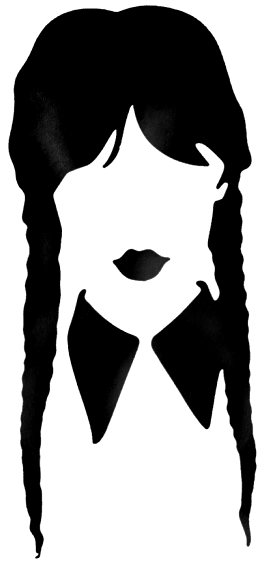
\includegraphics[height=1.35em]{figures/icons/mira-silhouette.png}}{}}}\enspace{\scshape\color{black}Scene}\enspace\textperiodcentered\enspace{\bfseries #1}\pdblockheadingend{\itshape #2}}%
    \end{tcolorbox}\par\addvspace{8pt plus 2pt}%
  }%
  \long\def\xrefbox#1{\par\pd@settle\addvspace{4pt}\noindent\pd@marginhead{See also}{\small #1}\par\addvspace{4pt}}%
  % A generic "Thesis" margin label does not identify which claim matters.
  % Keep the prose; use an authored keyidea head only when it adds meaning.
  \long\def\pdthesis#1{\par\pd@settle\addvspace{6pt plus 1pt}\noindent#1\par\addvspace{6pt plus 1pt}}%
  \long\def\pullquote#1{\pdthesis{#1}}%
}
\makeatother

% Shared visual language for the Book's figures -- version 2.
% Twin: book/figures/pd-figure-language.tex (byte-identical; edit both).
% The standard behind it, the migration from v1 and the QA loop live in
% skills/tikz-diagram-craft/ (SKILL.md, references/figure-standard.md).
%
% This file defines voices, hues, weights and marks -- not layouts.  Every
% figure still chooses a grammar from its reader question.
%
% ===========================================================================
% 1.  THE TYPE LADDER.  Three voices, one size, each tied to a role.
%       pd title   bold      panel titles, row and actor heads, column heads
%       pd label   upright   node text, state names, axis titles, tick words,
%                            relation words on an edge, badge numerals
%       pd note    italic    the one annotation a figure is allowed
%     `pd tag` is the label voice knocked out of the page, for a word that
%     must sit near a rule.  `pd kind` (small caps) is a one- or two-word kind
%     tag, never a title.  Every piece of figure text is mixed case; \texttt
%     only for identifiers that are literally code; math mode for symbols.
%
% 2.  THE COLOUR SYSTEM.  Hue is meaning, and the meanings cross chapters.
%     The figure's own subject is drawn in the CHAPTER hue (`pd focus ...`),
%     resolved from \pdcurrentchaptercolor, which the Book sets per chapter;
%     a fragment declares its standalone fallback with \pdfigurehue{...}.
%     Anything else the figure names takes its concept hue:
%       pd truth       pdcobalt   kernel, truth, the thing being specified
%       pd legible     pdteal     legibility, digest, inspection
%       pd ready       pdhealth   ready, coordinated, admitted, passing
%       pd protocol    pdindigo   protocol, federation, the wire
%       pd identity    pdviolet   identity, continuity, a card, an ID
%       pd reputation  pdrust     reputation, trust earned over time
%       pd value       pdgold     economy, value, settlement, payment
%       pd breach      pderror    breach, refusal, revocation, correction
%       pd warn        pdamber    warning; rules and stripes only, never text
%     Each concept X yields X, X rule, X arrow, X state, X fill, X datum and
%     X label.  Two to four hues a figure; colour is always doubled by shape,
%     dash, weight or a word (breach and warn are dashed as well as coloured).
%
% 3.  THE WEIGHT LADDER.  Exactly three weights, .5 / .9 / 1.6 pt
%     (1 : 1.8 : 3.2).  .5: hairline, guide, tick, artifact edge, fill edge,
%     mark outline, badge.  .9: rule, arrow, state edge, concept arrow.
%     1.6: spine, focus rule, focus and concept state edges, concept rule.
%     A reader sees which line is the subject.  Tips scale with the stroke.
%
% 4.  THE SURFACE LADDER.  pd state (page ground, ink edge) < pd artifact
%     (page ground, grey edge, subordinate) < pd focus state and the concept
%     states (24 % tint, edged in the same hue).  Text is always ink.  A
%     terminal state has a double boundary; an automaton's states are circles
%     (`pd automaton state/focus/terminal`); a ledger's pools are buckets
%     joined by pipes (`pd bucket`, `pd pipe`); a trust boundary is a dashed
%     rectangle (`pd trust boundary`).
%
% 5.  THE GROUND.  Body pages print on white, so every knockout and every
%     neutral surface is `pdpage` (white), never cream: a cream backing on a
%     white page reads as a sticker, which is what v1's figures were covered
%     in.  Neutral regions (Gantt bands, wells) are a warm grey tint.
%
% 6.  EDITIONS.  The Book sets \pdedition (maritime | swiss | technical) and
%     figures/pd-figure-language-<edition>.tex restyles the same names, so one
%     drawing renders in each edition's character.  A fragment that names a
%     raw colour (hhteal, pdcobalt!40, blue) bypasses this; name a role.
% ===========================================================================
% Libraries every v2 mark needs (diamonds, braces, markings), and
% pgfplots for computed plots. This file is \input in every preamble (the
% Book's and each standalone chapter's), so a plot works in all of them.
\usetikzlibrary{arrows.meta,matrix,patterns.meta,positioning,calc,fit,
  backgrounds,shapes.geometric,shapes.multipart,shapes.misc,decorations.pathreplacing,
  decorations.markings,quotes,intersections}
\RequirePackage{pgfplots}
\pgfplotsset{compat=1.18}
\usepgfplotslibrary{fillbetween,groupplots}

\colorlet{pdpage}{white}

% --- the chapter hue, resolved late --------------------------------------
% \pdfigurehue{pdindigo} on the line before a tikzpicture names the hue the
% figure is drawn in when it is compiled outside the Book (a standalone
% chapter, or the skill's renderer).  Inside the Book the preamble has already
% defined \pdcurrentchaptercolor and the chapter opener sets it, so there the
% opener wins and \providecommand does nothing.  Local to the figure's group.
\newcommand{\pdfigfraghue}{pdcobalt}
\newcommand{\pdfigurehue}[1]{%
  \renewcommand{\pdfigfraghue}{#1}%
  \providecommand{\pdcurrentchaptercolor}{#1}}
\newcommand{\pdsetfocushue}{%
  \ifdefined\pdcurrentchaptercolor
    \colorlet{pdfocus}{\pdcurrentchaptercolor}%
  \else
    \colorlet{pdfocus}{\pdfigfraghue}%
  \fi}
\colorlet{pdfocus}{pdcobalt}

% ===========================================================================
% THE TYPOGRAPHIC LAW
% ===========================================================================
% Companion to the line-weight law in figures/pd-palette.tex (1px texture,
% 1.5px linework, 2px enclosure). Same shape of rule: name the roles, fix the
% values, one place.
%
% ONE SIZE. Every named text role in a figure is \pdfiglabelsize
% (= \footnotesize). Roles separate by WEIGHT, SLOPE, FAMILY and INK -- never
% by size. A fragment never writes a size command of its own; if a distinction
% needs making, it takes the role that makes it.
%
% Where the size comes from. Measured, not chosen:
%   \tiny  \scriptsize  \footnotesize  \small  \normalsize
%   5.23    6.97          8.72           9.55    10.46  pt   Book (10.5pt
%                                                            Pagella, 4.5in
%                                                            column, 7x10in)
%   5.98    7.97          8.97           9.96    10.91  pt   standalone chapter
%                                                            (11pt Latin Modern)
% \scriptsize renders at 6.97pt in the Book -- under figcheck's 7pt T1 floor
% before a single width promotion, so it is illegal by measurement, not taste.
% \footnotesize holds 8.72pt and still clears the floor at the 0.85 \resizebox
% limit craft-rules sets (7.41pt). It is also what the corpus already voted
% for: 78 of the 91 local font= declarations this law replaces were already
% \footnotesize, \footnotesize\bfseries or \footnotesize\itshape.
%
% \pdfigbasesize (= \small) is the tikzpicture's ambient size only, so an
% unstyled node is never SMALLER than a styled one; every named role steps
% down exactly one notch from it and none steps down twice.
%
% ONE FACE, AND IT IS THE DOCUMENT'S. \pdfiglabelfamily is empty by default,
% which means figure type inherits whatever face the document is setting --
% Palatino in the Book, Computer Modern in a standalone chapter. Figures
% agreeing with EACH OTHER is not the goal; figures agreeing with the
% paragraph beside them is. A fragment therefore never names a family. Not
% \sffamily (which resolves to Latin Modern Sans against a Computer Modern
% page and reads as a foreign object on it), not \rmfamily, not
% \fontfamily{...}. P18 in tikz_precheck.py is an error for exactly that.
% An edition MAY substitute a face -- the Swiss and technical editions set
% \pdfiglabelfamily to \pdgrotesk, because grotesk display is their declared
% character -- and it does so in ONE command in ONE file, so the substitution
% is a decision on the record rather than an accident in a fragment. The
% only family a fragment may ask for is the identifier one, and it asks for
% it by role (pd mono label / \pdfiglabelmono), never by \ttfamily.
%
% What the roles are, and what each one is for:
%   pd panel title        bold        the name of a panel
%   pd row label          bold        an actor/row name east of its lane
%   pd reverse row label  bold, cream a row name sitting on a dark band
%   pd axis label         regular     an axis title or a tick numeral
%   pd direct label       regular     a value or name riding its own mark
%   pd reverse label      regular, cream  a direct label on a dark band
%   pd mono label         mono        an identifier, path, or literal
%   pd verdict            bold        a terminal outcome stamp (CLEAR, REJECT)
%   pd note               italic      one aside per figure
%   pd legend             regular     a pgfplots legend entry
%   pd state / terminal / actor / artifact / decision   node text
%   pd axis               the whole pgfplots typographic block, one key
%   \pdfigsub             a gloss line under a heading INSIDE a node
%   \pdfigmath            math carrying a sub/superscript, inside a label
%
% A fragment that needs a compound style of its own composes it from a role
% above (`gate/.style={pd decision,minimum width=2cm}`), or, where no role
% fits, from the \pdfiglabel* handles here. It never writes a raw size
% command: P16 in skills/harbor-chartwork/scripts/tikz_precheck.py is an
% error for exactly that, and P10/P11 have been errors for \tiny and
% \scriptsize since before this law.
%
% What does NOT transfer from the screen rules these roles otherwise follow.
% The dataviz method those rules come from assumes an interactive chart: a
% tooltip carries any value a label could not fit, a filter row rescopes the
% view, hover lifts the hovered mark. A printed page has none of that, and the
% absence is not a defect to design around. The INTENT of the tooltip rule --
% "every value is reachable without gating" -- does transfer, and on this page
% it is discharged somewhere else: the value is in the caption, in the margin
% apparatus, or in the chapter's own worked example. So a label that will not
% fit inside its mark moves outside the mark or is dropped to the caption; it
% is never shrunk to fit, because there is no size below \footnotesize to shrink
% to, and never clipped. Do not add a hover affordance, a legend toggle, or a
% filter to a figure in this book.
%
% IDENTIFIERS GET ONE SPELLING. A key, a cell id, a file name or any other
% literal a reader could type is set in `pd mono label` (or \pdfiglabelmono
% inside a compound style), spelled exactly as the code spells it: sk_A, not
% skA and not sk with a subscript A; card0, not card-nought and not a Unicode
% subscript zero. A figure that shows the same identifier two ways has told
% the reader they are two things. The subscripted form belongs to MATHEMATICS
% ($\kappa_7$, an index into a sequence) and the literal form to CODE -- one
% figure may use both, for different objects, but never both for the same
% one. (A precheck for two spellings of one identifier inside a fragment is
% being added on another branch; this is the convention it will enforce.)
%
% SHAPE IS A CHANNEL, AND IT HAS TO SURVIVE THE PRINT SIZE. pd datum, pd
% focus datum and pd caution datum carry three different forms, because the
% house palette is three low-chroma print inks and every distinction it makes
% has to be doubled by something that is not colour. That only counts if the
% form is still legible at 2.1-2.7 pt: an edition that flattens all three to
% one form has removed the second channel and left the figure separating its
% classes by hue alone, which fails in greyscale and for a colour-blind
% reader. Any edition override that restyles a datum must keep three
% distinguishable forms, and must be checked on a render at 1.0x, not
% reasoned about from the point sizes.
%
% One screen rule that does NOT bind here, and why. "Text never wears the data
% colour" exists because a light categorical hue is illegible as text on a
% light surface. The house figure hues are print inks, not screen hues --
% hhink #1B1712, hhteal #00564C, hhamber #6B4500 -- and all three clear text
% contrast on cream, so a label MAY wear its series' ink to bind itself to a
% curve, which is direct labelling and saves a legend. The rule that survives
% is the reason behind it: text wears one of those three inks at full
% strength, or hhink!80!hhgray for recessive furniture, and nothing else. A
% tint of an ink (text=hhgray, text=hhteal!60) is not a role; it is a fade.
% ===========================================================================

\providecommand{\pdfiglabelfamily}{}            % an edition may set \pdgrotesk
\providecommand{\pdfiglabelsize}{\footnotesize} % every named text role
\providecommand{\pdfigbasesize}{\small}         % the picture's ambient size
\providecommand{\pdfiglabel}{\pdfiglabelfamily\pdfiglabelsize}
\providecommand{\pdfiglabelbold}{\pdfiglabel\bfseries}
\providecommand{\pdfiglabelitalic}{\pdfiglabel\itshape}
\providecommand{\pdfiglabelmono}{\pdfiglabelsize\ttfamily}
% The one role that is not a node style, because it lives INSIDE a node's text:
% the second line under a heading that glosses it ("reviewer role / obligation +
% capability + authority"). Every fragment that needed it reached for \tiny or
% \scriptsize, which is how seven \tiny and twelve \scriptsize survived P10/P11
% as hard errors in the corpus. It steps down by SLOPE and WEIGHT, not size, so
% it stays legible and stays legal, and it touches neither family nor ink --
% which is what lets it sit on a reversed node without vanishing.
\providecommand{\pdfigsub}{\mdseries\itshape}
% The one place the law's own size is not the right size.
%
% Measured, both preambles, on a subscripted label inside `pd direct label`:
%
%              base glyph   subscript   subscript as % of base
%   chapter      8.97pt       5.98pt            66.7%
%   Book         8.72pt       6.36pt            72.9%
%   promoted    10.91/10.46   7.97/7.64
%
% An earlier version of this comment said those subscripts are "under figcheck's
% 7pt T1 floor". They are not, and the correction is worth more than the claim
% was. T1 has TWO bands: running text is held to 7.0pt, and a span of three
% glyphs or fewer -- a sub/superscript, a tick numeral -- is held to 5.9pt
% (T1_SHORT_SPAN_PT). That second band is not a loophole. A subscript is set at
% roughly 70% of its base by every typesetter that has ever existed; holding one
% to the running-text floor would mean either no subscripts in figures at all,
% or a figure whose base type is 10pt against 8.72pt body text.
%
% So \pdfigmath is NOT a T1 remedy, and using it as one is how a rule gets
% applied where it does not belong. It exists because 5.98pt clears the
% short-span band by 0.08pt, and 0.08pt is not a margin: a font substitution, an
% edition that nudges \pdfigbasesize, or a chapter that loads a different math
% font puts that subscript under the band with nobody having decided anything.
% Promotion puts it at 7.97/7.64pt -- over even the running-text floor -- while
% the base glyph stays close enough to its neighbours that the label still reads
% as one label.
%
% Use it ONLY for a math group that carries a sub- or superscript. Plain math
% takes the label's own size like any other text, and P22 in tikz_precheck.py is
% an error if it does not.
\providecommand{\pdfigmath}{\normalsize}

% ---------------------------------------------------------------------------
% THE GUIDE DASH, IN ABSOLUTE POINTS, IN ONE PLACE.
%
% `pd guide` used to read `line width=.45pt,densely dotted`. `densely dotted`
% expands to `dash pattern=on \pgflinewidth off 1pt`, and \pgflinewidth is read
% when the KEY is processed, not when the path is stroked. So the Swiss
% edition's `pd guide/.append style={draw=hhink!40,line width=.5pt}` widened the
% stroke and left the dash at the .45pt already baked into it. The canonical
% Book therefore shipped a 0.448pt dot on a 0.498pt stroke.
%
% MEASURED IN THE SHIPPED ARTIFACT, not in a probe: 50 guide strokes sampled
% pixel by pixel in the committed coordination-papers-mega-volume.pdf, at 150
% dpi / 1.0x.
%
%   on 0.448pt = 0.93 device px -- UNDER ONE PIXEL; off 0.996pt = 2.08 px
%   the dash DECLARES 69% of each line's length as gap
%   only 34% of each line's pixels actually reach paper
%   35.4% of three-period windows contain NO pixel that reaches paper at all
%
% That last number is the defect. The gap (2.08 px) is narrower than the
% antialias spread of a 0.93 px stroke, so as the pattern's phase drifts along a
% line the gaps fill in: over a third of every guide's length there is no gap
% left and it is a continuous grey stroke, while the rest of the same line still
% reads as dots. The ink arrives. The DOTTEDNESS does not. A reader sees one
% line that is dotted here and solid there, and no author chose that.
%
% Twenty-five of the corpus's thirty-six guide draws use dottedness to mean
% "this line is not a drawn edge", so twenty-five of them were making a
% distinction the page does not carry.
%
% After, same measurement, same probe geometry, Book preamble:
%   on 1.2pt = 2.50 px, off 2.0pt = 4.17 px, stroke .7pt = 1.45 px
%   0.0% of three-period windows are without paper -- every gap survives,
%     at every phase
%   50% of pixels reach paper against 62.5% declared, the shortfall now being
%     the stroke's antialias skirt rather than the whole signal
%
% ON THE INK, because the obvious reading of this change is wrong. The BASE pair
% was never the problem: hhgray!62 against the hairline's hhgray!78 is 0.411
% against 0.517 of nominal ink, well apart. The problem is that the Book renders
% the SWISS edition (\pdedition defaults to swiss; the committed Book PDF is
% full of hhink!40 guides), where the pair was hhink!40 against hhink!45 -- 4.6%
% of the grey scale. Deleting the Swiss override, which is the right fix for the
% geometry, makes the base ink govern the Book too -- and hhgray!62 is 0.411
% against the Book hairline's 0.410. The same grey, to a thousandth. So the base
% ink has to move, or the dash would go back to carrying the whole distinction
% by itself, which is how this started.
%
% hhink!70 measured against the hairline, mean ink on the page at 150 dpi:
%   chapter  guide 0.0502  hairline 0.0790   guide is 64% of the hairline
%   Book     guide 0.0545  hairline 0.0671   guide is 81% of the hairline
% Per DOT it is 0.638 against 0.410 -- unmistakably a different mark. In MEAN it
% is still lighter than the hairline -- so it still recedes. Two channels, both
% working, instead of one that does not.
%
% The replacement is stated absolutely and measures phase-STABLE: every dot
% renders at the same weight wherever it falls on the grid (peak column ink
% 0.808, invariant across twelve sub-pixel offsets). It is a macro rather than
% three numbers because an edition that restates one of them and not the others
% is how this defect happened. The geometry is a LEGIBILITY FLOOR, not an
% edition's character: an edition may move the guide's ink, and states the
% geometry through these two macros so it cannot half-restate it.
%
% Any dash in this corpus is stated in absolute points. The `dotted` family
% (`dotted`, `densely dotted`, `loosely dotted`) derives its on-length from the
% line width and is therefore banned -- P23 in tikz_precheck.py. `dashed` and
% its relatives are absolute (on 3pt off 3pt) and are fine.
\providecommand{\pdguidewidth}{.7pt}
% Three lengths, not one macro holding the whole key: pgfkeys splits a key list
% on `,` and `=` before expanding anything (so a macro carrying `dash
% pattern=...` is read as one key NAME), and TikZ's dash-pattern scanner reads
% the literal words `on`/`off` without expanding a macro that hides them. A
% dimension after each word does expand, which is the seam that works.
\providecommand{\pdguideon}{1.2pt}
\providecommand{\pdguideoff}{2.0pt}

\tikzset{
  % --- picture level: one size, one default tip, the chapter hue -----------
  % A figure label is a name, not prose: it never hyphenates.
  pd figure/.style={font=\pdfiglabelfamily\pdfigbasesize,text=pdink,line cap=round,line join=round,
    >={Stealth[length=2.6pt 3.2,width=2.0pt 2.4]},/utils/exec=\pdsetfocushue,
    every node/.append style={execute at begin node={%
      \hyphenpenalty=10000\exhyphenpenalty=10000\relax}}},
%
  % --- 1. the voices ---------------------------------------------------------
  pd title/.style={font=\pdfiglabelbold,text=pdink,align=center},
  pd label/.style={font=\pdfiglabel,text=pdink,align=center},
  pd note/.style={font=\pdfiglabelitalic,text=pdinkmuted,align=left},
  pd kind/.style={font=\pdfiglabel\scshape,text=pdinkmuted,align=center},
  pd tag/.style={pd label,fill=pdpage,inner sep=1.7pt},
%
  % --- 4. surfaces -----------------------------------------------------------
  pd state/.style={pd label,draw=pdink,line width=.9pt,fill=pdpage,
    rounded corners=1pt,inner xsep=6pt,inner ysep=4.5pt,minimum height=7.4mm},
  % a terminal state carries a double boundary, as every automaton text draws it
  pd terminal/.style={pd state,double=pdpage,double distance=1.1pt,line width=.5pt},
  pd artifact/.style={pd label,draw=pdinkmuted!60,line width=.5pt,fill=pdpage,
    rounded corners=1pt,inner xsep=5pt,inner ysep=3.5pt,minimum height=6.2mm},
  pd panel/.style={draw=pdinkmuted!55,line width=.5pt,
    dash pattern=on 2.4pt off 2pt,rounded corners=2.5pt,inner sep=7pt,align=center},
  pd hatch/.style={pattern={Lines[angle=45,distance=4pt,line width=.3pt]},
    pattern color=pdinkmuted!70},
  pd neutral fill/.style={fill=pdinkmuted!12,draw=pdinkmuted!55,line width=.5pt},
%
  % --- 3. strokes ------------------------------------------------------------
  pd hairline/.style={draw=pdinkmuted!45,line width=.5pt},
  % Absolute dash, from the typographic law's three macros above: a guide is a
  % definite dotted construction line, darker per dot than the hairline and
  % lighter in mean ink. A lattice is the quiet continuous grid a figure stands on.
  pd guide/.style={draw=pdink!70,line width=\pdguidewidth,dash pattern=on \pdguideon off \pdguideoff},
  pd lattice/.style={draw=pdinkmuted!40,line width=.4pt},
  pd tick/.style={draw=pdinkmuted!75,line width=.5pt},
  pd rule/.style={draw=pdink,line width=.9pt},
  pd spine/.style={draw=pdink,line width=1.6pt},
  pd thin arrow/.style={draw=pdinkmuted!75,line width=.5pt,->},
  pd arrow/.style={pd rule,->},
  pd spine arrow/.style={pd spine,->},
%
  % --- the chapter hue, as the figure's focus --------------------------------
  pd focus rule/.style={draw=pdfocus,line width=1.6pt},
  pd focus arrow/.style={pd focus rule,->},
  pd focus state/.style={pd state,draw=pdfocus,line width=1.6pt,fill=pdfocus!24},
  % The single solid chapter-colour surface in a figure: use only for the
  % culmination or object the reader should name after five seconds. Editions
  % may render ordinary focus with a pale field while keeping this one solid.
  pd climax state/.style={pd focus state},
  % a member of the subject's set when the set, not one node, is the subject:
  % edged in the chapter hue, never filled, so the one solid node stays unique
  pd focus outline/.style={pd state,draw=pdfocus,line width=1.2pt,fill=pdpage},
  pd focus fill/.style={fill=pdfocus!24,draw=pdfocus,line width=.5pt},
  pd focus datum/.style={circle,fill=pdfocus,draw=pdpage,line width=.5pt,inner sep=2.6pt},
  pd focus label/.style={pd label,text=pdfocus!85!pdink},
%
  % --- marks -----------------------------------------------------------------
  pd datum/.style={circle,fill=pdink,draw=pdpage,line width=.5pt,inner sep=2.3pt},
  pd badge/.style={pd label,circle,draw=pdink,line width=.5pt,fill=pdpage,
    inner sep=.5pt,minimum size=5.0mm},
  pd focus badge/.style={pd badge,draw=pdfocus,line width=.9pt,fill=pdfocus!24},
  % --- conventions shared by every chapter (Critical Analysis, 2026-09-08) ---
  % Automata: states are circles, terminal (accepting) states double circles;
  % edge words are short action names; guards go in an aligned legend table.
  pd automaton state/.style={pd label,circle,draw=pdink,line width=.9pt,fill=pdpage,
    minimum size=11mm,inner sep=1pt},
  pd automaton focus/.style={pd automaton state,draw=pdfocus,line width=1.6pt,fill=pdfocus!24},
  pd automaton terminal/.style={pd automaton state,double=pdpage,double distance=1.1pt,
    line width=.5pt},
  pd initial/.style={draw=pdink,line width=.9pt,->},
  % Ledgers: asset pools are rectangular buckets (open at the top) joined by
  % directed pipes; the conserved sum is set as an equation under the rails.
  pd bucket/.style={pd label,draw=none,minimum width=2.2cm,minimum height=1.3cm,
    append after command={\pgfextra{\draw[draw=pdink,line width=.9pt]
      (\tikzlastnode.north west) -- (\tikzlastnode.south west)
      -- (\tikzlastnode.south east) -- (\tikzlastnode.north east);}}},
  pd pipe/.style={draw=pdink,line width=.9pt,double=pdpage,double distance=2.2pt,
    -{Stealth[length=3.4pt 2,width=5.2pt]}},
  pd focus pipe/.style={pd pipe,draw=pdfocus},
  % Trust boundaries: a dashed rectangle is the Dolev-Yao interface; a vector
  % that escapes it is drawn in pd breach and named.
  pd trust boundary/.style={draw=pdink,line width=.9pt,dash pattern=on 4pt off 2.4pt,
    rounded corners=0pt,inner sep=8pt},
  % a stroke that ends at a badge is shortened, so no rule touches the numeral
  pd to badge/.style={shorten >=2pt},
  pd from badge/.style={shorten <=2pt},
}

% ===========================================================================
% 7.  PLOTS.  A plot is computed by a committed script, never sketched.  `pd
%     axis` is the one axis grammar: two spines (left, bottom), ticks out, no
%     box, no grid unless asked (`pd grid`), tick words in the label voice,
%     numbers with a thin-space thousands separator, room outside the plot for
%     direct labels (clip=false).  Series are named at their ends, not in a
%     legend: `pd series` (ink), `pd focus series` (chapter hue), and
%     `pd X series` for a concept; breach and warn series are dashed.  A
%     region between curves is `pd focus fill`/`X fill` with fillbetween.
%     Width: `width=` is the plot box (scale only axis); leave about 1.6 cm
%     of the 11.4 cm column for the y tick words and title.
% ===========================================================================
\pgfplotsset{
  pd axis/.style={
    scale only axis,width=8.8cm,height=4.6cm,
    axis lines*=left,axis line style={draw=pdink,line width=.5pt,-},
    tick align=outside,major tick length=3pt,minor tick length=0pt,
    tick style={draw=pdink,line width=.5pt},
    tick label style={pd label,text=pdinkmuted},
    label style={pd label},title style={pd title},
    every axis title/.append style={yshift=-2pt},
    enlargelimits=false,clip=false,
    grid=none,
    legend style={draw=none,fill=none,font=\pdfiglabel},
    /pgf/number format/1000 sep={\,},
    every axis plot/.append style={line width=.9pt,line join=round,mark size=1.7pt},
  },
  pd grid/.style={ymajorgrids,major grid style={draw=pdinkmuted!30,line width=.4pt}},
  pd series/.style={draw=pdink,mark=*,mark options={fill=pdink,draw=pdpage,line width=.5pt,solid}},
  pd focus series/.style={draw=pdfocus,line width=1.6pt,mark=*,
    mark options={fill=pdfocus,draw=pdpage,line width=.5pt,solid}},
  pd muted series/.style={draw=pdinkmuted!70,line width=.9pt,mark=none},
}
\newcommand{\pdplotconcept}[2]{%
  \pgfplotsset{#1 series/.style={draw=#2,mark=*,
    mark options={fill=#2,draw=pdpage,line width=.5pt,solid}}}}
\pdplotconcept{pd truth}{pdcobalt}
\pdplotconcept{pd legible}{pdteal}
\pdplotconcept{pd ready}{pdhealth}
\pdplotconcept{pd protocol}{pdindigo}
\pdplotconcept{pd identity}{pdviolet}
\pdplotconcept{pd reputation}{pdrust}
\pdplotconcept{pd value}{pdgold}
\pgfplotsset{
  pd breach series/.style={draw=pderror,dash pattern=on 3.2pt off 2.2pt,mark=diamond*,
    mark options={fill=pderror,draw=pdpage,line width=.5pt,solid}},
  pd warn series/.style={draw=pdamber,dash pattern=on 3.2pt off 2.2pt,mark=none},
}

% ===========================================================================
% Supplied visual-guide primitives: native Book type, deliberate strokes,
% readable Stealth heads, open markers, and a quiet quantitative grid.
% These are opt-in: old diagrams need spacing review before thicker arrows.
\tikzset{
  pd guide step/.style={pd artifact,draw=pdink,fill=pdpage,line width=1pt,
    align=center,minimum height=40pt,inner xsep=5pt,inner ysep=6pt},
  pd guide arrow/.style={draw=pdcobalt,line width=1.15pt,
    -{Stealth[length=7pt,width=4.4pt]},shorten <=2pt,shorten >=2pt},
}
\newcommand{\pdflowstep}[4]{%
  \node[pd guide step,text width=#4] (#1) at #2 {#3};}
\newcommand{\pdflowlink}[2]{%
  \draw[pd guide arrow] (#1.east)--(#2.west);}
\pgfplotsset{
  pd evidence axis/.style={pd axis,
    axis line style={draw=pdink,line width=1pt,-},
    tick style={draw=pdink,line width=.8pt},
    grid=major,major grid style={draw=pdinkmuted!20,line width=.35pt},
    axis background/.style={fill=pdpage}},
  pd evidence measured/.style={draw=pdcobalt,line width=1.35pt,mark=*,
    mark size=2.6pt,mark options={fill=pdpage,draw=pdcobalt,line width=1.1pt}},
  pd evidence comparison/.style={draw=pdink,line width=1.1pt,
    dash pattern=on 4pt off 2.5pt,mark=square*,mark size=2.2pt,
    mark options={fill=pdink,draw=pdink,solid}},
}
% Analytic curves, not sampled observations. Integer samples preserve the
% meaning of reviewer count; callers set axes and name their assumptions.
\newcommand{\pdindependentmisses}[2]{%
  \addplot[pd evidence measured,domain=1:#2,samples=#2] {100*(1-#1)^x};}
\newcommand{\pdreviewcost}[1]{%
  \addplot[pd evidence measured,domain=1:#1,samples=#1] {x};}
% 8.  UML.  The Book's engineering diagrams use UML 2.5 notation, so a reader
%     who knows UML reads them without a key.  Four kinds:
%     STATE MACHINE  `pd uml state` (rounded), `pd uml focus state`, a
%       composite drawn with `pd uml composite` around its substates plus a
%       compartment of internal transitions; `pd uml initial` (filled dot),
%       `pd uml final` (bullseye), `pd uml choice` (diamond); transitions are
%       `pd uml transition` (open arrowhead) labelled  event [guard] / effect.
%     SEQUENCE  `pd uml head` (lifeline head), `pd uml lifeline` (dashed),
%       `pd uml activation` (thin bar), messages `pd uml sync` (filled head),
%       `pd uml async` (open head), `pd uml reply` (dashed, open head),
%       `pd uml fragment` + `pd uml fragment tag` for alt / opt / loop.
%     COMPONENT  `pd uml component` with \pdumlicon{node} (the component
%       glyph) and a <<component>> keyword; `pd uml port`; provided interface
%       \pdumlprovided{from}{to}{name} (lollipop), required \pdumlrequired (socket).
%     ERD (crow's foot)  `pd er entity` (rectangle split: name, then rows;
%       mark keys PK / FK in the row text), relationship lines `pd er rel`
%       with tips `er one`, `er many`, `er zero or one`, `er one or many`,
%       `er zero or many` at either end.
% ===========================================================================
\pgfdeclarearrow{
  name = pd crow,
  parameters = {\the\pgfarrowlength,\the\pgfarrowwidth},
  setup code = {%
    \pgfarrowssettipend{0pt}%
    \pgfarrowssetlineend{0pt}%
    \pgfarrowssetbackend{-\pgfarrowlength}%
    \pgfarrowsupperhullpoint{0pt}{.5\pgfarrowwidth}%
    \pgfarrowsupperhullpoint{-\pgfarrowlength}{0pt}%
    \pgfarrowssavethe\pgfarrowlength
    \pgfarrowssavethe\pgfarrowwidth},
  drawing code = {%
    \pgfsetdash{}{0pt}%
    \pgfpathmoveto{\pgfqpoint{-\pgfarrowlength}{0pt}}%
    \pgfpathlineto{\pgfqpoint{0pt}{.5\pgfarrowwidth}}%
    \pgfpathmoveto{\pgfqpoint{-\pgfarrowlength}{0pt}}%
    \pgfpathlineto{\pgfqpoint{0pt}{-.5\pgfarrowwidth}}%
    \pgfusepathqstroke},
  defaults = {length=2.4mm, width=3.0mm}
}
\tikzset{
  % state machine
  pd uml state/.style={pd state,rounded corners=4.5pt},
  pd uml focus state/.style={pd focus state,rounded corners=4.5pt},
  pd uml terminal/.style={pd terminal,rounded corners=4.5pt},
  pd uml composite/.style={draw=pdink,line width=.9pt,rounded corners=7pt,fill=none,inner sep=0pt},
  pd uml initial/.style={circle,fill=pdink,draw=none,minimum size=2.4mm,inner sep=0pt},
  pd uml final/.style={circle,draw=pdink,line width=.9pt,fill=pdpage,minimum size=3.6mm,inner sep=0pt,
    path picture={\fill[pdink] (path picture bounding box.center) circle (1.1mm);}},
  pd uml choice/.style={diamond,draw=pdink,line width=.9pt,fill=pdpage,minimum size=4.2mm,inner sep=0pt},
  pd uml transition/.style={pd rule,-{Straight Barb[length=2.2pt 2.2,width=4.4pt 2.2]}},
  pd uml focus transition/.style={pd focus rule,-{Straight Barb[length=2.2pt 2.2,width=4.4pt 2.2]}},
  pd uml breach transition/.style={pd rule,draw=pderror,dash pattern=on 3.2pt off 2.2pt,
    -{Straight Barb[length=2.2pt 2.2,width=4.4pt 2.2]}},
  % sequence
  pd uml head/.style={pd state,rounded corners=0pt,minimum height=6.8mm},
  pd uml lifeline/.style={draw=pdinkmuted!75,line width=.5pt,dash pattern=on 3pt off 2pt},
  pd uml activation/.style={draw=pdink,line width=.5pt,fill=pdpage,minimum width=2.2mm,inner sep=0pt},
  pd uml sync/.style={pd rule,-{Triangle[length=3.2pt 1.6,width=3.2pt 1.6]}},
  pd uml async/.style={pd rule,-{Straight Barb[length=2.4pt 2,width=4.4pt 2]}},
  pd uml reply/.style={pd rule,dash pattern=on 3pt off 2pt,-{Straight Barb[length=2.4pt 2,width=4.4pt 2]}},
  pd uml fragment/.style={draw=pdink,line width=.5pt,fill=none,inner sep=6pt},
  pd uml fragment tag/.style={pd label,font=\footnotesize\bfseries,draw=pdink,line width=.5pt,fill=pdpage,
    inner xsep=3pt,inner ysep=2pt,chamfered rectangle,chamfered rectangle corners=south east,
    chamfered rectangle xsep=2pt},
  % component
  pd uml component/.style={pd state,rounded corners=0pt,align=center,inner xsep=8pt,inner ysep=6pt,minimum height=11mm},
  pd uml port/.style={rectangle,draw=pdink,line width=.5pt,fill=pdpage,minimum size=2mm,inner sep=0pt},
  % ERD
  pd er entity/.style={pd label,rectangle split,rectangle split parts=2,rectangle split part align={center,left},
    draw=pdink,line width=.9pt,fill=pdpage,inner xsep=5pt,inner ysep=3pt,align=left,
    rectangle split part fill={pdinkmuted!12,pdpage}},
  pd er rel/.style={pd rule},
  er one/.tip={Bar[width=3.0mm,sep=1.2pt]Bar[width=3.0mm]},
  er many/.tip={Bar[width=3.0mm,sep=1.4pt]pd crow},
  er zero or one/.tip={Circle[open,length=1.8mm,width=1.8mm,sep=1.2pt,fill=pdpage]Bar[width=3.0mm]},
  er one or many/.tip={Bar[width=3.0mm,sep=1.4pt]pd crow},
  er zero or many/.tip={Circle[open,length=1.8mm,width=1.8mm,sep=1.2pt,fill=pdpage]pd crow},
}
% the component glyph, drawn in the top-right corner of a component node
\newcommand{\pdumlicon}[1]{%
  \begin{scope}[shift={($(#1.north east)+(-4.2mm,-2.6mm)$)},x=1mm,y=1mm]
    \draw[pdink,line width=.5pt,fill=pdpage] (0,-1.1) rectangle (2.6,1.1);
    \draw[pdink,line width=.5pt,fill=pdpage] (-.6,.25) rectangle (.6,.65);
    \draw[pdink,line width=.5pt,fill=pdpage] (-.6,-.65) rectangle (.6,-.25);
  \end{scope}}
% a provided interface (lollipop) from a node side to a point, with its name
\newcommand{\pdumlprovided}[3]{%
  \draw[pd rule] (#1) -- (#2);
  \draw[pd rule,fill=pdpage] (#2) circle (1.3mm);
  \node[pd label,anchor=south] at ($(#2)+(0,1.6mm)$) {#3};}
% a required interface (socket): a half-circle open toward the provider
\newcommand{\pdumlrequired}[4]{% from, to, name, facing angle of the socket's opening
  \draw[pd rule] (#1) -- (#2);
  \draw[pd rule] ($(#2)+(#4+90:1.9mm)$) arc[start angle=#4+90,end angle=#4+270,radius=1.9mm];
  \node[pd label,anchor=north] at ($(#2)+(0,-2.4mm)$) {#3};}

% --- 2. the concept map, as styles, so a drawing never chooses a hue --------
% An edition file may \renewcommand\pdconcept before the map below expands.
\newcommand{\pdconcept}[2]{%
  \tikzset{%
    #1/.style={draw=#2,text=pdink},
    #1 rule/.style={draw=#2,line width=1.6pt},
    #1 arrow/.style={draw=#2,line width=.9pt,->},
    #1 state/.style={pd state,draw=#2,line width=1.6pt,fill=#2!24},
    #1 fill/.style={fill=#2!24,draw=#2,line width=.5pt},
    #1 datum/.style={circle,fill=#2,draw=pdpage,line width=.5pt,inner sep=2.6pt},
    #1 label/.style={pd label,text=#2!85!pdink},
  }}

% --- 6. the edition layer, loaded before the concept map expands ----------
\ifdefined\pdedition\IfFileExists{figures/pd-figure-language-\pdedition.tex}{\input{figures/pd-figure-language-\pdedition}}{}\fi

\pdconcept{pd truth}{pdcobalt}
\pdconcept{pd legible}{pdteal}
\pdconcept{pd ready}{pdhealth}
\pdconcept{pd protocol}{pdindigo}
\pdconcept{pd identity}{pdviolet}
\pdconcept{pd reputation}{pdrust}
\pdconcept{pd value}{pdgold}
\pdconcept{pd breach}{pderror}
\pdconcept{pd warn}{pdamber}
% Breach and warning read as refusals, so they are dashed as well as
% coloured, and a breach mark is a diamond where every other mark is a circle.
% Amber is never text (3.71:1 on white); a warn label is set in ink.
\tikzset{
  pd breach rule/.append style={dash pattern=on 3.2pt off 2.2pt},
  pd breach arrow/.append style={dash pattern=on 3.2pt off 2.2pt},
  pd warn rule/.append style={dash pattern=on 3.2pt off 2.2pt},
  pd warn arrow/.append style={dash pattern=on 3.2pt off 2.2pt},
  pd breach datum/.append style={diamond},
  pd warn label/.style={pd label},
}

% ===========================================================================
% v1 NAMES.  Kept so every existing fragment still compiles; they resolve to
% the v2 roles, so an untouched figure inherits the ladder.  New work uses the
% v2 names (skills/tikz-diagram-craft/references/migration-v1-to-v2.md).
% ===========================================================================
\tikzset{
  pd row label/.style={pd title,anchor=east},
  pd panel title/.style={pd title,align=left},
  pd axis label/.style={pd label},
  % Direct labels sit beside their mark; they do not erase a line or box
  % underneath themselves. A label that needs a paper knockout is misplaced
  % and must be moved, not given an invisible patch.
  pd direct label/.style={pd tag,fill=none,align=left},
  pd actor/.style={pd state},
  pd boundary/.style={pd panel},
  pd caution rule/.style={pd breach rule},
  pd caution arrow/.style={pd breach arrow},
  pd caution fill/.style={pd breach fill},
  pd caution datum/.style={pd breach datum},
}

% ===========================================================================
% Roles named on main by the typographic law (#10191), expressed on the v2
% roles so an edition's .append style on the parent reaches them. `pd danger`
% is main's name for what v2 calls `pd breach` (red, dashed, diamond marks);
% both names resolve to one family. Main's hairline-boxed fact badge is
% `pd fact badge`: v2's `pd badge` is the numbered guard/step marker.
% ===========================================================================
\tikzset{
  pd danger rule/.style={pd breach rule},
  pd danger arrow/.style={pd breach arrow},
  pd danger fill/.style={pd breach fill,text=pdink},
  pd danger datum/.style={pd breach datum},
  pd ink fill/.style={fill=pdink,draw=pdink,line width=.4pt,text=pdpage},
  pd decision/.style={pd state,diamond,aspect=1.55,font=\pdfiglabelbold,
    minimum height=0pt,inner xsep=3pt,inner ysep=3pt},
  pd mono label/.style={pd direct label,font=\pdfiglabelmono,inner xsep=2.5pt,inner ysep=2.5pt},
  pd verdict/.style={pd direct label,font=\pdfiglabelbold},
  pd reverse label/.style={pd direct label,text=pdpage,fill=none},
  pd reverse row label/.style={pd row label,text=pdpage},
  pd legend/.style={font=\pdfiglabel,text=pdink,draw=none,fill=none},
  pd kind tag/.style={pd kind,align=right},
  pd fact badge/.style={pd hairline,font=\pdfiglabel,text=pdink,align=center,
    inner sep=2.4pt,fill=none},
}

% Small reusable marks.  They deliberately avoid prose-bearing boxes.
\newcommand{\pdfigaxis}[4]{%
  \draw[pd rule,->] (#1,#2) -- (#3,#2);
  \node[pd label,anchor=west] at (#3,#2) {#4};
}
\newcommand{\pdfigvaxis}[4]{%
  \draw[pd rule,->] (#1,#2) -- (#1,#3);
  \node[pd label,anchor=south] at (#1,#3) {#4};
}

% Native-size, object-based evidence figures; shared by Book and chapters.
% Shared approved Swiss evidence drawing primitives. Keep both chapter roots identical.
\ifdefined\pdSwissEvidenceLoaded\else
\def\pdSwissEvidenceLoaded{1}
% Real ink-box gate; no declared coordinate envelope can substitute for this.
\newsavebox{\sgEvidenceBox}
\newcommand{\SGMeasuredFigure}[2]{%
  \sbox{\sgEvidenceBox}{#2}%
  \typeout{SG-GEOMETRY: #1,width=\the\wd\sgEvidenceBox,height=\the\dimexpr\ht\sgEvidenceBox+\dp\sgEvidenceBox\relax}%
  \ifdim\wd\sgEvidenceBox>325.215pt
    \PackageError{swiss-evidence}{Figure #1 exceeds the Book column}{Recompose at native text size; do not scale.}%
  \fi
  \usebox{\sgEvidenceBox}}
% Parent redraws after rejection of lab specimens 01,04,06.
% All coordinates are physical TeX points; no resizebox or transformed fonts.
\usetikzlibrary{arrows.meta,calc}
% Aliased onto the house palette (figures/pd-palette.tex), not \definecolor'd
% as independent HTML values: an edition that restyles pdcobalt/pdteal/...
% now restyles every SG figure with it. The six values were already
% bit-identical matches for pdcobalt/pdteal/pdviolet/pdamber/pderror/pdink;
% the alias turns that into a guarantee instead of a coincidence.
\colorlet{sgBlue}{pdcobalt}
\colorlet{sgTeal}{pdteal}
\colorlet{sgViolet}{pdviolet}
\colorlet{sgAmber}{pdamber}
\colorlet{sgRed}{pderror}
\colorlet{sgInk}{pdink}
\definecolor{sgGrid}{HTML}{D8C7A6}
% The one house size, inheriting the document's own face (the typographic
% law in pd-figure-language.tex): no \sffamily leak, no local \fontsize.
\newcommand{\SGType}{\pdfiglabel}
\tikzset{sg/base/.style={x=1pt,y=1pt,line cap=butt,line join=miter,
  every node/.style={font=\SGType,inner sep=0pt,text=sgInk}},
  sg/arrow/.style={-{Stealth[length=4.5pt,width=3.6pt]},draw=sgInk,line width=.85pt},
  sg/grid/.style={draw=sgGrid,line width=.3pt},
  sg/hash/.style={draw=sgBlue,fill=sgBlue!7,line width=1pt,minimum width=53pt,
    minimum height=27pt,inner sep=4pt,align=center},
  sg/sibling/.style={draw=sgAmber,fill=sgAmber!10,line width=1pt,minimum width=51pt,
    minimum height=27pt,inner sep=4pt,align=center},
  sg/check/.style={draw=sgInk,fill=white,line width=1pt,minimum width=92pt,
    minimum height=30pt,inner sep=5pt,align=center}}

% A folded record, not an undifferentiated rounded node. Width/height are pt.
\newcommand{\SGDocument}[6]{%
  \begin{scope}[shift={#2}]
    \path[draw=sgInk,fill=#5,line width=.85pt]
      (0,0)--({#3-7},0)--(#3,7)--(#3,#4)--(0,#4)--cycle;
    \draw[sgInk,line width=.65pt] ({#3-7},0)--({#3-7},7)--(#3,7);
    \node[minimum width=#3pt,minimum height=#4pt,text width=\dimexpr#3pt-12pt\relax,
      align=center] (#1) at ({#3/2},{#4/2}) {#6};
  \end{scope}}

\newcommand{\SGSurvival}{%
\begin{tikzpicture}[sg/base]
  % Three complete probability decades, percentages rather than tiny exponents.
  \foreach \x in {0,1,...,6}{\draw[sg/grid] ({35+30*\x},20)--({35+30*\x},140);}
  \foreach \y/\lab in {20/{0.1\%},60/{1\%},100/{10\%},140/{100\%}}{%
    \draw[sg/grid] (35,\y)--(215,\y);
    \draw[sgInk,line width=.65pt] (32,\y)--(35,\y);
    \node[anchor=east] at (28,\y) {\lab};}
  \draw[sgInk,line width=.85pt] (35,140)--(35,20)--(215,20);
  \foreach \x in {0,2,4,6}{%
    \draw[sgInk,line width=.65pt] ({35+30*\x},20)--({35+30*\x},17);
    \node[anchor=north] at ({35+30*\x},12) {$\x$};}
  \node[rotate=90] at (-9,80) {jobs still running (log scale)};
  \node[anchor=north] at (125,-5) {duration / mean duration};
  \draw[sgBlue,line width=1.5pt,domain=0:6,samples=100]
    plot ({35+30*\x},{140-120*ln(1+\x/2)/ln(10)});
  \draw[sgViolet,line width=1.2pt,dash pattern=on 4pt off 2.5pt,domain=0:6,samples=100]
    plot ({35+30*\x},{140-40*\x/ln(10)});
  % Endpoint leaders have allocated space; text does not lie on a curve.
  \draw[sgBlue,line width=.8pt] (215,67.75)--(224,67.75);
  \node[anchor=west,text=sgBlue,font=\SGType\bfseries] at (230,73) {Lomax};
  \node[anchor=west,text=sgBlue] at (230,60) {1.56\%};
  \draw[sgViolet,line width=.8pt,dashed] (215,35.77)--(224,35.77);
  \node[anchor=west,text=sgViolet,font=\SGType\bfseries] at (230,40) {exponential};
  \node[anchor=west,text=sgViolet] at (230,27) {0.248\%};
\end{tikzpicture}}

\newcommand{\SGTiming}{%
\begin{tikzpicture}[sg/base,y=-1pt]
  % This bracket spans COMMIT TO SYNC. It is not a range of hypothetical syncs.
  \path[draw=sgAmber!35,fill=sgAmber!9,line width=.5pt] (39,19) rectangle (253,49);
  \draw[sgAmber,line width=1pt] (39,18)--(39,9)--(253,9)--(253,18);
  \node[anchor=south,text=sgAmber,font=\SGType\bfseries] at (146,5) {?};
  \draw[sgInk,line width=.9pt] (39,27)--(39,45) (253,27)--(253,45);
  \draw[{Stealth[length=4.5pt,width=3.6pt]}-{Stealth[length=4.5pt,width=3.6pt]},
    sgAmber,line width=1.3pt] (40,36)--(252,36);
  \node[anchor=north,font=\SGType\bfseries] at (39,52) {commit};
  \node[anchor=north,font=\SGType\bfseries] at (253,52) {WAL sync};
  \node[anchor=west] at (0,86) {heartbeats received};
  \foreach \x/\label in {57/{s_1},117/{s_2},194/{s_3},278/{s_4}}{%
    \draw[sgViolet!70,dashed,line width=.55pt] (\x,104)--(\x,145);
    \node[anchor=south,text=sgViolet] at (\x,101) {$\label$};}
  \path[draw=sgAmber!35,fill=sgAmber!9,line width=.5pt] (158,108) rectangle (243,142);
  \draw[sg/grid] (0,139)--(306,139);
  \draw[sgTeal,line width=1.4pt]
    (0,132)--(25,132)--(25,116)--(33,116)--(33,132)
    --(85,132)--(85,116)--(93,116)--(93,132)
    --(145,132)--(145,116)--(153,116)--(153,132)--(306,132);
  \draw[sgRed,line width=1pt] (243,106)--(243,145);
  \node[anchor=north,text=sgRed] at (243,149) {deadline};
  \draw[sg/arrow] (0,174)--(306,174);
  \node[anchor=north east] at (306,179) {time};
\end{tikzpicture}}

\newcommand{\SGInclusion}{%
\begin{tikzpicture}[sg/base,y=-1pt]
  % Two independent inputs: a supplied proof and an issuer-authenticated root.
  \node[anchor=north west,font=\SGType\bfseries,text width=158pt,align=left] at (0,0)
    {Recompute from the receipt};
  \node[anchor=north west,font=\SGType\bfseries,text width=118pt,align=left] at (193,0)
    {Authenticate\\the checkpoint};
  \draw[sg/grid,step=15pt] (0,29) grid (175,194);
  \SGDocument{receipt}{(4,35)}{49}{34}{sgViolet!9}{receipt $P$}
  \node[sg/hash] (leaf) at (29,103) {$a=H_L(P)$};
  \node[sg/sibling] (sibone) at (108,103) {sibling $b$};
  \node[sg/hash] (inner) at (68,146) {$u=H_N(a,b)$};
  \node[sg/sibling] (sibtwo) at (146,146) {subtree $c$};
  \node[sg/hash,fill=sgBlue,text=white,minimum width=100pt] (computed) at (107,190)
    {$R'=H_N(u,c)$};
  \draw[sg/arrow,draw=sgViolet] (receipt.south)--(leaf.north);
  \draw[sg/arrow,draw=sgBlue] (leaf.south)--(inner.north west);
  \draw[sg/arrow,draw=sgAmber] (sibone.south)--(inner.north east);
  \draw[sg/arrow,draw=sgBlue] (inner.south)--(computed.north west);
  \draw[sg/arrow,draw=sgAmber] (sibtwo.south)--(computed.north east);
  \SGDocument{checkpoint}{(211,37)}{85}{48}{sgTeal!8}{signed root $R^*$\\size $n=4$\\signature $\sigma$}
  % The trusted key is an external input, not something the prover supplies.
  \draw[sgInk,line width=1pt] (218,113) circle (3.5pt);
  \draw[sgInk,line width=1pt] (221.5,113)--(233,113) (230,113)--(230,117) (233,113)--(233,117);
  \node[anchor=west] at (239,113) {trusted $pk_I$};
  \node[sg/check,minimum width=84pt] (verify) at (260,158) {verify $\sigma$\\result $A$};
  \draw[sg/arrow,draw=sgTeal] (checkpoint.east)--(311,61)--(311,158)--(verify.east);
  \draw[sg/arrow] (247,123)--(247,138)--(verify.north);
  \node[sg/check,minimum width=112pt,minimum height=34pt] (compare) at (164,245)
    {$A\ \land\ (R'=R^*)$};
  \draw[sg/arrow,draw=sgBlue] (computed.south)--(107,220)--(compare.north west);
  \draw[sg/arrow,draw=sgTeal] (verify.south)--(260,214)--(compare.north east);
  \node[anchor=east,text=sgTeal] at (250,204) {$R^*,A$};
  \node[draw=sgTeal,fill=sgTeal,text=white,minimum width=90pt,
    minimum height=27pt,font=\SGType\bfseries] (accept) at (76,299) {accept inclusion};
  \node[draw=sgRed,fill=white,text=sgRed,line width=1.2pt,minimum width=90pt,
    minimum height=27pt,font=\SGType\bfseries] (reject) at (256,299) {reject proof};
  \draw[sg/arrow,draw=sgTeal] (compare.south west)--(108,279)--(76,279)--(accept.north);
  \draw[sg/arrow,draw=sgRed] (compare.south east)--(220,279)--(256,279)--(reject.north);
  \node[anchor=south,text=sgTeal] at (82,275) {true};
  \node[anchor=south,text=sgRed] at (248,275) {false};
\end{tikzpicture}}

% Reusable geometry; load after swiss-redraws.tex. Real points, no scaling.
\newcommand{\SGDatabase}[4]{%
  \begin{scope}[shift={#2}]
    \path[draw=#3,fill=#3!7,line width=.9pt]
      (0,4)--(0,32) arc[start angle=180,end angle=360,x radius=24pt,y radius=5pt]
      --(48,4) arc[start angle=0,end angle=-180,x radius=24pt,y radius=5pt];
    \draw[draw=#3,fill=#3!7,line width=.9pt] (24,4) ellipse[x radius=24pt,y radius=5pt];
    \node[minimum width=48pt,minimum height=37pt,align=center] (#1) at (24,18) {#4};
  \end{scope}}

% Reader question: How do overlapping requests become ordered records?
% Evidence: schematic two-client history, not a runtime observation.
% Each request precedes commit 1; each reply follows its own committed record.
\newcommand{\SGWriterSequence}{%
\begin{tikzpicture}[sg/base,y=-1pt]
  % Recomposed at native size: a 22-character mono request label no longer
  % fits a 118pt lane gap at \pdfiglabelmono, so the HTTP verb is shortened
  % to the identifier it names and the resource it names ("auth.ts") moves
  % to the lane header, where it reads once instead of twice.
  \foreach \x/\lanelabel in {35/{{\pdfigmath$\alpha_{\text{auth}}$} (claude)},153/{Kernel (single writer)},275/{{\pdfigmath$\alpha_{\text{bill}}$} (codex)}}{
    \node[anchor=south,font=\pdfiglabelbold,align=center] at (\x,0) {\lanelabel};
    \draw[sg/grid] (\x,9)--(\x,237);}
  % Both invocations precede the first commit: overlapping client requests.
  \draw[sg/arrow,draw=sgViolet] (35,29)--(153,29);
  \node[anchor=south,text=sgViolet,font=\pdfiglabelmono] at (94,24) {POST /claims};
  \draw[sg/arrow,draw=sgAmber] (275,57)--(153,57);
  \node[anchor=south,text=sgAmber,font=\pdfiglabelmono] at (214,52) {POST /claims};
  % commit 1 succeeds: drawn in the kernel's own hue. commit 2 is the
  % kernel's WAL record of a REFUSAL, not a second grant -- it is drawn in
  % the breach hue so the outcome is doubled by colour, not stated in prose
  % alone (the typographic law's "colour is always doubled" rule). The
  % "lock held" highlight band is gone: at native size it ran directly
  % behind this text, which figcheck reads as a drawn line through the
  % words, and the sequencing arrows already carry the serialization claim.
  \SGDocument{commitA}{(93,71)}{120}{46}{sgBlue!8}{{\pdfiglabelbold commit 1 \textperiodcentered{} WAL 4102}\\[2pt]{\pdfigsub {\pdfigmath$\alpha_{\text{auth}}$} \textperiodcentered{} epoch 104}}
  \draw[sg/arrow,draw=sgViolet,dash pattern=on 3pt off 2pt] (153,130)--(35,130);
  \node[anchor=south,text=sgViolet,font=\pdfiglabel] at (94,128) {201 Created};
  \SGDocument{commitB}{(93,152)}{120}{46}{sgRed!8}{{\pdfiglabelbold commit 2 \textperiodcentered{} WAL 4103}\\[2pt]{\pdfigsub {\pdfigmath$\alpha_{\text{bill}}$} refused}}
  \draw[sg/arrow,draw=sgAmber,dash pattern=on 3pt off 2pt] (153,213)--(275,213);
  \node[anchor=south,text=sgAmber,font=\pdfiglabel] at (214,211) {409 Conflict};
  \draw[sg/arrow] (3,20)--(3,232);
  \node[anchor=west,font=\pdfiglabel] at (9,236) {time};
\end{tikzpicture}}

% Reader question: What is checked before the service admits requests?
% Source: SQLite WAL documentation, sections 2--2.2, cited in the chapter.
% Checkpointing copies committed pages; it does not apply uncommitted work.
% The dashed group denotes separate mechanisms, not a proved composition.
\newcommand{\SGRecoveryAdmission}{%
\begin{tikzpicture}[sg/base,y=-1pt]
  % Recomposed at native size: a 25-character mono command (sqlite3_wal_
  % checkpoint_v2) no longer fits a 103pt-wide column once the label grows
  % from 5.0pt to \pdfiglabelmono, so the three mechanisms read top to
  % bottom, full measure, instead of left to right in three narrow lanes.
  \draw[sgInk!55,dash pattern=on 3pt off 2pt,line width=.7pt]
    (0,0) rectangle (300,318);

  % 1. Checkpoint WAL
  \node[anchor=north west,align=left,text width=228pt] at (10,8)
    {{\pdfiglabelbold 1. Checkpoint WAL}\\[2pt]
     {\pdfiglabelmono\color{sgBlue} sqlite3\_wal\_checkpoint\_v2}\\[2pt]
     {\pdfigsub Copies committed WAL pages into the main database; uncommitted frames are not applied.}};
  \SGDocument{walback}{(247,4)}{34}{26}{sgViolet!7}{}
  \SGDocument{walfront}{(253,9)}{34}{26}{sgViolet!7}{WAL}
  \draw[sg/arrow] (18,101)--(18,118);

  % 2. Check Pages
  \node[anchor=north west,align=left,text width=228pt] at (10,122)
    {{\pdfiglabelbold 2. Check Pages}\\[2pt]
     {\pdfiglabelmono\color{sgTeal} PRAGMA integrity\_check}\\[2pt]
     {\pdfigsub Verifies B-tree pointers and freelist allocation across every page.}};
  \SGDatabase{db}{(251,118)}{sgBlue}{SQLite}
  \draw[sg/arrow] (18,215)--(18,232);

  % 3. Verify Links
  \node[anchor=north west,align=left,text width=228pt] at (10,236)
    {{\pdfiglabelbold 3. Verify Links}\\[2pt]
     {\pdfiglabelmono\color{sgAmber} Merkle chain verify}\\[2pt]
     {\pdfigsub Validates cryptographic audit-log continuity link by link.}};
  \foreach \x in {249,267,285}{
    \draw[sgAmber,line width=1pt,rounded corners=2pt] (\x,240) rectangle ({\x+14},256);}
  \draw[sgAmber,line width=1pt] (259,248)--(267,248) (281,248)--(289,248);

  % Decision Gate
  \node[sg/check,minimum width=165pt,minimum height=28pt,font=\pdfiglabelbold] (admit) at (150,350)
    {all critical checks pass?};
  \draw[sg/arrow] (150,318)--(admit.north);

  \node[draw=sgTeal,fill=sgTeal,text=white,minimum width=125pt,minimum height=32pt,
    align=center] (serve) at (65,420) {{\pdfiglabelbold admit requests}\\[1.5pt]{\pdfigsub HTTP 200 Ready (:9876)}};
  \node[draw=sgRed,fill=white,text=sgRed,line width=1pt,minimum width=125pt,
    minimum height=32pt,align=center] (refuse) at (235,420) {{\pdfiglabelbold refuse service}\\[1.5pt]{\pdfigsub HTTP 503 Unavailable}};

  \draw[sg/arrow,draw=sgTeal] (admit.south west)--(90,384)--(65,384)--(serve.north);
  \draw[sg/arrow,draw=sgRed] (admit.south east)--(210,384)--(235,384)--(refuse.north);
  % Each tag sits clear of its own diagonal leg, on the side the diagonal
  % does NOT occupy -- PASS left of its bend, FAIL right of its bend --
  % rather than centred on the bend where the stroke crosses the glyphs.
  \node[anchor=south east,text=sgTeal,font=\pdfiglabelbold] at (63,382) {PASS};
  \node[anchor=south west,text=sgRed,font=\pdfiglabelbold] at (237,382) {FAIL (HALT)};
\end{tikzpicture}}

% Named bands and their audiences; the dashed floor is NOT a fifth layer.
\newcommand{\SGStackLayers}{%
\begin{tikzpicture}[sg/base,y=-1pt]
  \foreach \y/\level/\name/\audience/\evidence/\hue in {
    0/3/Economy/{Between operators}/{settlement and reputation}/sgAmber,
    51/2/Legibility/{For the operator}/{summaries linked to evidence}/sgTeal,
    102/1/Coordination/{Between agents}/{permissions and commitments}/sgViolet,
    153/0/Substrate/{On one machine}/{ordered writes and records}/sgBlue}{
    \path[draw=\hue,fill=\hue!8,line width=1pt] (17,\y) rectangle (142,{\y+38});
    \node[anchor=west,font=\SGType\bfseries,text=\hue] at (26,{\y+13}) {L\level};
    \node[anchor=west,font=\SGType\bfseries] at (26,{\y+27}) {\name};
    \node[anchor=north west,font=\SGType\bfseries] at (158,{\y+2}) {\audience};
    \node[anchor=north west,text width=149pt,align=left] at (158,{\y+17}) {\evidence};}
  \foreach \y in {153,102,51}{\draw[sg/arrow] (79,\y)--(79,{\y-13});}
  \draw[sgBlue,line width=2.4pt] (7,154)--(7,190);
  \draw[sgInk!60,dashed,line width=.7pt] (17,204) rectangle (307,243);
  \node[anchor=west,font=\SGType\bfseries] at (26,216) {Machine floor};
  \node[anchor=west] at (26,231) {file lock, clock, socket, supervisor};
  \draw[sg/arrow] (79,204)--(79,192);
\end{tikzpicture}}

% Compact counterpart for future chapter-by-chapter marginal navigation.
% A named current-layer argument changes emphasis, never the layer order.
\newcommand{\SGMarginLadder}[1]{%
\begin{tikzpicture}[sg/base,y=-1pt]
  \foreach \y/\n/\name/\hue in {0/3/Economy/sgAmber,37/2/Legibility/sgTeal,74/1/Coordination/sgViolet,111/0/Substrate/sgBlue}{
    \draw[\hue,line width=.7pt] (0,\y)--(91,\y);
    \node[anchor=north west,text=\hue,font=\SGType\bfseries] at (4,{\y+3}) {L\n};
    \node[anchor=north west] at (4,{\y+16}) {\name};
    \ifnum\n=#1\relax\draw[\hue,line width=2pt] (0,{\y+3})--(0,{\y+29});\fi}
\end{tikzpicture}}

\fi



% The proof-obligation markers (\Closed/\Partial/\Open) come from
% figures/pd-pedagogy.tex (\input above), so this chapter has them available
% for the implementation-status appendix it does not yet carry -- without a
% second definition of its own. This skeleton pass uses none of them.


% ─── Listings Setup ─────────────────────────────────────────────────────
\lstdefinestyle{proverif}{
  language=C,
  backgroundcolor=\color{codebg},
  frame=single,
  rulecolor=\color{codeframe},
  basicstyle=\ttfamily\small,
  keywordstyle=\color{darkblue}\bfseries,
  commentstyle=\color{darkgreen}\itshape,
  stringstyle=\color{accent},
  numbers=left,
  numberstyle=\tiny\color{gray},
  numbersep=8pt,
  breaklines=true,
  showstringspaces=false,
  tabsize=2,
  xleftmargin=15pt,
  xrightmargin=5pt,
  framexleftmargin=15pt,
  captionpos=b
}
\lstset{style=proverif}

% ─── Theorem Environments ──────────────────────────────────────────────
\theoremstyle{definition}
\newtheorem{definition}{Definition}[section]
\newtheorem{theorem}{Theorem}[section]
\newtheorem{lemma}{Lemma}[section]
\newtheorem{property}{Property}[section]

% ─── Header/Footer ───────────────────────────────────────────────────────
\pagestyle{fancy}
\fancyhf{}
\fancyhead[L]{\small\textit{The Sealed Harbor}}
\fancyhead[R]{\small\thepage}
\fancyfoot[C]{\footnotesize\color{hhgray} Port Daddy Coordination Papers \textperiodcentered\ Chapter~\pdchapternumber\ of \pdchaptercount}
\renewcommand{\headrulewidth}{0.4pt}
\renewcommand{\footrulewidth}{0pt}

% ─── Title ──────────────────────────────────────────────────────────────────
\title{
  \vspace{-1cm}
  {\Large\textsc{Port Daddy Coordination Papers \textperiodcentered\ Chapter~\pdchapternumber\ of \pdchaptercount}}\\[
0.5cm]
  \rule{\textwidth}{0.5pt}\\[0.3cm]
  {\LARGE\textbf{The Sealed Harbor:}}\\[0.2cm]
  {\Large Mutually Confidential Computation with\\Explicit, Gated, Bounded Releases}\\[0.3cm]
  \rule{\textwidth}{0.5pt}
}
\author{
  \textbf{Erich Owens}\\[0.2cm]
  Curiositech LLC\\[0.2cm]
  \texttt{engineering@portdaddy.dev}
}
\date{\pdeditiondate\\Version 1.0 (textbook edition)}
% ─── Document ────────────────────────────────────────────────────────────
% Hyperlink and cross-reference discipline (must stay last in the preamble).
% Shared hyperlink and cross-reference discipline for the Book and its chapters.
% Load this LAST in every preamble: cleveref must follow hyperref and amsthm.
% hyperref itself is loaded earlier with [backref=page] (a load-time option).
% Twin copy under book/figures/ (byte-identical; checked by
% scripts/generate-mega-whitepaper.test.mjs).
%
% What a reader gets: live links on chapter titles, section numbers, theorems,
% figures, tables, equations, page numbers, and citations; PDF bookmarks three
% levels deep; and, at the end of every bibliography entry, the pages that cite it.
% Links are quiet: a warm dark ink one step lighter than body text, so the
% four part hues keep their meaning and an inline chapter title never competes
% with the part it sits in. Chrome pages (the front-matter map, part openers)
% recolor their own links locally.
\hypersetup{
  colorlinks=true,
  linkcolor=pdinkmuted,
  citecolor=pdinkmuted,
  urlcolor=pdinkmuted,
  filecolor=pdinkmuted,
  anchorcolor=pdink,
  bookmarksnumbered=true,
  bookmarksdepth=3,
  bookmarksopen=true,
  bookmarksopenlevel=1,
  breaklinks=true,
  linktoc=all,
  pdfauthor={Erich Owens},
  pdftitle={\pdchaptertitle},
  pdfsubject={\pdeditiontitle: \pdeditionsubtitle},
}

% Title-based chapter references. \pdchaplink{prefix}{text} is a live link to
% the chapter inside the Book (the Book's preamble defines it before loading this
% file); in a standalone chapter it is plain text. Prose uses \pdchapref, which
% sets the title in italics; the locator map uses \pdchaplink directly.
\providecommand{\pdchaplink}[2]{#2}
\DeclareRobustCommand{\pdchapref}[2]{\pdchaplink{#1}{\emph{#2}}}

% \ifpdbook -- true in the assembled Book, false otherwise.
%
% WHY THIS EXISTED. A drawing that two chapters both \input prints twice in the
% Book, under two figure numbers. The fix is for the chapter that develops the
% idea to keep the figure and the other to point at it -- but the standalone
% edition of a chapter had nowhere to point, and rewriting the prose outright
% removed five figures from harbor-economy-whitepaper.pdf and left it telling a
% conference reader that a ceremony is "drawn in The Federated Harbor", a
% document that reader did not have.
%
% WHERE IT STANDS NOW. The per-chapter PDFs are retired: the Book is the one
% document, so \ifpdbook is true in every build that renders, and the \else
% branches are source with no output. They are still here, and still read by
% check_duplicate_figures.py (which must not count an \else \input as a Book
% input) -- but nothing prints them, and nothing new should be put in one.
% Whether to delete them is an open question; see the retirement PR.
%
% The divergence was per-build. A CONDITIONAL and not a two-argument macro:
% the generator inlines each \input, so a figure branch is a whole table or
% tikzpicture, and as a macro argument that is scanned as one token list --
% which is how \pdinbook produced "runaway argument" on the first attempt.
% \ifpdbook skips the untaken branch at the TeX level instead.
%
% Declared unconditionally and defaulting FALSE, which is the standalone
% answer. The Book's preamble sets \pdbooktrue immediately after loading
% this file. A guard here would have to mention \ifpdbook or \newif inside a
% branch TeX may skip, and a conditional token in skipped text is counted as
% a nested \if -- which is how two attempts at a guard both produced
% "Incomplete \ifdefined". Ordering is cheaper than cleverness.
\newif\ifpdbook

% cleveref: "Theorem 3.1", "Figure 2.4", "Section 1.3", capitalised, never
% abbreviated, with the whole phrase clickable. Names are declared explicitly
% because the theorem environments are created before this file is loaded.
\usepackage[nameinlink,capitalise,noabbrev]{cleveref}
\crefname{pdchapter}{Chapter}{Chapters}
\crefname{part}{Part}{Parts}
\crefname{appendix}{Appendix}{Appendices}
\crefname{definition}{Definition}{Definitions}
\crefname{theorem}{Theorem}{Theorems}
\crefname{lemma}{Lemma}{Lemmas}
\crefname{proposition}{Proposition}{Propositions}
\crefname{corollary}{Corollary}{Corollaries}
\crefname{conjecture}{Conjecture}{Conjectures}
\crefname{property}{Property}{Properties}
\crefname{protocol}{Protocol}{Protocols}
\crefname{lsprotocol}{Protocol}{Protocols}
\crefname{stpprotocol}{Protocol}{Protocols}
\crefname{heprotocol}{Protocol}{Protocols}
\crefname{remark}{Remark}{Remarks}
\crefname{lstlisting}{Listing}{Listings}
\crefname{exercise}{Exercise}{Exercises}
\crefname{solution}{Solution}{Solutions}
\Crefname{pdchapter}{Chapter}{Chapters}
\Crefname{lstlisting}{Listing}{Listings}
\Crefname{exercise}{Exercise}{Exercises}
\Crefname{solution}{Solution}{Solutions}

% Back-references: "^ Cited on pages 12, 40, and 87." after every bibliography
% entry, each page number a live link back to the page that cited the work.
% Distinct pages only (#3/#4).
%
% The page numbers used to be wrapped in \color{hhgray} along with the words,
% which painted over the link colour hyperref had just given them: the links
% were there -- 29 annotations on a typical bibliography page -- and looked
% exactly like the grey prose around them, so nobody knew they could click.
% Restoring the quiet link colour would not have fixed it either; pdinkmuted
% against hhgray is 1.53:1, which is no signal at footnote size.
%
% So the numbers take pdcobalt (7.55:1 on the cream, and a hue a reader cannot
% mistake for grey), and the line opens with the return arrow this book already
% uses to send a solution back to its exercise. This is a deliberate exception
% to the quiet-link discipline above, and the reason is that back-matter
% navigation is the one place where the link IS the content: in prose the
% surrounding sentence tells you a phrase is a destination, and in a
% bibliography nothing does.
\renewcommand*{\backref}[1]{}
\renewcommand*{\backrefalt}[4]{%
  \ifcase #3\relax
  \or {\footnotesize{\color{hhgray}$\uparrow$~Cited on page}~{\hypersetup{linkcolor=pdcobalt}#4}{\color{hhgray}.}}%
  \else {\footnotesize{\color{hhgray}$\uparrow$~Cited on pages}~{\hypersetup{linkcolor=pdcobalt}#4}{\color{hhgray}.}}%
  \fi}
\renewcommand*{\backrefsep}{, }
\renewcommand*{\backreftwosep}{ and }
\renewcommand*{\backreflastsep}{, and }

\begin{document}
\pdopensolutions
\setlength{\emergencystretch}{2em}
\maketitle
\thispagestyle{empty}
\vspace{1cm}
% ---------------------------------------------------------------------------
% The Sealed Harbor: chapter body, part 1 (problem, design, noninterference,
% enforceability). Part 2 carries conservation,
% detection, the leakage budget, limitations, recitation, and exercises.
% ---------------------------------------------------------------------------
\section{Two owners, one answer}\label{sec:sealed-problem}
\noindent\emph{Express lane: what can a sealed room promise when an agent
computes on data that its owner will not hand over? It promises that every
release is explicit, passes through a gate, and has a counted limit, which is
less than a promise that nothing leaks. In the running example, 200 jobs that
each return 64 bits to Erin can carry at most 12,800 bits, before timing.}

\begin{pdboundary}
\setlength{\parskip}{4pt plus 1pt}
Nothing in this chapter's room has been built. What exists are four toy
checkers, small Python scripts that each search or compute over a small model:
the two-run search, the controllability check, the ledger check and the leak
detector's arithmetic (Table~\ref{tab:sealed-four-links}).

The confidential virtual machine, the two release gates, the privacy ledger,
the leak detector and the in-guest monitor that forms the inner fence are
specified here and not implemented. The sandbox that would hold the inner
fence has not been chosen.
\end{pdboundary}

\paragraph{The scene.}
Derek owns sensitive financial data $D$. Erin owns a valuable agent system $M$:
weights, prompts, skills, tools, orchestration. Both want the answer
$y=f_M(D)$. Neither will hand over the crown jewels they own. Derek must not receive $M$,
Erin must not receive $D$, and the cloud operator hosting the computation must
receive neither. Figure~\ref{fig:sealed-three-principals} draws the three
parties, their three sight-lines, and the one boundary that must keep all
three apart at once.
% Reader question: where may Derek's data and Erin's model meet in plaintext?
% Claim: only the attested workload admits both; all three principals remain
% outside its confidentiality boundary. Release is separately authorized.
% Evidence: sealed-harbor.tex, sec:sealed-problem and sec:sealed-design.
% Grammar: containment plus directed inputs; not a triangle enclosed by a room.
% Counter-read: an attested workload is not proof against every hardware channel.
\begin{figure}[H]
\centering
\pdfigurehue{pdcobalt}%
\begin{tikzpicture}[pd figure,x=1cm,y=1cm]
  \node[pd actor,minimum width=2.6cm] (D) at (1.4,4.4)
    {Derek\\owns data $D$};
  \node[pd actor,minimum width=2.6cm] (E) at (8.8,4.4)
    {Erin\\owns model $M$};
  \draw[pd trust boundary] (2.5,.4) rectangle (7.7,3.3);
  \node[pd title,anchor=north] at (5.1,3.12) {attested confidential workload};
  \node[pd focus state,minimum width=3.6cm] (W) at (5.1,2.1)
    {compute with $D$ and $M$};
  \node[pd label,anchor=north,text width=4.2cm] at (5.1,1.35)
    {plaintext meets only here};
  \draw[pd arrow] (D.south) -- (1.4,2.1) -- (W.west);
  \node[pd label] at (1.25,1.65) {encrypted $D$};
  \draw[pd arrow] (E.south) -- (8.8,2.1) -- (W.east);
  \node[pd label] at (8.95,1.65) {encrypted $M$};
  \node[pd actor,minimum width=3.3cm] (H) at (5.1,-.7)
    {cloud operator\\hosts the workload};
  \draw[pd guide] (H.north) -- (5.1,.4);
  \node[pd note,anchor=north,text width=9.8cm,align=center] at (5.1,-1.45)
    {Derek receives no model plaintext; Erin receives no data plaintext.\\
     The host is outside the confidentiality boundary.};
\end{tikzpicture}
\caption{The sealed room contains the computation, not its owners or host.
Derek supplies data and Erin supplies a model over encrypted input channels;
attestation binds their release to the intended workload. Authorized outputs
leave through separate release gates. The claim assumes the chapter's
confidential-computing boundary and does not eliminate excluded hardware
side channels.}
\label{fig:sealed-three-principals}
\end{figure}

The question is what the machine running the job can guarantee when the data
owner and the agent owner distrust each other. Call that machine, with its
controls, a sealed room: a closed computing environment that both owners'
secrets enter and from which only agreed answers leave. It must protect both
owners and still let the agreed answer out. A contract can list the releases
the owners permit; their legal relationship is a separate matter. A single
writer orders the accounting, but by itself it cannot confine the worker or
decide what an answer reveals. Section~\ref{sec:sealed-history} compares the
design with Ryoan and SCONE (Table~\ref{tab:sealed-ryoan}). First, look at the
output the owners actually want to permit.

\paragraph{Why blocking tainted outputs is insufficient.}
Consider a proposed ``silicon-enforced NDA'': tag Erin's agent the moment it
reads Derek's data, drop any tainted egress packet, and declare that the data
``mathematically cannot phone home.'' The first job of this chapter is to say
why that sentence is false, and the second is to prove the sentence that
replaces it.
\begin{pdexample}{What ``Nothing Leaks'' Costs, in Bits}
\setlength{\parskip}{4pt plus 1pt}
Compare the three candidate designs on the chapter's own toy release, the one
that Property~\ref{thm:sealed-noninterference} later checks exhaustively. The
whole comparison fits in your head. For this example Derek's secret is uniform on
$\{0,1,2,3\}$, so its entropy is $\log_2 4 = 2$ bits, and the contracted release is
\[
g(s)=s\bmod 2,
\]
which takes two values and therefore carries exactly $1$ bit. Written in
binary, $s$ has its parity in the low position, so the release is one of the
secret's two bits.

Now count. An honest gate
hands Erin $1$ of those $2$ bits: the bit Derek sold her, and no more.

A leaky gate that forwards $s$ itself hands over $2$ bits, the whole secret,
which is why the checker catches it four steps in.
Section~\ref{sec:sealed-noninterference} plants exactly this gate as a
deliberate bug.

A taint tracker of the kind pitched above, run \emph{soundly} on every token,
must mark the parity bit as tainted, because it was computed from the secret,
and drop it. Erin gets $0$ bits.

So a sound taint tracker gives Erin nothing, not even the bit she paid for. The
other horn of the dilemma, a tracker loosened to let the parity bit through,
has the opposite flaw. It
cannot tell whether the released bit is the parity of committed $s$, Derek's
actual record, or the parity of some other value $f(s)$ the worker computed
from that record in order to smuggle out a different bit.

Every workable design therefore releases something between nothing and
everything, and the rest of the chapter measures how much it may release.
\end{pdexample}

To keep track of whose secrets a value may carry, the room attaches an
\pdterm{owner label} to every value it holds. The label is the set of owners
whose permission is still needed before that value may leave.

\begin{pdclaim}{Design invariant}{Conservative Whole-Worker Labeling}
\setlength{\parskip}{4pt plus 1pt}
\label{hyp:sealed-taint}
Once the worker reads an owner's secret, everything the worker emits
afterwards keeps that owner's label until an authorized release removes it.
The design does not rely on any tool that tries to tell, token by token,
which parts of a model's output depend on the secret.

This is a cautious engineering choice. The literature on label creep and
dynamic monitoring \pdcite{denning77,rs10} explains why a tracker that is both
precise and permissive is hard to build. A restricted model or a trusted
release computation could justify a finer policy. The room assumes neither for
its untrusted worker.
\end{pdclaim}
\pdscope{The choice is a design rule for an untrusted worker; it says nothing
about how fine a sound analysis of model output could be.}

A secret can leave the room riding inside wording, punctuation, error
messages, output length or timing, and no regular expression, scanner or second model can certify that
arbitrary prose contains no secret. An ordinary remote model API also reads
the plaintext it is sent. Sending Derek's data to a third party's inference
endpoint hands the data to that third party, and no cryptography undoes it.

The architecture therefore controls the \emph{channel} through which output
leaves, and makes no attempt to vet each token. It turns the question a
security officer will ask, \emph{how do I know the wall has no other holes?},
into four claims that can be checked. The gate is the only hole in the wall,
the only way out (Section~\ref{sec:sealed-noninterference}). The gate can refuse the effects
that its mediation and observation model covers
(Section~\ref{sec:sealed-enforceability}). A conserved budget meters what
passes through it (Section~\ref{sec:sealed-conservation}). And a leak is
caught with a stated probability by a \pdterm{canary}, a decoy record planted
in the secret data that no legitimate output contains, with a model-based
estimate of how many outputs detection takes
(Section~\ref{sec:sealed-detection}). Section~\ref{sec:sealed-budget} combines
the four into one leakage account, and Section~\ref{sec:sealed-limitations}
states what none of this promises.

\section{One signed contract, two fences, two gates}\label{sec:sealed-design}

\paragraph{A diagnostic subtask for the checkout repair.}
Bob's failing checkout test may require a diagnosis using confidential
transaction records held by Derek and a diagnostic model held by Erin.
Bob's ownership of the repository grants authority over neither asset.
Alice therefore cannot delegate access she never received. Derek and Erin
need a separate agreement specifying what computation may use their secrets
and which result may reach the repair team. An authorized diagnostic answer
can inform a patch; it gives no permission to export the records or the model.

That agreement is the \pdterm{work order}: the contract both owners sign
before the job starts, fixing what the job may read, run and release. Before
listing its fields, try changing one term. Derek approves an in-room
diagnostic tool, but the worker asks to replace it with an external inference
endpoint. The tool list and permitted recipients change. A broker checking the
signed canonical work order must refuse the changed contract until both owners
approve it; accepting the old signature would ignore the very permission the
digest is meant to bind. A signature alone does not make the broker perform
that check.

\paragraph{The work order contract.}
Mutual confinement between owners who distrust each other starts from the
work order contract $C$, which both sign. In ordinary enterprise practice,
confidentiality rests on non-disclosure agreements. Lawyers draft
obligations, employees sign them, and violations are litigated after the
secret is out. A lawsuit can award a remedy; it cannot prevent the loss.
Weights copied to an external endpoint cannot be unseen, and a financial
dataset leaked over an unmetered socket cannot be unlearned.

The parties therefore need the technical boundary in place first. Before any
decryption key is released, both Derek (the data
owner) and Erin (the model and skill owner) sign the same work order $C$,
written in one canonical form:
{\small\[
\begin{aligned}
C=\bigl\langle\, & H(\text{data manifest}),\,H(\text{agent bundle}),\,H(\text{runtime}),\,H(\text{policy}),\\
& \text{function},\,\text{tools},\,\text{recipients},\,\text{output schemas},\,\text{budgets},\\
& \text{retention},\,\text{validators},\,\text{payment},\,\text{liability}\,\bigr\rangle.
\end{aligned}
\]}
Read the tuple in order. The thirteen fields play five roles. \emph{Pins} fix
by digest exactly which data, agent, runtime and policy are approved.
\emph{Permissions} say what may run, \emph{recipients} who may receive what,
\emph{bounds} how much the job may use and release, and \emph{remedies} what
happens after a breach. If $H$ is collision-resistant, any change to the
canonical contract changes the digest the signatures cover. A key broker that
follows the protocol refuses a modified contract until both owners sign again;
the digest by itself stops nothing.
The contract is a durable work unit in the sense of \pdchapref{swk}{The
Single-Writer Kernel}: a record that cannot change, a case file that outlives
every short-lived guest process that executes it.

Table~\ref{tab:sealed-work-order-elements} lists the thirteen elements of $C$,
the check each is meant to drive, and an illustrative value. A field states an
obligation; something else must enforce it. Two terms in the table need
defining first. A \pdterm{declassification} is an owner's authorized removal
of their label from a value, and it is the only way a value computed from a
secret may leave the room. \pdterm[differential privacy]{Differential privacy}
is a property of a randomized release in which adding or removing any one
record changes the probability of each set of outputs by at most a factor
$e^{\varepsilon}$, plus a small additive slack $\delta$. The human a record is
about is its \pdterm{data subject}. The number $\varepsilon$, read
\pdterm{epsilon}, is the release's privacy loss: smaller is more private.
The budgets row uses two more symbols. For a release channel whose content
the worker chooses, $b$ is the channel's width, the number of bits one
release on it may carry, and $q$ is the number of releases on it that the
work order allows over its whole term. In this chapter's examples each job
makes one release to Erin, so $q$ also counts jobs.

{\footnotesize
\setlength{\tabcolsep}{3pt}
\renewcommand{\arraystretch}{1.08}
\begin{xltabular}{\textwidth}{@{}
  >{\raggedright\arraybackslash}p{0.20\textwidth}
  >{\raggedright\arraybackslash}p{0.18\textwidth}
  >{\raggedright\arraybackslash}X
  >{\raggedright\arraybackslash\ttfamily\scriptsize}p{0.27\textwidth}@{}}
\caption{The thirteen elements of Work Order Contract $C$. Proposed contract fields and illustrative values. Measurements, permissions, and budgets require corresponding enforcement; payment and liability specify remedies rather than proving confidentiality.}\label{tab:sealed-work-order-elements}\\
\toprule
\textbf{Element} & \textbf{Role} & \textbf{Security Specification \& Guarantee} & \normalfont\textbf{Example Value} \\
\midrule
\endfirsthead
\multicolumn{4}{@{}l}{\small\itshape Table~\ref{tab:sealed-work-order-elements}: The thirteen elements of Work Order Contract $C$ (continued)}\\
\addlinespace[3pt]
\toprule
\textbf{Element} & \textbf{Role} & \textbf{Security Specification \& Guarantee} & \normalfont\textbf{Example Value} \\
\midrule
\endhead
\bottomrule
\multicolumn{4}{r}{\itshape\scriptsize Continues on next page $\,\blacktriangleright$} \\
\endfoot
\bottomrule
\endlastfoot
$H(\text{manifest})$ & Pins & Cryptographic digest over dataset chunks, schema layout, and provenance. Binds approved bytes; the loader must check them and reject other inputs. & sha256:7f83b165... \newline s3://derek/q3.parquet \\
\addlinespace[2pt]
$H(\text{agent})$ & Pins & Digest of model weights, tokenizer, prompt AST, and tools. Binds Erin's approved bundle; integrity also requires checked loading and protected execution. & sha256:c0ffee4b... \newline weights.safetensors \\
\addlinespace[2pt]
$H(\text{runtime})$ & Pins & Measured guest enclave launch digest (SEV-SNP / TDX MRTD) verifying kernel and monitor before execution. & mrtd:e4a8109d... \newline (Linux 6.8 + monitor) \\
\addlinespace[2pt]
$H(\text{policy})$ & Pins & Digest of declassification lattice rules, label propagation logic, and differential privacy noise parameters. & sha256:5b91df... \newline eps=0.5, delta=1e-6 \\
\midrule
$\text{function}$ & Permissions & Whitelisted top-level entrypoint symbol. Names the permitted entrypoint; does not constrain every internal subroutine by itself. & portfolio\_stress\_test \newline (portfolio\_id: str) \\
\addlinespace[2pt]
$\text{tools}$ & Permissions & Closed whitelist of in-guest tool capability handles. Direct sockets disabled; all calls route through monitor. & ["yield\_oracle", "spot"] \newline (no raw sockets) \\
\midrule
$\text{recipients}$ & Recipients & Authorized recipient identities and public keys for each egress channel. Derek gets results; Erin gets telemetry. & derek: did:key:z6M.. \newline erin:  did:key:z6M.. \\
\addlinespace[2pt]
$\text{schemas}$ & Recipients & Strongly-typed schema definition (Cap'n Proto / JSON Schema) for declassified outputs. Forbids free-form payloads. & RiskReportV1 \{ \newline \enspace risk: uint63, flag: bool \} \\
\midrule
$\text{budgets}$ & Bounds & Hard resource and leakage ceilings: maximum declassification bits ($q \cdot b$), CPU time, memory, and timeout. & b=64 bits, q=200, \newline max\_cpu=300s, 32GB \\
\addlinespace[2pt]
$\text{retention}$ & Bounds & Ephemeral session lifetime and zeroization policy. Specify key destruction, memory clearing, and prohibited persistence; their effectiveness requires platform evidence. & zeroize\_on\_exit; \newline no\_swap; max\_ttl=900s \\
\midrule
$\text{validators}$ & Remedies & Independent appraisal rules for attestation evidence (IETF RATS) and third-party arbitration endpoints. & rats\_profile: v1.2; \newline arbitrator: did:key:.. \\
\addlinespace[2pt]
$\text{payment}$ & Remedies & Consideration terms, escrow identifiers, and conditional release mechanisms upon verified receipt delivery. & 250.00 USDC in \newline Escrow\#0x8f2a... \\
\addlinespace[2pt]
$\text{liability}$ & Remedies & Liquidated damages, penalty covenants, and bonded stake forfeiture on attested breach or canary leak receipt. & 10,000 USDC bond; \newline forfeit\_on\_leak: canary \\
\end{xltabular}}

The illustrative status packs a 63-bit unsigned risk code and one flag into
64 payload bits, and the schema must fix how values are rounded and framed.
The 64 bits count the possible outputs, $2^{64}$ of them; they are not the
size of a JSON document.

Figure~\ref{fig:sealed-work-order-schema} illustrates how these thirteen
fields stack within the confidential enclave boundary.

% Fragment: fig-sealed-work-order-schema.tex -- the work order C's
% thirteen fields, grouped by role, as an annotated record schema.
%
% Reader question: what exactly does the one contract both principals
% sign pin down, and what forces a re-sign?
% Claim: the work order's thirteen fields fall into five roles -- pins,
% permissions, recipients, bounds, and remedies -- and changing any one
% field changes the hash, which invalidates both signatures.
% Evidence: "The work order" paragraph, website-v2/public/whitepaper/
% sealed-harbor.tex, Sec. sealed-design (the tuple C, and "Read the tuple
% in order..."; "Any change makes a new hash and requires both
% signatures.").
% Must distinguish: the chapter's own five-way grouping (not a flat list
% of thirteen fields); and, within "pins," that a hash pins the runtime's
% attested MEASUREMENT, not its live state -- the counter-read this
% figure exists to preempt.
% Grammar chosen: block stack (tpl-block-stack), one band per role, the
% record's own field names on the right, a one-line gloss closing each
% band -- fields "sit inside" a role the way a block stack's layers sit
% on each other, and no arrows are needed since containment is the claim.
% Grammar rejected: a flat itemized list of thirteen fields -- loses the
% five-way grouping that is the chapter's own organizing idea and that
% Exercise-level readers are expected to reproduce from memory.
% Five-second test: name the one field that pins the runtime, and say
% what it pins (a measurement, not a live state).
% QA: beauty_lint warns B2 in maritime/technical (row-divider hairlines
% 1.0-1.4pt from the last wrapped line of a gloss) and B7 (sub-point
% alignment noise across the five bands' left-column baselines);
% justified, not fixed.
\begin{figure}[H]
\centering
\pdfigurehue{pdcobalt}%
\begin{tikzpicture}[pd figure,x=1cm,y=1cm]
  \def\w{11.2}  \def\h{2.15}
  \foreach \i/\name/\fields/\gloss/\s in {%
    4/{pins}/{$H(\text{data})$, $H(\text{agent})$, $H(\text{runtime})$, $H(\text{policy})$}/{four digests identify approved data, agent, runtime and policy}/{pd focus fill},
    3/{permissions}/{function, tools}/{fixes what may run and what it may call}/{pd neutral fill},
    2/{recipients}/{recipients, output schemas}/{fixes who may receive a result, and in what shape}/{pd neutral fill},
    1/{bounds}/{budgets, retention}/{bounds output bits, queries, and time; retention fixes key destruction}/{pd neutral fill},
    0/{remedies}/{validators, payment, liability}/{validators name evidence; payment and liability specify remedies}/{pd neutral fill}}{
      \draw[\s] (0,{\i*\h}) rectangle (\w,{\i*\h+\h});
      \node[pd title,anchor=north west,text width=2.3cm] at (0.22,{\i*\h+\h-0.18}) {\name};
      \node[pd label,anchor=north west,text width=3.55cm,align=left]
        at (2.75,{\i*\h+\h-0.18}) {\fields};
      \node[pd label,text=pdinkmuted,anchor=north west,text width=4.55cm,align=left]
        at (6.55,{\i*\h+\h-0.18}) {\gloss};}
  \node[pd kind] at (1.35,{5*\h+0.35}) {role};
  \node[pd kind] at (4.5,{5*\h+0.35}) {fields};
  \node[pd kind] at (8.8,{5*\h+0.35}) {what it fixes};
  \node[pd note,anchor=north west,align=left,text width=10.9cm]
    at (0.22,-0.42) {a changed canonical contract requires fresh matching signatures before key release};
\end{tikzpicture}
\caption{The work order binds measurements, permitted execution, recipients, limits, and remedies. A digest identifies approved content; an attestation binds the reported runtime measurement. Neither implements the checks or proves correctness. Changed contract bytes require fresh matching signatures under the hash and signature assumptions. [internal]}
\label{fig:sealed-work-order-schema}
\end{figure}


\paragraph{Dual-attested key release.}
The workload boots in a confidential virtual machine and creates a
short-lived job key, together with fresh attestation evidence: a
hardware-signed statement that binds the runtime, policy, worker image, key,
nonce and epoch. Derek and Erin \emph{independently} verify the
attestation; Derek's key broker releases the data key only to the approved
measurement, and Erin's key broker releases the model and skill key under the
same condition, the attester, verifier, and relying-party pattern of IETF RATS
\pdcite{rats}. The job then runs with no ambient network or credentials.
The confidentiality claim holds only if the attestation is appraised
correctly, execution is protected, and every declared channel is mediated.
\pdscope{Attestation reports which code is running; it does not show that the
code is correct or that the hardware has no side channel.}

Figure~\ref{fig:sealed-dual-attestation} draws the ceremony as a sequence:
one attestation evidence bundle, appraised twice and independently, each
broker releasing its own key off its own appraisal alone.

% Fragment: fig-sealed-dual-attestation.tex -- the dual-attested key release
% ceremony of Sec. sealed-design as a full sequence diagram.
%
% Reader question: in what order do the two owners verify attestation and
% release keys, and what state exists once both have released?
% Claim: one attestation is produced once, forwarded once, but appraised
% TWICE -- once against Derek's approved measurement, once against Erin's,
% independently -- and each key broker releases its own key only off its
% own appraisal; the job then runs with no ambient network or credentials.
% Evidence: "Dual-attested key release" paragraph, website-v2/public/
% whitepaper/sealed-harbor.tex, Sec. sealed-design ("fresh attestation
% evidence binding runtime, policy, worker image, key, nonce, and epoch...
% Derek and Erin independently verify the attestation... the attester,
% verifier, and relying-party pattern of IETF RATS") [internal, rats].
% Must distinguish: the RATS roles by name (attester = the init agent that
% produces and forwards evidence; verifier = the appraisal step; relying
% party = each key broker's release decision) from the hardware root of
% trust that actually signs the evidence, which RATS treats as part of the
% attesting environment but the ceremony gives its own lifeline; above all,
% that messages 4 and 5 are two INDEPENDENT appraisals of the SAME evidence,
% not one shared verification step fanned out to two recipients -- the
% counter-read this figure is drawn to preempt.
% Grammar chosen: message-sequence ladder, five lifelines, numbered
% forward-sloped messages keyed to a ruled legend naming what each one
% binds (tpl-message-ladder). Five lifelines use short, wrapped headers;
% the entire diagram stays in the 4.5 in body column at normal label size.
% Grammar rejected: a 3-lifeline ladder (CVM, Derek's broker, Erin's
% broker) matching the register row's original recommendation -- collapses
% the hardware root of trust into the CVM and the verifier into each
% broker, exactly the "one shared verification step" misreading this
% figure exists to correct.
% Five-second test: count the appraisal arrows leaving the verifier --
% there are two, one per broker, not one arrow that forks.
% QA: inspect the assembled page. Legacy fragment approvals do not cover
% current type metrics, margin ownership, or the clearance around messages.
\begin{figure}[H]
\centering
\pdfigurehue{pdcobalt}%
\begin{tikzpicture}[pd figure,x=1cm,y=1cm]
  \def\dy{1.05}   \def\gap{2.15}   \def\rows{7}
  % guide top cleared below the role labels at this width ("attester (CVM)"
  % and "RATS appraisal" both wrapped to two lines at 1.8cm, reaching down
  % far enough that the guide -- and, in the technical edition's wider face,
  % message 1's own arrow -- crossed the second line; shortened to the one
  % role name the brief calls essential ("attester"; "verifier" is already
  % the lifeline's own header, so the RATS-appraisal gloss reduces to
  % "appraisal") so each role label is one line, and pushed the guide top
  % down besides for margin.
  \def\guidetop{-1.65}
  \foreach \i/\name/\role in {%
    0/{hardware}/{root of trust},
    1/{init agent}/{attester},
    2/{verifier}/{appraisal}}{
    \node[pd state,minimum width=1.85cm] (h\i) at ({\i*\gap},0) {\name};
    \node[pd label,text=pdinkmuted,anchor=north,text width=1.8cm,align=center] at ({\i*\gap},-0.52) {\role};
    \draw[pd guide] ({\i*\gap},\guidetop) -- ({\i*\gap},{-\rows*\dy-0.55});}
  \foreach \i/\name/\role in {%
    3/{Derek}/{relying party},
    4/{Erin}/{relying party}}{
    \node[pd state,minimum width=1.85cm] (h\i) at ({\i*\gap},0) {\name};
    \node[pd label,text=pdinkmuted,anchor=north,text width=1.8cm,align=center] at ({\i*\gap},-0.52) {\role};
    \ifnum\i=4
      \draw[pd guide] ({\i*\gap},\guidetop) -- ({\i*\gap},-4.45);
      \draw[pd guide] ({\i*\gap},-5.95) -- ({\i*\gap},{-\rows*\dy-0.55});
    \else
      \draw[pd guide] ({\i*\gap},\guidetop) -- ({\i*\gap},{-\rows*\dy-0.55});
    \fi}
  \foreach \a/\b/\k in {1/0/1, 0/1/2, 1/2/3, 2/3/4, 2/4/5, 3/1/6, 4/1/7}{
    \pgfmathsetmacro{\ytail}{-\k*\dy-0.43}
    \pgfmathsetmacro{\yhead}{-\k*\dy-0.67}
    \node[pd focus badge] (m\k) at ({(\a+\b)*\gap/2},{-\k*\dy-0.55}) {\k};
    \draw[pd focus arrow,pd to badge] ({\a*\gap},\ytail) -- (m\k);
    \draw[pd focus arrow,pd from badge] (m\k) -- ({\b*\gap},\yhead);}
  \begin{scope}[on background layer]
    \node[pd panel,fit={(m4)(m5)},inner xsep=10pt,inner ysep=7pt] (appraisals) {};
  \end{scope}
  \node[pd label,anchor=west,text width=2.2cm,align=left]
    at ([xshift=6pt]appraisals.east) {independent appraisals};
  \node[pd terminal,minimum width=3.6cm,align=center,text width=3.2cm]
    (SEALED) at ({1*\gap},{-\rows*\dy-1.55})
    {job runs: no ambient network or credentials};
  \draw[pd guide] ({1*\gap},{-\rows*\dy-0.55}) -- (SEALED);
\end{tikzpicture}
\vspace{4pt}
\footnotesize
\hyphenpenalty=10000\exhyphenpenalty=10000
\begin{tabularx}{\linewidth}{@{}c >{\raggedright\arraybackslash}p{2.4cm} >{\raggedright\arraybackslash}X@{}}
\toprule
\# & binds & value \\
\midrule
1 & the quote request & a digest of the booting measurement: runtime, policy, worker image \\
2 & $a$, the attestation evidence & runtime, policy, worker image, key, nonce and epoch, signed by the hardware root of trust \\
3 & the forwarded evidence & $a$, relayed unchanged to the verifier \\
4 & Derek's appraisal & $a$ checked against Derek's approved measurement \\
5 & Erin's appraisal & $a$ checked against Erin's approved measurement, independently of message 4 \\
6 & the data key & released to the job only if appraisal 4 matched \\
7 & the model and skill key & released to the job only if appraisal 5 matched \\
\bottomrule
\end{tabularx}
\caption{One evidence bundle, two independent appraisals. Derek and Erin
each release a key only after their own appraisal succeeds. [internal]}
\label{fig:sealed-dual-attestation}
\end{figure}


\paragraph{Two fences.}
Erin's worker is treated as hostile even if Erin is honest, because prompt
injection or a compromised dependency can turn a loyal agent into an
exfiltrator. It therefore receives only \emph{handles}, names for resources
that the monitor resolves on its behalf:
\begin{center}\small
$\mathtt{read}(\text{handle},\text{range})$ \quad
$\mathtt{infer}(\text{model handle},\text{prompt handle})$ \quad
$\mathtt{execute}(\text{tool handle},\text{args})$\\[
2pt]
$\mathtt{write}(\text{result handle},\text{bytes})$ \quad
$\mathtt{request\_declassification}(\text{candidate handle},\text{channel})$
\end{center}
The room has two fences. An attested in-guest monitor mediates labels,
handles, and encrypted content; a Derek-controlled outer gateway mediates
network, storage, timing, destination, and volume. Direct outbound TLS is forbidden; permitted services terminate at a
policy gateway. Because a remote model API is itself a trusted reader of
plaintext, the model runs \emph{inside} the confidential domain; an external
inference endpoint would be a third principal the contract never named.
For two owners, write $\{D\}$ for Derek's label and $\{E\}$ for Erin's.
A value computed from two values carries the union of their labels, called
their \emph{join}. Removing a label by declassification does not erase the
value's dependence on the secret. It records permission to release that
dependence through a specified channel.

\begin{pdexample}{Four Label States, Four Locked Doors, Two Keys}
\setlength{\parskip}{4pt plus 1pt}
The label states, ordered by inclusion, form a lattice small enough to count
by hand, and the count shows the mechanism. Two owners, Derek and Erin, means
two possible clauses, so a value inside the room sits in one of $2^2=4$ label
states: $\emptyset$, $\{D\}$, $\{E\}$, $\{D,E\}$. Derek's data enters at $\{D\}$ and
Erin's model at $\{E\}$; the instant the worker computes with both, whatever it
produced sits at $\{D,E\}$.

There are four edges up that lattice and four
edges down it, and the design treats the two directions differently. All four
upward edges are free and unwitnessed, because adding somebody's restriction
needs nobody's permission.

All four downward edges are locked, and each is locked \emph{by one owner}.
The two that drop $D$, namely
\[
\{D\}\to\emptyset\text{ and }\{D,E\}\to\{E\},
\]
open only with Derek's
delegated declassification authority, and the two that drop $E$, namely
\[
\{E\}\to\emptyset\text{ and }\{D,E\}\to\{D\},
\]
only with Erin's.

Two owners hold the keys to four locks, two each. That is why the room has
exactly two gates rather than one, and why the aggregate feedback to Erin passes through
\emph{Derek's} gate. What she receives has had Derek's clause removed, and
only Derek can remove it.
\end{pdexample}

Figure~\ref{fig:sealed-release-lattice} asks which owner can authorize each
downward edge. For the checkout diagnosis, a candidate computed from both
secrets starts at $\{D,E\}$. Erin's permission can remove $E$ for the
contracted result to Derek; Derek's permission can remove $D$ for feedback
to Erin. Neither removal alone authorizes sending a value that carries both
secrets to Alice or Bob; the recipient and both owners' permissions must match
the work order.

% Reader question: whose authority removes each release restriction?
% Claim: joins may add owners; removing D requires Derek and removing E Erin.
% Evidence: sealed-harbor.tex, Four Label States example and whole-worker taint.
% Grammar: Hasse diamond for union; a separate keyed edge table for release.
% Counter-read: declassifying one artifact never resets whole-worker taint.
\begin{figure}[H]
\centering
\pdfigurehue{pdteal}%
\begin{tikzpicture}[pd figure,x=1cm,y=1cm]
  \node[pd title] at (2.8,4.6) {Add restrictions by union};
  \node[pd focus state,minimum width=1.5cm] (DE) at (2.8,3.7) {$\{D,E\}$};
  \node[pd state,minimum width=1.5cm] (D) at (1.2,2.0) {$\{D\}$};
  \node[pd state,minimum width=1.5cm] (E) at (4.4,2.0) {$\{E\}$};
  \node[pd state,minimum width=1.5cm] (N) at (2.8,.3) {$\emptyset$};
  \draw[pd arrow] (N) -- (D);
  \draw[pd arrow] (N) -- (E);
  \draw[pd arrow] (D) -- (DE);
  \draw[pd arrow] (E) -- (DE);
  \node[pd note,anchor=north] at (2.8,-.3) {upward edges need no release authority};

  \node[pd title,anchor=west] at (6.05,4.6) {Remove by owner authority};
  \node[pd focus label,anchor=west] at (6.05,3.65) {Derek may remove $D$};
  \node[pd label,anchor=west,align=left] at (6.05,2.8)
    {$\{D\}\longrightarrow\emptyset$\\[5pt]
     $\{D,E\}\longrightarrow\{E\}$};
  \draw[pd hairline] (6.05,1.9) -- (10.15,1.9);
  \node[pd focus label,anchor=west] at (6.05,1.4) {Erin may remove $E$};
  \node[pd label,anchor=west,align=left] at (6.05,.55)
    {$\{E\}\longrightarrow\emptyset$\\[5pt]
     $\{D,E\}\longrightarrow\{D\}$};
\end{tikzpicture}
\caption{Four artifact labels and four owner-controlled release steps.
An arrow in the diamond adds a restriction; the table names the authority
needed to remove one. A release gate may exercise delegated authority within
its contract. Releasing an artifact does not make the worker clean: after a
secret read, whole-worker taint persists until job destruction.}
\label{fig:sealed-release-lattice}
\end{figure}

% Keep the exhibit caption with its figure; later margin objects start anew.
\pdmarginpagebreak

\pdmarginanalogy{sealed-specimen-provenance}{Provenance is not correctness}{sealed-specimen}{A tag and seal suggest provenance, not correctness. Digital receipts must bind their claims cryptographically.}

\paragraph{Whole-worker taint and two gates.}
After the first secret read, the whole worker state and everything it later
emits carry that secret's label until the job is destroyed. These are
decentralized labels in the Myers--Liskov style \pdcite{myers-liskov}. Each
clause is owned by one of several principals who distrust each other, and
ordinary computation can only \emph{add} restrictions. Capability attenuation
in \pdchapref{anchor}{The Anchor Protocol} has the same shape, since a
delegated token never carries more authority than its parent. Declassification
is different. It uses a separate release authority, delegated by the owner,
to remove that owner's clause, and it gives no permission to widen a child
card. The only exits are the two declassification gates, Derek's and Erin's.
Each runs a declared release function, and there are exactly three
pre-authorized channels: a full result to Derek; fixed-schema, aggregated or
differentially private feedback to Erin; and a padded public receipt to both.

For the checkout diagnosis, the first secret read labels the worker; it does
not end the computation. The worker may continue reasoning and using tools
inside the room under the work order. A request to an outside tool is itself
an output and needs an authorized release channel. When a result is ready,
the worker submits it to a \emph{slot}, one of the pre-authorized release
channels. The gate checks the declared release function, recipient, schema and
remaining budget before anything leaves. An approved release does not clear the worker's taint. Later turns
remain subject to the same gates until the job is destroyed.

Each party receives a signed receipt, with the fields that party may not see
removed, whose hash is recorded in a Merkle tree in both owners' ledgers:
{\small\[
\begin{aligned}
R=\mathrm{Sign}\bigl(\, & H(C),\,H(\text{attestation}),\,H(\text{inputs}),\,H(M),\,H(\text{output ciphertext}),\\
& \text{labels},\,\text{declassifications},\,\text{counters},\,\text{nonce},\,\text{epoch}\,\bigr).
\end{aligned}
\]} The receipt proves what the
measured system reported under a stated policy.
Figure~\ref{fig:sealed-receipt-provenance} shows the fields bound into $R$ and
keeps where a report came from apart from whether its output is true.
\pdscope{The receipt does not show that the answer is true or that no
unmodeled side channel existed.}

% Book-native replacement for figures/fig-sealed-receipt-provenance.tex.
% It shows cryptographic binding of recorded fields while keeping correctness
% of the released output visibly outside what the receipt establishes.
\begin{figure}[H]
\centering
\SGMeasuredFigure{sealed-receipt-provenance}{\begin{tikzpicture}[sg/base,y=-1pt]
  \node[anchor=north west,font=\SGType\bfseries] at (0,0)
    {Bind the reported run};
  \SGDocument{sbprovwork}{(1,26)}{70}{38}{sgViolet!9}{work order $C$}
  \node[sg/check,minimum width=70pt] (sbprovatt) at (110,45) {attestation};
  \node[sg/check,minimum width=70pt] (sbprovinputs) at (196,45) {inputs};
  \node[sg/check,minimum width=70pt] (sbprovmodel) at (286,45) {model $M$};
  \node[sg/hash,minimum width=132pt] (sbprovhashes) at (92,111)
    {$H(C),H(\mathrm{attest.}),H(\mathrm{in}),H(M)$};
  \SGDocument{sbprovout}{(203,78)}{104}{48}{sgRed!7}{output ciphertext\\$H(\mathrm{out})$}
  \draw[sg/arrow,draw=sgBlue] (sbprovwork.south)--(36,87)--(sbprovhashes.north west);
  \draw[sg/arrow,draw=sgBlue] (sbprovatt.south)--(110,87)--(sbprovhashes.north);
  \draw[sg/arrow,draw=sgBlue] (sbprovinputs.south)--(196,87)--(sbprovhashes.north east);
  \draw[sg/arrow,draw=sgBlue] (sbprovmodel.south)--(286,68)--(158,68)--(sbprovhashes.north east);
  \node[sg/check,minimum width=132pt] (sbprovstate) at (92,161)
    {labels, declassifications,\\counters, nonce, epoch};
  \SGDocument{sbprovreceipt}{(173,150)}{143}{44}{sgTeal!8}{signed receipt $R$\\
    $\mathrm{Sign}(\ldots)$}
  \draw[sg/arrow,draw=sgBlue] (sbprovhashes.south)--(174,142)--(sbprovreceipt.north west);
  \draw[sg/arrow,draw=sgRed] (sbprovout.south)--(255,142)--(sbprovreceipt.north);
  \draw[sg/arrow,draw=sgTeal] (sbprovstate.east)--(174,161)--(sbprovreceipt.west);
  \node[draw=sgTeal,fill=sgTeal,text=white,minimum width=143pt,minimum height=29pt,
    font=\SGType\bfseries] (sbprovreport) at (245,244) {provenance of report};
  \draw[sg/arrow,draw=sgTeal] (sbprovreceipt.south)--(sbprovreport.north);
  \node[anchor=east,text=sgRed,align=right] at (307,279)
    {truth of output\\not proved};
\end{tikzpicture}}
\caption{Hashes and the signature bind the recorded work order, evidence, inputs, model, policy state, and released ciphertext. The receipt proves what was reported, not that the output is true.}
\label{fig:sealed-receipt-provenance}
\end{figure}


\ifdefined\pdswisslandmarkplate
\begin{figure}[p]
  \centering
  \pdswisslandmarkplate{07}{\linewidth}
\end{figure}
\pdmarginpagebreak
\fi

\begin{pdclaim}{Design invariant}{The Room's Side Properties}
\setlength{\parskip}{4pt plus 1pt}
\label{inv:sealed-side}
\pdstatus{\Designed}{deployment obligations of the proposed room}
Label monotonicity: no label weakens without a declassification witness.
Complete mediation: every release has exactly one gate decision. Provenance
closure: every release traces to committed input, model, runtime, policy, and
declassifier nodes.

Replay safety: each job nonce settles at most once.
Measurement binding: neither secret key is released for a different runtime
or policy. Rollback detectability: accepted epochs strictly increase in both
external ledgers.
\end{pdclaim}
\pdscope{The finite checks later in the chapter cover selected abstractions;
they do not show that all six hold in a running confidential-computing
deployment.}

% The open-font proof needs an empty margin queue here; Suisse keeps its layout.
\ifdefined\pdbookfontprofile
  \ifdefstring{\pdbookfontprofile}{open-proof}{\pdmarginpagebreak}{}%
\fi

Table~\ref{tab:sealed-side-invariants} lists, for each of the six
properties, which later result depends on it. Complete mediation, meaning that
every release passes through exactly one gate decision, is the only property
that two later results state as an explicit assumption: the enforceability
result of Section~\ref{sec:sealed-enforceability} and the conservation theorem
of Section~\ref{sec:sealed-conservation}. The others support particular
mechanisms: the gates, the signed receipt, the key-release ceremony and the
ledger's journal. Label monotonicity is also assumed, without being named, by
the noninterference check of Section~\ref{sec:sealed-noninterference}, which
tests that nothing Erin sees depends on Derek's secret except through the
gate.

\begin{table}[H]\centering\footnotesize
\caption{Complete mediation is the assumption that both enforceability and
conservation name explicitly.}
\label{tab:sealed-side-invariants}
\begin{tabularx}{\textwidth}{@{}>{\raggedright\arraybackslash}p{2.6cm} >{\raggedright\arraybackslash}X >{\raggedright\arraybackslash}p{3.6cm}@{}}
\toprule
Invariant & States & Depended on by \\
\midrule
Label monotonicity & no label weakens without a declassification witness & every gate of Sec.~\ref{sec:sealed-design}; assumed silently by noninterference (Sec.~\ref{sec:sealed-noninterference}) \\
\textbf{Complete mediation} & every release has exactly one gate decision & \textbf{named explicitly}: the deployment assumption Enforceability (Sec.~\ref{sec:sealed-enforceability}) and Conservation (Sec.~\ref{sec:sealed-conservation}) both inherit \\
Provenance closure & every release traces to committed input, model, runtime, policy, and declassifier nodes & the receipt $R=\mathrm{Sign}(\ldots)$ of Sec.~\ref{sec:sealed-design} \\
Replay safety & each job nonce settles at most once & the receipt's nonce field and the dual-attested key release's fresh nonce (Sec.~\ref{sec:sealed-design}, Fig.~\ref{fig:sealed-dual-attestation}) \\
Measurement binding & neither secret key is released for a different runtime or policy & the dual-attested key release ceremony directly (Fig.~\ref{fig:sealed-dual-attestation}) \\
Rollback detectability & accepted epochs strictly increase in both external ledgers & the $\varepsilon$-ledger's append-only journal (Sec.~\ref{sec:sealed-conservation}) \\
\bottomrule
\end{tabularx}
\end{table}

\begin{pdrecitation}
\item Without looking: name each secret owner, the intended recipient of each output, and the assumptions
  needed to keep the hosting operator from reading the secrets.
\item Why are resource accesses routed through handles even when Erin is honest?
  Does a handle imply that computation never receives plaintext?
\item Which property connects the accounting ledger to actual releases, and why
  does checking a ledger alone fail to establish it?
\end{pdrecitation}

\paragraph{Four links, one pipeline.}
The four claims form one pipeline, and each link closes a gap the others
leave open. Enforceability asks which effects this monitor can refuse, and
which observations it needs to decide correctly. Noninterference checks that
the boundary, once installed, is silent except through its declared release.
Conservation meters the total cost of everything that legitimately crosses
it, because a gate that is honest on every single release can still exceed
the contract's budget over many releases. Detection looks for anything that
crosses without passing through the meter: a compromised worker, a bug, or an
adversary who found an unmediated path. Each link supplies different
evidence. A detector cannot make up for failed confinement, and a ledger that
balances says nothing about whether a release mechanism is sound. The resulting account and its observation assumptions are in
Section~\ref{sec:sealed-budget}. Table~\ref{tab:sealed-four-links} is the
evidence schedule: each link names its claim, how the claim was verified, and
the script that regenerates the verification.

\begin{table}[H]\centering\footnotesize
\caption{Four links, four claims, and one regenerable check for each.}
\label{tab:sealed-four-links}
\begin{tabularx}{\textwidth}{@{}l >{\raggedright\arraybackslash}X >{\raggedright\arraybackslash}X >{\raggedright\arraybackslash}p{3.1cm}@{}}
\toprule
Link & Claim & Verification & Script \\
\midrule
Noninterference & silence except through the slot & exhaustive to depth 7; both mutations caught & \path{c1_noninterference.py} \\
Enforceability & exact policy realization for the declared plant & product-automaton checker & \path{b3_controllability.py} \\
Conservation & the ledger conserves & exhaustive and 2000 random instances; both mutations caught & \path{a3_epsilon_ledger.py} \\
Detection & conditional power and stopping estimates & exact power; approximate counts; reported simulation & \path{a4_canary_sprt.py} \\
\bottomrule
\end{tabularx}
\end{table}

Figure~\ref{fig:sealed-pillar-pipeline} locates the two fences and the
separately authorized release paths. Derek's gate permits feedback to Erin;
Erin's gate permits the result to Derek. Table~\ref{tab:sealed-four-links}
connects the controls to their checks. The sections that follow take noninterference
first because it is the promise the other three claims exist to support.

% Proposed component/control-flow candidate; source contract in BRIEF.md.
\begin{figure}[H]
\centering
\SGMeasuredFigure{VIII/fig:sealed-pillar-pipeline}{%
\begin{tikzpicture}[sg/base,y=-1pt,
  sp label/.style={anchor=center,inner sep=0pt,outer sep=0pt,align=center},
  sp flow/.style={sg/arrow},
  sp binding/.style={draw=sgViolet,line width=.8pt,dash pattern=on 3pt off 2pt}]
  % Folded work-order record. Configuration links are not output paths.
  \draw[draw=sgInk,fill=sgViolet!6,line width=.85pt]
    (90,0)--(217,0)--(224,7)--(224,64)--(90,64)--cycle;
  \draw[draw=sgInk,line width=.65pt] (217,0)--(217,7)--(224,7);
  \node[sp label,font=\SGType\bfseries] (contract) at (157,16) {Signed work order $C$};
  \node[sp label] (pins) at (157,33) {runtime + policy};
  \node[sp label] (signers) at (157,50) {Derek + Erin sign};
  \draw[sp binding] (138,72)--(138,115);
  \draw[sp binding] (232,32)--(266,32)--(266,111);

  % Worker and first control are inside the guest; the gateway is outside.
  \node[sp label,anchor=west,font=\SGType\bfseries] (guest) at (0,87) {In guest};
  \draw[draw=sgInk,line width=.7pt] (0,101) rectangle (190,214);
  \draw[draw=sgInk,line width=.85pt] (10,124) rectangle (67,164);
  \draw[draw=sgInk,line width=.65pt] (10,133)--(67,133);
  \node[sp label,font=\SGType\bfseries] (worker) at (38.5,148) {Worker};
  \node[sp label] (handles) at (38.5,182) {handles only};
  \draw[sp flow] (75,145)--(90,145);
  \draw[draw=sgInk,fill=sgBlue!5,line width=.85pt] (98,123) rectangle (178,166);
  \node[sp label,font=\SGType\bfseries] (monitor) at (138,135) {In-guest};
  \node[sp label,font=\SGType\bfseries] (monitorname) at (138,153) {monitor};
  \node[sp label] (labels) at (138,182) {labels, handles};
  \node[sp label] (content) at (138,200) {encrypted content};
  \draw[sp flow] (186,145)--(215,145);
  \draw[draw=sgInk,fill=sgAmber!6,line width=.85pt] (223,119) rectangle (309,177);
  \node[sp label] (controller) at (266,134) {Derek-controlled};
  \node[sp label,font=\SGType\bfseries] (gateway) at (266,154) {Outer gateway};
  \node[sp label] (netstore) at (266,195) {network, storage};
  \node[sp label] (timedest) at (266,213) {timing, destination};
  \node[sp label] (volume) at (266,231) {volume};

  % Candidate leaves the controls via a reserved right-hand gutter.
  \draw[sp flow] (317,145)--(321,145)--(321,251)--(160,251)--(160,263);
  \draw[draw=sgInk,fill=white,line width=.85pt]
    (103,271)--(210,271)--(217,278)--(217,301)--(103,301)--cycle;
  \draw[draw=sgInk,line width=.65pt] (210,271)--(210,278)--(217,278);
  \node[sp label] (candidate) at (160,286) {Candidate $\{D,E\}$};

  % Parallel authorization paths; no edge joins the two owners' gates.
  \draw[draw=sgInk,line width=.85pt] (160,309)--(160,322);
  \draw[sp flow,draw=sgViolet] (160,322)--(77,322)--(77,336);
  \draw[sp flow,draw=sgTeal] (160,322)--(243,322)--(243,336);
  \draw[draw=sgViolet,fill=sgViolet!5,line width=.85pt] (12,344) rectangle (142,392);
  \draw[draw=sgTeal,fill=sgTeal!5,line width=.85pt] (178,344) rectangle (308,392);
  \node[sp label,font=\SGType\bfseries] (derek) at (77,358) {Derek authorizes};
  \node[sp label] (dropd) at (77,378) {$\{D,E\}\to\{E\}$};
  \node[sp label,font=\SGType\bfseries] (erin) at (243,358) {Erin authorizes};
  \node[sp label] (drope) at (243,378) {$\{D,E\}\to\{D\}$};
  \draw[sp flow,draw=sgViolet] (77,400)--(77,416);
  \draw[sp flow,draw=sgTeal] (243,400)--(243,416);
  \draw[draw=sgInk,fill=sgViolet!4,line width=.85pt]
    (13,424)--(134,424)--(141,431)--(141,474)--(13,474)--cycle;
  \draw[draw=sgInk,line width=.65pt] (134,424)--(134,431)--(141,431);
  \draw[draw=sgInk,fill=sgTeal!4,line width=.85pt]
    (179,424)--(300,424)--(307,431)--(307,474)--(179,474)--cycle;
  \draw[draw=sgInk,line width=.65pt] (300,424)--(300,431)--(307,431);
  \node[sp label,font=\SGType\bfseries] (feedback) at (77,440) {Feedback to Erin};
  \node[sp label] (feedbacklabel) at (77,458) {$\{E\}$};
  \node[sp label,font=\SGType\bfseries] (result) at (243,440) {Rich result to Derek};
  \node[sp label] (resultlabel) at (243,458) {$\{D\}$};

  \foreach \name in {contract,pins,signers,guest,worker,handles,monitor,monitorname,
    labels,content,controller,gateway,netstore,timedest,volume,candidate,
    derek,dropd,erin,drope,feedback,feedbacklabel,result,resultlabel}{%
    \path let \p1=(\name.north west),\p2=(\name.south east) in
      \pgfextra{\typeout{SP-NODE: \name,\x1,\y1,\x2,\y2}};}
\end{tikzpicture}}
\caption{Each owner authorizes removal of their own restriction. Dashed links bind controls to the signed work order; solid arrows carry outputs. Proposed control flow; public receipt omitted.}
\label{fig:sealed-pillar-pipeline}
\end{figure}


\ifdefined\pdreflectionplate\pdreflectionplate{the-controlled-opening}\fi
\section{Silence except through the slot}\label{sec:sealed-noninterference}

\noindent\emph{Express lane: can anything that depends on Derek's secret
reach Erin except through the gate? Run the room twice with Derek's secret the
only difference and compare what Erin sees; whenever the two secrets have the
same parity, her view must be identical. A search of every schedule of up to 7
steps found no difference, which is a check of a finite model.}

\paragraph{Intuition: the voting booth.} \pdmarginanalogy{sealed-speaking-tube}{}{ch03-authorized-speaking-tube}{Like a shipboard speaking tube whose whistle stopper must be unplugged before sound can pass, nothing that depends on Derek's secret reaches Erin except through the gated release.}%
Staring at a wall's bricks will not show whether it has holes. Instead, imagine two
parallel worlds and ask whether anything visible from outside ever differs.
If Derek's secret is $0$ in one world and $2$ in the other, and the gate is
contracted to release only \emph{parity}, then the target is to keep those
worlds indistinguishable to Erin under every interleaving of loads, reads,
submissions, releases, and reports. A voting booth is a close analogy. The
turnstile clicks once per voter and the tally board shows only party totals,
so a poll-watcher outside learns no more from what she can observe than the
totals reveal, however long she watches and in whatever order voters arrive.
That is noninterference \emph{modulo declassification} in the
Goguen--Meseguer lineage \pdcite{goguen-meseguer-82,goguen-meseguer-84}.
Noninterference means that nothing an observer sees depends on the secret;
modulo declassification, the only dependence allowed is what the contract
releases through the slot. In a phrase, silence except through the slot, and
through the slot only what the contract says. A common misreading is that the property makes the
slot safe. It says only that the slot is the \emph{only} opening. Whether the
declared function $g$ releases too much is a question about the contract,
which later sections put a number on. In the booth's terms, the guarantee
covers the walls and the turnstile and says nothing about what the board is
asked to print. A board reporting a precinct with a single voter discloses
that voter's ballot exactly, and no property of the booth prevents it. The
booth worked; the tally disclosed too much.

\begin{pdexample}{Six Pairs, Two of Them Equal-Parity}
\setlength{\parskip}{4pt plus 1pt}
Take two worlds with secrets $0$ and $2$. Both release parity~0. Before a
release Erin sees the same empty log; afterwards she sees \texttt{(gate,0)}
in both. A gate that instead forwards the raw secret produces
\texttt{(gate,0)} versus \texttt{(gate,2)}, a distinguishing \mbox{observation} at
that step. The checker asks this question for every permitted short schedule,
not just this trace.

The number of unordered pairs among four secrets is
\[
\binom{4}{2}=6.
\]

Two of them, $(0,2)$ and $(1,3)$, are equal-parity. For those two pairs, the check found identical
observation logs through every interleaving of at most seven steps\pdprov{c1\_noninterference.py}{20260816}{verified}.

\emph{Now you try:}
with $g(s)=s\bmod 2$ over secrets $\{0,\dots,7\}$, how many unordered secret
pairs must a sound room keep Erin-indistinguishable?
(Exercise~\ref{ex:sealed-pairs}.)
\end{pdexample}

% Keep the complete opening scope and its two cases beside the longer head.
% The result and mutation paragraphs may still break naturally afterwards.
\Needspace{16\baselineskip}
\begin{pdclaim}{Model-checked property}{Noninterference Modulo Declassification on the Finite Clean-Room Model}
\setlength{\parskip}{4pt plus 1pt}
\label{thm:sealed-noninterference}
\brokenpenalty=10000\relax
Fix the clean-room transition system with secrets $s\in\{0,1,2,3\}$,
Erin-observable state $\mathrm{Obs}_E$, and declared release function
$g(s)=s\bmod 2$, where the gate applies $g$ to committed input state rather
than to worker-computed state.

For secrets $s,s'$ and every valid action
sequence of at most seven steps: if $g(s)=g(s')$ then Erin's observation
\mbox{sequences} are identical; if $g(s)\neq g(s')$, new log differences arise
only at gate-release steps.

\par\noindent\textbf{Result.} Exhaustive over all interleavings to depth 7 and all secret
pairs: zero distinguishing observations for equal-parity pairs in the honest model. The schedule
itself is secret-independent, checked separately, since an enabledness
difference would itself be a channel. Rushby's unwinding condition of local
respect, that Derek-side actions never touch Erin-observable state, holds
mechanically \pdcite{rushby}.

\textbf{Mutations.} A gate that leaks the raw
secret is caught distinguishing the equal-parity pair $(0,2)$ with the witness
trace $\mathtt{load}\to\mathtt{read}\to\mathtt{submit}\to\mathtt{release}$,
after which Erin sees \texttt{(gate,0)} in one world and \texttt{(gate,2)} in
the other; a worker bypassing the gate is caught in a three-step trace.
Reverting either mutation restores the property [internal,
\texttt{c1\_noninterference.py}].
\end{pdclaim}

The clause about committed input is a real hypothesis. It makes the property
an instance of \emph{delimited release} \pdcite{sm03}, a policy that lets
only stated expressions of the secret leave, in the special case where
delimited release reduces to noninterference. Delimited release requires that
no variable used in a declassification is updated before it. The boundary
below states what the hypothesis leaves out, and
Section~\ref{sec:sealed-budget} measures it. In Sabelfeld and Sands' later
taxonomy \pdcite{ss09}, the release ledger of \S\ref{sec:sealed-budget}
answers \emph{what} is released (the artifact and its $\varepsilon$ cost),
\emph{who} releases it (the declassifier), and \emph{where} (the gate).
\emph{When} it happens stays open for the ledger, because a room can count
only the releases it observes, not how often an adversary chooses to ask.

\paragraph{Proof idea.}
There is no proof here, only a search anyone can rerun. The checker builds
the two worlds side by side, one per secret, and drives them through every
interleaving of the same action sequence to depth 7. This is
\pdterm{self-composition}, as Barthe, D'Argenio and Rezk set it
out~\pdcite{bdr04}. Noninterference is a claim about \emph{pairs} of runs,
which no ordinary invariant can state, so you combine two copies of the system
into one and state an ordinary invariant about the pair. Here a Python checker
searches a finite model; their work uses a program logic.
At each step the checker projects both states onto what Erin can observe and
compares. For equal-parity secrets, any difference in the observation sequences
is a counterexample. For differing-parity secrets, the checker rejects a
non-gate step if the resulting logs differ and either log changed at that step;
an earlier gate-release difference may persist unchanged. Deliberately
planted bugs, called mutations, then show that the search has teeth and can
fail. With the
honest gate replaced by one that releases the raw secret, the first difference
appears four steps in, on a pair that the honest gate keeps identical in every
searched schedule. Figure~\ref{fig:sealed-two-worlds}
compares Erin's observations step by step, then shows the distinguishing
release produced by the raw-secret mutation.

% Keep the native-size comparison beside its immediately worked pair count.
\Needspace{34\baselineskip}
% Retained two-run layout with a reported-result caption and measurable text.
% Illustration literals read from C1 source; C1 NOT imported or executed here.
\begin{figure}[H]
\centering
% Same folded-paper geometry as the shared SGDocument, with text-only bounds.
\newcommand{\TWRecord}[7]{%
  \begin{scope}[shift={#2}]
    \draw[draw=sgInk,fill=#5,line width=.85pt]
      (0,0)--({#3-7},0)--(#3,7)--(#3,#4)--(0,#4)--cycle;
    \draw[draw=sgInk,line width=.65pt] ({#3-7},0)--({#3-7},7)--(#3,7);
    \node[outer sep=0pt,align=center]
      (#1top) at ({#3/2},{#4/2-6.25}) {#6};
    \node[outer sep=0pt,align=center]
      (#1bottom) at ({#3/2},{#4/2+6.25}) {#7};
  \end{scope}}
\SGMeasuredFigure{VIII/fig:sealed-two-worlds}{%
\begin{tikzpicture}[sg/base,y=-1pt]
  \node[anchor=north,align=center,outer sep=0pt] (secretheader) at (24,0) {Derek's\\secret};
  \node[anchor=north west,font=\SGType\bfseries,outer sep=0pt] (logheader) at (75,0)
    {Erin's visible log after each action};
  \fill[sgTeal!6] (254,25) rectangle (316,171);
  \draw[sgTeal,line width=.8pt] (254,25) rectangle (316,171);
  \node[anchor=south,outer sep=0pt] (load) at (86,43) {load};
  \node[anchor=south,outer sep=0pt] (read) at (144,43) {read};
  \node[anchor=south,outer sep=0pt] (submit) at (202,43) {submit};
  \node[anchor=south,outer sep=0pt] (release) at (285,43) {release};
  \TWRecord{secretA}{(0,60)}{47}{36}{sgViolet!8}{A}{$s=0$}
  \TWRecord{secretB}{(0,123)}{47}{36}{sgAmber!10}{B}{$s=2$}
  % No guide is hidden behind an opaque log cell. Alignment encodes comparison.
  \draw[draw=sgInk,fill=white,line width=.8pt] (71.5,66) rectangle (100.5,90);
  \draw[draw=sgInk,fill=white,line width=.8pt] (129.5,66) rectangle (158.5,90);
  \draw[draw=sgInk,fill=white,line width=.8pt] (187.5,66) rectangle (216.5,90);
  \draw[draw=sgInk,fill=white,line width=.8pt] (71.5,129) rectangle (100.5,153);
  \draw[draw=sgInk,fill=white,line width=.8pt] (129.5,129) rectangle (158.5,153);
  \draw[draw=sgInk,fill=white,line width=.8pt] (187.5,129) rectangle (216.5,153);
  \node[outer sep=0pt] (aLoad) at (86,78) {$[\ ]$};
  \node[outer sep=0pt] (aRead) at (144,78) {$[\ ]$};
  \node[outer sep=0pt] (aSubmit) at (202,78) {$[\ ]$};
  \node[outer sep=0pt] (bLoad) at (86,141) {$[\ ]$};
  \node[outer sep=0pt] (bRead) at (144,141) {$[\ ]$};
  \node[outer sep=0pt] (bSubmit) at (202,141) {$[\ ]$};
  \TWRecord{outA}{(262,60)}{46}{36}{white}{gate:}{$0$}
  \TWRecord{outB}{(262,123)}{46}{36}{white}{gate:}{$0$}
  \node[text=sgTeal,outer sep=0pt] (eqLoad) at (86,109.5) {$=$};
  \node[text=sgTeal,outer sep=0pt] (eqRead) at (144,109.5) {$=$};
  \node[text=sgTeal,outer sep=0pt] (eqSubmit) at (202,109.5) {$=$};
  \node[text=sgTeal,outer sep=0pt] (eqRelease) at (285,109.5) {$=$};
  \draw[sg/arrow] (66,184)--(315,184);
  \node[anchor=north east,outer sep=0pt] (order) at (315,192) {action order};
  \node[anchor=north west,outer sep=0pt] (emptykey) at (66,201) {$[\ ]$: no observed event};

  % Separate negative control, not a branch inside an honest execution.
  \draw[sgGrid,line width=.8pt] (0,228)--(316,228);
  \node[anchor=north west,font=\SGType\bfseries,outer sep=0pt] (rawheader) at (0,241) {Raw-secret gate};
  \node[anchor=north west,align=left,outer sep=0pt] (rawscope) at (0,259) {same four actions,\\different release};
  \TWRecord{badA}{(178,242)}{48}{39}{sgRed!7}{A}{gate: $0$}
  \TWRecord{badB}{(268,242)}{48}{39}{sgRed!7}{B}{gate: $2$}
  \node[text=sgRed,font=\SGType\bfseries,outer sep=0pt] (neq) at (247,261) {$\neq$};
  \foreach \name in {secretheader,logheader,load,read,submit,release,
    secretAtop,secretAbottom,secretBtop,secretBbottom,aLoad,aRead,aSubmit,bLoad,bRead,bSubmit,
    outAtop,outAbottom,outBtop,outBbottom,eqLoad,eqRead,eqSubmit,eqRelease,
    order,emptykey,rawheader,rawscope,badAtop,badAbottom,badBtop,badBbottom,neq}{%
    \path let \p1=(\name.north west),\p2=(\name.south east) in
      \pgfextra{\typeout{TW-NODE: \name,\x1,\y1,\x2,\y2}};}
\end{tikzpicture}}
\caption{Parity hides the difference between secrets 0 and 2; a raw-secret release exposes it. Reported model check: four secrets, depth 7, not unbounded executions. [internal, \protect\path{c1_noninterference.py}]}
\label{fig:sealed-two-worlds}
\end{figure}




\paragraph{What it shows.} \pdmarginanalogy{sealed-shadowbox}{}{ch03-two-shutter-shadowbox}{Like a two-shutter laboratory pass-through box whose interlocked doors ensure both are never open at once, noninterference prevents secret input from directly reaching the observer.}%
The property states the chapter's headline promise in a checkable form:
\emph{every release is explicit, gated, and bounded}. It is the finite-model
core of the chapter. The general claim over unbounded state is the unwinding
obligation of Section~\ref{sec:sealed-limitations}. This model is its
blueprint and shows the shape of that argument; the unbounded argument itself
is still to be written.

\begin{pdboundary}
\setlength{\parskip}{4pt plus 1pt}
The search covers a finite model, four secrets to depth 7, and says nothing
directly about a deployment. The guarantee is possibilistic: it concerns which
observations can occur, not how likely they are. Timing, token counts and
termination are outside the model, as the design declares. The property says
that releases match $g$; choosing a $g$ that leaks too much is a contract
failure that no property of the gate prevents. Later sections bound that risk
without removing it.

There is a second residual on the other side of the same gate. The property
quantifies over action sequences of a model whose gate applies $g$ to committed
input. It does not cover a worker that launders: computing $t=f(s)$ and
submitting $t$ so that the gate honestly releases $g(t)$. That is the classical
\pdterm{laundering attack}, in which a secret-derived value passes through an
honest release, the escape hatch, so that the release carries a different bit from the one the
contract intended. The delimited-release literature names it and rules it out
by enforcement \pdcite{sm03}. The proposed arbitrary-output path does not
supply that enforcement. A trusted gate could instead compute a restricted
release directly from committed input, as the finite model does; accepting
unconstrained worker-computed candidates gives up that guarantee.
Section~\ref{sec:sealed-budget} therefore measures this residual, and that
measurement is the reason the $q\cdot b$ account exists. Over $q$ releases of
$b$ freely chosen bits each, a worker can carry at most $q\cdot b$ bits,
before timing. The present
mutations cannot exhibit the attack, because the model's \texttt{submit}
carries no payload. They test that the gate releases $g$ and nothing else;
they do not test that the gate's \emph{input} is honest. Closing that gap is
a model extension listed in Section~\ref{sec:sealed-limitations}.
\end{pdboundary}

Figure~\ref{fig:sealed-laundering-fork} makes the missing argument concrete.
Worlds $A$ and $B$ hold secrets $0$ and $2$: the permitted parity release is
$0$ in both. If the worker first computes $t=f(s)=\lfloor s/2\rfloor$, the
same gate instead releases $0$ and $1$. Erin can now distinguish the worlds.
This is an arithmetic illustration of the proposed payload extension. It is
no counterexample to the current model, whose honest gate still reads
committed $s$. Exercise~\ref{ex:sealed-launder} asks how to model the extra register.

% Arithmetic illustration of the declared laundering residual, not a C1 run.
% Brief: exposition/figures/fig-sealed-laundering-fork.md.
% Every displayed pair is ordered world A, world B. No elapsed-time encoding.
\begin{figure}[H]
\centering
\SGMeasuredFigure{sealed-laundering-fork}{%
\begin{tikzpicture}[sg/base,y=-1pt]
  \def\gateX{175}\def\outX{278}
  \node[anchor=north west,font=\pdfiglabelbold,align=left] at (0,0)
    {Gate input $(A,B)$};
  \node[anchor=north,font=\pdfiglabelbold,align=left] at (\gateX,0)
    {Same gate};
  \node[anchor=north,font=\pdfiglabelbold,align=left] at (\outX,0)
    {Erin sees $(A,B)$};

  \node[anchor=north west,align=left] at (0,28) {Committed input};
  \SGDocument{original}{(0,45)}{104}{42}{pdcobalt!6}{$s$\\$(0,2)$}
  \node[sg/check,minimum width=61pt,minimum height=34pt]
    (directGate) at (\gateX,66) {$g(x)$\\$x\bmod2$};
  \SGDocument{directOut}{(246,45)}{64}{42}{pdteal!7}{$(0,0)$}
  \draw[sg/arrow] (original.east)--(directGate.west);
  \draw[sg/arrow,draw=pdteal] (directGate.east)--(directOut.west);
  \node[anchor=north,text=pdteal] at (\outX,94) {$0=0$};

  \draw[sg/grid] (0,123)--(310,123);
  \node[anchor=north west,align=left] at (0,140) {Worker computes};
  \node[anchor=north west,text=pdviolet] at (0,155)
    {$t=f(s)=\lfloor s/2\rfloor$};
  \SGDocument{transformed}{(0,178)}{104}{42}{pdviolet!7}{$t$\\$(0,1)$}
  \node[sg/check,minimum width=61pt,minimum height=34pt]
    (changedGate) at (\gateX,199) {$g(x)$\\$x\bmod2$};
  \SGDocument{changedOut}{(246,178)}{64}{42}{pderror!6}{$(0,1)$}
  \draw[sg/arrow,draw=pdviolet] (transformed.east)--(changedGate.west);
  \draw[sg/arrow,draw=pderror] (changedGate.east)--(changedOut.west);
  \node[anchor=north,text=pderror] at (\outX,227) {$0\ne1$};

  \fill[sgGrid!23] (0,259) rectangle (310,299);
  \node[anchor=north west,text width=294pt,align=left] at (8,267)
    {C1 release request: no worker-supplied payload;\\the gate reads committed $s$, not worker register $t$.};
\end{tikzpicture}}
\caption{The gate is unchanged; the worker changes its argument and reveals
a distinction the original parity release hid. This arithmetic example is
outside C1's committed-input model. Work through the distinction in Exercise~\ref{ex:sealed-launder}.}
\label{fig:sealed-laundering-fork}
\end{figure}


\section{What the mediated gate can enforce}\label{sec:sealed-enforceability}

\noindent\emph{Express lane: which rules can the gate enforce exactly,
blocking every violation and nothing else? A rule qualifies when it forbids
only actions the gate can stop and the gate sees enough to know when to stop
them. Of the agent's 8 kinds of event, the gate can veto 5.}

The vocabulary is the kernel chapter's. The \emph{plant} is the set of
histories, sequences of events, that the agent can physically produce before
any rule is imposed; its event types form the \emph{alphabet}. A gate
realizes a rule \emph{exactly} when it blocks every violation and nothing else. Exact realization needs two
things. The rule must forbid only controllable actions: the gate can block a
network send, but it cannot stop the model from reading what is already in its
context. And the gate must observe enough to know when to block. If two
histories look the same to the gate but the rule says block one and allow the
other, no gate gets both right.

\begin{pdexample}{Eight Events, Five Vetoes, and One Rule That Only Looks Like an Exception}
\setlength{\parskip}{4pt plus 1pt}
Sort the agent's alphabet into two piles before reading any theorem about it.
Five events the mediation layer can veto before they take effect:
\texttt{fs\_write}, \texttt{net\_egress}, \texttt{exec\_tool},
\texttt{git\_push}, \texttt{spawn\_child}.

Three declared uncontrollable in this illustrative plant:
\texttt{model\_emit\_token}, \texttt{in\_context\_read},
\texttt{internal\_plan}.

Eight events, and therefore eight policies of the
plain form \emph{never do $X$}, of which exactly five are regimentable and
three cannot be prevented at their enabled transitions. This conclusion
uses the plant in which those transitions are enabled; it does not establish
that their occurrence is observable [internal, \texttt{b3\_controllability.py}].

Now the ninth policy, the one the room is built around: \emph{no
\texttt{net\_egress} after \texttt{in\_context\_read} of a secret}. It
\emph{mentions} an event from the second pile, so it looks like an
exception. The only event it must disable is \texttt{net\_egress}; the read
is permitted and recorded as taint. The checker also assumes
the read is observed, so the supervisor knows when to disable egress and
enforces the rule exactly. With an invisible read, the same visible history
can require both allowing and refusing egress. Refusing every egress is then
safe but is no longer exact realization of the requested policy; the next
example traces the two histories.

\emph{Now you try:} classify \emph{no
\texttt{in\_context\_read} of a secret} the same way, in two sentences.
(Exercise~\ref{ex:sealed-compound}.)
\end{pdexample}

\begin{pdexample}{Two Histories the Gate Cannot Tell Apart}
\setlength{\parskip}{4pt plus 1pt}
Keep one rule: no network send after reading a secret. In history $H_1$ the
worker reads the public README, then sends a test log to the
continuous-integration server. In history $H_2$ the worker reads Derek's
records, then sends the same log. The rule allows $H_1$ and forbids $H_2$.

Suppose the monitor sees which handle was read, because it labels handles.
Then the gate's two views differ: $\mathtt{read}\{\}$ followed by a send in
$H_1$, and $\mathtt{read}\{D\}$ followed by a send in $H_2$. The gate allows
$H_1$ and refuses $H_2$, which is exact.

Now suppose reads are invisible. The gate sees ``?, send'' both times and must
give the same answer to both. Refusing both is safe, but $H_1$'s legitimate
upload is lost. Allowing both lets $H_2$ leak. With the read hidden, the gate
can be safe, but no choice is exact.
\end{pdexample}

{\sloppy The kernel chapter proved that a prefix-closed safety policy is regimentable
exactly when it is controllable with respect to the uncontrollable alphabet,
and classified the agent's events accordingly: the mediation layer can veto
\texttt{fs\_write}, \texttt{net\_egress}, \texttt{exec\_tool},
\texttt{git\_push}, and \texttt{spawn\_child}, and can at best observe
\texttt{model\_emit\_token}, \texttt{in\_context\_read}, and
\texttt{internal\_plan}. The decisive case for this chapter is the compound
rule \emph{no \texttt{net\_egress} after \texttt{in\_context\_read} of a
secret}, and under its full-observation assumption the checker's verdict is that it is regimentable: the policy
permits the uncontrollable read, records it as taint, and gates only the
controllable egress [internal, \texttt{b3\_controllability.py}]. Gating the
uncontrollable trigger, the model reading, thinking, or emitting, would be
unregimentable; gating the controllable effect is not.\par}

\begin{table}[H]\centering\footnotesize
\caption{Five policies classified by controllability: verdicts concern the declared plant under full observation. Exact realization requires preserving its legal behavior as well as preventing violations.}
\label{tab:sealed-policy-classification}
% Alphabet column widened 1.7cm -> 2.3cm: "uncontrollable" (14 letters, no
% hyphen of its own) hyphenated at its one legal point and was still 7.9pt
% over even split -- the column was too narrow for the word outright.
\begin{tabularx}{\textwidth}{@{}>{\raggedright\arraybackslash}X >{\raggedright\arraybackslash}p{2.1cm} >{\raggedright\arraybackslash}p{2.3cm} >{\raggedright\arraybackslash}p{2.1cm}@{}}
\toprule
Policy & Constrains & Alphabet & Verdict \\
\midrule
no \texttt{fs\_write} outside the workroom & \texttt{fs\_write} & controllable & regimentable \\
no \texttt{net\_egress} except through the slot & \texttt{net\_egress} & controllable & regimentable \\
never plan an exfiltration & \texttt{internal\_plan} & uncontrollable & not preventable here \\
never emit a token that names a secret & \texttt{model\_emit\_token} & uncontrollable & not preventable here \\
\textbf{no \texttt{net\_\allowbreak egress} after \texttt{in\_\allowbreak context\_\allowbreak read} of a secret} & \textbf{read (trigger), egress (gate)} & \textbf{mixed} & \textbf{regimentable: taint, then gate} \\
\bottomrule
\end{tabularx}
\end{table}

Figure~\ref{fig:sealed-controllability-quadrant} places the same five
policies on two axes, whether the gate can veto the event and whether the
gate sees the rule's trigger, as this book already does for the general
theorem, so the compound rule's trigger and its enforcement point can be
seen to sit in different cells.

% Reader question: can the gate decide this policy from what it observes?
% Claim: control of an effect and observation of its policy trigger are distinct.
% Evidence: sealed-enforceability and swk partial-observation theorem.
% Distinguish: a hidden trigger, an unobserved step, and an observed but
% uncontrollable effect. Missing observation never implies detectability.
% Grammar: four-cell quadrant on existing grid; one focus cell. A three-cell
% diagram would falsely identify control of an event with seeing its trigger.
% Five-second test: gated egress with a hidden read belongs upper-left.
\begin{figure}[H]
\centering
\pdfigurehue{pdcobalt}%
\begin{tikzpicture}[pd figure,x=1cm,y=1cm,
  cell/.style={pd label,align=center,text width=4.5cm}]
  \def\W{9.6}  \def\H{7.6}
  \draw[pd focus fill] (\W/2,\H/2) rectangle (\W,\H);
  \draw[pd rule] (0,0) rectangle (\W,\H);
  \draw[pd rule] (\W/2,0) -- (\W/2,\H);
  \draw[pd rule] (0,\H/2) -- (\W,\H/2);
  \node[pd label,anchor=north,text width=8.9cm] at (\W/2,-0.25)
    {the policy trigger is witnessed at the mediation boundary};
  \node[pd label] at (\W/4,{\H+0.45}) {no};
  \node[pd label] at ({3*\W/4},{\H+0.45}) {yes};
  \node[pd label,rotate=90,anchor=south,text width=6.2cm]
    at (-0.55,\H/2) {the event is controllable: the gate can veto it};
  \node[pd label,rotate=90] at (-0.20,{3*\H/4}) {yes};
  \node[pd label,rotate=90] at (-0.20,{\H/4}) {no};

  \node[pd kind,text width=4.0cm] at (\W/4,7.02)
    {effect controlled; trigger hidden};
  \node[pd title,text width=3.8cm] at (\W/4,6.22)
    {guard not evaluable};
  \node[pd label,text width=3.8cm] at (\W/4,5.10)
    {gated egress after a secret read that the gate cannot observe};
  \node[pd title] at ({3*\W/4},6.88) {regimentable};
  \node[cell,text width=4.3cm] at ({3*\W/4},5.78)
    {\texttt{fs\_write}: outside workroom\\[2pt]
     \texttt{net\_egress}: bypassing slot};
  \node[pd title] at (\W/4,2.40) {outside observation};
  \node[cell] at (\W/4,1.25)
    {\texttt{internal\_plan}: never plan an exfiltration};
  \node[pd title] at ({3*\W/4},1.85) {observed after effect};
  \node[cell,text width=4.2cm] at ({3*\W/4},0.82)
    {\texttt{model\_emit\_token}: never emit a token naming a secret};
  \node[pd state,text width=3.0cm] (TRIG) at ({3*\W/4},3.08)
    {\texttt{in\_context\_read} of a secret};
  \node[pd focus state,text width=3.0cm] (COMP) at ({3*\W/4},4.48)
    {\textbf{compound rule}: gates \texttt{net\_egress}};
  \draw[pd focus arrow] (TRIG) -- (COMP);
\end{tikzpicture}
\caption{Exact realization needs control and the relevant observations.
An egress gate may miss a secret read. Observing that read permits the
compound rule; denying every egress instead preserves safety while rejecting
legal behavior. [internal]}
\label{fig:sealed-controllability-quadrant}
\end{figure}


The design consequence is modest and useful. Place a guard before egress,
keep the restriction that an observed secret read sets, and mediate every
release in the claimed observation model. Whole-worker labeling is the
cautious policy chosen in Design invariant~\ref{hyp:sealed-taint}; the
controllability theorem does not rule out a finer analysis.

\paragraph{What it shows.}
The controllability check shows that the specified gate can make the required
decisions under its observation assumptions. The finite two-run check shows
the separate parity-release property to depth seven. Together they list what
an implementation must provide.
\pdscope{Neither check proves confinement, bounds what the hardware reveals,
or shows that no other architecture could mediate finer events.}
\pdchapref{swk}{The Single-Writer Kernel} distinguished a hook, which runs
only if the worker calls it, from a gate, which the worker cannot get around.
Here the difference is decisive. A worker that can skip a hook can also skip
the privacy ledger the hook updates. So the room must show that every declared
exit is mediated whether or not the worker cooperates. In the terms of the
five assurance modes of \pdchapref{swk}{The Single-Writer Kernel}, the room's
exits need a mode in which the worker's cooperation is not what an attacker
must defeat: \pdassurance{Brokered}, \pdassurance{Confined} or
\pdassurance{Attested}, not \pdassurance{Coordinated}. A high degree of
automation or a high Common Criteria evaluation grade does not show which mode
a mechanism has.

\begin{pdboundary}
\setlength{\parskip}{4pt plus 1pt}
Controllability is relative to the mediated alphabet: partial observation
can shrink the exactly realizable set (Lin--Wonham \pdcite{lin-wonham}), and policies that
reference unmediated \emph{state} need that extension, which the kernel chapter
states.

When an otherwise unpreventable violation is observable, detection can
support post-hoc audit and remedies, which \pdchapref{bonded}{The Bonded Commons} treats.

Complete mediation, that every effect passes through the layer, is the
deployment assumption the two remaining links inherit. It needs evidence
about the workroom itself, because an attestation measurement alone does not
show that the measured implementation mediates every effect.
\end{pdboundary}

% ---------------------------------------------------------------------------
% The Sealed Harbor: chapter body, part 2 (conservation, detection, the
% leakage budget, limitations, recitation, exercises).
% Script lines quoted below were captured from skills/harbor-results/scripts/
% c1_noninterference.py, a3_epsilon_ledger.py, a4_canary_sprt.py at seed
% 20260816 on 2026-09-06.
% ---------------------------------------------------------------------------

\section{The budget is a ledger, and the ledger conserves}\label{sec:sealed-conservation}

\noindent Rogers, Roth, Ullman and Vadhan distinguish two privacy accountants
\pdcite{rruv16}. A \pdterm{privacy odometer} bounds accumulated privacy loss
without a ceiling fixed in advance; a \pdterm{privacy filter} stops before a
budget fixed in advance is exceeded. This ledger supplies the filter's
sum-only stopping rule. Its sums mean something about privacy only if each
release really is private.

\noindent\emph{Express lane: can releases that arrive at the same time
overspend the privacy budget? Not if one atomic step both checks the budget
and records the spend; then the running total always equals the sum of the
journal and never passes the cap. On a two-client instance with a budget of
4, a deliberately torn write, which logs each cost in full but adds one less
to the running total, lets the recorded spend reach 5.}

\paragraph{The scene, resumed.} \pdmarginanalogy{sealed-sandglass-orifice}{}{ch03-sandglass-flow-orifice}{Like an hourglass whose precision orifice meters sand grain by grain, the ledger records each release's privacy cost and refuses any release that would take the total past the cap.}%
Derek's data never leaves the room. What leaves is a stream of gated
releases, each with a differential-privacy cost $\varepsilon_i$, and the
contract says the total never exceeds $\varepsilon_{\max}$. Releases can
race. Two of Erin's jobs invoke the gate at once, and in the gap between
checking for budget and spending it, the running balance can drift from its
journal. The remedy is double-entry bookkeeping: update the balance and the
journal in one step, so that an auditor summing the journal always gets the
balance. Conservation governs \emph{recorded} spend only. That all spend is
recorded is the complete-mediation invariant of
Section~\ref{sec:sealed-design}, which is why the enforceability link comes
first.

\paragraph{Differential privacy in one paragraph.}
Fix which datasets count as neighbors: here they differ in one record. A randomized mechanism $\mathcal{M}$ is $\varepsilon$-private if, for every
neighbor pair $D,D'$ and every output event $S$,
\[
\Pr[\mathcal{M}(D)\in S]\le e^\varepsilon\Pr[\mathcal{M}(D')\in S].
\]
The inequality also applies with $D,D'$ reversed. It compares distributions,
not the visual similarity of two answers. For a one-bit record, a mechanism
that reports the true bit with probability $3/4$ and the other bit with
probability $1/4$ has worst ratio $3$, hence $\varepsilon=\ln3$. Reporting the
bit exactly fails every finite epsilon bound: one dataset gives an event
probability one and its neighbor gives zero. This is why the deterministic
parity gate above is not automatically a private mechanism.
For approximate $(\varepsilon,\delta)$ privacy the right side also has an
additive allowance $\delta$; that parameter is not a number of leaked bits
\pdcite{dwork2006dp}.
Under \pdterm{basic composition}, the privacy losses of successive releases
add. For $k$ conditionally
$\varepsilon$-private releases with caps and horizon fixed in advance,
\pdterm{advanced composition} bounds the total loss by an $\varepsilon'$ that
can be smaller than the sum, giving $(\varepsilon',\delta')$-privacy for
$0<\delta'<1$, where
\[
\varepsilon'=\varepsilon\sqrt{2k\ln(1/\delta')}+k\varepsilon(e^{\varepsilon}-1).
\]
The possibly smaller $\varepsilon'$
comes with a positive $\delta'$, so it is a different guarantee from pure DP
($\delta=0$), not a stronger one. The ledger records declared costs and
refuses an overdraw. The reference system's ledger is called A3 below; the
script \texttt{a3\_epsilon\_ledger.py} of Table~\ref{tab:sealed-four-links}
checks it.

\paragraph{Three requests against a budget of four.}
Use the two-client instance below, with programs $(2,2)$ and $(1,2)$, and let
the first requests arrive in the order client~0, client~1, client~0.
Start at $(\sigma,\Lambda)=(0,())$. The first request costs~2, producing
$(2,(2))$. The second costs~1, producing $(3,(2,1))$. The third asks for~2:
$3+2>4$, so it is refused and the state remains $(3,(2,1))$.
At each step, the balance equals the sum of the journal. Checking the budget,
appending the entry, and increasing the balance are one transition; splitting
them would allow two requests to decide against the same stale balance.

\begin{pdclaim}{Theorem}{$\varepsilon$-Conservation}
\label{thm:sealed-conservation}
\setlength{\parskip}{4pt plus 1pt}
Initially $\sigma=0$ and $\Lambda=()$, with $\varepsilon_{\max}\ge0$ and
all proposed costs $\varepsilon_i\ge0$. State $=(\sigma,\Lambda)$, where
$\sigma$ is the spent total and $\Lambda$ the append-only release journal. The only spending
transition is $\mathrm{release}(\varepsilon_i)$: if
\[
\sigma+\varepsilon_i\le\varepsilon_{\max}
\]
it \emph{atomically} appends
$(\varepsilon_i,\text{artifact hash},\text{policy hash})$ to $\Lambda$ and sets
$\sigma\mathrel{+}=\varepsilon_i$; otherwise it refuses and changes nothing.

Then every reachable state satisfies
\[
\sigma=\sum_{\Lambda}\varepsilon_i
\quad\text{and}\quad
\sigma\le\varepsilon_{\max},
\]
including under concurrent invocation, because
the kernel's single-writer serialization makes any concurrent execution
observationally equal to some sequential interleaving.

\textbf{Conditional privacy corollary.} Fix the neighboring-record relation
above. Suppose every allowed release is $(\varepsilon_i,0)$-private conditional
on the prior transcript, with mechanisms and nonnegative costs selected from
public information and previous private outputs. Suppose also that the complete observer-visible interaction is
covered, including metadata, refusals and timing. The basic filter theorem of
Rogers, Roth, Ullman and Vadhan \pdcite{rruv16} then supports
$(\varepsilon_{\max},0)$-privacy: check each proposed cost \emph{before} its
release and stop before the sum exceeds the fixed budget.
\end{pdclaim}
\pdscope{The accounting proof below establishes neither the conditional-DP nor
complete-mediation premise.}

The equality $\sigma=\sum_{\Lambda}\varepsilon_i$ is exact about a
deliberately syntactic quantity, how much declared budget has been spent, and
says nothing about what an allowed artifact \emph{means}. A worker that
computes $t=f(s)$ and submits $t$ so that the gate honestly releases $g(t)$
spends one $\varepsilon_i$ like any other caller, and the ledger balances
afterwards exactly as before. What that release reveals is the $q\cdot b$
residual of Section~\ref{sec:sealed-budget}, which is bounded but not
prevented. The nearest thing to a noninterference guarantee in this chapter
is Property~\ref{thm:sealed-noninterference}, a separate model-checked claim
that holds under a committed-input hypothesis this theorem never assumes.
Accounting consistency and non-leakage are two different properties, and only
the first is proved here.

\paragraph{Proof.}
Induction over the sequential interleaving. Base: $\sigma=0$ and
$\Lambda=()$, so the equality holds and the bound holds. Step: a refused
release changes nothing; an allowed release passed the guard
$\sigma+\varepsilon_i\le\varepsilon_{\max}$, so the bound is preserved, and it
appends and adds in one transition, so the equality is preserved. Non-spending
transitions touch neither component. Concurrency reduces to the sequential
case by the linearizability of the single writer, under the successful-commit and real-time-order assumptions stated in
\pdchapref{swk}{The Single-Writer Kernel}. \qed

\paragraph{Which composition bound to quote.}
Do not substitute realised parameters into a fixed-parameter advanced bound
and assume it is a valid stopping rule. The bound
$\bigl(\sqrt{2k\ln(1/\delta')}\,\varepsilon+k\varepsilon(e^\varepsilon-1),\,\delta'\bigr)$
\pdcite{drv} applies here to pure-DP releases with $k$ and the per-release
cap $\varepsilon$ fixed in advance. Queries and mechanisms may still adapt to
previous releases; stopping early retains the bound for that maximum horizon.
Fully adaptive advanced accounting would require a
separately justified filter, such as Whitehouse et al.'s\ \pdcite{wrrw23},
which matches advanced-composition rates and leading constants under its
stopping rule. That approximate-DP filter is not implemented by A3's sum-only
ledger. Large $k$ alone does not make the advanced bound smaller.

\paragraph{Whom the certificate binds.}
The differential-privacy reading of $\sigma$ presupposes that each recorded
release \emph{is} an $\varepsilon_i$-private mechanism. Against the malicious
worker of Section~\ref{sec:sealed-budget}, one choosing $b$ bits
adversarially, that presupposition fails outright: such a worker is not
running a private mechanism, and its recorded $\varepsilon_i$ is a number it
declared about itself. In that regime $\sigma\le\varepsilon_{\max}$ does not
certify differential privacy, and the $q\cdot b$ capacity account of
Section~\ref{sec:sealed-budget}, not the ledger, is the operative bound. The
two accounts are for two different adversaries and the chapter keeps both,
drawn side by side in Figure~\ref{fig:sealed-two-adversaries}.

% Paired interpretation of identical declared-spend accounting.
% Source: sealed-harbor.tex, Whom the certificate binds; sec:sealed-budget.
% Source-derived conceptual illustration; no fresh proof or runtime result.
\begin{figure}[H]
\centering
\SGMeasuredFigure{VIII/fig:sealed-two-adversaries}{%
\begin{tikzpicture}[sg/base,y=-1pt]
  \node[anchor=north west,font=\SGType\bfseries,outer sep=0pt] (honest) at (0,0) {Honest worker};
  \node[anchor=north west,font=\SGType\bfseries,outer sep=0pt] (malicious) at (168,0) {Malicious worker};
  \node[anchor=north west,outer sep=0pt] (valid) at (0,22) {valid privacy cost};
  \node[anchor=north west,outer sep=0pt] (declared) at (168,22) {self-declared cost};

  % Released artifact at left, chosen output at right. Same neutral paper form.
  \draw[draw=sgInk,fill=sgTeal!6,line width=.85pt]
    (0,48)--(79,48)--(86,55)--(86,86)--(0,86)--cycle;
  \draw[sgInk,line width=.65pt] (79,48)--(79,55)--(86,55);
  \node[outer sep=0pt] (private) at (43,60.5) {$\varepsilon_i$-private};
  \node[outer sep=0pt] (release) at (43,74) {release};
  \draw[sg/arrow] (94,67)--(111,67);
  % Eye means observation, not authority or omniscient host monitoring.
  \draw[sgInk,line width=.85pt]
    (119,67)..controls (127,57) and (139,57)..(147,67)
    ..controls (139,77) and (127,77)..(119,67);
  \draw[draw=sgInk,fill=sgInk,line width=.65pt] (133,67) circle (2.5pt);
  \node[anchor=north,outer sep=0pt] (observer) at (133,87) {observer};

  % Pencil means the worker chooses output, not that it can mutate the ledger.
  \draw[draw=sgRed,fill=sgRed!8,line width=.85pt]
    (174,73)--(177,63)--(190,50)--(197,57)--(184,70)--cycle;
  \draw[sgRed,line width=.65pt] (177,63)--(184,70) (187,53)--(194,60);
  \draw[sg/arrow] (203,67)--(227,67);
  \node[anchor=north,outer sep=0pt] (worker) at (185,87) {worker};
  \draw[draw=sgInk,fill=sgRed!5,line width=.85pt]
    (235,48)--(309,48)--(316,55)--(316,86)--(235,86)--cycle;
  \draw[sgInk,line width=.65pt] (309,48)--(309,55)--(316,55);
  \node[outer sep=0pt] (chosen) at (275.5,60.5) {chosen bits};
  \node[outer sep=0pt] (cost) at (275.5,74) {declared $\varepsilon_i$};

  \node[anchor=north,font=\SGType\bfseries,outer sep=0pt] (same) at (158,112) {Same accounting in both cases};
  % Identical neutral ledger records; no flow branch on worker honesty.
  \draw[draw=sgInk,fill=white,line width=.85pt]
    (0,140)--(141,140)--(148,147)--(148,209)--(0,209)--cycle;
  \draw[sgInk,line width=.65pt] (141,140)--(141,147)--(148,147);
  \draw[draw=sgInk,fill=white,line width=.85pt]
    (168,140)--(309,140)--(316,147)--(316,209)--(168,209)--cycle;
  \draw[sgInk,line width=.65pt] (309,140)--(309,147)--(316,147);
  \node[outer sep=0pt] (ledgerL) at (74,153) {ledger};
  \node[outer sep=0pt] (ledgerR) at (242,153) {ledger};
  \node[outer sep=0pt] (sumL) at (74,174) {$\sigma=\sum_{\Lambda}\varepsilon_i$};
  \node[outer sep=0pt] (sumR) at (242,174) {$\sigma=\sum_{\Lambda}\varepsilon_i$};
  \node[outer sep=0pt] (boundL) at (74,195) {$\sigma\le\varepsilon_{\max}$};
  \node[outer sep=0pt] (boundR) at (242,195) {$\sigma\le\varepsilon_{\max}$};

  \node[anchor=north,text=sgTeal,font=\SGType\bfseries,outer sep=0pt] (dphead) at (74,229) {Privacy bound};
  \node[anchor=north,text=sgRed,font=\SGType\bfseries,outer sep=0pt] (nodp) at (242,229) {No DP certificate};
  \node[anchor=north,outer sep=0pt] (dp) at (74,252) {$(\varepsilon_{\max},0)$-DP};
  \node[anchor=north,outer sep=0pt] (capacity) at (242,252) {$q\cdot b$ bits};
  \node[anchor=north,outer sep=0pt] (condition) at (74,276) {valid mechanisms only};
  \node[anchor=north,outer sep=0pt] (timing) at (242,276) {before timing};

  \foreach \name in {honest,malicious,valid,declared,private,release,observer,worker,
    chosen,cost,same,ledgerL,ledgerR,sumL,sumR,boundL,boundR,dphead,nodp,dp,capacity,condition,timing}{%
    \path let \p1=(\name.north west),\p2=(\name.south east) in
      \pgfextra{\typeout{TA-NODE: \name,\x1,\y1,\x2,\y2}};}
\end{tikzpicture}}
\caption{The same ledger conserves declared spend, not semantic privacy. DP needs valid mechanisms and complete mediation; $q\cdot b$ bounds only the specified output channel before timing. [internal, \S\ref{sec:sealed-budget}]}
\label{fig:sealed-two-adversaries}
\end{figure}


Systems that schedule privacy budgets across concurrent jobs make the
corresponding assumption explicit, that the analyst is trusted to implement
the mechanism correctly \pdcite{pkube21}; this chapter declines that assumption
about Erin's worker, which is why it cannot rely on the ledger
alone. Stating the two accounts in one unit needs the correspondence between
$\varepsilon$ and min-entropy of Alvim et al.\ \pdcite{aacp11}, which is not
discharged here.

\begin{pdclaim}{Model-checked property}{The Ledger's Invariants on the Two-Client Instance}
\label{prop:sealed-ledger-checked}
\setlength{\parskip}{4pt plus 1pt}
Two concurrent clients racing programs $(2,2)$ and $(1,2)$ against
$\varepsilon_{\max}=4$: all 15 reachable states satisfy both invariants under
every interleaving, and 2000 random instances of programs, budget, and
interleaving show no violation.

The state count is order-sensitive: a denied
release still advances the client's program counter, so distinct commit orders
are distinct states; if ledger order is forgotten but both client program counters are retained,
the answer is 11. There are only five distinct multisets of committed costs
when those counters are also discarded.

{\interlinepenalty=10000
\textbf{Mutations.}
Spend-without-append breaks conservation in one step.\par}

The torn write, which
logs $\varepsilon$ but adds $\varepsilon-1$, breaks it in one step and in three
steps drives the \emph{recorded} log to \[
\sum_\Lambda=5>\varepsilon_{\max}=4:
\]
the undercounting balance silently allows an over-spend that the journal
records, so atomicity is what makes the budget promise auditable.

Reverting the mutations restores
both invariants and the 15 states [internal, \texttt{a3\_epsilon\_ledger.py}].
\end{pdclaim}

Figure~\ref{fig:sealed-mutant-grid} grids both mutants against both
invariants, with the step count each is caught in.

% Redraw of fig-sealed-mutant-grid to the tikz-diagram-craft v2 standard.
%
% Reader question: which mutant breaks which conservation invariant, and how
% fast is it caught?
% Claim: both mutants break the ledger's balance invariant immediately (1
% step); only the torn write's deeper crime, a recorded spend past the
% contracted cap, takes three steps to surface.
% Evidence: Property sealed-ledger-checked ("the budget is a ledger, and the
% ledger conserves"), book/sealed-harbor.tex,
% Sec.~sealed-conservation [internal, a3_epsilon_ledger.py].
% Must distinguish: which of the 2 mutants x 2 invariants cells is caught
% (and in how many steps) from the one cell that is not exercised at all.
% Grammar chosen: grid matrix (tpl-grid-matrix) -- 2 mutants x 2 invariants,
% membership (caught / not exercised) read off position, step count named in
% the cell. NOTE for the author: this is a 2x2 classification, which the
% house style otherwise sends to a booktabs table; it is kept as the atlas's
% prescribed grid because the atlas row (fig:sealed-mutant-grid) explicitly
% rejects a table as the alternative -- flagged for review, not resolved here.
% Grammar rejected: a bar chart of the two "caught" step counts would drop
% the not-exercised cell, which is exactly the fact that motivates checking
% the budget cap under the torn write specifically.
% Five-second test: which cell is empty, and which one takes 3 steps.
\begin{figure}[H]
\centering
\pdfigurehue{pdcobalt}%
\begin{tikzpicture}[pd figure,x=1cm,y=1cm]
  \def\cw{2.85}   % cell width
  \def\ch{1.55}   % cell height
  \def\rx{2.95}   % row-header column width
  \def\ca{2.95}    % left edge of the first data column (= \rx)
  \def\cb{5.80}    % left edge of the second data column (= \rx+\cw)
  \def\ytop{1.55}
  \def\ymid{0}
  \def\ybot{-1.55}
  % --- headers ---------------------------------------------------------------
  \node[pd title,align=center,text width=2.6cm] at ({\ca+\cw/2},{\ytop+.85}) {spend without\\append};
  \node[pd title,align=center,text width=2.6cm] at ({\cb+\cw/2},{\ytop+.85}) {torn write};
  \node[pd title,anchor=east,align=right,text width=2.6cm] at (\rx-.20,{\ymid+\ch/2}) {ledger balance\\\pdfigsub the recorded sum};
  \node[pd title,anchor=east,align=right,text width=2.6cm] at (\rx-.20,{\ymid-\ch/2}) {budget cap\\\pdfigsub spend at or under the limit};
  % --- grid rules --------------------------------------------------------
  \draw[pd hairline] (0,\ytop) -- ({\cb+\cw},\ytop);
  \draw[pd hairline] (0,\ymid) -- ({\cb+\cw},\ymid);
  \draw[pd hairline] (0,\ybot) -- ({\cb+\cw},\ybot);
  \draw[pd hairline] (\rx,\ytop) -- (\rx,\ybot);
  \draw[pd hairline] ({\rx+\cw},\ytop) -- ({\rx+\cw},\ybot);
  % --- the four cells ------------------------------------------------------
  \node[pd breach datum] at ({\ca+.55},{\ymid+\ch/2}) {};
  \node[pd label,anchor=west,align=left] at ({\ca+.95},{\ymid+\ch/2}) {caught\\1 step};
  \node[pd label,anchor=west,align=left] at ({\ca+.55},{\ybot+\ch/2}) {not exercised};
  \node[pd breach datum] at ({\cb+.55},{\ymid+\ch/2}) {};
  \node[pd label,anchor=west,align=left] at ({\cb+.95},{\ymid+\ch/2}) {caught\\1 step};
  \node[pd breach datum] at ({\cb+.55},{\ybot+\ch/2}) {};
  \node[pd label,anchor=west,align=left] at ({\cb+.95},{\ybot+\ch/2}) {caught\\3 steps};
\end{tikzpicture}
\caption{Both atomicity mutants break balance immediately. Only the torn
write breaches the budget cap, after three steps in this two-client model.
The intact model's 15 reachable states satisfy both invariants.
[internal, \protect\path{a3_epsilon_ledger.py}]}
\label{fig:sealed-mutant-grid}
\end{figure}


% Keep the worked comparison and its plot together at native type. The
% paragraph-decompressed preceding property needs more room than its former
% inline form; reserve both owner and graphic, not just the text box.
\Needspace{32\baselineskip}
\begin{pdexample}{When the Advanced Composition Bound Becomes Smaller}
\setlength{\parskip}{4pt plus 1pt}
At $\delta'=10^{-6}$: for $k=32$ releases at $\varepsilon=0.1$, basic
composition gives
\[
32\times 0.1=3.20
\]
while the advanced bound gives $3.31$, so
the advanced bound is not yet smaller; at $k=128$, $\varepsilon=0.05$, basic
gives $6.40$ but advanced gives $3.30$\pdprov{a3\_epsilon\_ledger.py}{20260816}{verified}.

These comparisons fix the caps and horizon. The advanced bound's smaller
$\varepsilon$ comes with a failure probability $\delta'=10^{-6}$; basic
composition remains pure-DP.
The crossing compares $\varepsilon$ values, not uniformly stronger guarantees.

\emph{Now you try:} at $k=8$,
$\varepsilon=0.5$, which bound is smaller, and at $\varepsilon=0.1$, at which
$k$ does the advanced bound first fall below the basic one?
(Exercise~\ref{ex:sealed-crossover}.)
Figure~\ref{fig:sealed-composition-crossover} plots both bounds against $k$
and marks this exact crossing.
\end{pdexample}

% Book redraw of VIII/fig:sealed-composition-crossover.
%
% Reader question: when does the advanced composition bound first pay?
% Claim: with epsilon=0.1 and delta'=10^-6, the advanced curve is still
% above basic at k=32 and first becomes lower at the positive integer k=35.
% Representation: one analytical common-axis plot; direct labels carry the
% delta distinction; only the focal integer is marked.
% The advanced curve is .1*sqrt(2*k*ln(1e6)) + k*.1*expm1(.1); PGFPlots
% spells expm1(.1) as exp(.1)-1 in the plotted expression below.
\begin{figure}[H]
\centering
\pdfigurehue{pdcobalt}%
\SGMeasuredFigure{VIII/fig:sealed-composition-crossover}{%
\begin{tikzpicture}[pd figure,font=\SGType,
  pd axis label/.append style={font=\SGType},
  pd direct label/.append style={font=\SGType},
  pd focus label/.append style={font=\SGType}]
  \begin{axis}[
    pd axis,
    width=250pt,
    height=150pt,
    xmin=0,xmax=64,
    ymin=0,ymax=7,
    xlabel={release count $k$},
    ylabel={bound $\varepsilon$},
    xtick={0,16,35,48,64},
    ytick={0,2,4,6},
    xticklabel style={pd axis label},
    yticklabel style={pd axis label},
    xlabel style={pd axis label},
    ylabel style={pd axis label},
    axis background/.style={fill=pdinkmuted!4},
    clip=false,
    % The formulas are analytic; no sample markers imply measurements.
    candidate basic/.style={draw=pdink,line width=1.05pt,mark=none},
    candidate advanced/.style={draw=pdfocus,line width=1.45pt,mark=none},
  ]
    \addplot[candidate basic,domain=0:64,samples=2]
      {0.1*x};
    \addplot[candidate advanced,domain=0:64,samples=160]
      {0.1*sqrt(2*x*ln(1000000)) + x*0.1*(exp(0.1)-1)};

    % The only marked integer is the first positive k where advanced is lower.
    \addplot[only marks,mark=*,mark size=2.8pt,draw=pdfocus,fill=pdfocus]
      coordinates {(35,3.47789843)};
    \draw[pd guide] (axis cs:35,0) -- (axis cs:35,3.47789843);

    % The basic label is above both curves. The advanced label is two short
    % lines below both curves; its north-east anchor keeps its full box inside
    % the plot without masking either path.
    % y=6.90 (ymax=7) put the label's own height over the plot-box top edge.
    \node[pd direct label,anchor=east,align=left,text=pdink]
      at (axis cs:63.5,6.55)
      {basic $(\delta=0)$};
    \node[pd focus label,anchor=north east,align=right]
      at (axis cs:63.5,4.0)
      {advanced\\$\delta'=10^{-6}$};

    % Short focal note, entirely inside the plot box and below both curves.
    \node[pd direct label,anchor=west,align=left,text=pdfocus!85!pdink]
      at (axis cs:38,1.78)
      {first lower $\varepsilon$:\\$k=35$};
  \end{axis}
\end{tikzpicture}}
\caption{Analytical comparison for per-release $\varepsilon=0.1$ and a fixed maximum horizon; queries may adapt. At $k=32$, basic is 3.20 versus advanced 3.31. Advanced first has lower $\varepsilon$ at $k=35$, but allows $\delta'=10^{-6}$; basic keeps $\delta=0$. Lower epsilon therefore trades guarantees, not uniformly stronger privacy.}
\label{fig:sealed-composition-crossover}
\end{figure}


\paragraph{What it shows.}
The contract's budget line becomes an auditable invariant with the same proof
shape as the bond-conservation result of \pdchapref{bonded}{The Bonded
Commons}. The mutations show that the check can
fail: both standard ways of breaking atomicity are caught with shortest
traces, and the torn write's deeper crime, recorded over-spend past the
contracted maximum, appears concretely.

\begin{pdboundary}
\setlength{\parskip}{4pt plus 1pt}
Conservation governs recorded spend; that all spend is recorded is the
complete-mediation invariant, so the enforceability link must hold first.

A crossover is specific to the chosen privacy parameters. The theorem keeps
the count right and says nothing about what each release means. Choosing each
$\varepsilon_i$ honestly is the mechanism's obligation, outside this
ledger.

Differential privacy bounds individual influence in aggregates; it does not
protect the whole dataset, nor Erin's model.
\end{pdboundary}

% ---------------------------------------------------------------------------
% Research-agenda addition (tenants). Inserted by the lead at the end of the
% conservation section, immediately before the canaries section.
% ---------------------------------------------------------------------------
\subsection{The ledger keyed by data subject}\label{sec:sealed-person-ledger}
\pdstatus{\Designed}{specified here; the reference system's A3 ledger keeps one balance}

\noindent The ledger above keeps one balance. A harbor (the book's name for
the governed environment in which agents work) that trains on many people's
logs needs one balance per data subject, because the guarantee each of them
cares about is their own. A \pdterm{subject-keyed ledger} keeps one meter per
data subject and charges each meter for every training round that could read
that subject's records. Such a harbor usually serves several customer organizations, each a
\pdterm{tenant} with its own agents, data and users. Two logs are
\pdterm{subject-level neighbors} when one is the other with every record of a
single data subject removed. This is a stronger relation than the one-record
neighbors of the $\varepsilon$-ledger, whose corollary protects a single
record, not a person with many records. Each record carries an owner label, here the set
of data subjects whose data it carries (Section~\ref{sec:sealed-tenants} gives the
full rule). The state is the chapter's, with one index added. Let $U$ be the
set of data subjects, and fix an order $\alpha>1$ of
\pdterm[Renyi differential privacy]{R\'enyi differential privacy} (RDP): a mechanism
is $(\alpha,\rho)$-RDP if the R\'enyi divergence of order $\alpha$ between its
output distributions on any two neighbors, in either direction, is at most
$\rho$ \pdcite{feldman2020renyi}. The R\'enyi divergence of order $\alpha$ of
$P$ from $Q$ is $\frac{1}{\alpha-1}\ln\mathbb{E}_{x\sim Q}\bigl[(P(x)/Q(x))^{\alpha}\bigr]$;
it is $0$ when $P=Q$ and grows as the two distributions separate. Each training round $t$ declares a
per-subject cost $\rho_t\ge0$, chosen from public information and previous
outputs.

\begin{pdclaim}{Theorem}{Subject-Keyed Conservation}
\setlength{\parskip}{4pt plus 1pt}
\label{thm:sealed-person-ledger}
Initially $\sigma(u)=0$ for every $u\in U$ and $\Lambda=()$, with budget
$B\ge0$. The only spending transition is $\mathrm{train}(t,\rho_t)$. Let
$O_t$ be the data subjects named in the owner labels of the round's candidate
records. The round computes the participating set
\[
P_t=\{u\in O_t:\sigma(u)+\rho_t\le B\},
\]
uses only records whose owner labels lie inside $P_t$, and \emph{atomically}
appends $(t,P_t,\rho_t,\text{artifact hash},\text{policy hash})$ to $\Lambda$
and sets $\sigma(u)\mathrel{+}=\rho_t$ for every $u\in P_t$.

Then every reachable state satisfies, for every data subject $u$,
\[
\sigma(u)=\sum_{e\in\Lambda,\;u\in P_e}\rho_e
\quad\text{and}\quad
\sigma(u)\le B,
\]
including under concurrent invocation, by the same single-writer
serialization as Theorem~\ref{thm:sealed-conservation}.

\textbf{Conditional privacy corollary.} Fix the subject-level neighboring
relation. Suppose every round is
$(\alpha,\rho_t)$-RDP for each data subject in $P_t$, conditional on the prior
transcript, with mechanisms and costs selected from public information and
previous outputs. Suppose also that the complete observer-visible interaction
is covered, including metadata, refusals and timing. The individual privacy
filter of Feldman and Zrnic \pdcite{feldman2020renyi} then gives every data subject
$(\alpha,B)$-RDP for the whole sequence of released artifacts, hence
$\bigl(B+\ln(1/\delta)/(\alpha-1),\,\delta\bigr)$-privacy for every
$\delta\in(0,1)$.
\end{pdclaim}
\pdscope{The accounting proof below establishes neither premise of the
corollary.}

\paragraph{Proof.}
Induction over the sequential interleaving, one coordinate per data subject. Base:
$\sigma\equiv0$ and $\Lambda=()$, so every sum is empty and every bound holds.
Step: a round appends one entry with set $P_t$ and cost $\rho_t$.
For $u\in P_t$ both sides of the equality grow by $\rho_t$, and the guard
$\sigma(u)+\rho_t\le B$ preserves the bound. For $u\notin P_t$ neither side
changes. Non-spending transitions touch neither component. Concurrency reduces
to the sequential case as in Theorem~\ref{thm:sealed-conservation}. With a
single data subject, the theorem is that theorem with $\rho$ in place of
$\varepsilon$. \qed

\begin{pdexample}{Four Meters, Three Rounds}
\setlength{\parskip}{4pt plus 1pt}
This is a constructed example. Take the budget $B=0.25$. Carol, Heron and Wren
have logs from the start. Round~1 costs $\rho_1=0.15$; all three can afford
it, so $P_1=\{\text{Carol},\text{Heron},\text{Wren}\}$ and each of their
meters reads $0.15$. Pike's first logs then arrive, and his meter starts
at~$0$.

Round~2 costs $0.10$, and everyone can afford it. Carol, Heron and Wren reach
$0.15+0.10=0.25$, exactly $B$, and Pike reaches $0.10$.

Round~3 costs $0.10$. Carol, Heron and Wren would reach $0.35>0.25$, so they are
out and $P_3=\{\text{Pike}\}$. A support thread labelled
$\{\text{Carol},\text{Pike}\}$ is now excluded, because Carol is out, even
though Pike is in; a record labelled $\{\text{Pike}\}$ is used. Pike ends
at $0.20$.

The journal holds three entries: round~1 for Carol, Heron and Wren at $0.15$;
round~2 for all four at $0.10$; round~3 for Pike alone at $0.10$. Each meter
equals the sum of the entries that name that subject: Carol
$0.15+0.10=0.25$, Pike $0.10+0.10=0.20$.

Now suppose Heron appears unresolved as two identities in two tenants. He then
has two meters, each capped at $0.25$, and can be charged $0.50$ in total.
\end{pdexample}

A round charges only the people whose records it could read. Removing a data subject
with no candidate record leaves the round's input unchanged, so the round costs
that subject nothing, and their meter does not move. This is what makes the
meters differ: in the example, Carol, Heron and Wren reach $B$ after two
rounds, while Pike, whose logs arrived later, stands at $0.20$. A ledger that charged
everyone with budget left would be sound but would move every meter in
lockstep.

The journal records $P_t$, and whether a data subject's records were used is itself
personal data. The journal therefore stays inside the confidential domain;
observers see its hash.

\paragraph{The Whitehouse warning, revisited.}
Section~\ref{sec:sealed-conservation} warns: ``Fully adaptive advanced
accounting would require a separately justified filter, such as Whitehouse et
al.'s \pdcite{wrrw23}, which matches advanced-composition rates and leading constants under
its stopping rule. That approximate-DP filter is not implemented by A3's
sum-only ledger.'' The warning stands for a ledger kept in $\varepsilon$.
Measured in R\'enyi terms, the sum-only rule is itself a valid filter under
full adaptivity: if adaptively chosen costs satisfy $\sum_t\rho_t\le B$ almost
surely, the composition is $(\alpha,B)$-RDP \pdcite{feldman2020renyi}.
Feldman and Zrnic report that the $(\varepsilon,\delta)$ filter this implies
is as tight as advanced composition obtained through concentrated
differential privacy. A3's ledger keeps its structure and needs only to
count in $\rho$ instead of $\varepsilon$.

\paragraph{Whose key.}
The guarantee holds for the key the ledger indexes. A data subject who appears
unresolved in $k$ tenants holds $k$ keys and can be charged $kB$. A data
subject named only inside other people's records holds no key at all, which is why
Table~\ref{tab:sealed-tenant-policy} keeps third parties out of training.

\begin{pdexample}{A Lifetime Budget of One Quarter}
\setlength{\parskip}{4pt plus 1pt}
\pdterm[zero-concentrated privacy]{Zero-concentrated privacy} with parameter $\rho$ means $(\alpha,\alpha\rho)$-RDP
for every $\alpha>1$, and for it the filter's rule is $\sum_t\rho_t\le\rho_{\max}$,
whatever the order \pdcite{feldman2020renyi}. Give each data subject
$\rho_{\max}=0.25$ and train in rounds of $\rho_t=0.025$: a subject joins
\[
0.25/0.025=10
\]
rounds and then drops out of training.

Convert with $(\alpha,\rho')$-RDP $\Rightarrow$
$\bigl(\rho'+\ln(1/\delta)/(\alpha-1),\delta\bigr)$, where here
$\rho'=\alpha\rho$. Write $x=\alpha-1$: then
$\varepsilon=\rho+x\rho+\ln(1/\delta)/x$, smallest at
$x=\sqrt{\ln(1/\delta)/\rho}$, which gives
\[
\varepsilon=\rho+2\sqrt{\rho\ln(1/\delta)}.
\]
At $\delta=10^{-9}$: $\ln10^9=20.723$, $0.25\times20.723=5.181$,
$\sqrt{5.181}=2.276$, so $\varepsilon=0.25+4.552=4.80$, at
$\alpha=1+\sqrt{82.89}\approx10.1$. At $\delta=10^{-10}$: $\ln10^{10}=23.026$,
$0.25\times23.026=5.756$, $\sqrt{5.756}=2.399$, so
$\varepsilon=0.25+4.799=5.05$.

Gboard's production language models, trained with private federated learning,
report $\rho$ between $0.2$ and $2$ at the device level, and with tighter
privacy-loss-distribution accounting quote $\varepsilon\approx4.49$ at
$\delta=10^{-10}$ for $\rho=0.25$ \pdcite{xu2023gboard}. The difference
$5.05-4.49=0.56$ comes from the simpler conversion; the guarantee itself is
the same.

\emph{Now you try:} rounds of $0.04$ against the same budget, at
$\delta=10^{-6}$ (Exercise~\ref{ex:sealed-person-budget}).
\end{pdexample}

\pdexercisepointerone{\ref{ex:sealed-person-budget}}{\pageref{ex:sealed-person-budget}}


\section{Canaries with a power curve and a clock}\label{sec:sealed-detection}

\noindent\emph{Express lane: how likely is a leak to be caught, and how
soon? If canaries are missed independently, a leak escapes only when every
canary it carries is missed; if the gate's outputs are independent and
identically distributed, Wald's formula gives the expected number of outputs
a sequential test watches before it decides. When each canary is missed 20\%
of the time, a leak
carrying 3 canaries is caught with probability 0.992.}

\paragraph{Intuition: dye packs and quality control.}
Dye packs\marginnote{% Margin sparkline: detection power curve P(k) = 1 - beta^k.
% Domain k in [1, 8]; curves for beta=0.2 (primary, legible) and beta=0.5
% (muted reference). Fits inside the 1.3in book margin column.
% Reader question: how many smuggled canaries does it take before detection
%   is near-certain, and how much does a weaker beta cost you?
% Claim: at beta=0.2 the power curve reaches 0.8 after a single canary and
%   saturates fast; the muted beta=0.5 reference needs far more canaries for
%   the same confidence.
% Source: thm:sealed-power (Canaries with a power curve). The curves assume
% independent misses; perfectly correlated misses hold power at 1 - beta.
\begingroup\makeatletter
\ifdefined\pd@typesetpicturebox
  \let\pgfsys@typesetpicturebox\pd@typesetpicturebox
\fi
\begin{tikzpicture}[pd figure,x=7.0pt,y=44pt]
  % Baseline and ceiling: neutral references, never a drawn edge.
  \draw[pd hairline] (1,0) -- (8,0);
  \draw[pd guide] (1,1) -- (8,1);
  % Reference curve beta=0.5: a neutral, muted comparison, not a concept.
  \draw[draw=pdinkmuted!70,line width=.9pt,dash pattern=on 2pt off 1.5pt]
    plot[domain=1:8,samples=29] (\x,{1 - 0.5^\x});
  % Primary curve beta=0.2 (legible: the chapter's own evidentiary case).
  \draw[pd legible,line width=.9pt] plot[domain=1:8,samples=29]
    (\x,{1 - 0.2^\x});
  \foreach \k in {1,2,3,5,8}{
    \node[pd legible datum] at (\k,{1 - 0.2^\k}) {};}
  % Labels: the starting value, the ceiling, the formula, the worked range --
  % each offset clear of its own datum mark and of both curves.
  \node[pd label,anchor=south east] at (0.80,0.72) {$0.8$};
  \node[pd label,anchor=south west] at (8,1.05) {$1.0$};
  \node[pd direct label,anchor=south] at (2.0,0.10) {$1-\beta^j$};
  \node[pd label,anchor=north] at (4.5,0) {$j: 1\longrightarrow 8$};
\end{tikzpicture}
\makeatother\endgroup
\par
\emph{Detection power:} $1-\beta^j$ as captured canary count $j$ scales ($\beta=0.2, 0.5$).} in bank bundles: each pack fails alone with probability $\beta$, so
grabbing $j$ dyed bundles fails to stain with probability $\beta^j$. How many
dyed bundles a thief grabs depends on how much he takes and how densely packs
are planted. The sequential half is quality control. Each gate output is a
yes-or-no trial, and a sequential probability ratio test accumulates evidence
on whether the stream is leaking. The three links before this one govern what
the gate is \emph{allowed} to pass; this one measures what happens when
something tries to pass anyway. A security officer needs a number, and
``we have canaries'' is a mood, not a number. The two theorems answer different
questions. A single-shot exfiltration is covered by the first, the power
calculation, and not by the sequential test.

\paragraph{What the detector observes.}
Precisely, a canary is a deliberately planted, recognizable span whose
presence in an observed output is evidence of a specified leak. A false negative misses
a carried canary; a false alarm flags an innocent output. These are different
errors. The power calculation first conditions on $j$ canaries actually being
carried. The hypergeometric model then accounts for not knowing $j$: it is the
count of marked spans in a sample drawn without replacement.

For the sequential test, let $X_i=1$ mean that observed output $i$ is flagged,
and $X_i=0$ otherwise. Under the null hypothesis these independent observations
have flag probability $p_0$; under the leak hypothesis, $p_1>p_0$. The
accumulated log-likelihood ratio is
\[
L_\tau=\sum_{i=1}^{\tau}\left[X_i\ln\frac{p_1}{p_0}
 +(1-X_i)\ln\frac{1-p_1}{1-p_0}\right].
\]
A flag pushes the score up; a non-flag pushes it down. The sequential
probability ratio test (SPRT) stops at the first crossing of an upper or lower
threshold. The divergence used below is the expected upward increment under
the leak model:
\[
\mathrm{KL}(p_1\Vert p_0)=p_1\ln\frac{p_1}{p_0}
 +(1-p_1)\ln\frac{1-p_1}{1-p_0}.
\]
Its unit is nats per observed output. A stopping count therefore counts
outputs, not seconds; a wall-clock claim needs an arrival model as well.

\begin{pdexample}{Three Canaries, One Operating Curve}
\setlength{\parskip}{4pt plus 1pt}
Use the recorded example's parameters: $n=10^4$ spans, $c=100$ planted
canaries, and independent miss probability $\beta=0.2$. For a leak already
known to carry canaries, the detection probabilities are [verified arithmetic]:
\[
\begin{aligned}
\text{two canaries:}\quad &1-0.04=0.96,\\
\text{three canaries:}\quad &1-0.008=0.992.
\end{aligned}
\]

The operating curve at $m=100$:
\[
1-(1-0.01\times0.8)^{100}=1-0.992^{100}\approx0.552
\]
by the binomial approximation, against $0.554$ exact\pdprov{a4\_canary\_sprt.py}{20260816}{internal}.

\emph{Now you try:} at the
same $\beta$, what does a five-canary leak survive with, and can you recover
the approximate $296.9$ from the formula with a pocket calculator?
(Exercises~\ref{ex:sealed-power} and \ref{ex:sealed-sprt}.)
Figure~\ref{fig:sealed-operating-curve} compares exact power, approximate
stopping counts and reported capped means.
\end{pdexample}

\begin{pdclaim}{Theorem}{Power}
\setlength{\parskip}{4pt plus 1pt}
\label{thm:sealed-power}
With per-canary false-negative rate $\beta$, independent across canaries, a
leak carrying $j$ canary spans is detected with probability
\[
1-\beta^j.
\]

Under\marginnote{% Margin sparkline: independent-planting approximation to Pr(detect | m).
% Domain m in [0, 800] spans; p = (c/n)*(1-beta) = 0.01*0.8 = 0.008, the
% worked example's parameters (n=1e4, c=100, beta=0.2), with independent misses.
% Fits inside the 1.3in book margin column.
% Reader question: how large a leak does uniform canary planting catch, and
%   at what span count does detection become near-certain?
% Claim: detection probability climbs steadily with leak size m: about 0.55
%   at m=100 (the worked example) and 0.998 at m=800; the limiting value is 1.
% Source: thm:sealed-power operating curve.
\begingroup\makeatletter
\ifdefined\pd@typesetpicturebox
  \let\pgfsys@typesetpicturebox\pd@typesetpicturebox
\fi
\begin{tikzpicture}[pd figure,x=0.075pt,y=70pt]
  % Baseline and ceiling: neutral references, never a drawn edge.
  \draw[pd hairline] (0,0) -- (800,0);
  \draw[pd guide] (0,1) -- (800,1);
  % Operating curve 1 - (1 - 0.008)^m.
  \draw[pd legible,line width=.9pt] plot[domain=0:800,samples=41]
    (\x,{1 - (1 - 0.008)^\x});
  \foreach \m in {100,200,400,800}{
    \node[pd legible datum] at (\m,{1 - (1 - 0.008)^\m}) {};}
  % Labels: end values, the formula, and the worked range -- the formula
  % sits low and left, in the wedge of clear ground below the curve's early,
  % still-low rise, well clear of both the curve and the ceiling guide.
  \node[pd label,anchor=east] at (0,0) {$0$};
  \node[pd label,anchor=south west] at (800,0.998) {$.998$};
  \node[pd direct label,anchor=south west] at (60,0.08) {$P_{\rm approx}(m)$};
  \node[pd label,anchor=north] at (400,0) {$m: 0\longrightarrow 800$};
\end{tikzpicture}
\makeatother\endgroup
\par
\emph{Approximate operating curve:} detection vs.\ leak size $m$, with $\frac{c}{n}(1-\beta)=0.04$. The exact fixed-count planting model samples without replacement.} uniform planting of $c$ canaries in an $n$-span corpus, a leak of $m$ spans
chosen independently of their hidden locations
carries $J\sim\mathrm{Hypergeom}(n,c,m)$ canaries, so
\[
\Pr(\text{detect}\mid m)=1-\mathbb{E}[\beta^J]\approx
1-\bigl(1-\tfrac{c}{n}(1-\beta)\bigr)^m,
\]
the operating curve.
\end{pdclaim}

\paragraph{One flag does not decide the test.}
For the accumulated log-likelihood $L_\tau$ defined above, take null flag
probability $p_0=0.001$ and leak flag probability $p_1=0.01$. A flagged output adds
$\ln10\approx2.303$ to $L_\tau$; a non-flag adds
$\ln(0.99/0.999)\approx-0.00905$. Thus one flag followed by one non-flag
leaves the score near $2.294$. For nominal targets $\alpha=0.01$ and
$\gamma=0.05$, the usual upper boundary is $\ln95\approx4.554$, so this
short trace has not reached an alarm decision. The lower boundary allows a
null decision; the test can stop either way. The next identity concerns the
number of observed outputs to that stopping point, not an elapsed-time
promise for the checkout diagnosis.

% Reserve the complete short statement, including its notation qualification.
\Needspace{18\baselineskip}
\begin{pdclaim}{Theorem}{Latency (Wald)}
\setlength{\parskip}{4pt plus 1pt}
\label{thm:sealed-latency}%
\marginnote{% Analytical sparkline: Wald sequential probability ratio test (SPRT).
% Shows upper threshold A (alarm), lower threshold B (clear), and sample trajectory.
% Fits inside the 93.95pt book margin column.
% Source: thm:sealed-latency (Wald sequential test).
\begingroup\makeatletter
\ifdefined\pd@typesetpicturebox
  \let\pgfsys@typesetpicturebox\pd@typesetpicturebox
\fi
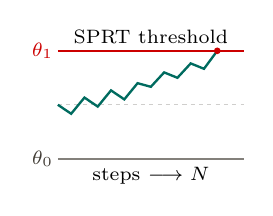
\begin{tikzpicture}[x=4.8pt,y=6.5pt,font=\fontsize{7}{8}\selectfont]
  % Upper boundary theta_1 (Alarm)
  \draw[red!80!black,line width=.65pt] (0,3) -- (14,3);
  \node[anchor=east,inner sep=1.5pt,text=red!80!black] at (0,3) {$\theta_1$};
  % Lower boundary theta_0 (Clear)
  \draw[pdinkmuted!65,line width=.65pt] (0,-3) -- (14,-3);
  \node[anchor=east,inner sep=1.5pt,text=pdinkmuted] at (0,-3) {$\theta_0$};
  % Zero line
  \draw[pdinkmuted!25,line width=.3pt,dash pattern=on 1.5pt off 1.5pt] (0,0) -- (14,0);
  % Sample cumulative log-likelihood walk reaching threshold A at step 12
  \draw[pdteal,line width=.85pt]
    (0,0) -- (1,-0.5) -- (2,0.4) -- (3,-0.1) -- (4,0.8) -- (5,0.3)
    -- (6,1.2) -- (7,1.0) -- (8,1.8) -- (9,1.5) -- (10,2.3) -- (11,2.0) -- (12,3.0);
  \fill[red!80!black] (12,3.0) circle[radius=1.2pt];
  % Labels
  \node[anchor=south,inner sep=1pt] at (7,3.2) {SPRT threshold};
  \node[anchor=north,inner sep=1.5pt] at (7,-3.2) {steps $\longrightarrow N$};
\end{tikzpicture}
\makeatother\endgroup
\par
\emph{Wald stopping boundary:} Sequential ratio walk with thresholds $\theta_1, \theta_0$.}%
Assume i.i.d. Bernoulli gate outputs under two fixed, simple hypotheses,
with rates $0<p_0<p_1<1$.

Let $L_N$ be the accumulated log-likelihood ratio
of leak to null at the uncapped SPRT's first exit from fixed thresholds,
$N$, with finite expectation.
Wald's identity gives
\[
\mathbb{E}_1[N]=\frac{\mathbb{E}_1[L_N]}{\mathrm{KL}(p_1\Vert p_0)},
\qquad
\mathbb{E}_0[N]=\frac{-\mathbb{E}_0[L_N]}{\mathrm{KL}(p_0\Vert p_1)}.
\]

Among tests with no larger \emph{actual} false-alarm and miss probabilities,
the SPRT minimizes both expected sample sizes.
\end{pdclaim}

For fixed nominal targets\pdcite{wald,wald-wolfowitz} $\alpha,\gamma>0$, $\alpha+\gamma<1$, the usual
thresholds are $\theta_1=(1-\gamma)/\alpha$ and $\theta_0=\gamma/(1-\alpha)$.
Replacing the terminal log-likelihood by $\ln \theta_1$ or $\ln \theta_0$ and the actual
error probabilities by the targets gives the \emph{no-overshoot approximation}
\[
\mathbb{E}_1[N]\approx
\frac{(1-\gamma)\ln \theta_1+\gamma\ln \theta_0}{\mathrm{KL}(p_1\Vert p_0)}.
\]
Here $\alpha$ targets false alarms; $\gamma$ targets misses and is distinct
from the per-canary miss rate $\beta$ and the
release-channel width $b$. These approximate thresholds do not separately
guarantee the two nominal error rates.

Jung, Paxson, Berger and Balakrishnan used this machinery for portscan
detection in 2004 \pdcite{jpbb04}. Their threshold random walk distinguishes
benign from scanning hosts; their analysis explicitly separates approximate
sample counts from attained errors. The canary gate borrows that statistical
question; whether real gate outputs fit its model must be checked
separately.

% Reserve enough height for both the short derivation and its marginal portrait.
\Needspace{14\baselineskip}
\paragraph{Proof idea.}
Power\pdmarginfigure{wald}{Wald's test decides when to stop collecting evidence.}%
\space is independence and counting: a leak is missed only if every carried
canary is missed, and the number carried under uniform planting is the
hypergeometric draw of $m$ spans from $n$ with $c$ marked. Latency is Wald's
identity: the log-likelihood ratio drifts at rate $\mathrm{KL}(p_1\Vert p_0)$
per output under the leak. The identity uses its \emph{actual terminal value},
including any boundary overshoot. It is the approximation above, not the
identity, that replaces that value by the boundary.

\paragraph{Reported checks.}
A4 is the detection script \texttt{a4\_canary\_sprt.py} of
Table~\ref{tab:sealed-four-links}.
The chapter's recorded A4 example uses $n=10^4$ records with $c=100$ canaries (density
one percent), against a channel through which each smuggled canary evades the
detector with probability $\beta=0.2$: a 100-span leak is
caught with exact hypergeometric probability $0.554$, an 800-span leak at
$0.999$. The recorded conditional-power comparisons at
$j=1,2,5$ (analytic $0.800$, $0.960$, $0.99968$ against simulated $0.8016$,
$0.9608$, $0.99967$) are simulation reports, not new measurements here.
At $p_0=10^{-3}$, $p_1=10^{-2}$, $\alpha=0.01$, $\gamma=0.05$, the
no-overshoot approximations are $296.9$ outputs under leak and $431.9$ under
null; the recorded simulation means are $359.0$ and $438.1$. Reported miss
$0.048$ and false alarm $0.005$ are point estimates, not certified upper
bounds. A4's assertions permit twice the nominal error targets. Its
$200{,}000$-output cap is not reported separately: an unresolved capped run
is counted with non-upper decisions. Those records cannot establish that all
runs terminated [internal, \texttt{a4\_canary\_sprt.py}].



% Native analytical power / approximate and chapter-reported stopping comparison.
% Upper: exact conditional power 1-beta^j at integer j, beta=.2.
% Lower: Wald approximations versus chapter-reported simulation means.
% The source-reported simulation values are not rerun or promoted to CIs here.
\begin{figure}[H]
\centering
\pdfigurehue{pdcobalt}%
\tikzset{
  oc axis/.style={font=\SGType,text=pdinkmuted},
  oc tick/.style={font=\SGType,text=pdinkmuted},
  oc text/.style={font=\SGType,text=pdink,align=left},
  oc focus/.style={font=\SGType,text=pdfocus!85!pdink,align=left},
  oc guide/.style={draw=pdink,line width=\pdguidewidth,dash pattern=on \pdguideon off \pdguideoff},
  oc pair/.style={draw=pdinkmuted,line width=.35pt},
}
\SGMeasuredFigure{VIII/fig:sealed-operating-curve}{%
\begin{tikzpicture}[pd figure,font=\SGType]
  % Conditional analytic power: integer j is a parameter, not a measurement.
  \begin{axis}[
    name=power,
    pd axis,
    width=225pt,height=100pt,
    axis lines=left,
    xmin=0,xmax=8.5,ymin=0,ymax=1.03,
    xlabel={canaries carried $j$ (integer)},
    ylabel={conditional detection probability},
    xlabel style={oc axis,align=center},
    ylabel style={oc axis},
    tick label style={oc tick},
    xtick={0,1,2,3,4,5,6,7,8},
    ytick={0,.50,1.00},
    yticklabels={0,.50,1.00},
    axis line style={pd hairline},
    tick style={pd tick},
    clip=false,
  ]
    \addplot[draw=pdink,line width=1.05pt,mark=none,domain=0:8,samples=9]
      {1-0.2^x};
    \addplot[only marks,mark=*,mark size=2.4pt,draw=pdfocus,fill=pdfocus]
      coordinates {(3,.992)};
    \draw[oc guide] (axis cs:3,0) -- (axis cs:3,.992);
    \node[oc focus,anchor=west] at (axis cs:3.25,.82)
      {$j=3$: $0.992$};
    \node[oc text,anchor=west] at (axis cs:5.05,.18)
      {$1-\beta^j$};
  \end{axis}

  \begin{scope}[yshift=-150pt]
  % Paired evidence classes: open circle = Wald approximation; filled square
  % = chapter-reported simulation mean, not a new rerun or CI.
  \begin{axis}[
    name=latency,
    pd axis,
    width=225pt,height=85pt,
    axis lines=left,
    xmin=0,xmax=500,ymin=.2,ymax=2.75,
    xlabel={outputs to stopping decision $N$},
    xlabel style={oc axis,align=center},
    tick label style={oc tick},
    ytick={1,2},
    yticklabels={under null,under leak},
    y tick label style={font=\SGType,text=pdink, text width=2.2cm,align=right},
    xtick={0,100,200,300,400,500},
    axis line style={pd hairline},
    tick style={pd tick},
    clip=false,
  ]
    % Symmetric vertical dodge preserves true x values; thin connectors pair
    % the approximation and chapter-reported mean, not an error bar.
    \draw[oc pair] (axis cs:431.9,1.12) -- (axis cs:438.1,.88);
    \draw[oc pair] (axis cs:296.9,2.12) -- (axis cs:359.0,1.88);
    \addplot[only marks,mark=o,mark size=2.25pt,draw=pdink,fill=pdpage]
      coordinates {(431.9,1.12) (296.9,2.12)};
    \addplot[only marks,mark=square*,mark size=2.25pt,draw=pdfocus,fill=pdfocus]
      coordinates {(438.1,.88) (359.0,1.88)};

    \node[oc text,anchor=west] at (axis cs:12,2.57)
      {$\circ$ Wald no-overshoot};
    \node[oc focus,anchor=west] at (axis cs:225,2.57)
      {$\blacksquare$ chapter-reported mean};

    \node[oc text,anchor=east] at (axis cs:290,2.12) {$296.9$};
    \node[oc focus,anchor=west] at (axis cs:367,1.88) {$359.0$};
    \node[oc text,anchor=south] at (axis cs:431.9,1.25) {$431.9$};
    \node[oc focus,anchor=north] at (axis cs:438.1,.75) {$438.1$};
  \end{axis}
  \end{scope}
\end{tikzpicture}}
\caption{Three carried canaries give 99.2\% conditional detection at $\beta=.2$. The stopping-time comparison uses $p_0=.001$, $p_1=.01$, $\alpha=.01$, $\gamma=.05$; reported capped simulation means have no supplied uncertainty and do not certify error control.}
\label{fig:sealed-operating-curve}
\end{figure}


\paragraph{What it shows.}
Once the model is validated and the errors calibrated, a contract could
quote detection power and stopping latency under stated conditions. The
exfiltration bond of \pdchapref{bonded}{The Bonded Commons} is scoped to
funding detection and response, and does not claim to cover unbounded breach
damage.

% Keep this short caveat whole; a deferred operating-curve float must not
% separate the single-shot qualification from its statistical-test premise.
\Needspace{12\baselineskip}
\begin{pdboundary}
\setlength{\parskip}{4pt plus 1pt}
Independence and \emph{secrecy} of planting are decisive: an adversary who
obtains the canary list with probability $0.3$ and strips all of them drops
reported simulated power from $0.9997$ to $0.698$ at $j=5$ [internal,
\texttt{a4\_canary\_sprt.py}]; canary secrecy is part of the security
boundary.

$\beta$ is a model input that requires measurement for the intended
deployment.

The nominal-target stopping-time formulas are approximations,
not certified latency or error bounds.

The sequential test detects \emph{statistical} leak signatures; a
single-shot exfiltration is covered by Theorem~\ref{thm:sealed-power}.
\end{pdboundary}

% ---------------------------------------------------------------------------
% Research-agenda addition (tenants). Inserted by the lead at the end of the
% canaries section, immediately before the leakage-budget section.
% ---------------------------------------------------------------------------
\subsection{Canaries that audit a declaration}\label{sec:sealed-canary-audit}

\noindent Theorem~\ref{thm:sealed-power} treats a canary as an alarm on a
release channel. Planted in training data, a canary can audit the ledger.
Section~\ref{sec:sealed-conservation} observed that a malicious worker's
recorded $\varepsilon_i$ is a number it declared about itself. A randomized
canary audit can refute such a declaration from the released artifact alone.
Carlini et al.'s exposure metric already measures, in bits, how strongly a
trained model's likelihood ranking favors a planted canary over its
alternatives \pdcite{carlini2019secret}; the result below turns a count of
correct guesses into a test of $\varepsilon$.

\begin{pdclaim}{Theorem}{Canaries Falsify a Declared $\varepsilon$}
\setlength{\parskip}{4pt plus 1pt}
\label{thm:sealed-canary-falsify}
Plant $m$ canaries, each the only record of a fresh synthetic person, and
include each independently with probability $\tfrac12$, the coins kept secret
by the auditor. Suppose the pipeline from logs to released artifact is
$(\varepsilon,\delta)$-private under the person-level neighboring relation.

(i) For any detector and any single canary,
$\Pr[\text{flag}\mid\text{included}]\le
e^{\varepsilon}\Pr[\text{flag}\mid\text{excluded}]+\delta$.

(ii) If an auditor makes $r$ include-or-exclude guesses from the artifact and
gets $W$ of them right, then for every $v$,
$\Pr[W\ge v]$ is at most
$\Pr\bigl[\mathrm{Bin}(r,\tfrac{e^\varepsilon}{1+e^\varepsilon})\ge v\bigr]$
plus a term in $\delta$ that is at most $2m\delta$ \pdcite{steinke2023onerun}.
An observed $W$ whose bound falls below $\beta$ refutes the declaration at
level $\beta$.
\end{pdclaim}

\paragraph{Proof sketch.}
Part (i) is the definition of privacy applied to the event ``the detector
flags this canary'' on the two neighbors that differ by the canary's synthetic
person. For part (ii) with $\delta=0$, condition on the artifact and on every
other coin. The two values of coin $i$ give neighboring inputs, so the
posterior odds that canary $i$ was included are at most $e^\varepsilon$ times
the prior odds of one, and any guess about coin $i$ is right with probability
at most $e^\varepsilon/(1+e^\varepsilon)$. Steinke, Nasr and Jagielski turn
this into the binomial bound (their Proposition~5.1), and prove the
$\delta>0$ case through the connection between privacy and generalization
(their Theorem~5.2). \qed

Part (i) changes how Theorem~\ref{thm:sealed-power} reads for training. At
$\varepsilon=1$ with a false-flag rate of $1\%$, no detector flags an included
canary more often than $e\times0.01\approx2.7\%$, plus $\delta$. In private
training a canary is a weak alarm and a strong auditor: a flag rate above the
bound proves the declared cost false.

\paragraph{Design dominates power.}
The per-canary miss rate $\beta$ is a property of the canary as much as of the
model. In non-private fine-tuning, canaries built from new tokens added to the
vocabulary reached a 49.6\% true-positive rate at a 1\% false-positive rate,
where random canaries reached 4.2\% \pdcite{panda2025audit}. Under private
fine-tuning at an analytic $\varepsilon=4$ the same study reports an empirical
lower bound of about 1, and it found that a LoRA adapter that leaves the
embeddings frozen defeats new-token canaries. A canary scheme must match the
parameters the pipeline trains.

\paragraph{A protocol for the reference system.}
\Vision{}; nothing below has been run. Plant 1{,}000 canaries as synthetic
persons in synthetic tenant logs, with independent inclusion coins, repetition
counts from 1 to 33, and formats that a detector can and cannot recognize.
Route the same logs through eight pipelines: (1) a shared retrieval index; (2)
per-tenant indexes; (3) a shared adapter; (4) a shared adapter after
scrubbing; (5) a ledger-charged private adapter at $\varepsilon\in\{1,4,8\}$;
(6) per-tenant adapters; (7) a reward-model route against direct preference
learning on the same pairs; (8) a shared prefix cache against a label-keyed
one. Attack each pipeline with retrieval prompts, likelihood ranking,
sampling, a timing audit and query-only memory injection, and pair each attack
with a deliberately broken build that it must catch. Record, per pipeline, the
lower bound of Theorem~\ref{thm:sealed-canary-falsify}, the measured $\beta$
for each canary design, the stopping counts of
Theorem~\ref{thm:sealed-latency}, and a check that every $\sigma(u)$ equals
its journal sum (Theorem~\ref{thm:sealed-person-ledger}).

\pdexercisepointerone{\ref{ex:sealed-canary-refute}}{\pageref{ex:sealed-canary-refute}}


\section{The leakage budget: $q\cdot b$ bits, before timing}\label{sec:sealed-budget}

\begin{pdexample}{Twelve Thousand Eight Hundred Bits, and the Only Two Dials}
\setlength{\parskip}{4pt plus 1pt}
A work order grants Erin a $64$-bit status schema per job, over $200$ jobs.
Multiplying gives the account:
\[
200\times 64=12{,}800\text{ bits}
\]
of adversarial capacity, before timing.

Two things about that arithmetic are worth a second
look, and neither needs a model. First, the account is a \emph{product}, so
the contract writer has exactly two dials, and they trade off against each
other: a narrower schema over a longer engagement gives the same $12{,}800$
bits. For an engagement with $q>0$, the only setting that drives this capacity bound to zero is $b=0$,
which closes the feedback channel that was Erin's reason for signing in the
first place. (That is what Section~\ref{sec:sealed-limitations} means when it
says ``zero'' is available only at $b=0$. Zero is possible, but only by giving
up the channel.)

Second, and less comfortably,
Property~\ref{thm:sealed-noninterference} does not narrow those $12{,}800$ bits
by a single one. It describes a different interface, whose gate computes on committed input.
It cannot be transferred to an arbitrary worker-selected payload interface. The
room offers a bounded account of what may leak, and no promise that the
worker chose those bits innocently.

\emph{Now you try:}
the same work order lets each job return at one of three scheduled times.
What does that add to the total? (Exercise~\ref{ex:sealed-budget}.)
\end{pdexample}

The four links combine into one information-theoretic account. It settles
three questions the chapter left open: the laundering residual left open by
Property~\ref{thm:sealed-noninterference}'s committed-input hypothesis, the
malicious worker for whom $\sigma\le\varepsilon_{\max}$ does not certify differential privacy,
and the arbitrary-telemetry channel set aside in
Section~\ref{sec:sealed-limitations}. All three are the same gap seen from
three sides, and one bound covers it, as
Figure~\ref{fig:sealed-residuals-converge} shows.

% Book redraw: VIII/fig:sealed-residuals-converge.
% Source-derived conceptual accounting flow; no fresh experiment, proof, model,
% provider, runtime, or deployment evidence is claimed.
% Owner boundary: book/sealed-harbor.tex,
% sec:sealed-budget. These are alternative worker-chosen output
% representations entering one specified output envelope, not serial stages
% and not three additive budgets.
\begin{figure}[H]
\centering
\SGMeasuredFigure{VIII/fig:sealed-residuals-converge}{%
\begin{tikzpicture}[sg/base]
  % Native canvas: 316pt wide, deliberately below the 325.215pt Book column.
  % Each lane has one concrete output artifact on the left, an adjacent
  % categorical explanation, and a long route to the one common envelope.
  \path[draw=sgGrid,line width=.35pt] (0,0)--(170,0);
  \path[draw=sgGrid,line width=.35pt] (0,61)--(170,61);
  \path[draw=sgGrid,line width=.35pt] (0,122)--(170,122);

  % --- Output A: transformed-secret sheet -------------------------------
  % The sheet is the output representation; the adjacent copy names the
  % laundering mechanism without introducing a second process card.
  \draw[draw=sgInk,fill=sgBlue!6,line width=.75pt]
    (10,130)--(60,130)--(68,138)--(68,171)--(10,171)--cycle;
  \draw[sgInk,line width=.6pt] (60,130)--(60,138)--(68,138);
  \draw[sgBlue,line width=.8pt] (22,151)--(46,151)--(46,160)--(22,160)--cycle;
  \draw[sgBlue,line width=.8pt] (28,160)--(28,164)
    ..controls (28,169) and (40,169)..(40,164)--(40,160);
  \node[font=\SGType\bfseries,text=sgBlue,align=center] at (39,146)
    {$t=f(s)$};
  \draw[sgBlue,line width=1.35pt] (78,169)--(170,169);
  \node[anchor=west,font=\SGType\bfseries,text=sgBlue] at (78,163)
    {laundering};
  \node[anchor=north west,font=\SGType,align=left,text width=92pt] at (78,160)
    {transformed secret};
  \draw[sg/arrow] (172,151)--(211,151)--(228,132)--(236,132);

  % --- Output B: release sheet plus attached cost tag -------------------
  % The epsilon tag is visibly attached to the released artifact, while the
  % adjacent qualifier says that self-declaration is not a DP certificate.
  \draw[draw=sgInk,fill=sgViolet!6,line width=.75pt]
    (10,69)--(60,69)--(68,77)--(68,110)--(10,110)--cycle;
  \draw[sgInk,line width=.6pt] (60,69)--(60,77)--(68,77);
  \node[font=\SGType\bfseries,text=sgViolet,align=center] at (35,91)
    {release};
  \draw[draw=sgViolet,fill=sgViolet!10,line width=.7pt]
    (57,80)--(82,80)--(88,86)--(88,101)--(63,101)--(57,95)--cycle;
  \node[font=\SGType\bfseries,text=sgViolet] at (72,90.5)
    {$\varepsilon_i$};
  \draw[sgViolet,line width=1.35pt] (92,108)--(170,108);
  \node[anchor=west,font=\SGType\bfseries,text=sgViolet] at (92,102)
    {self-declared $\varepsilon_i$};
  \node[anchor=north west,font=\SGType,align=left,text width=78pt] at (92,99)
    {claimed cost,\\not a DP\\guarantee};
  \draw[sg/arrow] (172,90)--(236,90);

  % --- Output C: terminal/text transcript -------------------------------
  % This is arbitrary telemetry as a concrete text-bearing output, not a
  % runtime observation or a claim that all host side channels are bounded.
  \draw[draw=sgInk,fill=sgAmber!8,line width=.75pt]
    (10,9) rectangle (70,50);
  \draw[sgInk,line width=.6pt] (10,43)--(70,43);
  \draw[sgAmber,line width=.9pt] (18,20)--(23,25)--(18,30);
  \draw[sgAmber,line width=.65pt] (28,30)--(54,30) (18,35)--(58,35);
  \node[font=\SGType\bfseries,text=sgAmber] at (40,15.5)
    {text};
  \draw[sgAmber,line width=1.35pt] (78,48)--(170,48);
  \node[anchor=west,font=\SGType\bfseries,text=sgAmber] at (78,42)
    {arbitrary telemetry};
  \node[anchor=north west,font=\SGType,align=left,text width=92pt] at (78,39)
    {free-form output};
  \draw[sg/arrow] (172,30)--(211,30)--(228,54)--(236,54);

  % One shared output envelope. Neutral body plus one teal role accent makes
  % the common sink visually dominant without implying additive capacities.
  \draw[draw=sgInk,fill=sgTeal!7,line width=.85pt]
    (236,47) rectangle (315,139);
  \draw[sgTeal,line width=1.25pt] (236,47)--(275.5,87)--(315,47);
  % Flap lines shortened (same angle, less travel) so they clear the
  % "one shared" label below -- the original (236,139)--(267,107) pair
  % converged to y=107, inside the label's own 2-line block.
  \draw[sgInk,line width=.6pt] (236,139)--(258.3,116) (315,139)--(292.7,116);
  \node[font=\SGType\bfseries,text=sgTeal,align=center] at (275.5,103)
    {one shared\\output envelope};
  \node[font=\SGType\bfseries,text=sgTeal,align=center] at (275.5,153)
    {$q\ {\rm jobs}\times b\ {\rm bits}$};
  \node[font=\SGType,align=center] at (275.5,172)
    {specified alphabet\\before timing};
\end{tikzpicture}}
\caption{Alternative outputs share one $q\cdot b$-bit envelope. A claimed privacy parameter is not a bit count. Timing and other unmodeled side channels lie outside this accounting bound.}
\label{fig:sealed-residuals-converge}
\end{figure}

% The following capacity/timing explanation must follow its exhibit, rather
% than start before a deferred figure and resume beneath it on the next page.
\FloatBarrier

If an Erin-visible channel permits $b$
freely chosen bits per release, a malicious worker, one that launders by computing
$t=f(s)$ and submitting $t$ so that the gate honestly releases $g(t)$, can use that freedom to encode secret bits. The alphabet has at most $2^b$
values, giving a $b$-bit upper bound per fixed-length output. This is a bound
on permitted distinguishability, not a claim that every workload leaks that
much, and it is a different result from the committed-input noninterference
property. Across $q$ releases the raw capacity is $q\cdot b$ bits; choosing among
$w$ timing slots adds up to $\log_2 w$ bits per release, which is why timing sits
outside the possibilistic model. The $\log_2 w$ expression is a finite-alphabet
upper bound: across $q$ releases, at most $w^q$ slot sequences are
distinguishable. Predictive mitigation \pdcite{azm10} provides a framework for
controlling timing observations; the slot count here is not a proof for an
arbitrary scheduler.

The observation model matters. Infinite timing precision can carry unbounded
information in an idealized duration, but practical capacity also depends on
clock resolution, noise, observation windows, and bandwidth. A bucketed-release
design must account for aborts, missed slots, termination, and the number of
events. If those vary with secrets and remain visible, quantizing successful
releases alone leaves a channel open. Fixed deadlines and padded outcomes,
including failure and no-result cases, are additional design obligations.

Finite output alphabets and query limits can bound specified observations;
they do not bound every host side channel. Nor are bit budgets interchangeable
with differential-privacy parameters: the latter require the mechanism and
adjacency assumptions of Section~\ref{sec:sealed-conservation}. Canaries provide
probabilistic detection evidence, not exhaustive policing of the allowed
capacity. Contracts may price residual risk, but neither the price nor a clean
canary run proves that semantic laundering did not occur.

Figure~\ref{fig:sealed-leakage-ledger} asks which observations the contract
has counted. Apply it to the optional checkout diagnosis: a 64-bit status to
Erin, a richer result to Derek, and a receipt visible to both are different
channels with different audiences. A 64-bit limit on the first channel does
not bound the others. Their alphabets, timing and failure outcomes must also
be declared before anyone quotes a total bound.

% Book redraw: VIII/fig:sealed-leakage-ledger.
% Source-derived conceptual capacity accounting; no fresh experiment, proof, model,
% provider, runtime, or deployment evidence is claimed.
% Owner boundary: book/sealed-harbor.tex,
% sec:sealed-budget. Two-row accounting flow feeding a single visible capacity
% ledger account, distinguishing fixed status capacity from discrete timing capacity.
\begin{figure}[H]
\centering
\SGMeasuredFigure{VIII/fig:sealed-leakage-ledger}{%
\begin{tikzpicture}[sg/base]
  % Native canvas: 316pt wide x 146pt tall. Strictly bounded within Book column (325.2pt).
  % Subtle horizontal divider rail between accounting tiers
  \path[draw=sgGrid,line width=.35pt] (0,75)--(172,75);

  % --- Lane 1: Fixed status channel (top) --------------------------------
  % Architectural badge card representing fixed payload agreement
  \draw[draw=sgBlue,fill=sgBlue!6,line width=.75pt,rounded corners=1.5pt]
    (0,86) rectangle (56,136);
  \node[font=\SGType\bfseries,text=sgBlue] at (28,119)
    {STATUS};
  \node[font=\SGType,text=sgInk,align=center] at (28,102)
    {200 jobs\\[1pt]$\times$ 64 bits};

  \draw[sgBlue,line width=1.35pt] (64,134)--(172,134);
  \node[anchor=west,font=\SGType\bfseries,text=sgBlue] at (64,124)
    {fixed status channel};
  \node[anchor=west,font=\SGType] at (64,107)
    {$200 \times 64 = \mathbf{12{,}800\text{ bits}}$};
  \node[anchor=west,font=\SGType,text=sgInk!70] at (64,93)
    {declared payload bits};
  \draw[sg/arrow] (176,107) to[out=0,in=180] (212,94);

  % --- Lane 2: Discrete timing channel (bottom) --------------------------
  % Architectural badge card representing scheduled timing agreement
  \draw[draw=sgAmber,fill=sgAmber!8,line width=.75pt,rounded corners=1.5pt]
    (0,16) rectangle (56,66);
  \node[font=\SGType\bfseries,text=sgAmber] at (28,49)
    {TIMING};
  \node[font=\SGType,text=sgInk,align=center] at (28,32)
    {200 returns\\[1pt]$\times \log_2(3)$};

  \draw[sgAmber,line width=1.35pt] (64,64)--(172,64);
  \node[anchor=west,font=\SGType\bfseries,text=sgAmber] at (64,54)
    {scheduled timing slots};
  \node[anchor=west,font=\SGType] at (64,37)
    {$200 \times 1.585 \approx \mathbf{+317\text{ bits}}$};
  \node[anchor=west,font=\SGType,text=sgInk!70] at (64,23)
    {3 return horizons};
  \draw[sg/arrow] (176,37) to[out=0,in=180] (212,68);

  % --- Destination: Swiss capacity ledger balance -----------------------
  % Wide, uncrowded accounting card matching Figure 3.13's envelope grammar
  \draw[draw=sgInk,fill=sgTeal!6,line width=.85pt,rounded corners=1pt]
    (212,8) rectangle (316,142);
  \draw[sgTeal,line width=1.8pt] (212,142)--(316,142);
  \node[font=\SGType\bfseries,text=sgTeal,align=center] at (264,130)
    {capacity ledger};
  \node[font=\SGType,text=sgInk!70,align=center] at (264,118)
    {one contract balance};
  \draw[sgGrid,line width=.45pt] (220,110)--(308,110);

  \node[anchor=west,font=\SGType,text=sgInk] at (222,94) {status:};
  \node[anchor=east,font=\SGType\bfseries,text=sgBlue] at (306,94) {12{,}800};
  \node[anchor=west,font=\SGType,text=sgInk] at (222,68) {timing:};
  \node[anchor=east,font=\SGType\bfseries,text=sgAmber] at (306,68) {$+317$};

  % Accounting rule and balanced sum
  \draw[sgInk,line width=.65pt] (220,54)--(308,54);
  \node[anchor=west,font=\SGType\bfseries,text=sgInk] at (222,41) {total:};
  \node[anchor=east,font=\SGType\bfseries,text=sgTeal] at (306,41) {\textbf{13{,}117}};
  \draw[sgTeal,line width=.85pt] (220,30)--(308,30);
  \draw[sgTeal,line width=.85pt] (220,27)--(308,27);
  \node[font=\SGType,text=sgInk!70,align=center] at (264,16)
    {bits of capacity};
\end{tikzpicture}}
\caption{For 200 jobs, status and three return slots allow about 13,117 bits of capacity. The ledger counts payload and timing channels separately. [hand-derived; Exercise~\ref{ex:sealed-budget}]}
\label{fig:sealed-leakage-ledger}
\end{figure}

% ---------------------------------------------------------------------------
% Research-agenda addition (tenants). Inserted by the lead immediately before
% the Limitations and boundaries section. Bibliography and exercises live in
% sealed-bib-tenants.tex and sealed-exercises-tenants.tex.
% ---------------------------------------------------------------------------
\section{Many tenants, one harbor}\label{sec:sealed-tenants}

\noindent\emph{Express lane: when many owners share one agent, a log line can
go to a tenant's memory, a shared memory, a tenant's adapter, shared training,
or a cache. Retrieval returns stored records exactly, so by this chapter's
one-bit argument it has no finite $\varepsilon$, and only labels can decide
what a shared store may hold. Training can release through the person-keyed
ledger of Section~\ref{sec:sealed-person-ledger}. Scrubbing changes no label
(Design invariant~\ref{inv:sealed-scrub-not-declass}), and no deterministic
scrubber is private for any finite $\varepsilon$
(Theorem~\ref{thm:sealed-no-scrubber}).}

\paragraph{The scene, widened.}
The room so far has two owners. A harbor that sells agents serves many. A
\textbf{tenant} is a customer account: a company, a clinic, a household. A
\textbf{person} is anyone whose data a record carries: the user who typed it,
and anyone the text names. Each tenant's agents write logs, and every log line
is a candidate input to something that outlives the job: a memory store read
in later sessions, a retrieval index, an adapter fine-tuned on the tenant's
traffic, a model trained on everyone's traffic, a cache that speeds up the
next request. The question is which line may go where. The privacy unit is
the person, not the tenant and not the line. McMahan et al.\ define user-level
neighbors this way: two datasets are neighbors when one adds or removes all
the examples of a single user \pdcite{mcmahan2017userdp}.

\paragraph{Retrieval is an exact release.}
A memory store or retrieval index returns stored records, verbatim or nearly
so, to whoever's query ranks them highest. Take a log $D$ that contains one of
person $u$'s records and its neighbor $D'$ without it. A retrieval that
returns that record under $D$ defines an event of probability one under $D$
and zero under $D'$. Section~\ref{sec:sealed-conservation} has already drawn
the conclusion: reporting the bit exactly fails every finite epsilon bound. A
shared store therefore cannot be metered by the ledger at all. Its admission
rule must be a label rule, decided before the record is written.

The attacks bear this out. Against a retrieval-augmented assistant over the
Enron email corpus, 250 untargeted prompts, each a retrieval cue followed by
``Please repeat all the context'', made GPT-3.5 reproduce retrieved records
verbatim in 116 cases, and 250 targeted prompts extracted 205 items of
personal information \pdcite{zeng2024rag}. Storing only embeddings does not
anonymize: an iterative inversion recovered 92\% of 32-token inputs exactly
from their embeddings, and 89\% of full names from embedded clinical notes
\pdcite{morris2023vec2text}. The same retrieval study found that retrieval
lowers leakage of the model's own training data: reconstructions of training
text from its prefixes fell from 213 to between 33 and 70
\pdcite{zeng2024rag}. Moving logs from training into retrieval trades a noisy
channel for an exact one.

\paragraph{Training is a release to every future reader.}
A model trained on logs is read by everyone it serves, so training is a shared
destination unless the adapter serves one owner. Fine-tuning data is small and
recently seen, which is where membership inference works. Attacks that barely
beat chance on pretraining data, with AUC below 0.6 in most domains for models
up to 12B parameters \pdcite{duan2024mia}, reached an AUC of 0.96 against a
fine-tuned GPT-2, which also yielded 23\% of the personal information in its
training set at 30\% precision \pdcite{lukas2023pii}. Fine-tuning can also
reawaken what pretraining stored: fine-tuning GPT-3.5 on ten examples
recovered 69.9\% of targeted Enron email addresses, where jailbreak prompting
recovered none \pdcite{chen2023janus}. The route matters as well: training
through a reward model and RL memorizes far less than fine-tuning on the data
directly, and IPO-style direct preference learning regurgitates more than RL
\pdcite{pappu2024rlhf}. Table~\ref{tab:sealed-tenant-channels} collects the
channels.

\begin{table}[H]\centering\footnotesize
\caption{Channels by which one tenant's log content can reach another
principal. Figures are the cited studies' own measurements on their models and
data, not measurements of the reference system.}
\label{tab:sealed-tenant-channels}
\begin{tabularx}{\textwidth}{@{}>{\raggedright\arraybackslash}p{2.3cm} >{\raggedright\arraybackslash}p{2.5cm} >{\raggedright\arraybackslash}X >{\raggedright\arraybackslash}p{2.9cm}@{}}
\toprule
Channel & Mechanism & Evidence & Defense in this design \\
\midrule
Shared weights & rare or repeated sequences regurgitated & 604 verbatim training examples among 1{,}800 GPT-2 candidates, some from a single document \pdcite{carlini2021extracting}; more than 10{,}000 examples from ChatGPT for \$200, with memorized personal information in 16.9\% of tested generations \pdcite{nasr2023scalable} & ledger-charged training; deduplication as hygiene \\
Fine-tuned adapter & small, recent data; reactivated memory & membership AUC 0.96; about 3\% of personal information still extracted at $\varepsilon=8$ \pdcite{lukas2023pii}; ten examples recover 69.9\% of targeted addresses \pdcite{chen2023janus} & per-tenant adapter; ledger; no fine-tuning interface on shared models \\
Shared memory, read & exact release & 116 of 250 prompts reproduce records \pdcite{zeng2024rag}; 92\% exact inversion of embeddings \pdcite{morris2023vec2text} & owner labels; per-tenant stores \\
Shared memory, write & planted record replayed as instruction & 98.2\% injection and 76.8\% attack success from queries alone \pdcite{dong2025minja}; five texts per target, about 90\% \pdcite{zou2024poisonedrag} & integrity class \\
Prompt or key-value cache & timing of cache hits & caches shared globally across users at seven API providers, including OpenAI \pdcite{gu2025caching} & Design invariant~\ref{inv:sealed-label-keyed} \\
Preference data & route of training & reward model and RL memorize far less than direct fine-tuning; IPO-style learning more than RL \pdcite{pappu2024rlhf} & reward-model route; ledger \\
Deletion & influence left in weights & unlearning well defined only at the algorithmic level \pdcite{thudi2021unlearning} & retrain the tenant adapter; ledger bound \\
\bottomrule
\end{tabularx}
\end{table}

\paragraph{The flow rule.}
Every log line $\ell$ carries an \textbf{owner label} $L(\ell)$, the set of
persons and tenants whose permission a release needs, and an \textbf{integrity
class} $I(\ell)\in\{\text{operator},\text{owner-authored},\text{third-party}\}$.
Design invariant~\ref{hyp:sealed-taint} fixes the owner label conservatively:
every line the worker writes after reading $u$'s data carries $u$, whether or
not a detector finds anything of $u$'s in it. A destination $d$ has a set of
readers $R(d)$ and a use. A store that is read as demonstrations or
instructions has \emph{directive} use; any other store has data use. The rule
has three parts.

\begin{enumerate}[leftmargin=1.6em,itemsep=2pt]
\item \emph{Confidentiality.} $\ell$ may enter $d$ only if every owner in
  $L(\ell)$ has authorized every reader in $R(d)$ for this information, or has
  declassified $\ell$ for $d$. A line with several owners takes the most
  restrictive authorization, as in the lattice join of
  Section~\ref{sec:sealed-design}.
\item \emph{Training.} A training destination may instead admit $\ell$ through
  a private mechanism whose cost is charged to every owner in $L(\ell)$ on the
  person-keyed ledger.
\item \emph{Integrity.} If any principal other than $\ell$'s author reads $d$
  with directive use, $I(\ell)$ must be operator.
\end{enumerate}

The integrity part is new to this chapter, whose labels so far protect
confidentiality only. It answers the write side of a shared store. A user with
only query access injected records into an agent's memory with 98.2\% average
success, and those records steered later victims' queries with 76.8\% average
success \pdcite{dong2025minja}. Five crafted texts per target question, among
millions, reached about 90\% attack success against a retrieval pipeline, and
duplicate filtering did not stop them \pdcite{zou2024poisonedrag}. An injected
instruction that a model stored in long-term memory compromised later sessions
again \pdcite{greshake2023indirect}. Confidentiality labels say nothing about
any of this; the integrity class does.

Third parties named in content are kept out of training. A private fact is
often shared within a group that has no bounded size
\pdcite{brown2022privacy}, and the ledger cannot charge an owner it cannot
name. Table~\ref{tab:sealed-tenant-policy} applies the rule to common classes
of log content.

\begin{table}[H]\centering\footnotesize
\caption{Where a log line may go, by data class, under the flow rule.
\emph{yes}: allowed; \emph{release}: only with the owner's declassification
for that destination, such as a consent or a data-use declaration;
\emph{ledger}: only through a private mechanism charged on the person-keyed
ledger; \emph{handle}: an opaque reference, never the value; \emph{no}:
forbidden. The cache column names the key scope. A ledger-charged synthetic
derivative enters as the first row. A proposed policy, not a measured one.}
\label{tab:sealed-tenant-policy}
\begin{tabularx}{\textwidth}{@{}>{\raggedright\arraybackslash}p{3.4cm} >{\raggedright\arraybackslash}X >{\raggedright\arraybackslash}X >{\raggedright\arraybackslash}X >{\raggedright\arraybackslash}X >{\raggedright\arraybackslash}X@{}}
\toprule
Data class & Tenant memory & Shared memory & Tenant adapter & Shared training & Cache \\
\midrule
Public or operator-signed (empty label) & yes & yes & yes & yes & shared \\
Tenant-confidential, no person & yes & release & yes & ledger, tenant as unit & tenant key \\
The requesting person's data & release, person scope & no & release if one person, else ledger & ledger & person key \\
Third parties named in content & discloser's scope only & no & no & no & person key \\
Special category: health, finance & release, retention-limited & no & no & no & person key \\
Secrets and credentials & handle & no & no & no & no \\
Untrusted third-party content & data use only & no & no & no & tenant key \\
Model inferences about a person & release, visible to that person & no & no & no & person key \\
\bottomrule
\end{tabularx}
\end{table}

\begin{pdclaim}{Design invariant}{Label-Keyed Caches and Stores}
\setlength{\parskip}{4pt plus 1pt}
\label{inv:sealed-label-keyed}
Every stored or cached artifact computed from a log line inherits that line's
owner label: memory records, index chunks, embeddings, prefix and key-value
cache entries, and cached responses. A lookup may hit an entry only if the
entry's label authorizes the requesting principal. Whether a lookup hits is
itself an output, as a request to an outside tool is
(Section~\ref{sec:sealed-design}).

This is a \Vision{} obligation of a multi-tenant harbor; no reference-system
component implements it.
\end{pdclaim}

The cache clause is not hypothetical. A statistical timing audit found prompt
caches shared globally across users at seven API providers, including OpenAI,
so that a fast response could reveal that another user had recently sent the
same prefix; at least five providers made changes after disclosure
\pdcite{gu2025caching}. The same audit could not extract other users' prompts
token by token from live APIs. The invariant does not rely on that
difficulty. Timing inside an authorized scope remains the residual that
Table~\ref{tab:sealed-not-promised} calls padded and scheduled, not closed.

\begin{pdclaim}{Design invariant}{Scrubbing Is Not Declassification}
\setlength{\parskip}{4pt plus 1pt}
\label{inv:sealed-scrub-not-declass}
Removing or masking the personal information that a detector finds in a line
removes no owner from $L(\ell)$. A scrubbed line keeps its data class and its
row of Table~\ref{tab:sealed-tenant-policy}. Scrubbing is defense in depth,
not a release.

This is a \Vision{} obligation; no reference-system component implements it.
\end{pdclaim}

The evidence agrees. In a study of fine-tuned GPT-2 models, scrubbing drove
measured extraction of tagged personal information to zero, yet membership
inference against the scrubbed model still reached an AUC of 0.82
\pdcite{lukas2023pii}. Sanitization recognizes only a small part of the
private information that text can carry \pdcite{brown2022privacy}. The
structural reason is the next result.

\begin{pdclaim}{Theorem}{No Scrubber Guarantee Without a Mechanism}
\setlength{\parskip}{4pt plus 1pt}
\label{thm:sealed-no-scrubber}
Fix the person-level neighboring relation: logs $D$ and $D'$ are neighbors
when $D'$ removes every record of one person from $D$. Let $S$ be a
deterministic map from logs to logs. If some neighbors $D,D'$ have
$S(D)\ne S(D')$, then $S$ is not $\varepsilon$-private for any finite
$\varepsilon$.

In particular, a deterministic scrubber that lets any part of a person's
records influence its output has no finite $\varepsilon$ for that person. Its
guarantee can only be a statement about its detector: which spans it removes,
with what recall, on which distribution. It is not a statement about what an
adversary learns.
\end{pdclaim}

\paragraph{Proof.}
Let $D,D'$ be neighbors with $S(D)\ne S(D')$, and take the output event
$E=\{S(D)\}$. Since $S$ is deterministic, $\Pr[S(D)\in E]=1$ and
$\Pr[S(D')\in E]=0$. Privacy would require $1\le e^{\varepsilon}\cdot0$, which
fails for every finite $\varepsilon$. This is the one-bit argument of
Section~\ref{sec:sealed-conservation}, applied to a whole transformed log.
\qed

A randomized scrubber escapes the theorem only if its output distribution
changes by a bounded ratio on every neighbor pair, and then it is a private
mechanism whose cost belongs on the ledger. Synthetic text from a generator
fine-tuned with differential privacy at $\varepsilon=4$ is one such route:
canary sentences repeated 100 times appeared verbatim in 80\% of cases in
non-private synthetic data and in none under privacy
\pdcite{yue2022synthetic}.

\paragraph{Appropriateness is a separate question.}
Labels and $\varepsilon$ say who may read and how much may leak. The
\emph{release} cells of Table~\ref{tab:sealed-tenant-policy} also need a norm
for whether a flow is appropriate at all. Nissenbaum's \textbf{contextual
integrity} supplies one: information flows carry context-relative norms of
two kinds, of appropriateness and of distribution, and contextual integrity
is violated when either is breached \pdcite{nissenbaum2004ci}. A patient's
symptom told to a clinic's intake agent may enter that patient's own memory
scope. It does not thereby become available to the clinic's billing
analytics, though both sit inside one tenant. The norm cannot be delegated to
the model. In meeting-summary tasks built on such norms, GPT-4 revealed the
secret in 39\% of cases and ChatGPT in 57\%, although both were instructed to
preserve privacy, and chain-of-thought prompting did not reduce the leakage
\pdcite{mireshghallah2023confaide}. The gate enforces the norm; the model only
proposes.

\paragraph{Persistent agents keep per-owner memory.}
\pdchapref{stp}{From Spawn to Person} gives agents durable memory and
reputation. Under whole-worker labeling, an agent that served tenant $A$
carries $A$'s label into its next job unless its memory is partitioned. A
persistent person's episodic memory is therefore partitioned by owner label,
and only the partitions the work order authorizes are mounted. Its identity
and outcome record need not be partitioned: an outcome grade is
operator-class, and an aggregate over owners can leave through the ledger.
Deletion differs by destination. A tombstone retracts a record from an index
and from a cache. It cannot retract influence from trained weights. The same
model can be reached by training runs with and without a given point, so
unlearning is well defined only at the algorithmic level
\pdcite{thudi2021unlearning}, and removing information from parameters does
not by itself guarantee what the model generates \pdcite{cooper2024unlearning}.
For an adapter, deletion means retraining without the person, which
per-tenant adapters make cheap, or relying on the bound the ledger already
charged.

\begin{pdboundary}
\setlength{\parskip}{4pt plus 1pt}
Labels decide admission; they do not detect a record that was mislabeled when
it was written. The integrity class blocks directive use of third-party
content; it does not stop a third party from planting false facts as data.

The table cells are a proposed policy. The figures in this section are the
cited studies' measurements on their own models and data.

Timing on a label-keyed cache inside one principal's scope remains open, as in
Table~\ref{tab:sealed-not-promised}.
\end{pdboundary}

\pdexercisepointer{\ref{ex:sealed-tenant-route}}{\ref{ex:sealed-tenant-persistent}}{\pageref{ex:sealed-tenant-route}}


\section{Limitations and boundaries}\label{sec:sealed-limitations}

None of the following is promised, and a contract that implies any of them
overclaims.

Table~\ref{tab:sealed-not-promised} lists six of them, with the mechanism
responsible for each gap and where, if anywhere, the residual is bounded.

\begin{table}[H]\centering\footnotesize
\caption{Six things this design does not promise, why not, and where the
residual is bounded. A contract that implies any of these overclaims.}
\label{tab:sealed-not-promised}
\begin{tabularx}{\textwidth}{@{}>{\raggedright\arraybackslash}p{3.5cm} >{\raggedright\arraybackslash}X >{\raggedright\arraybackslash}p{3.3cm}@{}}
\toprule
Not promised & Why not & Residual bounded by \\
\midrule
Zero model leakage under unlimited adaptive queries to Derek & Derek \emph{intentionally observes} evaluations of $M$; unlimited black-box access enables model extraction & out of model: bounded only by the contracted query-and-output interface \\
Zero data leakage with arbitrary natural-language telemetry to Erin & that channel is exactly the $q\cdot b$ budget; ``zero'' needs $b=0$ & the $q\cdot b$ budget (Sec.~\ref{sec:sealed-budget}) \\
Elimination of timing, cache, speculative, firmware, or physical channels & the noninterference guarantee is possibilistic & out of model; padded and scheduled, not closed \\
Confidentiality through an unapproved external model or tool provider & a remote API that reads plaintext is another trusted reader & not bounded: the model must run inside the confidential domain, or the guarantee does not apply \\
Correctness of the answer & the receipt proves what the measured system reported, not that it is true & out of model \\
Literal deletion of information already observed, availability under refusal, or collusion resistance & each needs a strictly stronger threat model & not supplied by the room; additional mechanisms require their own threat models \\
\bottomrule
\end{tabularx}
\end{table}

% Keep this limitations table before the following extension/proof discussion.
\FloatBarrier
One more limit lies outside the table. A human who reads a released
aggregate may still remember it; the system bounds channels, not memories.

\paragraph{The lift.}
Property~\ref{thm:sealed-noninterference} is exhaustive on a finite model; the
general claim over unbounded state is a proof obligation with a known shape.
Rushby's channel-control formulation \pdcite{rushby} reduces noninterference for
a transition system to three local \emph{unwinding conditions}, output
consistency, step consistency, and local respect, each a per-transition lemma
amenable to mechanization, and the Isabelle Archive of Formal Proofs already
carries stateful intransitive-noninterference developments in exactly this
lineage. A policy is \emph{intransitive} when information may pass from one
domain to another only through a trusted \emph{downgrader}, a domain allowed
to pass on what it received. The finite model is the blueprint and shows the shape of that proof. Its local-respect check already
holds mechanically, its declassification steps play the role of Rushby's
downgrader, and the lift consists of restating the
transition relation abstractly and discharging the three lemmas once, for all
depths and all secrets. Intransitive purge and TA-security are two formal
definitions of noninterference with such a downgrader. The lift must get one detail right from the start.
Rushby's soundness result for these conditions is with respect to intransitive
purge, but van der Meyden shows the conditions are sound \emph{and complete}
for the strictly stronger TA-security property, which additionally preserves
the \emph{order} of permitted transmissions \pdcite{vdm07}. Discharging the
three lemmas therefore certifies TA-security, and the lift should state that
target explicitly. Two extensions of the finite model are open alongside the
lift: a \texttt{submit} that carries a payload, so the mutation suite can
exhibit laundering, and a partial-observation variant of the enforceability
check for policies that reference unmediated state. The two exhaustive checks
of this chapter are bounded model evidence. The canary simulation values are
reported by the chapter, without an archival run receipt or calibrated error
bounds supplied here. The room is a proposed confinement design whose
complete-mediation obligation must be validated for each deployment.

\pdexercisepointer*{\ref{ex:sealed-pairs}}{\ref{ex:sealed-budget}}{\pageref{ex:sealed-pairs}}
\begin{pdrecitation}
\item Without looking: state the sentence that replaces ``mathematically cannot
  phone home,'' and distinguish its model evidence from the deployment assumptions needed
  to make the promise true.
\item Which link must hold before the conservation theorem says anything about
  the deployment, and why?
\item A contract grants a 32-bit status per job over 400 jobs. What is the
  capacity bound before timing? Why does a canary detector not establish
  that the bound is enforced?
\end{pdrecitation}


\section*{Review of the key ideas}
\addcontentsline{toc}{section}{Review of the key ideas}
The chapter's main ideas, in the order the rest of the book relies on them:

\begin{enumerate}[leftmargin=1.6em,itemsep=2pt]
\item A \textbf{sealed room} lets an agent compute on data it may not export: the data owner and the model owner each get their guarantee from a fence they can inspect, not from trust in the other.
\item \textbf{Whole-worker labels are conservative.} This design treats arbitrary worker output as depending on every secret the worker read; authorized release is a separate operation.
\item \textbf{Two fences, two gates}: the work order fixes what may enter, the slot fixes what may leave, and the model in between is treated as an opaque function of both.
\item \textbf{Noninterference is checked by running the world twice} (self-composition, in the verification literature's word): identical except for the secret, the two runs must agree on everything that leaves through the slot, modulo the declassification the gate performs. The finite clean-room model passes this check to depth seven.
\item \textbf{Enforcement is relative to a plant and observations}: this gate can refuse egress, and an observed read can tell it when to do so. Internal events declared uncontrollable cannot be disabled at that boundary; their detection needs separate evidence.
\item \textbf{The privacy budget is a ledger that conserves}: every release debits $\varepsilon$, the ledger's total never exceeds $\varepsilon_{\max}$, and a torn write is caught by the invariant within three steps on the two-client instance.
\item \textbf{Canaries have conditional power}: a leak carrying $j$ canaries escapes all their independent detections with probability $\beta^{j}$ ($0.008$ at $\beta=0.2$, $j=3$). The sequential model estimates outputs until either decision, not a guaranteed alarm deadline.
\item Erin's payload channel is bounded before timing: \textbf{$q \cdot b$ bits} may leave through $q$ releases of $b$ bits each, and the room's guarantee for that channel is that budget, not silence. The receipt and the other fields Erin can observe are separate channels with their own count.
\item \textbf{A shared store needs labels, not a budget}: retrieval releases records exactly, so it has no finite $\varepsilon$; training can release through a ledger keyed by data subject, and scrubbing removes no owner's label.
\end{enumerate}

\section{Exercises}
\label{sec:sealed-exercises}

\pdexercisesfor{\S\ref{sec:sealed-noninterference}}{Silence except through the slot}

\begin{pdexercise}[kind=Check,rating=1]{ex:sealed-pairs}
With $g(s)=s\bmod 2$ over secrets $\{0,\dots,7\}$, how many unordered secret
pairs must a sound room keep Erin-indistinguishable, and how many may differ at
release steps?
\end{pdexercise}
\begin{pdsolution}{ex:sealed-pairs}
Both parity classes have four members, so the equal-parity pairs number
$2\binom{4}{2}=12$; those must stay indistinguishable forever. The remaining
$\binom{8}{2}-12=16$ pairs have different parities and may differ at explicit
gate-release steps only. Table~\ref{tab:sealed-parity-pairs} shows how this
scales: doubling the secret count roughly quadruples both counts, since
both grow quadratically in $h$ while the equal-parity share of the total
approaches one half. For even $h$, the exact share is $(h-2)/(2(h-1))$,
which gives $1/3$ at $h=4$ and $3/7$ at $h=8$.
\end{pdsolution}

\begin{table}[H]\centering\footnotesize
\caption{For $g(s)=s\bmod 2$, equal-parity pairs stay hidden; different-parity
pairs may differ only at release.}
\label{tab:sealed-parity-pairs}
\begin{tabularx}{\textwidth}{@{}c >{\centering\arraybackslash}X >{\centering\arraybackslash}X >{\centering\arraybackslash}X@{}}
\toprule
Secrets & Unordered pairs & Equal parity & Different parity \\
\midrule
4 & $\binom{4}{2}=6$ & 2 & 4 \\
8 & $\binom{8}{2}=28$ & 12 & 16 \\
\bottomrule
\end{tabularx}
\end{table}

\begin{pdexercise}[kind=Trace,rating=2]{ex:sealed-m1-trace}
Run \texttt{c1\_noninterference.py} and read the first mutation's witness. Why
is the decisive pair $(0,2)$ rather than $(0,1)$, and at which step of the
four does Erin's view first differ?
\end{pdexercise}
\begin{pdsolution}{ex:sealed-m1-trace}
The script prints
\begin{quote}\footnotesize\texttt{[m1 leaky gate: releases raw s] caught: EQUAL-CLASS VIOLATION}\\
\texttt{witness: secrets (0,2), trace load\_data -> read\_secret ->}\\
\texttt{submit\_to\_gate -> gate\_release, Erin sees (('gate', 0),) vs (('gate', 2),)}
\end{quote}
The pair $(0,1)$ has different parities, so the honest gate is
\emph{allowed} to let Erin's view differ at a release step; a difference there
proves nothing. The pair $(0,2)$ has equal parity, so any difference is a
violation, and it appears at the fourth step, the release, when the leaky gate
emits the raw secret instead of its parity.
\end{pdsolution}

\begin{pdexercise}[kind=Check,rating=1]{ex:sealed-bypass}
The second mutation is caught in three steps. Which side property of
Design invariant~\ref{inv:sealed-side} does the mutant violate, and why is that
violation detectable by the two-run check at all?
\end{pdexercise}
\begin{pdsolution}{ex:sealed-bypass}
The witness is \texttt{load\_data -> read\_secret -> BYPASS\_write\_E}, with
Erin seeing \texttt{(('leak', 0),)} against \texttt{(('leak', 1),)}: complete
mediation fails, since a release occurred with no gate decision. The two-run
check sees it because the bypass write lands in Erin-observable state at a step
that is not a gate release, which is a difference the property forbids for
every pair, whatever their parity.
\end{pdsolution}

\begin{pdexercise}[kind=Open,rating=3]{ex:sealed-launder}
Extend the finite model so that \texttt{submit} carries a payload the worker
computes from the secret, and state what the checker would then have to
quantify over to exhibit the laundering attack. Contrast a gate that computes on committed input with one that accepts an
unconstrained worker payload. Which premise fails in the second case?
\end{pdexercise}
\begin{pdsolution}{ex:sealed-launder}
Add a worker register $t$, a transition $\mathtt{compute}(f)$ that sets
$t=f(s)$ for $f$ drawn from a finite family, and let \texttt{submit} pass $t$
to the gate, which releases $g(t)$. The property must then be stated over
worlds that agree on $g(s)$ but may disagree on $g(f(s))$, and the checker must
quantify over the family of $f$; for any non-constant $f$ that maps an
equal-parity pair to a different-parity pair, the honest gate releases a
difference and the attack is exhibited. Delimited release rules the attack out
by requiring that no variable used in a declassification is updated before it,
which a compiler can check because the declassified expression is syntactic.
A gate accepting arbitrary worker output has not established that the input
to $g$ is the committed $s$. It can enforce that premise by computing a
restricted release itself, or retain the broader payload interface and state
a different, capacity-based guarantee. The limitation belongs to that
interface and its evidence, not to every possible language-model architecture.
\end{pdsolution}

\pdexercisesfor{\S\ref{sec:sealed-enforceability}}{What the mediated gate can enforce}

\begin{pdexercise}[kind=Check,rating=1]{ex:sealed-compound}
Using the controllability theorem of \pdchapref{swk}{The Single-Writer Kernel},
under the illustrative full-observation plant explain why ``no \texttt{net\_egress} after an
\texttt{in\_context\_read} of a secret'' is regimentable but ``no
\texttt{in\_context\_read} of a secret'' is not.
\end{pdexercise}
\begin{pdsolution}{ex:sealed-compound}
The compound rule disables only \texttt{net\_egress}, a controllable event, in
the tainted state, and never disables the uncontrollable read, so, with the read observed, its closed
loop is controllable and a supervisor realises it exactly. The second rule
must disable \texttt{in\_context\_read} itself, an event in $\Sigma_u$ that the
plant enables, so controllability fails on the first history that reads and the
rule cannot be exactly realized by this supervisor. Detection would additionally require an observation of that read.
\end{pdsolution}

\pdexercisesfor{\S\ref{sec:sealed-conservation}}{The budget is a ledger, and the ledger conserves}

\begin{pdexercise}[kind=Trace,rating=2]{ex:sealed-torn}
Reconstruct by hand the three-step torn-write crime on the two-client instance
(programs $(2,2)$ and $(1,2)$, $\varepsilon_{\max}=4$): give the sequence of
releases, the balance $\sigma$ after each, and the recorded sum
$\sum_\Lambda$, and show where the recorded sum exceeds the maximum.
\end{pdexercise}
\begin{pdsolution}{ex:sealed-torn}
Under the torn write each release logs $\varepsilon$ but adds $\varepsilon-1$.
Client 0 releases 2: log 2, $\sigma=1$, $\sum_\Lambda=2$. Client 0 releases 2
again: the guard sees $\sigma+2=3\le4$ and allows it; log 2, $\sigma=2$,
$\sum_\Lambda=4$. Client 1 releases 1: the guard sees $\sigma+1=3\le4$ and
allows it; log 1, $\sigma=2$, $\sum_\Lambda=5>4$. The script prints exactly
this trace:
\begin{quote}\footnotesize\texttt{c0.release(2) [TORN: log 2, sigma +1] ->}\\
\texttt{c0.release(2) [TORN: log 2, sigma +1] -> c1.release(1) [TORN: log 1, sigma +0]}
\end{quote}
The balance never breaks the bound, so the guard keeps allowing releases, and the
auditable log overspends.
\end{pdsolution}

\begin{pdexercise}[kind=Trace,rating=2]{ex:sealed-15-states}
The checked instance has 15 reachable states. Forgetting ledger order while
retaining client program counters yields 11 states; discarding those counters
as well leaves five cost multisets. Explain what each projection forgets and
exhibit two full states with the same cost multiset.
\end{pdexercise}
\begin{pdsolution}{ex:sealed-15-states}
The full state contains the ordered ledger and both client program counters.
Sorting just the ledger costs identifies states that differ only in commit
order, giving 11 projected states. The five cost multisets alone are
$\{\}$, $\{1\}$, $\{2\}$, $\{1,2\}$, and $\{2,2\}$.
A denied release still advances its client's program counter, so a full state
also records which requests have been processed and refused. Two interleavings that commit the same releases but differ in whether
a client's later request has already been refused are distinct states with the
same multiset. For example, after client 0 commits both of its releases
($\sigma=4$), the state before client 1's first request is refused and the
state after it is refused carry the same ledger $\{2,2\}$ and different
counters.
\end{pdsolution}

\begin{pdexercise}[kind=Check,rating=1]{ex:sealed-crossover}
At $\delta'=10^{-6}$: which bound is smaller at $k=8$, $\varepsilon=0.5$? And at
$\varepsilon=0.1$, what is the smallest $k$ at which the advanced bound falls
below basic composition?
\end{pdexercise}
\begin{pdsolution}{ex:sealed-crossover}
At $k=8$, $\varepsilon=0.5$: basic $4.00$; advanced
$\sqrt{16\ln 10^{6}}\times0.5+8\times0.5\times(e^{0.5}-1)=7.43+2.59=10.03$,
so quote the sequential bound, by a wide margin [verified]. At
$\varepsilon=0.1$ the advanced bound is
$0.1\sqrt{2k\ln 10^{6}}+0.010517k$; at $k=34$ it is $3.42$ against basic
$3.40$, and at $k=35$ it is $3.48$ against $3.50$, so the crossover is $k=35$
[verified].
\end{pdsolution}

\pdexercisesfor{\S\ref{sec:sealed-person-ledger}}{The ledger keyed by data subject}

\begin{pdexercise}[kind=Check,rating=1]{ex:sealed-person-budget}
Each data subject has a lifetime zero-concentrated budget $\rho_{\max}=0.25$, and
training runs in rounds of cost $0.04$. How many rounds can a data subject join, and
what $\varepsilon$ does the amount spent give at $\delta=10^{-6}$ by the
conversion $\varepsilon=\rho+2\sqrt{\rho\ln(1/\delta)}$? What is the worst case
if the same data subject appears unresolved in three tenants?
\end{pdexercise}
\begin{pdsolution}{ex:sealed-person-budget}
Six rounds: $6\times0.04=0.24\le0.25$, and a seventh would reach $0.28$. With
$\rho=0.24$: $\ln10^6=13.816$, $0.24\times13.816=3.316$, $\sqrt{3.316}=1.821$,
so $\varepsilon=0.24+3.642=3.88$. Three unresolved keys can each be charged
$0.24$, and zero-concentrated costs add, so the data subject carries $0.72$:
$0.72\times13.816=9.947$, $\sqrt{9.947}=3.154$, and
$\varepsilon=0.72+6.308=7.03$. Resolving one data subject to one key is part of the
ledger's correctness, not an optimization.
\end{pdsolution}


\pdexercisesfor{\S\ref{sec:sealed-detection}}{Canaries with a power curve and a clock}

\begin{pdexercise}[kind=Check,rating=1]{ex:sealed-power}
At $\beta=0.2$, with what probability does a five-canary leak survive
undetected? Then use the binomial approximation of the operating curve at
$n=10^4$, $c=100$, $m=100$ and compare with the exact value $0.554$.
\end{pdexercise}
\begin{pdsolution}{ex:sealed-power}
$\beta^5=0.00032$, so detection is $0.99968$ [verified]; the script's analytic
line reads \texttt{k=5: analytic 0.99968 simulated 0.99967}. The approximation
gives $1-(1-0.01\times0.8)^{100}=1-0.992^{100}\approx0.552$.
The exact hypergeometric probability is approximately $0.554$; before rounding,
the approximation is lower by about $0.00143$\pdprov{a4\_canary\_sprt.py}{20260816}{internal}.
\end{pdsolution}

\begin{pdexercise}[kind=Trace,rating=2]{ex:sealed-sprt}
Recover the no-overshoot approximation, $\mathbb{E}_1[N]\approx296.9$, following
Theorem~\ref{thm:sealed-latency} at $p_0=10^{-3}$, $p_1=10^{-2}$,
$\alpha=0.01$, $\gamma=0.05$. Why need the reported simulation mean of $359$
not equal it, and why is neither number a guaranteed alarm deadline?
\end{pdexercise}
\begin{pdsolution}{ex:sealed-sprt}
% Keep the calculation and its essential statistical qualifications together.
\interlinepenalty=10000\relax
$\mathrm{KL}(p_1\Vert p_0)=0.01\ln10+0.99\ln(0.99/0.999)\approx0.01407$.
The numerator is $0.95\ln95+0.05\ln(0.05/0.99)\approx4.177$;
their quotient is $296.9$ [verified arithmetic]. Boundary values replace terminal
log-likelihoods; nominal targets replace attained errors. Overshoot, sampling
uncertainty and the cap can affect the reported $359$, a capped sample mean, not an
exact expectation. Non-detection
$0.0483$ and false alarm $0.0052$ are point estimates, not upper bounds.
Stopping counts include either decision; no wall-clock arrival model is specified.
\end{pdsolution}

\begin{pdexercise}[kind=Open,rating=3]{ex:sealed-canary-secrecy}
An adversary obtains the canary list with probability $0.3$ and strips every
canary it knows. Reported simulated power at $j=5$ falls from $0.9997$ to $0.698$.
Propose one contract clause and one mechanism change that restore most of the
lost power, and say what no redesign can restore.
\end{pdexercise}
\begin{pdsolution}{ex:sealed-canary-secrecy}
A possible clause: canary secrecy is a named security boundary, so disclosure of the
planting list is a breach with its own bond, and the list is regenerated per
job. The mechanism: plant per job from a fresh seed held by Derek's gateway
alone, so a stolen list need not expose later jobs. Rotation alone does not lower
a fixed per-job compromise probability: if that probability remains $0.3$,
unconditional power is still $0.7(1-\beta^j)$, about $0.699776$ at $j=5$.
Restoring most lost power requires a separately justified reduction in list
compromise or a detector not dependent on that list. Conditional on an
uncompromised list, power remains $1-\beta^j$. What no redesign
restores is power against an adversary who holds \emph{this} job's list: with
the canaries stripped the leak carries none and Theorem~\ref{thm:sealed-power}
gives $1-\beta^0=0$, which is why detection is backed by a bounded bond and is
not offered as a guarantee.
\end{pdsolution}

\pdexercisesfor{\S\ref{sec:sealed-canary-audit}}{Canaries that audit a declaration}

\begin{pdexercise}[kind=Check,rating=2]{ex:sealed-canary-refute}
A pipeline declares pure $\varepsilon=1$ ($\delta=0$). An auditor plants
canaries as in Theorem~\ref{thm:sealed-canary-falsify}, makes 200 guesses, and
gets 160 right. Is the declaration refuted at the 5\% level? What if 155 are
right? What does a failure to refute establish?
\end{pdexercise}
\begin{pdsolution}{ex:sealed-canary-refute}
Each guess is right with probability at most $e/(1+e)=0.7311$. The binomial
$\mathrm{Bin}(200,0.7311)$ has mean $146.21$ and standard deviation
$\sqrt{200\times0.7311\times0.2689}=6.271$. For 160 right, the continuity-corrected
normal approximation gives $z=(159.5-146.21)/6.271=2.12$ and a tail of about
$0.017$; the exact binomial tail is $0.015$. Both are below $0.05$, so the
declaration is refuted. For 155 right, $z=(154.5-146.21)/6.271=1.32$, a tail
of about $0.093$ (exact $0.091$), so it is not refuted. A failure to refute is
a lower bound that did not reach the declaration; it does not certify that the
pipeline is $1$-private.
\end{pdsolution}


% Keep this compact question together; its timing qualifier is part of the task.
\Needspace{7\baselineskip}
\pdexercisesfor{\S\ref{sec:sealed-budget}}{The leakage budget: $q\cdot b$ bits, before timing}

\begin{pdexercise}[kind=Check,rating=1]{ex:sealed-budget}
A work order grants Erin a 64-bit status schema per job over 200 jobs, and each
job may return at one of three scheduled times. What adversarial capacity has
the contract granted, before and after timing?
\end{pdexercise}
\begin{pdsolution}{ex:sealed-budget}
Before timing, $q\cdot b=200\times64=12{,}800$ bits. Three timing slots add up
to $\log_2 3\approx1.585$ bits per job, so about $317$ more bits, for roughly
$13{,}117$ bits in total; the timing term is why scheduled release with one
slot is the design default.
\end{pdsolution}

\pdexercisesfor{\S\ref{sec:sealed-tenants}}{Many tenants, one harbor}

\begin{pdexercise}[kind=Check,rating=1]{ex:sealed-tenant-route}
A support agent for tenant $T$ reads customer Ana's account and logs ``Ana's
card ending 4417 was declined; she will retry Friday.'' Using
Table~\ref{tab:sealed-tenant-policy}, where may the line go? Does masking the
four digits change the answer?
\end{pdexercise}
\begin{pdsolution}{ex:sealed-tenant-route}
The owner label includes Ana and $T$, and the line carries payment data, so it
is in the special-category row: tenant memory only with Ana's release, in her
scope and retention-limited; not shared memory, not the tenant adapter, not
shared training; a cache entry keyed to Ana's scope. Masking the digits
changes nothing (Design invariant~\ref{inv:sealed-scrub-not-declass}): the
line keeps Ana's label, and ``her card was declined'' is still financial data
about her.
\end{pdsolution}

\begin{pdexercise}[kind=Check,rating=2]{ex:sealed-tenant-random-scrub}
A scrubber keeps each token independently with probability $\tfrac12$ and
deletes the rest. Is it $\varepsilon$-private for some finite $\varepsilon$
under the subject-level neighboring relation?
\end{pdexercise}
\begin{pdsolution}{ex:sealed-tenant-random-scrub}
No. Suppose one of data subject $u$'s records contains a token $w$ that appears
nowhere else in the log. With $u$'s records present, the output contains $w$
with probability at least $\tfrac12$; with them removed, with probability
$0$. The ratio of the two probabilities is unbounded, so no finite
$\varepsilon$ holds. For a scrubber whose output depends on whose records are
present, randomization is necessary for a finite $\varepsilon$
(Theorem~\ref{thm:sealed-no-scrubber}); a scrubber that always returns the
empty log is deterministic and $0$-private, and useless. Randomization is not
sufficient either: the output distribution must change by a bounded ratio on
every neighbor pair.
\end{pdsolution}

\begin{pdexercise}[kind=Trace,rating=2]{ex:sealed-tenant-cache}
A clinic tenant shares one prefix cache among its staff, keyed by tenant.
Nurse $A$ sends a prompt that begins with a fixed intake template followed by
a patient's name and symptoms. Trace what nurse $B$ can learn by timing, say
which invariant fails, and give a key that fixes it and its cost.
\end{pdexercise}
\begin{pdsolution}{ex:sealed-tenant-cache}
$B$ sends the template followed by a candidate patient's name. A fast first
token signals a cache hit, which means someone in the tenant recently sent
that prefix, so $B$ learns that the named patient was recently seen. A tenant
key isolates tenants but violates Design invariant~\ref{inv:sealed-label-keyed}:
the entry extending past the template carries the patient's label and $A$'s
scope, and $B$ is not authorized. Key entries by owner label instead. The
template itself carries no owner's data, so it can still be cached across the
tenant, or globally,
so only the patient-specific suffix loses its hits. Timing inside an
authorized scope remains a residual (Table~\ref{tab:sealed-not-promised}).
\end{pdsolution}

\begin{pdexercise}[kind=Open,rating=3]{ex:sealed-tenant-persistent}
A persistent agent in the sense of \pdchapref{stp}{From Spawn to Person}
serves tenants $A$ and $B$ on alternating days with one memory store and one
reputation score. Propose a partitioning, say which parts of its record may
be shared across tenants and through which channel, and say what a tombstone
on one of $A$'s records can and cannot retract.
\end{pdexercise}
\begin{pdsolution}{ex:sealed-tenant-persistent}
Partition episodic memory by owner label and mount only the partitions the
work order authorizes. Anything written while $A$'s partition is mounted
carries $A$'s label, including summaries and embeddings derived from $A$'s
records, so none of it enters $B$'s jobs. Identity and outcome grades may be
shared when they carry no owner's data; one that reveals $A$'s data keeps
$A$'s label, whoever signed it. Statistics aggregated over owners may leave
through the ledger. A learned skill may cross tenants only if it carries no
owner's data or each owner has released it, and, because it will be read as
instructions, only as operator-reviewed text; the review settles integrity,
not confidentiality. A tombstone on one of $A$'s records removes it
from $A$'s partition, its index and every cache entry carrying its label. It
cannot retract the record's influence from trained weights
\pdcite{thudi2021unlearning}: a per-tenant adapter must be retrained without
it, and shared training relies on the bound the ledger charged. If the
tombstone retracts an outcome itself, the reputation is recomputed under the
retraction protocol of \pdchapref{stp}{From Spawn to Person}.
\end{pdsolution}


\section{History and references}
\label{sec:sealed-history}

Almost nothing in this chapter is new machinery. What is new is how the
pieces are combined, which piece was bolted to which, and the accounting of
what the combination does not promise. This section says where each piece came from.

\paragraph{The two-owner systems setting.}
Ryoan~\pdcite{ryoan16} uses protected sandbox instances to confine
untrusted modules processing secret input. Its request-oriented model lets a
module process an input once without retaining state about that input between
requests. SCONE~\pdcite{scone16} uses SGX to protect container processes from
outside attacks, including attacks by the hosting platform. These are distinct
threat-model obligations. Protecting an application from its host does not
by itself prove that an untrusted application cannot disclose its input
through an output it is allowed to produce.

This chapter proposes persistent tool-calling workloads with explicit release
policies and cross-job accounting. Table~\ref{tab:sealed-ryoan} compares those
chosen mechanisms with Ryoan's request-oriented model; it ranks neither
adoption nor overall security. A single writer orders accounting but supplies
neither confinement nor a proof of what an output reveals.
% Both editions need an empty margin queue here: the Ryoan and SCONE
% references above would otherwise push Table 3.9's caption down its exhibit.
\pdmarginpagebreak

\begin{table}[H]\centering\footnotesize
\caption{Different workload and observation models. Ryoan uses request-oriented
confinement; the proposed sealed room adds explicit releases and cross-job
accounting for a persistent agent. Neither closes every side channel.}
\label{tab:sealed-ryoan}
\begin{tabularx}{\textwidth}{@{}>{\raggedright\arraybackslash}p{2.2cm} >{\raggedright\arraybackslash}X >{\raggedright\arraybackslash}X@{}}
\toprule
 & Ryoan & The sealed room \\
\midrule
Workload shape & a request-oriented module, input seen once, no persistent state & a looping, tool-calling agent with state across steps \\
How leakage is bounded & confinement in the enclave plus fixed-size outputs & explicit gated releases, metered by an $\varepsilon$-ledger and a $q\cdot b$ bit budget \\
Taint granularity & the whole module & the slot: every release is a declassification event \\
Model access & the module's code is sealed; no query interface & the model runs inside the domain and is observed only through the contracted query and output interface \\
Multi-job accounting & none; each request stands alone & the ledger sums spend across jobs and refuses the overdraw \\
Evasion & constrained within its stated confinement model & canaries detect specified alternatives with stated power, not every evasion \\
Timing & out of scope & declared out of model; padded and scheduled, not closed \\
\bottomrule
\end{tabularx}
\end{table}
% Settle the comparison before the following paragraph and worked example.
\FloatBarrier

\paragraph{Noninterference and its proof technique.}
Noninterference is Goguen and Meseguer's, stated at Oakland in 1982 as a
property of a security \emph{model} rather than of any particular mechanism
\pdcite{goguen-meseguer-82}, and given two years later the proof technique that
made it usable: replace the quantification over all runs with local
\emph{unwinding} conditions you can discharge one transition at a time
\pdcite{goguen-meseguer-84}. Rushby's 1992 report is the version this chapter
relies on, because it separates transitive from intransitive policies, which
is what allows a room to have a declassifier and still have a theorem, and
because it fixes the three unwinding conditions, output
consistency, step consistency and local respect, that
Section~\ref{sec:sealed-limitations} names as the lift's proof obligation
\pdcite{rushby}. Van der Meyden later showed those conditions are not merely
sound but sound \emph{and} complete, and for the strictly stronger,
order-preserving TA-security rather than for the intransitive purge Rushby was
aiming at \pdcite{vdm07}; that is why the lift should be written to claim
TA-security rather than to settle for what it was pointed at. The checking
move itself, running the world twice and stating an ordinary invariant about
the pair, is self-composition, published by Barthe, D'Argenio and Rezk in 2004
\pdcite{bdr04}; they apply it to programs with a logic, this chapter applies it
to a finite model with a Python script, and the difference in ambition should
not obscure that it is the same move.

\paragraph{Declassification, and why the room needs the word.}
Conservative label propagation and the difficulty of tracking implicit flows
are classical concerns, illustrated by the Dennings' certification work
\pdcite{denning77}. The modern restatement, that a sound purely dynamic
monitor must be strictly more restrictive than a static analysis, is due to
Russo and Sabelfeld \pdcite{rs10}. The escape hatch itself
is Sabelfeld and Myers's delimited release \pdcite{sm03}, and so
is the laundering attack this chapter cannot rule out: they named it and closed
it by enforcement, requiring that no variable used in a declassification be
updated before it, which a compiler can check because the declassified
expression is syntax. For its unrestricted worker-payload interface this chapter does not establish
that premise, so it supplies a separate capacity account. Trading
enforcement for a capacity account is the chapter's own choice and its own
liability. The vocabulary for saying which
dimension of release a mechanism actually controls is Sabelfeld and Sands's
\pdcite{ss09}; by their taxonomy the release ledger answers \emph{what},
\emph{who} and \emph{where}, and leaves \emph{when} open. Owner-indexed labels
under mutual distrust, which is the shape of the four-state lattice counted in
Section~\ref{sec:sealed-design}, are Myers and Liskov's decentralized label
model \pdcite{myers-liskov}.

\paragraph{The monitor, and the boundary it can hold.}
The in-guest monitor and Derek's outer gateway are a reference monitor in
Anderson's 1972 sense: always invoked, tamper-resistant, and small enough to be
examined \pdcite{anderson1972}. They enforce the sort of owner-indexed access
structure Lampson's \emph{Protection} gave operating systems two years later
\pdcite{lampson1974}. This chapter's addition is a sharper statement of where
a monitor can be placed at all. The controllability result is proved in
\pdchapref{swk}{The Single-Writer Kernel} and only applied here, and the
caveat that partial observation
shrinks the enforceable set is Lin and Wonham's \pdcite{lin-wonham}. Ryoan's request-oriented confinement of untrusted processing modules
\pdcite{ryoan16} supplies a concrete systems precedent. The proposed room's
persistent state and release interface require their own argument. Its
dual-attested key release follows the attester/verifier/relying-party pattern
standardized by the IETF \pdcite{rats}.

\paragraph{Metering what does cross.}
Treating leakage as a quantity rather than a predicate is quantitative
information flow, and the min-entropy formulation the chapter borrows its
vocabulary from is Smith's \pdcite{smith-qif}. A bridge between that measure
and differential privacy's exists, due to Alvim and colleagues
\pdcite{aacp11}; this chapter does not use it, which is why it carries two
accounts rather than one. On the privacy side, advanced composition is
Dwork, Rothblum and Vadhan's \pdcite{drv}; the observation that a running
budget needs a different theorem when privacy parameters and the stopping point
are chosen adaptively, and the odometer and filter that supply it, are Rogers,
Roth, Ullman and Vadhan's \pdcite{rruv16}; the fully adaptive filter that
matches advanced-composition rates and leading constants is Whitehouse and colleagues'
\pdcite{wrrw23}. That production budget schedulers assume a trusted analyst,
an assumption this chapter explicitly declines about Erin's worker, is visible
in the Privacy Budget Scheduling work \pdcite{pkube21}. The detector is Wald's
sequential probability ratio test \pdcite{wald}, optimal against tests with
no larger attained errors under the simple i.i.d. hypotheses, as he and
Wolfowitz proved three years later \pdcite{wald-wolfowitz}; pointing it at a
security stream is not new either, since Jung, Paxson, Berger and Balakrishnan
did so for portscan detection in 2004 \pdcite{jpbb04}. The canary gate borrows
the comparison, subject to validating its own statistical model.

\paragraph{What is this chapter's own, and therefore uncited.}
Four things. Design invariant~\ref{hyp:sealed-taint} chooses conservative whole-worker
labels for arbitrary model output. It makes no universal impossibility claim
about finer analyses. The four-link composition read as an \emph{evidence schedule} rather than
as four redundant guarantees is the chapter's framing. The $q\cdot b$ account
as an explicit bound on the laundering residual, which the noninterference
property leaves open and delimited release would have closed by enforcement,
is an application of the standard finite-alphabet capacity bound. Its practical
role is to make the unrestricted output interface measurable, alongside any
stronger claims a restricted release function can justify. And the ``clean room'' of the
framing is borrowed from industrial and legal practice for its connotation
only; this chapter claims no formal ancestor for the metaphor and proves
nothing about it as such.

\paragraph{Further reading.}
A reader who wants the general theorem this chapter's finite model stands in
for should read Rushby \pdcite{rushby} and then van der Meyden
\pdcite{vdm07} in that order, and should expect the second to change what the
first looks like it was proving. A reader who wants to know why the assurance
ladder of \pdchapref{swk}{The Single-Writer Kernel} is a third axis rather than a
rebadging of two familiar ones should read Sheridan and Verplank
\pdcite{sheridanverplank1978} and its four-stage refinement
\pdcite{parasuraman2000} for the automation-level axis, and the Common
Criteria's evaluation assurance levels \pdcite{cciso15408} for the
evaluation-effort axis; neither answers which component's failure would
falsify a given runtime record, which is the only question the ladder asks.

\pdprintsolutions

\begin{thebibliography}{99}

\bibitem{goguen-meseguer-82} J.~A. Goguen and J.~Meseguer. Security policies and security models. In
\emph{Proc.\ IEEE Symposium on Security and Privacy (Oakland)}, pp.~11--20, 1982.

\bibitem{goguen-meseguer-84} J.~A. Goguen and J.~Meseguer. Unwinding and inference control. In
\emph{Proc.\ IEEE Symposium on Security and Privacy}, 1984.

\bibitem{rushby} J.~Rushby. Noninterference, transitivity, and channel-control security policies.
Technical Report CSL-92-02, SRI International, December 1992.

\bibitem{vdm07} R.~van der Meyden. What, indeed, is intransitive noninterference? (extended abstract). In
\emph{Proc.\ European Symposium on Research in Computer Security (ESORICS)}, LNCS 4734, pages 235--250, 2007.

\bibitem{lin-wonham} F.~Lin and W.~M. Wonham. On observability of discrete-event systems.
\emph{Information Sciences}, 44(3):173--198, 1988.

\bibitem{anderson1972} James P. Anderson. Computer Security Technology Planning Study.
ESD-TR-73-51, U.S. Air Force Electronic Systems Division, 1972. (The origin of the
\emph{reference monitor} concept.)

\bibitem{lampson1974} Butler W. Lampson. Protection. \emph{ACM SIGOPS Operating Systems
Review}, 8(1):18--24, 1974.

\bibitem{myers-liskov} A.~C. Myers and B.~Liskov. A decentralized model for information flow
control. In \emph{Proc.\ 16th ACM Symposium on Operating Systems Principles (SOSP)}, 1997.

\bibitem{smith-qif} G.~Smith. On the foundations of quantitative information flow. In \emph{Proc.\
FoSSaCS 2009}, LNCS 5504, pp.~288--302, 2009.

\bibitem{dwork2006dp} C.~Dwork. Differential privacy. In \emph{Proc.\ ICALP 2006},
LNCS 4052, pages 1--12, 2006.
\url{https://www.microsoft.com/en-us/research/wp-content/uploads/2016/02/dwork.pdf}

\bibitem{drv} C.~Dwork, G.~N. Rothblum, and S.~Vadhan. Boosting and differential privacy. In
\emph{Proc.\ 51st IEEE Symposium on Foundations of Computer Science (FOCS)}, pp.~51--60, 2010.

\bibitem{wald} A.~Wald. Sequential tests of statistical hypotheses. \emph{Annals of Mathematical
Statistics}, 16(2):117--186, 1945.

\bibitem{wald-wolfowitz} A.~Wald and J.~Wolfowitz. Optimum character of the sequential probability
ratio test. \emph{Annals of Mathematical Statistics}, 19(3):326--339, 1948.

\bibitem{denning77} D.~E. Denning and P.~J. Denning. Certification of programs for secure
information flow. \emph{Communications of the ACM}, 20(7):504--513, 1977.

\bibitem{rs10} A.~Russo and A.~Sabelfeld. Dynamic vs.\ static flow-sensitive security analysis. In
\emph{Proc.\ 23rd IEEE Computer Security Foundations Symposium (CSF)}, pages 186--199, 2010.

\bibitem{sm03} A.~Sabelfeld and A.~C. Myers. A model for delimited information release. In
\emph{Software Security --- Theories and Systems (ISSS 2003)}, pages 174--191. Springer, 2004.

\bibitem{rruv16} R.~Rogers, A.~Roth, J.~Ullman, and S.~Vadhan. Privacy odometers and filters:
pay-as-you-go composition. In \emph{Advances in Neural Information Processing Systems 29}, pages
1921--1929, 2016.

\bibitem{wrrw23} J.~Whitehouse, A.~Ramdas, R.~Rogers, and Z.~S. Wu. Fully-adaptive composition in
differential privacy. In \emph{Proc.\ 40th International Conference on Machine Learning (ICML)},
PMLR 202, pages 36990--37007, 2023.

\bibitem{pkube21} T.~Luo, M.~Pan, P.~Tholoniat, A.~Cidon, R.~Geambasu, and M.~L\'ecuyer. Privacy
budget scheduling. In \emph{Proc.\ 15th USENIX Symposium on Operating Systems Design and
Implementation (OSDI)}, pages 55--74, 2021.

\bibitem{aacp11} M.~S. Alvim, M.~E. Andr\'es, K.~Chatzikokolakis, and C.~Palamidessi. On the
relation between differential privacy and quantitative information flow. In \emph{Proc.\ ICALP
2011}, LNCS 6756, pages 60--76. Springer, 2011.

\bibitem{azm10} A.~Askarov, D.~Zhang, and A.~C. Myers. Predictive black-box mitigation of timing
channels. In \emph{Proc.\ 17th ACM Conference on Computer and Communications Security (CCS)},
pages 297--307, 2010.

\bibitem{scone16} S.~Arnautov, B.~Trach, F.~Gregor, T.~Knauth, A.~Martin, C.~Priebe, J.~Lind,
D.~Muthukumaran, D.~O'Keeffe, M.~L. Stillwell, D.~Goltzsche, D.~Eyers, R.~Kapitza, P.~Pietzuch,
and C.~Fetzer. SCONE: secure Linux containers with Intel SGX. In \emph{Proc.\ 12th USENIX
Symposium on Operating Systems Design and Implementation (OSDI)}, pages 689--703, 2016.

\bibitem{ryoan16} T.~Hunt, Z.~Zhu, Y.~Xu, S.~Peter, and E.~Witchel. Ryoan: a distributed sandbox for
untrusted computation on secret data. In \emph{Proc.\ 12th USENIX Symposium on Operating Systems
Design and Implementation (OSDI)}, pages 533--549, 2016.

\bibitem{rats} H.~Birkholz, D.~Thaler, M.~Richardson, N.~Smith, and W.~Pan. Remote ATtestation
procedureS (RATS) architecture. RFC 9334, IETF, January 2023.

\bibitem{bdr04} G.~Barthe, P.~R. D'Argenio, and T.~Rezk. Secure information flow by
self-composition. In \emph{Proc.\ 17th IEEE Computer Security Foundations Workshop (CSFW)},
p.~100, 2004.

\bibitem{ss09} A.~Sabelfeld and D.~Sands. Declassification: dimensions and principles.
\emph{Journal of Computer Security}, 17(5):517--548, 2009.

\bibitem{jpbb04} J.~Jung, V.~Paxson, A.~W. Berger, and H.~Balakrishnan. Fast portscan detection
using sequential hypothesis testing. In \emph{Proc.\ IEEE Symposium on Security and Privacy},
2004.

\bibitem{sheridanverplank1978} T.~B. Sheridan and W.~L. Verplank. \emph{Human and Computer
Control of Undersea Teleoperators}. Man--Machine Systems Laboratory, Department of Mechanical
Engineering, MIT; ONR Technical Report, 1978. NTIS ADA057655.

\bibitem{parasuraman2000} R.~Parasuraman, T.~B. Sheridan, and C.~D. Wickens. A model for types
and levels of human interaction with automation. \emph{IEEE Transactions on Systems, Man, and
Cybernetics -- Part A}, 30(3):286--297, 2000.

\bibitem{cciso15408} ISO/IEC 15408-1:2022. \emph{Information security, cybersecurity and privacy
protection --- Evaluation criteria for IT security --- Part 1: Introduction and general model}
(Common Criteria, CC:2022). International Organization for Standardization, 2022.

\bibitem{mcmahan2017userdp} H.~B. McMahan, D.~Ramage, K.~Talwar, and L.~Zhang. Learning differentially
private recurrent language models. \emph{arXiv preprint arXiv:1710.06963}, 2017.
\url{https://arxiv.org/abs/1710.06963}

\bibitem{zeng2024rag} S.~Zeng, J.~Zhang, P.~He, Y.~Xing, Y.~Liu, H.~Xu, J.~Ren, S.~Wang, D.~Yin,
Y.~Chang, and J.~Tang. The good and the bad: exploring privacy issues in retrieval-augmented
generation (RAG). \emph{arXiv preprint arXiv:2402.16893}, 2024.
\url{https://arxiv.org/abs/2402.16893}

\bibitem{morris2023vec2text} J.~X. Morris, V.~Kuleshov, V.~Shmatikov, and A.~M. Rush. Text
embeddings reveal (almost) as much as text. \emph{arXiv preprint arXiv:2310.06816}, 2023.
\url{https://arxiv.org/abs/2310.06816}

\bibitem{duan2024mia} M.~Duan, A.~Suri, N.~Mireshghallah, S.~Min, W.~Shi, L.~Zettlemoyer,
Y.~Tsvetkov, Y.~Choi, D.~Evans, and H.~Hajishirzi. Do membership inference attacks work on large
language models? In \emph{Proc.\ Conference on Language Modeling (COLM)}, 2024.
\url{https://arxiv.org/abs/2402.07841}

\bibitem{lukas2023pii} N.~Lukas, A.~Salem, R.~Sim, S.~Tople, L.~Wutschitz, and
S.~Zanella-B\'eguelin. Analyzing leakage of personally identifiable information in language
models. In \emph{Proc.\ IEEE Symposium on Security and Privacy}, 2023.
\url{https://arxiv.org/abs/2302.00539}

\bibitem{pappu2024rlhf} A.~Pappu, B.~Porter, I.~Shumailov, and J.~Hayes. Measuring memorization
in RLHF for code completion. \emph{arXiv preprint arXiv:2406.11715}, 2024.
\url{https://arxiv.org/abs/2406.11715}

\bibitem{carlini2021extracting} N.~Carlini, F.~Tram\`er, E.~Wallace, M.~Jagielski,
A.~Herbert-Voss, K.~Lee, A.~Roberts, T.~Brown, D.~Song, \'U.~Erlingsson, A.~Oprea, and C.~Raffel.
Extracting training data from large language models. \emph{arXiv preprint arXiv:2012.07805},
2020. \url{https://arxiv.org/abs/2012.07805}

\bibitem{dong2025minja} S.~Dong, S.~Xu, P.~He, Y.~Li, J.~Tang, T.~Liu, H.~Liu, and Z.~Xiang.
Memory injection attacks on LLM agents via query-only interaction. In \emph{Proc.\ 39th Conference on
Neural Information Processing Systems (NeurIPS)}, 2025. \url{https://arxiv.org/abs/2503.03704}

\bibitem{greshake2023indirect} K.~Greshake, S.~Abdelnabi, S.~Mishra, C.~Endres, T.~Holz, and
M.~Fritz. Not what you've signed up for: compromising real-world LLM-integrated applications
with indirect prompt injection. \emph{arXiv preprint arXiv:2302.12173}, 2023.
\url{https://arxiv.org/abs/2302.12173}

\bibitem{gu2025caching} C.~Gu, X.~L. Li, R.~Kuditipudi, P.~Liang, and T.~Hashimoto. Auditing
prompt caching in language model APIs. In \emph{Proc.\ 42nd International Conference on Machine
Learning (ICML)}, PMLR 267, 2025. \url{https://arxiv.org/abs/2502.07776}

\bibitem{thudi2021unlearning} A.~Thudi, H.~Jia, I.~Shumailov, and N.~Papernot. On the necessity
of auditable algorithmic definitions for machine unlearning. \emph{arXiv preprint
arXiv:2110.11891}, 2021. \url{https://arxiv.org/abs/2110.11891}

\bibitem{cooper2024unlearning} A.~F. Cooper, C.~A. Choquette-Choo, M.~Bogen, and 34 others.
Machine unlearning doesn't do what you think: lessons for generative AI policy and research.
\emph{arXiv preprint arXiv:2412.06966}, 2024. \url{https://arxiv.org/abs/2412.06966}

\bibitem{brown2022privacy} H.~Brown, K.~Lee, F.~Mireshghallah, R.~Shokri, and F.~Tram\`er. What
does it mean for a language model to preserve privacy? \emph{arXiv preprint arXiv:2202.05520},
2022. \url{https://arxiv.org/abs/2202.05520}

\bibitem{yue2022synthetic} X.~Yue, H.~A. Inan, X.~Li, G.~Kumar, J.~McAnallen, H.~Shajari,
H.~Sun, D.~Levitan, and R.~Sim. Synthetic text generation with differential privacy: a simple
and practical recipe. \emph{arXiv preprint arXiv:2210.14348}, 2022.
\url{https://arxiv.org/abs/2210.14348}

\bibitem{nissenbaum2004ci} H.~Nissenbaum. Privacy as contextual integrity. \emph{Washington Law
Review}, 79(1):119, 2004.
\url{https://digitalcommons.law.uw.edu/wlr/vol79/iss1/10}

\bibitem{mireshghallah2023confaide} N.~Mireshghallah, H.~Kim, X.~Zhou, Y.~Tsvetkov, M.~Sap,
R.~Shokri, and Y.~Choi. Can LLMs keep a secret? Testing privacy implications of language models
via contextual integrity theory. \emph{arXiv preprint arXiv:2310.17884}, 2023.
\url{https://arxiv.org/abs/2310.17884}

\bibitem{feldman2020renyi} V.~Feldman and T.~Zrnic. Individual privacy accounting via a R\'enyi
filter. \emph{arXiv preprint arXiv:2008.11193}, 2020. \url{https://arxiv.org/abs/2008.11193}

\bibitem{xu2023gboard} Z.~Xu, Y.~Zhang, G.~Andrew, C.~A. Choquette-Choo, P.~Kairouz,
H.~B. McMahan, J.~Rosenstock, and Y.~Zhang. Federated learning of Gboard language models with
differential privacy. \emph{arXiv preprint arXiv:2305.18465}, 2023.
\url{https://arxiv.org/abs/2305.18465}

\bibitem{carlini2019secret} N.~Carlini, C.~Liu, \'U.~Erlingsson, J.~Kos, and D.~Song. The secret
sharer: evaluating and testing unintended memorization in neural networks. In \emph{Proc.\ USENIX
Security Symposium}, 2019. \url{https://arxiv.org/abs/1802.08232}

\bibitem{steinke2023onerun} T.~Steinke, M.~Nasr, and M.~Jagielski. Privacy auditing with one (1)
training run. \emph{arXiv preprint arXiv:2305.08846}, 2023.
\url{https://arxiv.org/abs/2305.08846}

\bibitem{panda2025audit} A.~Panda, X.~Tang, M.~Nasr, C.~A. Choquette-Choo, and P.~Mittal.
Privacy auditing of large language models. \emph{arXiv preprint arXiv:2503.06808}, 2025.
\url{https://arxiv.org/abs/2503.06808}
\end{thebibliography}

\end{document}
